%!TEX TS-program = pdflatex
\documentclass[12pt]{report}
\usepackage[T1]{fontenc}
\usepackage{tgpagella}

\usepackage[margin=1in]{geometry}
%\setlength{\parindent}{0pt}
%\setlength{\parskip}{\the\baselineskip}
%\pagestyle{empty} 



\usepackage{natbib} 



\author{Adèle Hénot-Mortier}

\newcommand{\citenp}[1]{\citeauthor{#1}, \citeyear{#1}}

\usepackage{tikz}
\usetikzlibrary{patterns}



\usepackage{setspace}
\DeclareSymbolFont{extraup}{U}{zavm}{m}{n}
\DeclareMathSymbol{\varheart}{\mathalpha}{extraup}{86}
\DeclareMathSymbol{\vardiamond}{\mathalpha}{extraup}{87}
\usepackage{hyperref}
\usepackage{wrapfig}
\usepackage{graphicx}
\usepackage{cancel}
\usepackage{centernot}
\usepackage{multicol}
\usepackage{amsmath}
\usepackage{stmaryrd}
\usepackage{marvosym}
\usepackage{amssymb}
\usepackage{float}
\usepackage{stackengine}
\usepackage{nicefrac}
\usepackage{dashbox}
\usepackage{enumerate}
\usepackage[linguistics]{forest}
\usepackage{gb4e}
\usepackage{wasysym} %for smileys
\usepackage{subcaption}
\usepackage{adjustbox}
\definecolor{orange}{RGB}{213, 94, 0}
\definecolor{blue}{RGB}{0, 114, 178}
\definecolor{lightblue}{RGB}{86, 180, 233}
\definecolor{green}{RGB}{0, 158, 115}
\definecolor{red}{RGB}{204, 121, 167}

\newcommand{\p}{\textbf{\textcolor{blue}{p}}}
\newcommand{\q}{\textbf{\textcolor{red}{q}}}
\newcommand{\s}{\textbf{\textcolor{blue}{s}}}
\renewcommand{\r}{\textbf{\textcolor{green}{r}}}
\newcommand{\bfbox}[1]{\textcolor{blue}{\fbox{\textcolor{black}{#1}}}}
\newcommand{\ofbox}[1]{\textcolor{orange}{\fbox{\textcolor{black}{#1}}}}
\newcommand{\gfbox}[1]{\textcolor{green}{\fbox{\textcolor{black}{#1}}}}
\newcommand{\pplus}{\textbf{\textcolor{orange}{p$^+$}}}
\newcommand{\splus}{\textbf{\textcolor{orange}{s$^+$}}}
\newcommand{\sbna}{$\exists\wedge\neg\forall$}
\usepackage{pifont}
\newcommand{\cmark}{\ding{51}}%
\newcommand{\xmark}{\ding{55}}%
\newcommand{\textref}[1]{\text{\ref{#1}}}



% for inverted turnstile
\makeatletter
\providecommand*{\Dashv}{%
	\mathrel{%
		\mathpalette\@Dashv\vDash
	}%
}
\newcommand*{\@Dashv}[2]{%
	\reflectbox{$\m@th#1#2$}%
}
\makeatother
%%for alpha numbering in Figures
%\renewcommand\thefigure{\Alph{figure}}
%\numberwithin{figure}{chapter}

%for roman numbering of examples in footnotes
\makeatletter
\renewcommand{\thexnumi}{\if@noftnote\@xsi{xnumi}\else\roman{xnumi}\fi}
\makeatother

\begin{document}
	\tableofcontents
\sloppy
\onehalfspacing
\chapter{Assertions and Questions}\label{chap:introduction}

Assertions and questions can be seen as the two sides of the same coin, as they form the two core building blocks of any given conversation. Question typically request information, while assertions typically provide information. (\ref{ex1:simple-q}) for instance, is a question that requests information about the country where Jo grew up (presupposing there is one such country). (\ref{ex1:simple-a}) can be seen as a good (assertive) answer to this question, providing the piece of information that Jo grew up in France. Semanticists have observed that the pairs formed by questions and answers are restricted: some are obviously good, while some others are (sometimes surprisingly) odd. So, questions and answers have to be somewhat \textit{congruent}. For instance, (\ref{ex1:simple-bad-a}) cannot be seen as a suitable answer to (\ref{ex1:simple-q}), even if it seems to indicate something about Jo's nationality.

\begin{exe}
	\ex\label{ex1:simple-q-a}
	\begin{xlist}
		\ex[] {In which country did Jo grow up?}\label{ex1:simple-q}
		\ex[] {--Jo grew up in France.}\label{ex1:simple-a}
		\ex[\#] {--Jo speaks French natively.}\label{ex1:simple-bad-a}
	\end{xlist}
\end{exe}

This Chapter motivates and lays the foundation of the main contribution of this dissertation: a constrained machinery ``retro-engineering'' questions out of assertions, allowing to capture intricate patterns in the domain of pragmatic oddness, that were not previously seen as an issue of question-answer congruence. This Chapter is organized as follows. Section \ref{sec:assertions} provides a broad overview of the semantics of assertions, and discusses to what extent they can meaningfully contribute to a conversation. Section \ref{sec:questions} turns to the semantics and pragmatics of questions and highlights how questions relate to alternative assertions, and their possible answers. Section \ref{sec:q-a-interaction} bridges Sections \ref{sec:assertions} and \ref{sec:questions}, by discussing how questions further constrain which assertions should matter in a given conversation. It also points out a few cases in which question-answer is (seemingly) unhelpful. Section \ref{sec:q-derivation} constitutes a more technical appendix sketching how the semantics of questions is standardly derived. This whole Chapter heavily builds on the section of \citet{Heim2023} dedicated to Questions.


\section{Assertions provide information in the form of propositions}\label{sec:assertions}

\subsection{Extension and intension of assertions}
When studying the semantics of natural language expressions, one usually starts with assertions, because they appear intuitively simpler. We will use the simple assertion in (\ref{ex1:simple-a}), as a running example. At the most basic level, assertions are truth-conditional, i.e. their meaning corresponds to the set of conditions under which they hold. For instance, \textit{Jo grew up in France} will be true if and only if whoever \textit{Jo} is, grew up in whatever geographical entity \textit{France} is. The \textit{extension} of an assertion is therefore of type \texttt{t}, the type of truth-values.

Additionally, the truth-conditions of a sentence are parametrized by (at least) a world variable.\footnote{Other parameters can also be relevant, like times, and assignments. But we choose to keep things simple here.}. So, \textit{Jo grew up in France} will be true as evaluated against a world $w_0$ if and only if whoever \textit{Jo} is in $w_0$, grew up in $w_0$ in whatever geographical entity \textit{France} is in $w_0$. One can then abstract over this world-parameter, and define the \textit{intension} of an assertion as a function from worlds to truth-values. Such functions are called \textit{propositions}, and have type $\langle \texttt{s}, \texttt{t}\rangle$, where \texttt{s} is the type of world-variables. So, the intension, or propositional content of \textit{Jo grew up in France}, will be a function mapping any world variable $w$, to true if and only if, whoever \textit{Jo} is in $w$, grew up in $w$ in whatever geographical entity \textit{France} is in $w$. This is formalized (with some simplifications) in (\ref{ex1:prop-func}).

\begin{exe}
	\ex {$\llbracket$ Jo grew up in France $\rrbracket$ = $\lambda w. \ $ Jo grew up in France in $w$\\
		\phantom{$\llbracket$ Jo grew up in France $\rrbracket$} : $\langle \texttt{s}, \texttt{t}\rangle$}\label{ex1:prop-func}
\end{exe}

Propositions can receive an alternative, equivalent interpretation in terms of sets, based on the idea that any function with domain $D$ and range $R$ is just a (potentially infinite) set of pairs of elements in $D\times R$. A proposition is then simply the set of worlds in which it holds. This interpretation of propositions will be heavily used throughout the dissertation, and is outlined in (\ref{ex1:prop-func-set}). 

\begin{exe}
	\ex {$\llbracket$ Jo grew up in France $\rrbracket$ = $\lambda w. \ $ Jo grew up in France in $w$\\
		\phantom{$\llbracket$ Jo grew up in France $\rrbracket$} $\simeq$ $\lbrace w \ | \ $ Jo grew up in France in $w$ $\rbrace$}\label{ex1:prop-func-set}
\end{exe}

\subsection{Assertions in conversation}
Propositions either denote functions of type $\langle \texttt{s}, \texttt{t}\rangle$, or subsets of the set of elements of type \texttt{s}. Should all elements of type \texttt{s} be considered when evaluating such functions, or computing such subsets? It is commonly assumed that the worlds under consideration at any point of a conversation, are the ones that are compatible with the premises of the said conversation \citep{Stalnaker1974,Stalnaker1978}. For instance, if two people have a discussion about \textit{France}, it is often reasonable to assume that they agree on what geographical area \textit{France} encompasses, and more generally about the topology of Earth. Moreover, they agree that they agree on this; and agree that they agree that they agree on this; etc. Propositions subject to this recursive, mutual, tacit agreement pattern, form what is called a Common Ground (henceforth \textbf{CG}, \citep{Stalnaker1978}). Each conversation has its own CG, as defined in (\ref{ex1:common-ground}). The set of worlds in which all the propositions of the CG hold, is called the Context Set (henceforth \textbf{CS}). The CS associated with a conversation is therefore a subset of the set of all possible worlds; and can also be seen (under the set interpretation of propositions) as the grand intersection of the propositions in the CG. This is defined in (\ref{ex1:context-set}).

\begin{exe}
	\ex {\textit{Common Ground (\textbf{CG}).} Let $\mathcal{C}$ be a conversation between participants $\lbrace P_1, ..., P_k \rbrace$. Let $K(x, p)$ is a proposition meaning that individual $x$ knows $p$, and $p$ is a proposition. The Common Ground of $\mathcal{C}$ is the set of propositions that are recursively taken for granted by all the participants in $\mathcal{C}$:\\
	$p \in CG(\mathcal{C}) \iff \forall n \in \mathbb{N}^*. \ \forall \lbrace k_1, ... k_n \rbrace \in [1; k]^n. \ K(P_{k_1}, K(P_{k_2},...K(P_{k_n}, p)...)$ }\label{ex1:common-ground}
	\ex {\textit{Context Set (\textbf{CS}). } Let $\mathcal{C}$ be a conversation between participants $\lbrace P_1, ..., P_k \rbrace$. Let CG $CG(\mathcal{C})$ be the Common Ground of this conversation. Under a set interpretation of propositions, the resulting Context Set $CS(\mathcal{C})$ is the set of worlds verifying all propositions of the CG, i.e.:\\
		$CS(\mathcal{C}) = \bigcap\lbrace p \ | \ p \in CG(\mathcal{C})\rbrace$.} \label{ex1:context-set}
\end{exe}


The concepts of CG and CS help delineate which worlds to focus on when evaluating an assertion in context, and determining to what extent this assertion is informative. If uttering an assertion is akin to \textit{adding} it to the CG, then, it also amounts to \textit{intersecting} this assertion with the CS.

\begin{exe}
	\ex {\textit{Updating the Common Ground. } Let $\mathcal{C}$ be a conversation, and $CG(\mathcal{C})$ its Common Ground. If a sentence $S$ denoting $p$ is uttered, then $p$ is added to $CG(\mathcal{C})$ to form a new Common Ground $CG'(\mathcal{C})$:\\
	$CG'(\mathcal{C}) = CG(\mathcal{C}) \cup \lbrace p\rbrace$}\label{ex1:common-ground-update}
	\ex {\textit{Updating the Context Set. } Let $\mathcal{C}$ be a conversation and $CS(\mathcal{C})$ its Context Set. If a sentence $S$ denoting $p$ is uttered, then a new Context Set $CS'(\mathcal{C})$ is derived by intersecting $CS(\mathcal{C})$ with $p$:\\
	$CS'(\mathcal{C}) = CS(\mathcal{C}) \cap p$}\label{ex1:context-set-update}
	\ex {\textit{Link between the two updates.} (\ref{ex1:context-set-update}) can be derived from (\ref{ex1:common-ground-update}) and the definition of the CG in (\ref{ex1:context-set}):\\
		$CS'(\mathcal{C}) = \bigcap\lbrace q \ | \ q \in CG'(\mathcal{C})\rbrace$\\
		\phantom{$CS'(\mathcal{C})$} $= \bigcap\lbrace q \ | \ q \in CG(\mathcal{C}) \cup \lbrace p\rbrace\rbrace$\\
		\phantom{$CS'(\mathcal{C})$} $= \bigcap\lbrace q \ | \ q \in CG(\mathcal{C})\rbrace \cap p$\\
		\phantom{$CS'(\mathcal{C})$} $= CS(\mathcal{C}) \cap p$}
\end{exe}

Note that updating the CG will always create a bigger set, because the CG is simply a collection of propositions. For instance, if \textit{Jo grew up in Paris} is already in the CG, then, adding the proposition denoted by \textit{Jo grew up in France} to the CG will mechanically expand it. Updating the CS however, does not always lead to a different, smaller CS. For instance, taking for granted that Paris is in France (i.e., all the \textit{Paris}-worlds of the CS are \textit{France}-worlds), and assuming that \textit{Jo grew up in Paris} is already common ground, intersecting the CS with the proposition that \textit{Jo lives in France} will not have any effect. This seems to capture the idea that a proposition like \textit{Jo lives in France} is \textit{uninformative} once it is already known by all participants that \textit{Jo lives in Paris}.

More generally, if it is Common Ground that $p$, and a sentence $S$ denoting $p^-$ s.t. $p \vDash p^-$ is uttered, then $S$ will feel uninformative. An informative assertion should lead to a non-vacuous update of the CS, i.e. it should properly \textit{shrink} the CS. This is spelled out in (\ref{ex1:informativity}).

\begin{exe}
	\ex {\textit{Informativity (propositional view).} A sentence $S$ denoting a proposition $p$ is informative in a conversation $\mathcal{C}$, iff $CS(\mathcal{C}) \cap p \subset CS(\mathcal{C})$.}\label{ex1:informativity}
\end{exe}


In that framework, an assertion provides information in the sense that it reduces the set of live possibilities, and allows to better guess which world is the ``real'' one. Figure \ref{fig1:informative-assertions} illustrates how an asserted proposition can be informative or uninformative, depending on its set-theoretic relationship to the CS.

\begin{figure}[H]
	\centering
	\begin{subfigure}[b]{.23\linewidth}
		\centering
		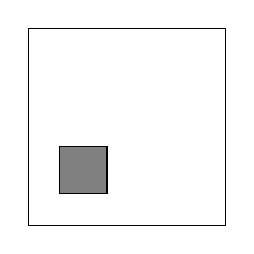
\begin{tikzpicture}	
			\draw [draw=black] (0, 0) rectangle (2.5, 2.5);
			\filldraw [draw=black,fill=gray] (0.4, 0.4) rectangle (1, 1);
		\end{tikzpicture}
		\caption{Informative update ($p$ strictly contained in the CS)}\label{fig1:contained-update}
	\end{subfigure}\hfill
	\begin{subfigure}[b]{.23\linewidth}
		\centering
		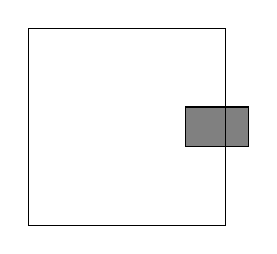
\begin{tikzpicture}	
			\filldraw [draw=black,fill=gray] (2, 1) rectangle (2.8, 1.5);
			\draw [draw=black] (0, 0) rectangle (2.5, 2.5);
		\end{tikzpicture}
		\caption{Informative update ($p$ strictly overlaps with the CS)}\label{fig1:informative-update}
	\end{subfigure}\hfill
	\begin{subfigure}[b]{.23\linewidth}
		\centering
		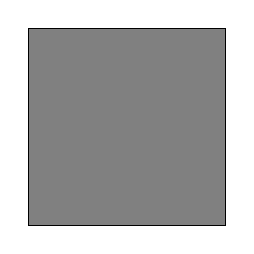
\begin{tikzpicture}	
			\filldraw [draw=black,fill=gray] (0, 0) rectangle (2.5, 2.5);
		\end{tikzpicture}
		\caption{Uninformative update ($p$ equal to the CS)}\label{fig1:uninformative-equal-update}
	\end{subfigure}\hfill
	\begin{subfigure}[b]{.23\linewidth}
		\centering
		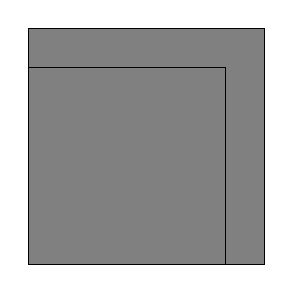
\begin{tikzpicture}	
			\filldraw [draw=black,fill=gray] (0, 0) rectangle (3, 3);
			\filldraw [draw=black,fill=gray] (0, 0) rectangle (2.5, 2.5);
		\end{tikzpicture}
		\caption{Uninformative update ($p$ containing the CS)}\label{fig1:uninformative-update}
	\end{subfigure}
	\caption{A few examples of informative and uninformative updates of the CS. The big squares represent the CS. The grey shapes refer to $p$, the proposition added to the CG (and intersected with the CS to update it).}\label{fig1:informative-assertions}
\end{figure}

\subsection{Dynamic Semantics}

So far, we have mainly considered ``simplex'' assertions that did not make use of operators, connectives or quantifiers. But what about sentences like those in (\ref{ex1:complex-assertions})? How should they interact with the Context Set?
\begin{exe}
	\ex \label{ex1:complex-assertions}
	\begin{xlist}
		\ex {Jo did not grow up in France.}
		\ex {Jo grew up in France or Belgium.}
		\ex {Jo grew up in France and Ed in Belgium.}
	\end{xlist}
\end{exe}

The simplest way to deal with these sentences, would be to compute their intension (the proposition they denote) based on the semantics of negation, disjunction, and conjunction, and then, intersect the resulting proposition with the Context Set. We will call this approach the naive ``bulk'' CS update. There is evidence, coming from the behavior of presuppositions, that this might not be the way to go, and that complex assertions should be added to the Context Set ``bit by bit'' \citep{Heim1982,Heim1983a,Heim1983b}.

To see this, let us consider the pair in (\ref{ex1:presupposition-conj}). The sentences in (\ref{ex1:presupposition-conj}) are conjunctive and only vary in the order of their conjuncts. Additionally, one of their conjuncts contains the presupposition trigger \textit{too}, associated with the predicate \textit{grew up in France}. In the felicitous variant (\ref{ex1:presupposition-conj-good}), \textit{too} occurs in the second conjunct; in the the infelicitous variant (\ref{ex1:presupposition-conj-good}), \textit{too} occurs in the first conjunct. Intuitively, \textit{X too VP} imposes that whatever predicate \textit{VP} denotes be true of at least one individual different from the one \textit{X} denotes. This presupposition can be seen as a precondition on the Context Set (as defined prior to the update step). In the case of (\ref{ex1:presupposition-conj-good}) and (\ref{ex1:presupposition-conj-good}), \textit{Ed too grew up in France} then imposes that the Context Set at the time of the update entail that somebody other than Ed (e.g., Jo) grew up in France. 

\begin{exe}
	\ex \label{ex1:presupposition-conj}
	\begin{xlist}
		\ex[] {Jo grew up in France, and Ed too grew up in France.}\label{ex1:presupposition-conj-good}
		\ex[\#] {Ed too grew up in France, and Jo grew up in France.}\label{ex1:presupposition-conj-bad}
	\end{xlist}
\end{exe}

Let us attempt a naive ``bulk'' CS update with sentences (\ref{ex1:presupposition-conj-good})/(\ref{ex1:presupposition-conj-bad}). The first step is to compute (\ref{ex1:presupposition-conj-good})/(\ref{ex1:presupposition-conj-bad})'s presuppositions and (propositional) assertions. The CS, as defined prior to the utterance of (\ref{ex1:presupposition-conj-good})/(\ref{ex1:presupposition-conj-bad}), then gets updated, provided that it verifies (\ref{ex1:presupposition-conj-good})/(\ref{ex1:presupposition-conj-bad})'s presupposition. Let us start with (\ref{ex1:presupposition-conj-good}) and (\ref{ex1:presupposition-conj-bad})'s presuppositional component. We can assume that the presupposition that somebody other than Ed grew up in France projects from inside the conjunctive operator. Under this assumption, both (\ref{ex1:presupposition-conj-good}) and (\ref{ex1:presupposition-conj-bad}) end up imposing that the CS prior to their utterance entail that somebody other than Ed grew up in France. This will in principle \textit{not} be verified. So, the naive ``bulk'' Context Set update correctly predicts the infelicity of (\ref{ex1:presupposition-conj-bad}), but, also, incorrectly predicts (\ref{ex1:presupposition-conj-good}) to be odd. Assuming the presupposition does not project does not address the issue. Under this assumption, both (\ref{ex1:presupposition-conj-good}) and (\ref{ex1:presupposition-conj-bad}) end up being presuppositionless, and the naive ``bulk'' CS update correctly predicts (\ref{ex1:presupposition-conj-good})'s felicity, but also incorrectly predicts (\ref{ex1:presupposition-conj-bad}) to be just as felicitous. So, regardless of how presupposition should exactly behave in complex sentences, the asymmetry between (\ref{ex1:presupposition-conj-good}) and (\ref{ex1:presupposition-conj-bad}) does not seem to be captured by the naive ``bulk'' CS update. 

The linear asymmetry in (\ref{ex1:presupposition-conj}) in fact suggests an alternative, ``bit by bit'' update strategy for complex sentences like conjunctions. If each conjunct were to update the CS one at a time, following the linear order of the sentence, then, the first conjunct of (\ref{ex1:presupposition-conj-good}) would create an updated CS that would incorporate the information that \textit{Jo grew up in France}, and as such verify the presupposition of (\ref{ex1:presupposition-conj-good})'s second conjunct (that somebody other than Ed grew up in France). This would allow (\ref{ex1:presupposition-conj-good})'s second conjunct to be subsequently intersected to the CS, and would predict the whole conjunction in (\ref{ex1:presupposition-conj-good}) to be felicitous. By contrast, (\ref{ex1:presupposition-conj-bad})'s first conjunct would still be problematic in this framework, because its presupposition would not be satisfied by the original CS. 

In this toy example, a presupposition was used as a diagnostic to better determine the nature of the CS update triggered by a conjunctive sentence. The conclusion is that the update should be dynamic: the two conjuncts should be intersected with the CS one by one, in the order in which they appear. This should apply to presuppositionless sentences as well; and is summarized in (\ref{ex1:conj-cs-update}). 


\begin{exe}
	\ex {\textit{Conjunctive update of the CS.} Let $\mathcal{C}$ be a conversation and $CS(\mathcal{C})$ its Context Set. If a sentence $S$ of the form $X \wedge Y$, with $\llbracket X\rrbracket = p$ and $\llbracket Y\rrbracket = q$ is uttered, then a new Context Set $CS''(\mathcal{C})$ is derived by, first intersecting $CS(\mathcal{C})$ with $p$ to create $CS'(\mathcal{C})$, and second, intersecting $CS'(\mathcal{C})$ with $q$ to create $CS''(\mathcal{C})$:\\
		$CS''(\mathcal{C}) = (CS(\mathcal{C}) \cap p) \cap q = CS'(\mathcal{C})\cap q$\\
	The potential presuppositions of $X$ and $Y$ are tested on the CS at the time of their respective update, i.e. on $CS(\mathcal{C})$ and $CS'(\mathcal{C})$ respectively.}\label{ex1:conj-cs-update}
\end{exe}

\textit{Dynamic Semantics} is a framework that proposes to extend this view to other kinds of complex sentences, e.g. disjunctive and conditional sentences. In Dynamic Semantics, sentences give rise to different kinds of CS updates, depending on how they are constructed. More fundamentally, Dynamic Semantics proposes a shift of perspective when it comes to the meaning of assertions: assertions no longer denote propositions, instead they denote proposals to update the CS in specific ways. In that sense, assertions can be seen as functions from an input CS, to an output CS--sometimes called Context-Change Potentials (\textbf{CCP}). CCPs for disjunctive and conditional sentences are spelled out in (\ref{ex1:disj-cs-update}) and (\ref{ex1:cond-cs-update}) respectively.

\begin{exe}
	\ex {\textit{Disjunctive update of the CS.} Let $\mathcal{C}$ be a conversation and $CS(\mathcal{C})$ its Context Set. If a sentence $S$ of the form $X \vee Y$, with $\llbracket X\rrbracket = p$ and $\llbracket Y\rrbracket = q$ is uttered, then a new Context Set $CS'(\mathcal{C})$ is derived by intersecting $CS(\mathcal{C})$ with $p \cup q$:\\
		$CS'(\mathcal{C}) = CS(\mathcal{C}) \cap (p \cup q)$\\
		The potential presuppositions of $X$ and $Y$ are tested on, respectively, $CS(\mathcal{C})$ and $CS(\mathcal{C}) \cap \neg p$.\footnote{There is a debate on whether or not disjunctions should behave symmetrically w.r.t. the presupposition(s) carried by their disjuncts. An alternative, symmetric way to evaluate $X$ and $Y$'s potential presuppositions, would be to test them against $CS(\mathcal{C}) \cap \neg q$ and $CS(\mathcal{C}) \cap \neg p$ respectively.}}\label{ex1:disj-cs-update}
	\ex {\textit{Conditional update of the CS.} Let $\mathcal{C}$ be a conversation and $CS(\mathcal{C})$ its Context Set. If a sentence $S$ of the form \textit{if $X$ then $Y$}, with $\llbracket X\rrbracket = p$ and $\llbracket Y\rrbracket = q$ is uttered, then a new Context Set $CS''(\mathcal{C})$ is derived by, first intersecting $CS(\mathcal{C})$ with $p$ to create $CS'(\mathcal{C})$, and second, intersecting $CS'(\mathcal{C})$ with $q$ to create $CS''(\mathcal{C})$:\\
		$CS''(\mathcal{C}) = (CS(\mathcal{C}) \cap p) \cap q = CS'(\mathcal{C})\cap q$\\
		The potential presuppositions of $X$ and $Y$ are tested on the CS at the time of their respective update, i.e. on $CS(\mathcal{C})$ and $CS'(\mathcal{C})$ respectively.}\label{ex1:cond-cs-update}
\end{exe}


This incremental view of assertions leads to a revised, incremental definition of informativity, given in (\ref{ex1:informativity-ccp}). 

\begin{exe}
	\ex {\textit{Informativity (CCP view).} A sentence $S$ is informative in a conversation $\mathcal{C}$, iff all the updates of $CS(\mathcal{C})$ it gives rise to are non-vacuous.}\label{ex1:informativity-ccp}
\end{exe}

In sum, assertions can be seen as proposals to update (shrink) the CS. The specific update they give rise to is compositionally derived, and incrementally performed, following the structure of the sentence. We will use a similar approach in Chapter \ref{ex1:accommodating -quds} when defining questions \textit{evoked} by assertions. But this first requires to define what questions mean. This is what we do in the next section, in which we show that questions influence, not the size, but rather, the topology of the CS.








\section{Questions indicate which kind of information is worth providing}\label{sec:questions}

\subsection{Questions as answerhood conditions}
Participants in a conversation utter assertions to shrink the CS, and hopefully, jointly figure out which world they are in. But this allows for very unnatural interactions like (\ref{ex1:weird-assertion-sequence}), taking the forms of sequences of intuitively unrelated sentences--as long as each of them denotes propositions shrinking the CS!

\begin{exe}
	\ex {--Jo grew up in France.\\
		--I like cheese.\\
		--Al is arriving tomorrow.}\label{ex1:weird-assertion-sequence}
\end{exe}

This is where questions enter the game. Intuitively, a question indicates an interest in \textit{which} proposition(s) hold, among a restricted set. The proposition at stake are typically possible answers to the question. Questions therefore denote sets of sets of worlds (equivalent to a type $\langle\langle \texttt{s}, \texttt{t}\rangle, \texttt{t}\rangle$), and constrain which kind of (informative) propositions can be uttered as a follow-up. For instance, a polar question such as \textit{Is it raining?} will typically request information of the form \textit{It is raining}, or \textit{It is not raining}, see (\ref{ex1:simple-polar-q}). 

\begin{exe}
	\ex {--Is it raining?\\
	--Yes, it is raining. / No, it is not raining.}\label{ex1:simple-polar-q}
\end{exe} 

The question \textit{Is it raining?} can thus be represented as a set made of two propositions, namely, the proposition that \textit{it is raining}, and the proposition that \textit{it is not raining}.  

\begin{exe}
	\ex {$\llbracket$ Is it raining? $\rrbracket$ = $\lbrace$ $\llbracket$ It is raining $\rrbracket$, $\llbracket$ It is not raining $\rrbracket$ $\rbrace$\\
		\phantom{$\llbracket$ Is it raining? $\rrbracket$} = $\lbrace\lambda w. \ $ it is raining in $w$, $ \ \lambda w. \ $ it is not raining in $w \rbrace$\\
	\phantom{$\llbracket$ Is it raining? $\rrbracket$} : $\langle\langle \texttt{s}, \texttt{t}\rangle, \texttt{t}\rangle$}
\end{exe}

In the case of the question \textit{is it raining?}, the set of possible answers is fairly simple: it only contains two elements.These two elements  cover the space of all possibilities,\footnote{This is the case assuming there is no vagueness-induced ``grey area'', i.e. any salient situation is either a \textit{raining}-situation, or a \textit{not raining}-situation} and are \textit{exclusive}: if it's the case that it's raining (at a salient place, at a salient time) in $w$, then, it's not the case that it is not raining (at the same place, at the same time), in $w$. We will see in the next section that this configuration amounts to a partition of the CS. A definition of exclusivity under the set interpretation of propositions is given in (\ref{ex1:proposition-exclusivity}).

\begin{exe}
	\ex {\textit{Exclusive propositions.} $p : \langle \texttt{s}, \texttt{t}\rangle$ and $q : \langle \texttt{s}, \texttt{t} \rangle$ are exclusive if $p \cap q = \emptyset$.}\label{ex1:proposition-exclusivity}
\end{exe}


But questions may not always intuitively request information about exclusive propositions. For instance, a \textit{wh}-question like \textit{Which students passed the class?} expects answers that convey a subset of students who passed the class, see (\ref{ex1:simple-wh-q}). But there are many possible, overlapping subsets of students, so, the corresponding propositions will be overlapping as well. For instance, the proposition that \textit{Jo passed the class}, denotes the set of worlds in which Jo passed the class, and this set happens to contain the set of worlds where both Jo and Al passed the class. It also overlaps with the set of worlds in which Al passed the class. 

\begin{exe}
	\ex {Which students passed the class?\\
	--Jo did.\\
	--Al did.\\
	--Jo and Al did.}\label{ex1:simple-wh-q}
\end{exe} 

We will call propositions like \textit{Jo passed the class}, and \textit{Jo and Al passed the class}, alternatives associated to the question \textit{Which students passed the class?} Alternatives may be overlapping; and, as we will see, can be obtained from the original question by substituting its \textit{wh}-component (e.g., \textit{which students}), with relevant, same-type material (e.g., students or groups of students).\footnote{It is worth mentioning that the set $\lbrace\lambda w. $ it is raining in $w$, $ \ \lambda w. $ it is not raining in $w \rbrace$ does not strictly speaking correspond to the set of alternatives raised by \textit{Is it raining?} Section \ref{sec:q-derivation} further specifies how alternatives get compositionally derived, and predicts that \textit{Is it raining?} should only give rise to one alternative: $\lambda w. $ it is raining in $w$. The set $\lbrace\lambda w. $ it is raining in $w$, $ \ \lambda w. $ it is not raining in $w \rbrace$ is derived from this singleton alternative \textit{via} the ``pragmatic'' process presented in (\ref{ex1:partition-induced}), in the next Section.}


\begin{exe}
	\ex {Question : $\llbracket$ Which students passed the class? $\rrbracket$\\
		Alternatives: $\lbrace\llbracket$ Jo passed $\rrbracket$, $\llbracket$ Al passed $\rrbracket$, $\llbracket$ Jo and Al passed $\rrbracket$ ... $\rbrace$}
\end{exe}


Why would this overlap between alternative answers be an issue in modeling the meaning of questions? The fact that entailing or merely overlapping propositions should be considered equally good answers does not capture the idea that more specific propositions constitute more exhaustive answers than less specific ones. For instance, answering that \textit{Jo passed}, in theory leaves the fate of the other students undecided--for instance, it does not settle if \textit{Al passed}, or not. Answering that \textit{Jo and Al passed} by contrast, settles Al's fate, in addition to Jo's. Ideally, an answer to \textit{Which students passed?} should explicitly address whether \textit{each} student of the class passed, or not. That would be an exhaustive answer.

\subsection{Questions as partitions of the Context Set}

We have just discussed that, at the semantic level, questions characterize the conditions under which they are answered, i.e. denote a set of potentially overlapping propositions. But, just like we did with assertions, the effect of this semantics on the Context Set has to be defined. There is in fact a deterministic way to change a set of overlapping propositions $P$ (i.e. a set of subsets of the CS), into a set of exclusive subsets of the CS (called \textit{cells}, for reasons made clear in (\ref{ex1:partition-induced})). To do so, one can group in the same cell the worlds of the Context Set that all ``agree'' on all propositions in $P$. This ``agreement'' property amounts to the same-cell relation in (\ref{ex1:same-cell}). This relation is reflexive, symmetric and transitive, i.e. is an equivalence relation (see proof in (\ref{ex1:cell-equiv-relation})). From this, we can conclude that the set of subsets of the CS induced by $P$, obtained by grouping worlds of the CS according to the same-cell relation, forms a partition of the Context Set (see proof in (\ref{ex1:partition-induced})).\footnote{Cells as we defined them are also called equivalence classes. It's a general property that equivalence classes induced by an equivalence relation on a certain set on which this relation is defined, will create a partition of the set.} So, on top of being exclusive, cells are non-empty and together cover the CS. We assume that the process changing the set of alternative propositions raised by a question, to a partition of the CS, belongs to pragmatics. So, questions \textit{denote} sets of alternative propositions, and this set \textit{pragmatically induces} a partition structure on the CS.

\begin{exe}
	\ex {\textit{Same-cell relation $\equiv_P$.} Let $P$ be a set of propositions, i.e. a set of subsets of the Context Set ($P \in \mathcal{P}(\mathcal{P}(CS))$, with $\mathcal{P}$ the powerset operation). Let $w$ and $w'$ be two worlds of the Context Set. $w \equiv_{P} w'$ iff, $\forall p \in P. \  p(w) = p(w')$.}\label{ex1:same-cell}
		\ex {$\equiv_P$ is an equivalence relation, no matter what $P$ is. Let $\forall P \in \mathcal{P}(\mathcal{P}(CS))$.
		\begin{itemize}
			\item $\equiv_P$ is reflexive: $\forall w \in CS. \ \forall p \in P. \  p(w) = p(w)$.
			\item $\equiv_P$ is symmetric. Let $\forall (w, w') \in CS^2$.\\ $\forall p \in P. \  p(w) = p(w')$ iff $\forall p \in P. \  p(w') = p(w)$.
			\item $\equiv_P$ is transitive. Let $\forall (w, w', w'') \in CS^3$.\\
			We assume $\forall p \in P. \  p(w) = p(w')$ and $\forall p \in P. \  p(w') = p(w'')$.\\Let $\forall p \in P$. 
			We have $p(w) = p(w')$ and $p(w') = p(w'')$, so $p(w') = p(w'')$.\\
			So, $\forall p \in P. \  p(w) = p(w'')$
	\end{itemize}}\label{ex1:cell-equiv-relation}
	\ex {\textit{Partition of the CS induced by $P$.\footnote{ \citet{Fox2018} proposes an alternative way to derive a partition of the CS from a set of alternative propositions, leveraging the covert operator \textit{exh}}} Let $P$ be a set of propositions. The partition induced by $P$ in the Context Set is the set of subsets of the CS (cells): $\mathfrak{P}_{P, CS} =  \lbrace \lbrace w' \ | \ w' \in CS \wedge w' \equiv_P w \rbrace \ | \ w \in CS\rbrace$. This set partitions the CS.
	\begin{itemize}
		\item No cell $c$ of $\mathfrak{P}_{P, CS}$ is empty. Let $c \in \mathfrak{P}_{P, CS}$. There is a $w \in CS$ s.t. $c = \lbrace w' \ | \ w' \in CS \wedge w' \equiv_P w \rbrace$. Then at least $w \in c$, because $w \equiv_P w$.
		\item Cells cover the CS. Let $w \in CS$. $\mathfrak{P}_{P, CS}$ contains a cell $c = \lbrace w' \ | \ w' \in CS \wedge w' \equiv_P w \rbrace$. Then $w \in c$ because $w \equiv_P w$.
		\item Cells are disjoint. Let $(c, c') \in \mathfrak{P}_{P, CS}$, s.t. $c \cap c' \neq \emptyset$. We show $c = c'$. $c$ and $c'$ have resp. the form $c = \lbrace w'' \ | \ w'' \in CS \wedge w'' \equiv_P w \rbrace$ and $c = \lbrace w'' \ | \ w'' \in CS \wedge w'' \equiv_P w' \rbrace$, for $(w, w') \in CS^2$. Let $w''' \in c \cap c'$. Then $w''' \equiv_P w$ and $w''' \equiv_P w'$, and so by symmetry and transitivity, $w \equiv_P w'$, and $c=c'$.
		\end{itemize}}\label{ex1:partition-induced}
\end{exe}

It is easy to show that, in the polar example (\ref{ex1:simple-polar-q}), the subsets of the CS defined by \textit{It is raining} and \textit{It is not raining}, which we said were intuitive answers to the question, form a partition of the CS. Section \ref{sec:q-derivation} will in fact show that polar questions of the form $p?$ \textit{denote} the singleton set formed by $p$, and \textit{induce} a $2$-cell partition of the form $\lbrace p, \neg p\rbrace$.


Let us now see how the above definitions apply to a \textit{wh}-question like \textit{Which students passed?} in (\ref{ex1:simple-wh-q}). Let's assume there are only two salient students, Jo and Al. We assume that the alternatives the question raises (labeled $P$), are the proposition that \textit{Jo passed}, and the proposition that \textit{Al passed}. We assume that the CS contains six possible worlds, which vary according to whether Jo, Al, both, or none passed the class. The worlds may vary in other respects, that are not relevant to us here. The alternatives and cells associated with this question are given in (\ref{ex1:wh-partition-computation}). The alternative set $P$ then corresponds to two subsets of the CS, which do not cover it. In particular, the world in which nobody passed ($w_0$) is included in none of the two alternatives. Moreover, the two subsets are overlapping: both \textit{Jo passed} and \textit{Al passed} contain $w_4$, $w_5$, and $w_6$. Now turning to the cells induced by $P$ on the CS, we notice that there are four of them, which correspond to worlds where nobody, only Jo, only Al, or both Jo and Al passed the class. Such cells cover the CS, are disjoint, and non-empty, so correctly form a partition of the CS. They also fully specify, for \textit{both} Jo and Al, if they passed the class; and as such constitute exhaustive answers to the original question.

\begin{exe}
	\ex {Question : \textit{Which students passed the class?}\\
	Context Set: $\lbrace w_0, w_1, w_2, w_3, w_4, w_5, w_6\rbrace$, s.t.:
	\begin{itemize}
		\item Nobody passed in $w_0$;
		\item Only Jo passed in $w_1$ and $w_2$;
		\item Only Al passed in $w_3$;
		\item Both Jo and Al passed in $w_4$, $w_5$, and $w_6$.
	\end{itemize}
	Alternatives ($P$): $\lbrace$$\llbracket$Jo passed$\rrbracket$, $\llbracket$Al passed$\rrbracket$$\rbrace$ = $\lbrace \lbrace w_1, w_2, w_4, w_5, w_6\rbrace, \lbrace w_3, w_4, w_5, w_6 \rbrace\rbrace$\\
	Cells induced by $\equiv_P$: $\lbrace \lbrace w_0\rbrace, \lbrace w_1, w_2 \rbrace, \lbrace w_3 \rbrace, \lbrace w_4, w_5, w_6\rbrace\rbrace$
	}\label{ex1:wh-partition-computation}
\end{exe}
\begin{figure}[H]
	\centering
		\begin{subfigure}[t]{.27\linewidth}
		\centering
		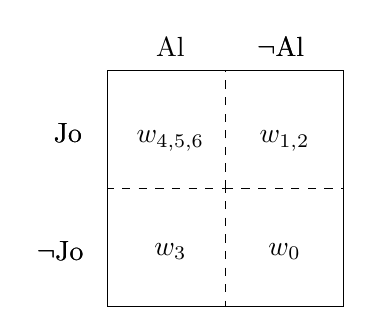
\begin{tikzpicture}	
			\node[] at(.8, 3.3) {Al};
			\node[] at(2.2, 3.3) {$\neg$Al};
			\node[] at(-.6, .7) {$\neg$Jo};
			\node[] at(-.5, 2.2) {Jo};
			
			\node[] at(.8,2.1) {$w_{4, 5, 6}$};
			\node[] at(2.25,2.1) {$w_{1, 2}$};
			\node[] at(.8,.7) {$w_{3}$};
			\node[] at(2.25,.7) {$w_{0}$};
			
			\node[] at(2.2, 3.3) {$\neg$Al};
			\node[] at(-.6, .7) {$\neg$Jo};
			\node[] at(-.5, 2.2) {Jo};
			\draw [draw=black] (0, 0) rectangle (3, 3);
			\draw [draw=black,dashed] (0, 0) rectangle (1.5, 1.5);
			\draw [draw=black, dashed] (1.5, 1.5) rectangle (3, 3);
		\end{tikzpicture}
		\caption{Distribution of $w_0 ... w_6$ in the CS.}\label{fig1:cs-worlds}
	\end{subfigure}\hfill
	\begin{subfigure}[t]{.27\linewidth}
		\centering
		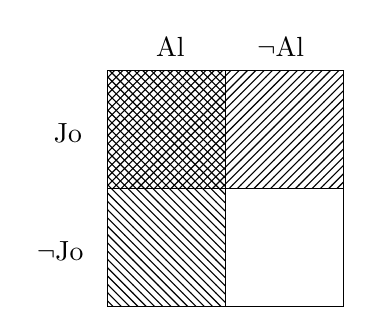
\begin{tikzpicture}	
			\node[] at(.8, 3.3) {Al};
			\node[] at(2.2, 3.3) {$\neg$Al};
			\node[] at(-.6, .7) {$\neg$Jo};
			\node[] at(-.5, 2.2) {Jo};
			\draw [draw=black] (0, 0) rectangle (3, 3);
			\draw [draw=black,pattern=north west lines] (0, 0) rectangle (1.5, 3);
			\draw [draw=black,pattern=north east lines] (0,1.5) rectangle (3, 3);
		\end{tikzpicture}
		\caption{Alternatives: 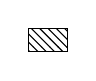
\begin{tikzpicture}
				\draw [draw=black,pattern=north west lines] (0, 0) rectangle (.5, .3);
		\end{tikzpicture} defines \textit{Al passed} and 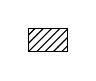
\begin{tikzpicture}
		\draw [draw=black,pattern=north east lines] (0, 0) rectangle (.5, .3);
		\end{tikzpicture} defines \textit{Jo passed} }\label{fig1:alternatives}
	\end{subfigure}\hfill
	\begin{subfigure}[t]{.41\linewidth}
		\centering
		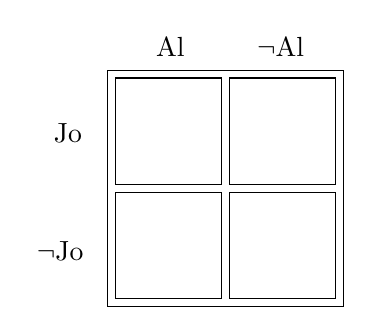
\begin{tikzpicture}	
			\node[] at(.8, 3.3) {Al};
			\node[] at(2.2, 3.3) {$\neg$Al};
			\node[] at(-.6, .7) {$\neg$Jo};
			\node[] at(-.5, 2.2) {Jo};
			\draw [draw=black] (0, 0) rectangle (3, 3);
			\draw [draw=black] (0.1, 1.55) rectangle (1.45, 2.9);
			\draw [draw=black] (1.55, 0.1) rectangle (2.9, 1.45);
			\draw [draw=black] (0.1, 0.1) rectangle (1.45, 1.45);
			\draw [draw=black] (1.55, 1.55) rectangle (2.9, 2.9);
		\end{tikzpicture}
		\caption{Partition induced by 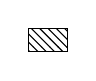
\begin{tikzpicture}
				\draw [draw=black,pattern=north west lines] (0, 0) rectangle (.5, .3);
			\end{tikzpicture} and 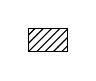
\begin{tikzpicture}
				\draw [draw=black,pattern=north east lines] (0, 0) rectangle (.5, .3);
		\end{tikzpicture}. Cells correspond to the subsets of Figure \ref{fig1:alternatives} featuring the same overall pattern. }\label{fig1:cells}
	\end{subfigure}
\caption{Partitioning of the CS defined in (\ref{ex1:wh-partition-computation}) according to the alternatives \textit{Jo passed} and \textit{Al passed}. The CS is organized as follows: counter-clockwise, quadrant I is made of \textit{Jo but not Al}-worlds; quadrant II, \textit{Jo and Al}, quadrant III, \textit{Al but not Jo}, and quadrant IV, \textit{neither Jo nor Al}.}
\end{figure}


To summarize, at the pragmatic level questions are partitions of the Context Set, as formalized in (\ref{ex1:question-partition}).\footnote{It is important to note that questions may be taken to have a partition \textit{semantics}. But we do not cover this here.} The cells of such partitions constitute maximal answers to the questions. Unions of two or more cells constitute non-maximal answers, as defined in (\ref{ex1:question-answer}).

\begin{exe}
	\ex {\textit{Standard semantics for questions \citep{Jager1996,Hulstijn1997,Groenendijk1984,Groenendijk1999}.}	Given a conversation $\mathcal{C}$ and a Context Set $CS(\mathcal{C})$, a question on $CS(\mathcal{C})$ is a partition of $CS(\mathcal{C})$, i.e. a set of subsets of $CS(\mathcal{C})$ (``cells'') $\lbrace c_1, ..., c_k\rbrace$ s.t.:
		\begin{itemize}
			\item ``No empty cell'': $\forall i \in [1; k]. \ c_i \neq \emptyset$
			\item ``Full cover'': $\bigcup_{i\in[1;k]} c_i = CS(\mathcal{C})$
			\item ``Pairwise disjointness'': $\forall (i, j) \in [1;k]^2. \ i \neq j \Rightarrow c_i \cap c_j = \emptyset$
		\end{itemize}
	}\label{ex1:question-partition}
	\ex {\textit{Maximal and non-maximal answers to a question.} Given a conversation $\mathcal{C}$, a Context Set $CS(\mathcal{C})$, and a question $Q$ forming a partition $\lbrace c_1, ..., c_k\rbrace$ of $CS(\mathcal{C})$:
		\begin{itemize}
			\item Any $c \in \lbrace c_1, ..., c_k\rbrace$ constitutes a maximal answer to $Q$;
			\item Any $c'$ s.t. $\exists C \subseteq \lbrace c_1, ..., c_k\rbrace. \ |C| > 1 \wedge c' = \bigcup C$ is a non-maximal answer to $Q$.
		\end{itemize}
	}\label{ex1:question-answer}
\end{exe}

Just like we did with assertions, let us clarify further what it means to be a good question. We have established that the idea of a partition is a good candidate to model the effect of questions on a given CS. But what if the CS is already such that the partition induced by the question's alternatives is just made of one big cell? Such a configuration suggests that the question is already \textit{settled}, meaning, the CS already makes one maximal answer trivial. For instance, if it is already common ground between the conversation's participants that \textit{it is raining} (at the salient place and time) in (\ref{ex1:simple-polar-q}), then, the question \textit{Is it raining?} appears completely trivial. This is illustrated in Figure \ref{fig1:trivial-q} and generalized in (\ref{ex1:trivial-question}).


\begin{figure}[H]
	\centering
	\begin{subfigure}[t]{.27\linewidth}
		\centering
		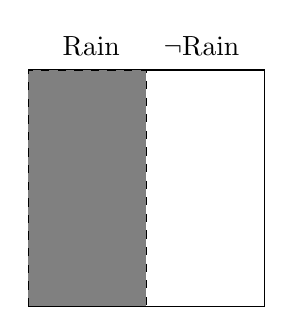
\begin{tikzpicture}	
			\node[] at(.8, 3.3) {Rain};
			\node[] at(2.2, 3.3) {$\neg$Rain};
			\draw [draw=black] (0, 0) rectangle (3, 3);
			\filldraw [draw=black,dashed,fill=gray] (0, 0) rectangle (1.5, 3);
		\end{tikzpicture}
		\caption{Interecting the proposition that \textit{It's raining} (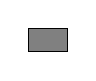
\begin{tikzpicture}
				\filldraw [draw=black,fill=gray] (0, 0) rectangle (.5, .3);
			\end{tikzpicture}) with a CS that is agnostic about the weather.}\label{fig1:cs-raining-not-raining}
	\end{subfigure}\hfill
	\begin{subfigure}[t]{.27\linewidth}
		\centering
		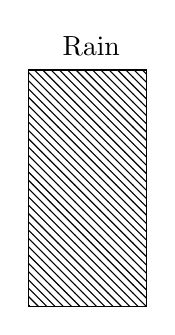
\begin{tikzpicture}	
			\node[] at(.8, 3.3) {Rain};
			\draw [draw=black,pattern=north west lines] (0, 0) rectangle (1.5, 3);
		\end{tikzpicture}
		\caption{Alternatives on the restricted CS: 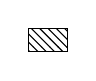
\begin{tikzpicture}
				\draw [draw=black,pattern=north west lines] (0, 0) rectangle (.5, .3);
			\end{tikzpicture} defines \textit{It's raining}.}\label{fig1:alternatives-raining}
	\end{subfigure}\hfill
	\begin{subfigure}[t]{.36\linewidth}
		\centering
		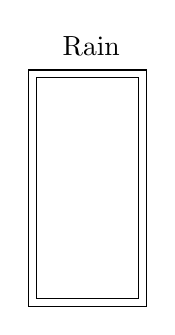
\begin{tikzpicture}	
			\node[] at(.8, 3.3) {Rain};
			\draw [draw=black] (0, 0) rectangle (1.5, 3);
			\draw [draw=black] (0.1, 0.1) rectangle (1.4, 2.9);
		\end{tikzpicture}
		\caption{Partition induced by 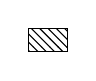
\begin{tikzpicture}
				\draw [draw=black,pattern=north west lines] (0, 0) rectangle (.5, .3);
			\end{tikzpicture} on the CS. Cells correspond to the subsets of Figure \ref{fig1:alternatives-raining} featuring the same overall pattern ($1$ such subset). }\label{fig1:cells-raining}
	\end{subfigure}
	\caption{Updating the CS with the proposition that \textit{It's raining}, and then computing the partition induced by \textit{Is it raining} on the resulting ``shrunk'' CS. The outcome is a single-cell partition, i.e., the question has a trivial pragmatics.}\label{fig1:trivial-q}
\end{figure}


\begin{exe}
	\ex {\textit{Trivial question.} Let $\mathcal{C}$ be a conversation, $CS(\mathcal{C})$ its associated Context Set, and $Q$ a question. $Q$ is trivial given $CS(\mathcal{C})$ iff the partition induced by $Q$ on $CS(\mathcal{C})$ is made of a singleton cell, i.e. has cardinal $1$.}\label{ex1:trivial-question}
\end{exe}

We now have a basic notion of what it mean to be a good assertion, given a CS, and a good question, given a CS. A good assertion has to be informative, i.e. properly shrink the CS (as per (\ref{ex1:informativity})/(\ref{ex1:informativity-ccp})). A good question has to induce a non-trivial, multiple-cell partition on the CS (as per (\ref{ex1:trivial-question})). But being a good question or a good assertion, does not \textit{only} depend on the state of the CS! In particular, good assertions also have to be good answers to good questions. This principle, dubbed \textit{Question-Answer Congruence}, is given in (\ref{ex1:q-a-congruence}).

\begin{exe}
	\ex {\textit{Question-Answer Congruence \citep{Katzir2015}.} A felicitous assertion has to be a good answer to a good question.}\label{ex1:q-a-congruence}
\end{exe}

The next Section presents what can be seen as a partial implementation of this principle, in the form of a general principle dubbed \textsc{Relevance}. It also points out the limitations of this principle.


\section{Assertions as good answers to questions}\label{sec:q-a-interaction}


\subsection{Relevance mediate questions and assertions}
Now that we precisified what assertions and questions are, it becomes possible to (at least partially) define what a good assertion should be, given a question. The principles we introduce in this Section are based on the general concept of \textsc{Relevance}. They will eventually rule out informative but ``unnatural'' sequences of assertions like (\ref{ex1:weird-assertion-sequence}), but also, more generally, a wide range of odd question-answer pairs.

Following much previous literature \citep{VanKuppevelt1995a,VanKuppevelt1995b,Roberts1996,Roberts2012,Ginzburg1996,Buring2003}, we call the question against which assertions are evaluated, \textit{Question under Discussion} (henceforth \textbf{QuD}). QuDs are typically seen as partitions of the CS. In
(\ref{ex1:question-answer}), we defined cells an unions of cells as respectively maximal and non-maximal answers to a question. Very broadly, \textsc{Relevance} constrains what a proposition should do to the cells of the QuD. Let us now unpack this with an example.

If for instance the QuD is about which country Jo grew up in (as in (\ref{ex1:qud-country})), the CS will be partitioned according to propositions of the form \textit{Jo grew up in c}, with \textit{c} a country. Utterances such as (\ref{ex1:france-relevant}) or (\ref{ex1:france-belgium-relevant}), both seem relevant to that kind of QuD, and both constitute answers to the QuD--maximal, or not. By contrast, utterances such as (\ref{ex1:native-irrelevant}), (\ref{ex1:wine-irrelevant}) or (\ref{ex1:cat-irrelevant}), do not appear relevant, and do \textit{not} constitute answers to the QuD: there are native and non-native French speakers in virtually all countries; same holds for wine-lovers and wine-haters; as for (\ref{ex1:cat-irrelevant}) it seems completely independent from the subject matter.\footnote{It is interesting to note that (\ref{ex1:native-irrelevant}) and (\ref{ex1:wine-irrelevant}) can be more easily coerced into relevance than (\ref{ex1:cat-irrelevant}). For instance with (\ref{ex1:native-irrelevant}), one might consider that France is the country which, in proportion, comprises the most native French speakers, and so (\ref{ex1:native-irrelevant}) may be understood as \textit{It is likely that Jo grew up in France}--which constitutes a modalized answer to the QuD. This kind of reasoning is harder (if not impossible) to perform when facing an utterance like (\ref{ex1:cat-irrelevant}).} These various configurations are sketched in Figure \ref{fig1:relevance-example}.

\begin{exe}
	\ex {QuD: In which country did Jo grow up?}\label{ex1:qud-country}
	\begin{xlist}
		\ex[] {Jo grew up in France.}\label{ex1:france-relevant}
		\ex[] {Jo grew up in France or Belgium.}\label{ex1:france-belgium-relevant}
		\ex[??] {Jo speaks French natively.}\label{ex1:native-irrelevant}
		\ex[??] {Jo enjoys wine.}\label{ex1:wine-irrelevant}
		\ex[\#] {The cat went outside.}\label{ex1:cat-irrelevant}
	\end{xlist}
\end{exe}

\begin{figure}[H]
	\centering
	\begin{subfigure}[r]{.24\linewidth}
		\centering
		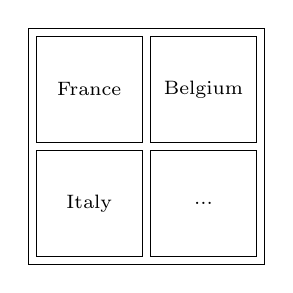
\begin{tikzpicture}	
			\draw [draw=black] (0, 0) rectangle (3, 3) ;
			\draw [draw=black] (0.1, 1.55) rectangle (1.45, 2.9) node[pos=.5] {\scriptsize France};
			\draw [draw=black] (1.55, 0.1) rectangle (2.9, 1.45) node[pos=.5] {\scriptsize ...};
			\draw [draw=black] (0.1, 0.1) rectangle (1.45, 1.45) node[pos=.5] {\scriptsize Italy};
			\draw [draw=black] (1.55, 1.55) rectangle (2.9, 2.9) node[pos=.5] {\scriptsize Belgium};
		\end{tikzpicture}
		\caption{QuD for \textit{In which city did Jo grow up?}}
	\end{subfigure}\hfill
		\begin{subfigure}[r]{.24\linewidth}
			\centering
		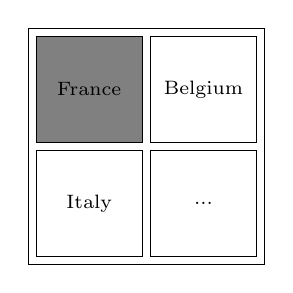
\begin{tikzpicture}	
			\draw [draw=black] (0, 0) rectangle (3, 3) ;
			\filldraw [draw=black,fill=gray] (0.1, 1.55) rectangle (1.45, 2.9) node[pos=.5] {\scriptsize France};
			\draw [draw=black] (1.55, 0.1) rectangle (2.9, 1.45) node[pos=.5] {\scriptsize ...};
			\draw [draw=black] (0.1, 0.1) rectangle (1.45, 1.45) node[pos=.5] {\scriptsize Italy};
			\draw [draw=black] (1.55, 1.55) rectangle (2.9, 2.9) node[pos=.5] {\scriptsize Belgium};
		\end{tikzpicture}
		\caption{Utterance: \textit{Jo grew up in France.}}
	\end{subfigure}\hfill
	\begin{subfigure}[r]{.24\linewidth}
		\centering
		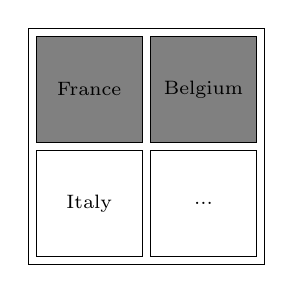
\begin{tikzpicture}	
			\draw [draw=black] (0, 0) rectangle (3, 3) ;
			\filldraw [draw=black,fill=gray] (0.1, 1.55) rectangle (1.45, 2.9) node[pos=.5] {\scriptsize France};
			\draw [draw=black] (1.55, 0.1) rectangle (2.9, 1.45) node[pos=.5] {\scriptsize ...};
			\draw [draw=black] (0.1, 0.1) rectangle (1.45, 1.45) node[pos=.5] {\scriptsize Italy};
			\filldraw [draw=black,fill=gray] (1.55, 1.55) rectangle (2.9, 2.9) node[pos=.5] {\scriptsize Belgium};
		\end{tikzpicture}
		\caption{Utterance: \textit{Jo grew up in France or Belgium.}}
	\end{subfigure}\hfill
	\begin{subfigure}[r]{.24\linewidth}
		\centering
		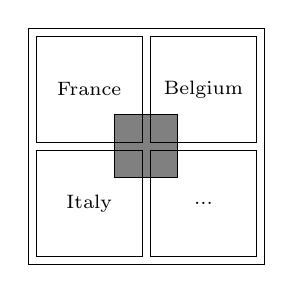
\begin{tikzpicture}	
			\draw [draw=black] (0, 0) rectangle (3, 3) ;
			\filldraw [draw=black,fill=gray] (1.1, 1.1) rectangle (1.9, 1.9) node[pos=.5] {};
			\draw [draw=black] (0.1, 1.55) rectangle (1.45, 2.9) node[pos=.5] {\scriptsize France};
			\draw [draw=black] (1.55, 0.1) rectangle (2.9, 1.45) node[pos=.5] {\scriptsize ...};
			\draw [draw=black] (0.1, 0.1) rectangle (1.45, 1.45) node[pos=.5] {\scriptsize Italy};
			\draw [draw=black] (1.55, 1.55) rectangle (2.9, 2.9) node[pos=.5] {\scriptsize Belgium};
		\end{tikzpicture}
		\caption{Utterance: (\ref{ex1:native-irrelevant}), (\ref{ex1:wine-irrelevant}) or (\ref{ex1:cat-irrelevant}).}
	\end{subfigure}
	\caption{QuD-utterance configurations for a QuD like \textit{In which country did Jo grow up}, and possible follow-up utterance.}\label{fig1:relevance-example}
\end{figure}

From this, we can conclude that a proposition is ``relevant'' to a question, if it constitutes a maximal or a non-maximal answer to the question. This is similar in spirit to the notion of \textit{Aboutness} developed \cite{Lewis1988}, according to which a proposition $p$ is about a subject matter (in modern terms, a QuD), if and only if the truth value of that proposition supervenes on
that subject matter (i.e. $p$ should not introduce truth-conditional distinctions between cellmates, i.e. $p$ does not ``cut across'' cells). This is rephrased in (\ref{ex1:lewis-relevance}). A typical Lewis-relevant configuration is exemplified in Figure \ref{fig1:2-cells-relevant}. It is also worth mentioning that (\ref{ex1:lewis-relevance}) deems propositions contradicting the CS irrelevant (see Figure \ref{fig1:no-cell-relevant}), but in principle does not rule out propositions covering the whole CS (see Figure \ref{fig1:all-cells-relevant}), i.e. uninformative propositions as per (\ref{ex1:informativity}).

\begin{exe}
	\ex {\textsc{Lewis's Relevance (rephrased in the QuD framework).} Let $\mathcal{C}$ be a conversation, $Q$ a QuD defined as a partition of $CS(\mathcal{C})$. Let $p$ be a proposition. $p$ is Lewis-relevant to $Q$, iff $\exists C \subseteq Q. \ p \cap CS(\mathcal{C}) = C$}\label{ex1:lewis-relevance}
\end{exe}


But, coming back to the QuD \textit{In which country did Jo grow up?}, what about an utterance of the form \textit{Jo grew up in Paris?} Although overinformative (the QuD was only asking about countries, not cities!), this utterance appears relevant, because it allows to infer that Jo grew up in France, and not, say, Belgium. This kind of configuration is sketched in Figure \ref{fig1:relevance-example-2}.

\begin{figure}[H]
	\centering
	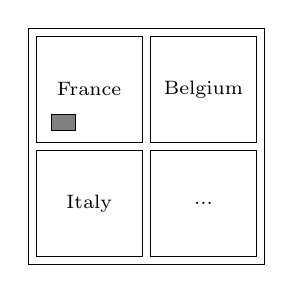
\begin{tikzpicture}	
		\draw [draw=black] (0, 0) rectangle (3, 3) ;
		\draw [draw=black] (0.1, 1.55) rectangle (1.45, 2.9) node[pos=.5] {\scriptsize France};
		\filldraw [draw=black,fill=gray] (0.3, 1.7) rectangle (0.6, 1.9) node[pos=.5] {};
		\draw [draw=black] (1.55, 0.1) rectangle (2.9, 1.45) node[pos=.5] {\scriptsize ...};
		\draw [draw=black] (0.1, 0.1) rectangle (1.45, 1.45) node[pos=.5] {\scriptsize Italy};
		\draw [draw=black] (1.55, 1.55) rectangle (2.9, 2.9) node[pos=.5] {\scriptsize Belgium};
	\end{tikzpicture}
	\caption{QuD-utterance configuration for a QuD like \textit{In which country did Jo grow up?} and an utterance like \textit{Jo grew up in Paris}.}\label{fig1:relevance-example-2}
\end{figure}

The view of relevance, developed by \citet{Roberts2012}, captures this intuition, by stating that a relevant proposition has to rule out at least one maximal answer conveyed by the QuD. In other words, a relevant proposition has to be incompatible with at least one cell of the QuD. This is summarized in (\ref{ex1:roberts-relevance}). This definition makes uninformative propositions irrelevant (see Figure \ref{fig1:all-cells-relevant}), but allows certain propositions that do not coincide with the grand union of a subset of the QuD's cells, to be relevant (see Figures \ref{fig1:sub-cell-relevant} and \ref{fig1:sub-1-cell-relevant}). In other words, relevant propositions in the sense of \citeauthor{Roberts2012} may introduce truth-conditional distinctions between cellmates--as long as they rule out a cell. A particular case is that of propositions like \textit{Jo grew up in Paris}, when the QuD is about countries, which strictly entail a specific cell of the QuD, i.e. are strictly contained in one single cell (see Figure \ref{fig1:sub-cell-relevant}).

\begin{exe}
	\ex {\textsc{Roberts's Relevance \citep{Roberts2012}.} Let $\mathcal{C}$ be a conversation, $Q$ a (non-trivial) QuD defined as a partition of $CS(\mathcal{C})$. Let $p$ be a proposition. $p$ is Roberts-relevant to $Q$, if $\exists c \in Q. \ p \cap c = \emptyset$.
	%\begin{itemize}
		%\item 
		%\item Let $Q'$ be a follow-up question. $Q'$ is Roberts-relevant to $Q$, if each alternative of $Q'$ is Roberts-relevant to $Q$.
	%\end{itemize}
	}\label{ex1:roberts-relevance}
\end{exe}

\begin{figure}[H]
	\centering
	\begin{subfigure}[b]{.3\linewidth}
		\centering
		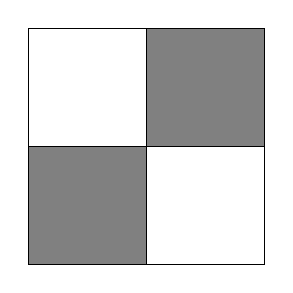
\begin{tikzpicture}	
			\draw [draw=black] (0, 0) rectangle (3, 3);
			\filldraw [draw=black,fill=gray] (0, 0) rectangle (1.5, 1.5);
			\filldraw [draw=black,fill=gray] (1.5, 1.5) rectangle (3, 3);
		\end{tikzpicture}
		\caption{Informative, Lewis-relevant, Roberts-relevant}\label{fig1:2-cells-relevant}
	\end{subfigure}\hfill
	\begin{subfigure}[b]{.3\linewidth}
		\centering
		\begin{tikzpicture}	
			\draw [draw=black] (0, 0) rectangle (3, 3);
			\draw [draw=black] (0, 0) rectangle (1.5, 1.5);
			\draw [draw=black] (1.5, 1.5) rectangle (3, 3);
		\end{tikzpicture}
		\caption{Informative, not Lewis-relevant, Roberts-relevant}\label{fig1:no-cell-relevant}
	\end{subfigure}\hfill
	\begin{subfigure}[b]{.33\linewidth}
		\centering
		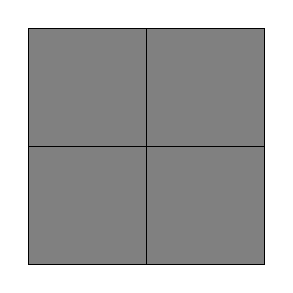
\begin{tikzpicture}	
			\filldraw [draw=black,fill=gray] (0, 0) rectangle (3, 3);
			\draw [draw=black] (0, 0) rectangle (1.5, 1.5);
			\draw [draw=black] (1.5, 1.5) rectangle (3, 3);
		\end{tikzpicture}
		\caption{Uninformative, Lewis-relevant, not Roberts-relevant.}\label{fig1:all-cells-relevant}
	\end{subfigure}
\end{figure}
\begin{figure}[H]\ContinuedFloat
	\begin{subfigure}[b]{.3\linewidth}
		\centering
		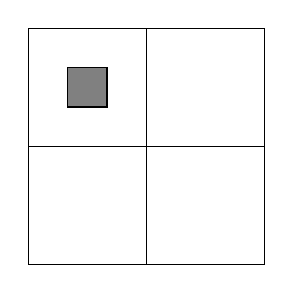
\begin{tikzpicture}	
			\draw [draw=black] (0, 0) rectangle (3, 3);
			\draw [draw=black] (0, 0) rectangle (1.5, 1.5);
			\draw [draw=black] (1.5, 1.5) rectangle (3, 3);
			\filldraw [draw=black,fill=gray] (0.5, 2) rectangle (1,2.5);
		\end{tikzpicture}
		\caption{Informative, not Lewis-relevant, Roberts-relevant}\label{fig1:sub-cell-relevant}
	\end{subfigure}\hfill
	\begin{subfigure}[b]{.3\linewidth}
		\centering
		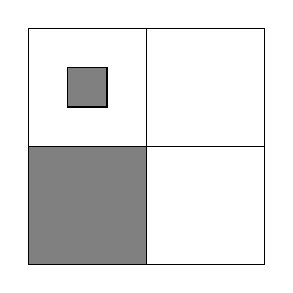
\begin{tikzpicture}	
			\draw [draw=black] (0, 0) rectangle (3, 3);
			\filldraw [draw=black,fill=gray] (0, 0) rectangle (1.5, 1.5);
			\draw [draw=black] (1.5, 1.5) rectangle (3, 3);
			\filldraw [draw=black,fill=gray] (0.5, 2) rectangle (1,2.5);
		\end{tikzpicture}
		\caption{Informative, not Lewis-relevant, Roberts-relevant}\label{fig1:sub-1-cell-relevant}
	\end{subfigure}\hfill
	\begin{subfigure}[b]{.33\linewidth}
		\centering
		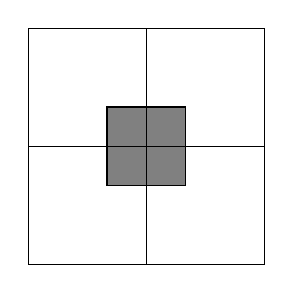
\begin{tikzpicture}	
			\filldraw [draw=black,fill=gray] (1, 1) rectangle (2,2);
			\draw [draw=black] (0, 0) rectangle (3, 3);
			\draw [draw=black] (0, 0) rectangle (1.5, 1.5);
			\draw [draw=black] (1.5, 1.5) rectangle (3, 3);
		\end{tikzpicture}
		\caption{Informative, not Lewis-relevant, not Roberts-relevant}\label{fig1:not-relevant}
	\end{subfigure}
\end{figure}

In sum, the concept of \textsc{Relevance} (whether it follows Lewis's or Roberts's implementation) allows to rule-out a wide range of QuD-utterance pairs, by stating that propositions should properly relate to an existing question. We will not discuss which approach between Lewis's and Roberts's is best here, and will propose an incremental variant of this core concept in Chapter \ref{chap:relevance}, to deal with certain complex, out-of-the blue sentences. The next two section outline a few limitations of relevance.

\subsection{A few conceptual shortcomings of \textsc{Relevance}}

Regardless on which view of \textsc{Relevance} is adopted, relevant propositions can be added to the Common Ground, and as such, trigger an update of the CS. This, in turn, updates the QuD, which must remain a partition of the CS. It is easy to show, given how partition are ``induced'' on a set (see definition (\ref{ex1:partition-induced})), that the updated QuD on the smaller CS corresponds to the previous QuD, whose cells are pointwise intersected with the newly added proposition, and such that empty cells are filtered. This is formalized in (\ref{ex1:partitioned-context-set-update}).

\begin{exe}
	\ex{\textit{Updating the partitioned Context Set.} Let $\mathcal{C}$ be a conversation, $CS(\mathcal{C})$ its Context Set, and let $Q$ be a partition of $CS(\mathcal{C})$. If a sentence $S$ denoting $p$ is uttered and relevant given $Q$ (as per (\ref{ex1:lewis-relevance}) or (\ref{ex1:roberts-relevance})), then a new Context Set $CS'(\mathcal{C})$ is derived by intersecting $CS(\mathcal{C})$ with $p$, and this new context set is partitioned by $Q'$, s.t.:\\
		$Q' = \lbrace c' \ | \ \exists c \in Q. \ c' = c \cap p \wedge c' \neq \emptyset\rbrace$}\label{ex1:partitioned-context-set-update}
\end{exe}

There are two shortcomings to the current framework. First, adding a proposition to  the CG ``mechanically'' leads to an update of the CS and of the QuD, but does not directly affect the \textit{structure} of this QuD: even if some cells should shrink, the \textit{limits} of each cell remain the same. This goes against the intuition that sometimes, sentences give rise rise to brand new QuDs, as exemplified by the exchange in (\ref{ex1:followup-qud}).

\begin{exe}
	\ex {--Is it raining?\\
	--Yes, I think so. I just so Ed come in with this very pretty umbrella.\\
	(Likely follow-up: Where did Ed find this umbrella?)}\label{ex1:followup-qud}
\end{exe}


Second, and relatedly, one can wonder what is supposed to happen in the case of out-of-the-blue sentences, i.e. sentences for which there is no explicit QuD. In such cases, it is generally assumed that a reasonable QuD is somehow inferred. But, given the fact that a QuD is merely a partition of the current CS, there exists many options. This dissertation will focus on how exactly QuDs are inferred, what additional constraints hold between an assertion and a QuD, and what the consequences are for pragmatic theory.

\subsection{Relevance and the packaging of information}
We start by showing that the felicity of disjunctions and conditionals is sensitive to \textit{overt} QuDs -- but in different ways. We take this as evidence that out-of-the-blue disjunctions and conditionals accommodate different kinds of implicit QuDs.\\

If a context contrasting \textit{Paris} and \textit{France but not Paris} is set as in (\ref{ex1:qud-setting}), (\ref{ex1:hc-ns-w}) and (\ref{ex1:ldhc-ns-w}) improve (see \cite{Haslinger2023} for similar effects on disjunctions and conjunctions). This is strange: even if the context and question made \textit{Paris} (but no other French city) a relevant alternative to \textit{France}, \textit{exh} would remain IW in the consequent of (\ref{ex1:hc-ns-w}): \textit{if Jo did not grow up in Paris, she grew up in France but not Paris}, is equivalent to \textit{if Jo did not grow up in Paris, she grew up in France}. In other words, \textit{exh} (as constrained by IW) cannot leverage the contextually provided alternatives to make (\ref{ex1:hc-ns-w}) escape SR in (\ref{ex1:qud-setting}). The same applies to (\ref{ex1:ldhc-ns-w}).


\begin{exe}
	\ex{\textit{Context: French accents vary across countries and between Paris the rest of France.}\\
		Al: I'm wondering where Jo learned French.\\
		Lu: I'm not completely sure but... (\ref{ex1:hc-ns-w}) \cmark (\ref{ex1:ldhc-ns-w}) \cmark}\label{ex1:qud-setting}
\end{exe}


This suggests that a purely LF-based view of redundancy such as SR, may be insufficient to capture the interaction between HCs and how their context of utterance packages information. Rather, it seems that the context of (\ref{ex1:qud-setting}) makes a specific partition of the CS salient, and that this partition can be used to make otherwise infelicitous assertions accommodate a different question than the one they would evoke out-of-the-blue.

Additionally, conditionals and disjunctions seem to accommodate distinct QuDs. To show this, we use the construction \textit{depending on Q, p} (\cite{Karttunen1977,Kaufmann2016}), where \textit{Q} is a question and \textit{p} a proposition. This construction has been argued to force the partition conveyed by Q to match specific live issues raised by $p$. We understand such ``live issues'' as the maximal true answers of the QuD evoked by $p$. The contrast between (\ref{ex1:depending-on-or}) and (\ref{ex1:depending-on-if}) then suggests that the \textit{France} and \textit{Belgium} answers can be matched against \textit{Q} in the disjunctive, but not in the conditional case. This in turn means that a disjunction introduces a QuD making both disjuncts maximal true answers, while a conditional does not do the same with its consequent and the negation of its antecedent.

\begin{exe}
	\ex\label{ex1:depending-on} Depending on $[$how her accent sounds like$]_{Q}$...
	\begin{xlist}
		\ex {Jo grew up in France \textbf{or} in Belgium. \hfill \p{}$\vee$\q }\label{ex1:depending-on-or}
		\ex[??]{\textbf{if} Jo didn't grow up in France she grew up in Belgium. \hfill $\neg$\p{}$\rightarrow$\q} \label{ex1:depending-on-if}
		\ex[?] {\textbf{if} Jo didn't grow up in France, she grew up in Belgium \textbf{or} in Québec. \hfill $\neg$\p{}$\rightarrow$(\q$\vee$\r)}\label{ex1:depending-on-if-or}
		\ex [??]{\textbf{if} Jo didn't grow up in France \textbf{or} Belgium, she grew up in Québec. \hfill $\neg$(\p$\vee$\q)$\rightarrow$\r}\label{ex1:depending-on-or-if}
	\end{xlist}
\end{exe}


The existence of an improvement between (\ref{ex1:depending-on-if}) and (\ref{ex1:depending-on-if-or}), and the absence of a similar improvement in between (\ref{ex1:depending-on-if}) and (\ref{ex1:depending-on-or-if}), also implies that the answers targeted by \textit{depending on Q}, when \textit{p} is conditional, are the ones made available by the consequent of \textit{p} (which is appropriately disjunctive in (\ref{ex1:depending-on-if-or}), but not (\ref{ex1:depending-on-or-if})).


More generally, this predicts ``connectivity effects'' in disjunctions-of-conditionals, in that the antecedents and consequents respectively have to address similar QuDs; and no such effect in conditionals-of-disjunctions, in that disjuncts coming from the antecedent and consequent may be inquisitively unrelated.


\section{Roadmap of the dissertation}

Specifically, we will claim that instead of being a ``good'' answer to \textit{some} QuD, an out-of-the-blue sentence must be a good answer to a \textit{good} QuD, following insight by \citet{Katzir2015}. We will show that operationalizing this principle allows to account for a wider range of oddness phenomena, that previous approaches struggled to capture under the same umbrella.

 ``Good'' QuDs are determined from the shape of the assertive sentence itself. This is pushing the idea that assertions evoke alternatives one step further, in the sense that sentences will be taken to evoke questions (themselves derived from alternatives). These evoked questions will have a structure that consists in a generalization of the partition structure, namely, they will take the form of parse tree of the CS. We will additionally claim the process deriving good questions from good answers, is subject to constraints that go beyond relevance, and cover concepts such as redundancy. These constraints will make way for a ``lifted'' view of pragmatic oddness, under which an assertion is not odd \textit{per se}, but rather, is odd due to its interaction with the QuDs it evokes. Before presenting the core components of our model, we will briefly present two recent accounts of oddness based on similar ideas.



%
%
%idea that questions and quds are diff
%questions may not denote partitions (evidence from embedding, with surprise, surprise whi not p diff from surprise who p)
%qud are partitions
%
%null hypothesis: the qud is contextually provided, it's always "out there", or, there is an overt question and the sentence gets matched against it.
%
%we explore an alternative (from katzir and singh): we have this idea qs and sentences are linked, but we dont force everything to be in the semantics
% rather, sentences have to obey constraints, that are also influences by the qs the sentnece gives rise to
% 



\section{Appendix: computing questions from propositions}\label{sec:q-derivation}

So far, we have described what could be a reasonable model for questions, in the form of partitions of the CS. But this was done without explaining how exactly such partitions are derived from the Logical Form of questions. This sketches how this is done, while further clarifying the distinction between propositions, alternatives, and questions. We will show that questions are standardly derived from closely related propositions, by abstracting over specific variables.

We will use the question \textit{In which country did Jo grow up?} as an example. The LF associated with this question is given in Figure \ref{fig1:question-lf}.

\begin{figure}[H]
	\centering
	\begin{forest}
		[\fbox{5}[$\lambda_1$][\fbox{4}[{(In which country)$_2$}] [\fbox{3}[$\lambda_2$] [\fbox{2}[[?][$t_1$]] [{\fbox{1}}[Jo][[grew up][$t_2$]]]]]]]
	\end{forest}
	\caption{LF of the question \textit{In which country did Jo grow up?}}\label{fig1:question-lf}
\end{figure}

This question involves a \textit{wh}-phrase (\textit{in which country}), which syntactically originates in an adjunct of \textit{grow up}. It is assumed that the \textit{wh}-phrase leaves a trace $t_2$ in this position. The semantics assigned to the \textit{wh}-phrase is existential, and akin to \textit{some country}. Specifically, \textit{in which country} takes a predicate of type $\langle \texttt{e}, \texttt{t} \rangle$ as argument, and returns the quantified statement that \textit{some country} verifies the predicate.

\begin{exe}
	\ex {$\llbracket$In which country$\rrbracket^w$ = $\lambda P. \ \exists l. \ l \text{ is a country in } w \wedge P(l) = 1$}
\end{exe}

The \textit{wh}-phrase outscopes another ``proto-question'' operator \citep{Karttunen1977}. This operator takes two propositions (here, the trace $t_1$ and the proposition that \textit{Jo grew up in $t_2$}), and simply equates them. 

\begin{exe}
	\ex {$\llbracket$?$\rrbracket^w$ = $\lambda p. \ \lambda q. \ p = q$}
\end{exe}

Applying this operator successively to $t_1$ and the intension of \fbox{1}, yields the following.

\begin{exe}
	\ex {\fbox{1} = $\llbracket$Jo grew up $t_2$$\rrbracket^w = 1 \text{ iff Jo grew up in $t_2$ in $w$}$}
	\ex {\fbox{2} = $\llbracket$? $t_1$ Jo grew up $t_2$$\rrbracket^w = 1 \text{ iff } t_1 = \lambda w'. \text{ Jo grew up in $t_2$ in $w'$}$}
\end{exe}

Abstraction then applies to \fbox{2}, binds $t_2$ and yields a predicate that can then serve as an argument of the \textit{wh}-phrase. The \textit{wh}-phrase then turns this predicate into an existentially quantified expression targeting the element being questioned (here, a country).

\begin{exe}
	\ex {\fbox{3} = $\llbracket$ $\lambda_2$ ? $t_1$ Jo grew up $t_2$$\rrbracket^w = \lambda l. \ t_1 = \lambda w'. \text{ Jo grew up in $l$ in $w'$}$}
	\ex {\fbox{4} = $\llbracket$ In which country ... Jo grew up $t_2$$\rrbracket^w$\\
		\phantom{\fbox{4}}	= $\exists l. \ \text{$l$ is a country in $w$} \wedge t_1 = \lambda w'. \text{ Jo grew up in $l$ in $w'$}$}
\end{exe}

Lastly, a $t_1$ gets bound to produce a set of propositions, namely, the set of propositions that coincide with the proposition that \textit{Jo grew up in l}, for some country $l$. 

\begin{exe}
	\ex {\fbox{5} = $\llbracket$ $\lambda_1$ In which country ... Jo grew up $t_2$$\rrbracket^w$\\
		\phantom{\fbox{5}}	= $\lambda p. \ \exists l. \ \text{$l$ is a country in $w$} \wedge p = \lambda w'. \text{ Jo grew up in $l$ in $w'$}$\\
		\phantom{\fbox{5}} $\simeq$ $\lbrace p \ | \ \exists l. \ \text{$l$ is a country in $w$} \wedge p = \lambda w'. \text{ Jo grew up in $l$ in $w'$}\rbrace$
	}
\end{exe}

This example showed that the semantics of a question is derived from that of its ``assertive counterpart'', where the \textit{wh}-phrase is replaced by a quantified variable. Combined with the proto-question operator and $\lambda$-abstraction, this allows to generate a set of propositions, which only vary in terms of the variable being questioned. This set of propositions (alternatives) can then be used to induce a partition of the CS, as per (\ref{ex1:partition-from-propositions}).


%It is also worth mentioning that under this line of analysis, questions can be properly embedded. (\ref{ex1:q-embedding}) for instance, NEED DAYAL??
%
%\begin{exe}
%	\ex {Al knows in which country Jo grew up.}\label{ex1:q-embedding}
%\end{exe}


%It is worth noting that the semantic computation laid out here, is very close in effect to how focus alternatives to an assertion are computed \cite{Rooth1992}.
















\chapter{Accommodating QuDs: Qtrees}\label{chap:accommodating-quds}

\begin{flushright}
	\textit{MANGEKYOU SHARINGAN!!}\\\vspace{2mm}
	Trym, Millenium Kyuubi Mix
\end{flushright}

This Chapter introduces a model of questions that is more sophisticated than standardly assumed (cf. Chapter \ref{chap:introduction}). The goal is two fold: first, capture the intuition that questions may be ordered in terms of specificity; second, relate assertions to implicit questions matching their degree of specificity. To this aim, questions are defined as recursive partitions, or parse trees of the Context Set. The Chapter then describes how such questions can be ``retro-engineered'' from assertions, in a compositional way. The Chapter additionally hints at ways in which this new model may better predict pragmatic oddness -- further explored in the following Chapters.


\section{Making sense}

\subsection{Oddness despite relevance and informativeness}
In Chapter \ref{chap:introduction}, we have seen that assertive sentences should be informative, i.e. lead to an incremental shrinkage of the Context Set (\textbf{CS}) \parencite{Stalnaker1978,Heim1982}. We have also seen that they should be relevant, i.e. shrink the CS in a way consistent with the Question under Discussion (\textbf{QuD}) \parencite{Lewis1988,Roberts2012}. But sometimes, it is unclear what the QuD should be. For instance, consider the exchange in (\ref{ex2:exchange-qud-settled}).

\begin{exe}
	\ex {Al: Have you seen Jo today?\\
		Ed: No I haven't...}\label{ex2:exchange-qud-settled}
\end{exe}

In this exchange, Ed's reply fully settles the overt QuD (\textit{Have you seen Jo today?}), by intersecting the CS with the set of worlds in which Ed has not seen Jo on the day that \textit{today} refers to. But one could imagine many possible continuations to Ed's utterance. Any such continuation should be informative and relevant to \textit{some} QuD, but it is unclear how this QuD should be determined. In principle, it could be any non-vacuous partition of the newly updated CS. But there are many such partitions. How to know which one to pick?

Let us consider the following felicitous follow-up to (\ref{ex2:exchange-qud-settled}). This continuation is felicitous, so, should be both informative and relevant.

\begin{exe}
	\ex {--Have you seen Jo today?\\
		--No I haven't... Either she is sick, or if she's not sick, she is at a conference.}\label{ex2:non-red-followup}
\end{exe}

To be relevant, the sentence has to relate to a QuD. But, as mentioned earlier, the overt QuD \textit{Have you seen Jo?} is at that point already settled. This suggests that, when no overt QuD is on the table, a ``reasonable'' QuD is chosen among all the possible non-vacuous partitions of the CS, and is such that the sentence under consideration properly answers it. More generally, sentences are never uttered in and of themselves; their purpose is to answer a question, overt or not, and to induce further questions \cite{Roberts1996}. A pragmatic model of assertion therefore needs to integrate what sentences mean, but also what kind of question they attempt to answer -- implicitly or explicitly. Back to (\ref{ex2:non-red-followup}), a ``reasonable'' QuD is probably along the lines of \textit{Where is Jo?}. Then, the continuation in (\ref{ex2:non-red-followup}) is predicted to be both informative (it says that Jo is sick or at a conference), and relevant.


But even if some implicit ``reasonable'' QuD can be inferred in the absence of an overt one, some cases of oddness do not seem to from a lack of informativity or relevance. The follow-up sentence in (\ref{ex2:red-followup}) for instance, is equivalent to the one in (\ref{ex2:non-red-followup}) assuming implication is material, and so should in principle evoke the same QuD. (\ref{ex2:non-red-followup}) is thus predicted to be both informative and relevant, just like (\ref{ex2:non-red-followup}). Yet, this follow-up is sharply odd. Chapter \ref{chap:redundancy} will further detail how this particular contrast is challenging for existing theories of oddness.

\begin{exe}
	\ex {--Have you seen Jo today?\\
		--No I haven't... \# Either she is sick, or if she's not at a conference, she is sick.}\label{ex2:red-followup}
\end{exe}

On way to understand the contrast between (\ref{ex2:non-red-followup}) and (\ref{ex2:red-followup}) is to submit that the two follow-ups at stake do not exactly answer the same kind of QuD. Whatever QuD (\ref{ex2:non-red-followup}) answers, is ``reasonable'' given what precedes it; whatever QuD (\ref{ex2:red-followup}) answers, is not ``reasonable''. If this is indeed the root of the observed contrast, then one must devise a way to systematically derive QuDs from out-of-the-blue assertions, in such a way that semantically similar, yet structurally distinct assertions, sometimes give rise to distinct QuDs.


This Chapter will address this desideratum and introduce a pragmatic model of these sentences (along with many others), in which they end up packaging information differently in terms of their evoked QuDs. This novel difference at the ``inquisitive'' level will be exploited in all the following Chapters, to explain when, and how, structurally and logically similar sentences, package information in distinct way, some ways being more optimal than others. This will be applied to the follow-ups in (\ref{ex2:non-red-followup}) and (\ref{ex2:red-followup}) in Chapter \ref{chap:redundancy}.

\subsection{Overview  and motivation of the Chapter}
The machinery we introduce in this Chapter aims to account for the above datapoints (among others), by relating their felicity or oddness to the QuD(s) inferred from them.\footnote{We will not talk extensively about cases in which an assertive sentence constitutes a direct answer to an \textit{overt} QuD. There is in fact an interesting line of work showing that overt QuDs can influence pragmatic oddness, especially when it comes to matters of redundancy \parencite{Haslinger2023}.} The fundamental principle we want to operationalize is \textit{Question-Answer Congruence} (henceforth \textbf{QAC}), as formalized by \textcite{Katzir2015},\footnote{This principle has been discussed in several forms for many years, within and outside the field of generative linguistics. See for instance \textcite{Rooth1992} for a discussion on how focused assertions and questions can be systematically related in terms of their \textit{semantics}.} and given in (\ref{ex2:q-a-congruence}). 

\begin{exe}
	\ex {\textsc{\textbf{Question-Answer Congruence (QAC)}}. A felicitous assertion has to be a good answer to a good question.}\label{ex2:q-a-congruence}
\end{exe}

This take on QAC is interesting because it roots this principle in pragmatics, and is broad enough to encompass a variety of constraints that were previously not grouped under the same umbrella. Chapter \ref{chap:introduction} for instance, showed that \textsc{Relevance} could rule out a wide range of question-answer pairs, and as such could constitute a partial implementation of QAC. But QAC may in principle involve other constraints applying to question-answer pairs. This dissertation will show that, under a certain interpretation of ``good answer'' and ``good question'', many more cases of pragmatic oddness can be understood as an accross-the-board failure of QAC.

In this Chapter, we will lay out the groundwork for this more general pragmatic theory of question-answer well-formedness. We begin by introducing a more new model of questions, based on nested partitions, instead of mere partitions of the CS (as discussed in Chapter \ref{chap:introduction}). This model is building on \textcite{Buring2003,Ippolito2019,Zhang2022}, among many others. Next, equipped with this model of questions, we will show that questions can be evoked by assertions in a compositional way. As a result, sentences involving different operators (specifically, disjunctions and conditionals), give rise to different kinds of questions. Crucially in this model, each sentence may be associated with multiple potential questions. Finally, we will sketch what a pragmatics for question-answer pairs should look like in that framework. In line with QAC, a sentence which cannot be felicitously paired with \textit{any} question will be deemed odd. This can happen if \textit{all} the pairs formed by a sentence and a question it evokes, are themselves ill-formed. 

We now proceed to define questions, not just as partition, but rather, as parse trees of the Context Set, that we will call Qtrees.

\section{Structure of Question Trees}

\subsection{From partitions to recursive partitions, to parse trees}\label{sec:nested-partition}
Building on the standard model presented in Chapter \ref{chap:introduction}, we introduce a more elaborate view of the pragmatics of questions. This model will incorporate the idea that questions have internal structure, and specifically, are hierarchically organized. This hierarchical organization is meant to capture the intuition that a question such as (\ref{ex2:city-question}) for instance, appears more \textit{fine-grained}, than a question like (\ref{ex2:country-question}). Alternatively, whatever proposition identifies a cell in (\ref{ex2:city-question}), also identifies a cell in (\ref{ex2:country-question}). Crucially, this intuition will be incorporated in the pragmatics of questions, and so will be made directly accessible to the grammar.

\begin{exe}
	\ex 
	\begin{xlist}
		\ex {In which city did Jo grow up?}\label{ex2:city-question}
		\ex {In which country did Jo grow up?}\label{ex2:country-question}
	\end{xlist}
\end{exe}

First, let us observe that these intuitions about question-specificity are \textit{not} readily cashed out by standard partitions or alternative sets associated with questions. (\ref{ex2:city-question})'s and (\ref{ex2:country-question})'s sets of alternatives, given in (\ref{ex2:city-partition}) and (\ref{ex2:country-partition}) respectively, are made of disjoint, non empty propositions which, at a certain level of approximation, cover the space of all possibilities.\footnote{We will assume here, that any point on Earth is associated with one single country, and one single city, in a Voronoi fashion. At this level of approximation, there is no countryless or cityless area. Alternatively, one could assume that there are cityless areas, but that the possibility of Jo growing up in such areas is ruled-out by the presupposition carried by \textit{which}-questions like (\ref{ex2:city-question}). Under this assumption, \textit{where}-questions may require more work.} In other words, these alternatives already partition the set of \textit{all} worlds. The partition that (\ref{ex2:city-partition}) (resp. (\ref{ex2:country-partition})) induces on the CS is therefore obtained from (\ref{ex2:city-partition}) (resp. (\ref{ex2:country-partition})) by simply intersecting each of its elements (a proposition/cell) with the CS -- discarding empty sets.

\begin{exe}
	\ex 
	\begin{xlist}
		\ex {$\llbracket$ In which city did Jo grow up?$\rrbracket^w$ =\\$\lbrace p \ | \ \exists l. \ \text{$l$ is a city} \wedge p = \lambda w'. \ \text{Jo grew up in $l$ in $w'$}\rbrace$}\label{ex2:city-partition}
		\ex {$\llbracket$ In which country did Jo grow up?$\rrbracket^w$ =\\$\lbrace p \ | \ \exists l. \ \text{$l$ is a country} \wedge p = \lambda w'. \ \text{Jo grew up in $l$ in $w'$}\rbrace$}\label{ex2:country-partition}
	\end{xlist}
\end{exe}

(\ref{ex2:city-question}) therefore induces a by-city partition of the CS (see Figure \ref{fig2:city-partition}), while (\ref{ex2:country-question}) induces a by-country partition (see Figure \ref{fig2:country-partition}). But nothing in (\ref{ex2:city-question})'s partition signals that each of its cells is properly contained in a cell of (\ref{ex2:country-question})'s partition. This property can de derived from the two structures, but is not readily \textit{encoded} by them.



\begin{figure}[H]
	\centering
	\begin{subfigure}[t]{.48\linewidth}
		\centering
		\scalebox{1.25}{
		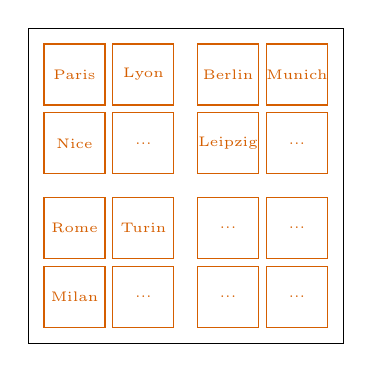
\begin{tikzpicture}	
			\draw [draw=black] (0, 0) rectangle (4,4) ;
			\draw [draw=orange] (0.2, 2.15) rectangle (0.975, 2.925) node[pos=.5] {\tiny \textcolor{orange}{Nice}};
			\draw [draw=orange] (1.075, 2.15) rectangle (1.85, 2.925) node[pos=.5] {\tiny \textcolor{orange}{...}};
			\draw [draw=orange] (0.2, 3.025) rectangle (0.975, 3.8) node[pos=.5] {\tiny \textcolor{orange}{Paris}};
			\draw [draw=orange] (1.075, 3.025) rectangle (1.85, 3.8) node[pos=.5] {\tiny \textcolor{orange}{Lyon}};
			\draw [draw=orange] (0.2, 0.2) rectangle (0.975, 0.975) node[pos=.5] {\tiny \textcolor{orange}{Milan}};
			\draw [draw=orange] (1.075, 0.2) rectangle (1.85, 0.975) node[pos=.5] {\tiny \textcolor{orange}{...}};
			\draw [draw=orange] (0.2, 1.075) rectangle (0.975, 1.85) node[pos=.5] {\tiny \textcolor{orange}{Rome}};
			\draw [draw=orange] (1.075, 1.075) rectangle (1.85, 1.85) node[pos=.5] {\tiny \textcolor{orange}{Turin}};
			
			\draw [draw=orange] (2.15, 0.2) rectangle (2.925, 0.975) node[pos=.5] {\tiny \textcolor{orange}{...}};
			\draw [draw=orange] (3.025, 0.2) rectangle (3.8, 0.975) node[pos=.5] {\tiny \textcolor{orange}{...}};
			\draw [draw=orange] (2.15, 1.075) rectangle (2.925, 1.85) node[pos=.5] {\tiny \textcolor{orange}{...}};
			\draw [draw=orange] (3.025, 1.075) rectangle (3.8, 1.85) node[pos=.5] {\tiny \textcolor{orange}{...}};
			
			\draw [draw=orange] (2.15, 2.15) rectangle (2.925, 2.925) node[pos=.5] {\tiny \textcolor{orange}{Leipzig}};
			\draw [draw=orange] (3.025, 2.15) rectangle (3.8, 2.925) node[pos=.5] {\tiny \textcolor{orange}{...}};
			\draw [draw=orange] (2.15, 3.025) rectangle (2.925, 3.8) node[pos=.5] {\tiny \textcolor{orange}{Berlin}};
			\draw [draw=orange] (3.025, 3.025) rectangle (3.8, 3.8) node[pos=.5] {\tiny \textcolor{orange}{Munich}};
		\end{tikzpicture}}
		\caption{By-city partition associated with (\ref{ex2:city-partition}). Cells are ordered on a grid for clarity only.}\label{fig2:city-partition}
	\end{subfigure}\hfill
	\begin{subfigure}[t]{.48\linewidth}
		\centering
		\scalebox{1.25}{
		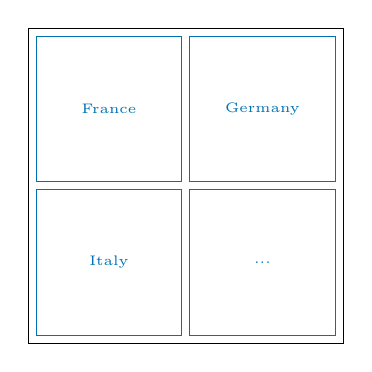
\begin{tikzpicture}	
			\draw [draw=black] (0, 0) rectangle (4,4);
			\draw [draw=blue] (0.1, 2.05) rectangle (1.95, 3.9) node[pos=.5] {\tiny \textcolor{blue}{France}};
			\draw [draw=blue] (2.05, 0.1) rectangle (3.9, 1.95) node[pos=.5] {\tiny \textcolor{blue}{...}};
			\draw [draw=blue] (0.1, 0.1) rectangle (1.95, 1.95) node[pos=.5] {\tiny \textcolor{blue}{Italy}};
			\draw [draw=blue] (2.05, 2.05) rectangle (3.9, 3.9) node[pos=.5] {\tiny \textcolor{blue}{Germany}};
		\end{tikzpicture}}
		\caption{By-country partition associated with (\ref{ex2:country-partition}). Cells are ordered on a grid for clarity only.}\label{fig2:country-partition}
	\end{subfigure}
	\caption{Standard partitions induced by a fine-grained (\ref{ex2:city-partition}) and a coarser-grained question (\ref{ex2:country-partition}).}
\end{figure}

Intuitively, grouping together the propositions listed in (\ref{ex2:city-partition}) talking about cities belonging to the same country, would help capture the desired property. This is done in (\ref{ex2:city-parse}). (\ref{ex2:city-parse}) then defines a set of sets of propositions. 
\begin{exe}
	\ex {$\llbracket$ In which city did Jo grow up?$\rrbracket^w$ =\\$\lbrace\lbrace p \ | \ \exists l. \ \text{$l$ is a city in $l'$} \wedge \ p = \lambda w'. \ \text{Jo grew up in $l$ in $w'$}\rbrace \ | \ l' \text{ is a country} \rbrace$}\label{ex2:city-parse}
\end{exe}

Grouping together cells within bigger sets (which are cells themselves), amounts to building a \textit{nested} partition of the CS. In our example, the ``outer'' partition is by-country, and the ``inner'' partition, is by-city. Graphically, this is equivalent to adding the ``blue rectangles'' from Figure \ref{fig2:country-partition}, to Figure \ref{fig2:city-partition}. This operation is performed in Figure \ref{fig2:city-recursive-partition}. The tree in Figure \ref{fig2:city-tree} is yet another, more readable way to represent the same thing. In this tree, each node refers to a proposition of the form \textit{Jo grew up in l}, $l$ denoting a city or a country. Each node is understood as intersected with the CS, which corresponds to the root of the tree. Therefore, each node forms a proper subset of the CS. Nodes appearing at the same level (forming a ``layer''), partition the CS. Deeper layers, correspond to finer-grained partitions. Tree like Figure \ref{fig2:city-tree} will be used throughout the dissertation to represent nested partitions like Figure \ref{fig2:city-recursive-partition}. One must always keep in mind that the two representations are equivalent. (\ref{ex2:set-tree-bijection}) formally defines the bijective mapping between nested sets of propositions (dubbed \textit{inductive propositions}) like (\ref{ex2:city-parse}), and tree structures like Figure \ref{fig2:city-tree}.

\begin{figure}[H]
	\centering
	\begin{subfigure}[t]{.45\linewidth}
		\centering
		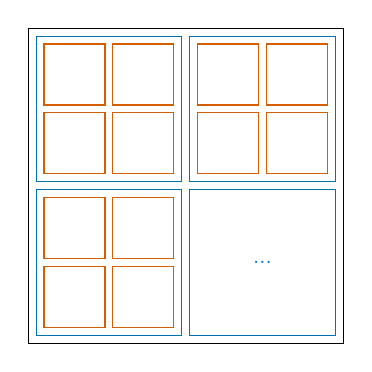
\begin{tikzpicture}	
			\draw [draw=black] (0, 0) rectangle (4,4) ;
			\draw [draw=blue] (0.1, 2.05) rectangle (1.95, 3.9);
				\draw [draw=orange] (0.2, 2.15) rectangle (0.975, 2.925);
				\draw [draw=orange] (1.075, 2.15) rectangle (1.85, 2.925);
				\draw [draw=orange] (0.2, 3.025) rectangle (0.975, 3.8);
				\draw [draw=orange] (1.075, 3.025) rectangle (1.85, 3.8);
			\draw [draw=blue] (2.05, 0.1) rectangle (3.9, 1.95) node[pos=.5] {\scriptsize \textcolor{blue}{...}};
			\draw [draw=blue] (0.1, 0.1) rectangle (1.95, 1.95);
				\draw [draw=orange] (0.2, 0.2) rectangle (0.975, 0.975);
				\draw [draw=orange] (1.075, 0.2) rectangle (1.85, 0.975);
				\draw [draw=orange] (0.2, 1.075) rectangle (0.975, 1.85);
				\draw [draw=orange] (1.075, 1.075) rectangle (1.85, 1.85);
			\draw [draw=blue] (2.05, 2.05) rectangle (3.9, 3.9);
				\draw [draw=orange] (2.15, 2.15) rectangle (2.925, 2.925);
				\draw [draw=orange] (3.025, 2.15) rectangle (3.8, 2.925);
				\draw [draw=orange] (2.15, 3.025) rectangle (2.925, 3.8);
				\draw [draw=orange] (3.025, 3.025) rectangle (3.8, 3.8);
		\end{tikzpicture}
		\caption{Recursive partition view}\label{fig2:city-recursive-partition}
	\end{subfigure}
	\hfill
	\begin{subfigure}[t]{.5\linewidth}
		\centering
		\vspace{-4.4cm}
		\begin{forest}
			[{CS\\
				Jo grew up in...}[\textcolor{blue}{France}[\textcolor{orange}{{Paris}}][\textcolor{orange}{Lyon}][\textcolor{orange}{...}]][\textcolor{blue}{Germany}[\textcolor{orange}{Berlin}][\textcolor{orange}{...}]][\textcolor{blue}{Italy}[\textcolor{orange}{...}]][\textcolor{blue}{...}]]
		\end{forest}
		\caption{Tree view}\label{fig2:city-tree}
	\end{subfigure}
	\caption{Alternative representations of the CS corresponding to the nested sets of (\ref{ex2:city-parse}).}\label{tree:country-city-parse}
\end{figure}


\begin{exe}
	\ex {\textsc{\textbf{Set-to-tree bijection}}. To define this bijection, we first define inductive propositions, and their propositional content. $S$ is an inductive proposition if either:
		\begin{itemize}
			\item $S$ is a set of worlds (i.e. a proposition);
			\item $S$ is a set of inductive propositions.
		\end{itemize}
		The propositional content of an inductive proposition is then defined as:
		\begin{itemize}
			\item If $S$ is a proposition: $S$;
			\item If $S$ is a set of inductive propositions: the grand union of the propositional contents of $S$'s elements.
		\end{itemize}
		Any inductive proposition $S$ is in a bijection with a tree structure whose nodes are propositions, and defined as:
		\begin{itemize}
			\item If $S$ is a proposition: the tree node denoting $S$;
			\item If $S$ is a set of inductive propositions: the tree whose root denotes $S$'s propositional content, and whose children are the tree structures induced by each of $S$'s elements. 
	\end{itemize}}\label{ex2:set-tree-bijection}
\end{exe}

So far, we have shown that the standard view linking questions to partitions, fails to account for the intuition that questions differing in terms of specificity, stand in some kind of inclusion relation encoded in their structure. We proposed a way to cash out this intuition, by appealing to recursive partitions, that we represent as trees for clarity.


We now proceed to generalize these observations about the structure of questions. Building on \textcite{Buring2003,Riester2019,Onea2016,Ippolito2019,Zhang2022} (among others), we take questions to denote \textit{parse trees} of the CS, i.e. structures that hierarchically organize the worlds of the CS. Such trees (abbreviated \textbf{Qtrees}) are defined in (\ref{ex2:qtree-def}). 
%(\ref{ex2:parse-def}) provide a more general definition of a parse.\footnote{This slightly differs from the notion of parse defined for sentences for instance, in which linear precedence must be preserved.} 
\begin{exe}
	\ex {\textsc{\textbf{Structure of Question-trees} (Qtrees)}. Qtrees are rooted trees whose nodes are all subsets of the CS and s.t.:
		\begin{itemize}
			\item Their root generally\footnote{In the case of sentences carrying presuppositions, the root will be assumed to correspond to the intersection between the CS and the sentence's presupposition. In fact, the whole Qtree will be intersected with the presupposition. This will be put to use in Chapter \ref{chap:scalarity}. But the examples we will see before this, will all involve Qtree rooted in the CS.} refers to the CS;
			\item Any intermediate node is a proposition, which is partitioned by the set of its children.
		\end{itemize}
	}\label{ex2:qtree-def}
\end{exe}
%	\ex {\textit{Parse.} Let $S$ be a set. A parse of $S$ is a rooted tree whose nodes are subsets of $S$ and s.t.:
%		\begin{itemize}
%			\item The root is $S$;
%			\item Any intermediate node is partitioned by the set of its children.
%		\end{itemize}
%	}\label{ex2:parse-def}

A Qtree can be bijectively mapped to a nested partition of the CS as defined in (\ref{ex2:nested-partition}). Due to this equivalence, we will mostly use Qtrees in the rest of this dissertation.

\begin{exe}
	\ex {\textsc{\textbf{Nested partition}}. A nested partition $P$ of a set $S$ is a kind of inductive proposition, s.t.:
		\begin{itemize}
			\item If $P$ is a set of inductive propositions, then the propositional contents of $P$'s elements partition $P$'s propositional content. Additionally, $P$'s elements are nested partitions of their own propositional content. 
		\end{itemize}	
	}\label{ex2:nested-partition}
\end{exe}


Before investigating the interpretation and the structural properties of model of questions, the next Section covers a few core concepts from graph theory that will be useful in the rest of the Chapter and beyond.


\subsection{A brief refresher on graph theory (and a few useful concepts for Qtrees)}

(\ref{ex2:qtree-def}) defines Qtres as rooted trees. Linguists typically understand trees as relations between parent nodes and their children, along the lines of (\ref{ex2:recursive-interpretation}).

\begin{exe}
	\ex {\textsc{\textbf{Rooted tree}} (inductive version). A tree rooted in $N$ is either:
		\begin{itemize}
			\item $N$ (single, childless node);
			\item $N$, along with $N$'s children, which are all rooted trees.
	\end{itemize}}\label{ex2:tree-inductive}
\end{exe}

But we will see throughout this dissertation that it is also useful to see a tree as a specific kind of graph. We will first define graphs, then define trees as a subkind of graph, and lastly, show the importance of defining a root in such trees. The definition of a graph is given in (\ref{ex2:graph}). A graph is a way to represent a binary relation, which by default will be symmetric\footnote{\textit{Undirected} graphs, that we will simply call graphs, implement symmetric relations, while \textit{directed} graphs implement asymmetric relations.}. Elements in the domain of the relation are modeled as nodes, and unordered pairs of nodes are connected with an edge, iff they verify the relation. A graph therefore amounts to a set of nodes, and a set of edges between these nodes. This is illustrated in Figure \ref{fig2:basic-graph}.

\begin{exe}	
	\ex {\textsc{\textbf{Graph}}. A graph is defined by a set of nodes $\mathcal{N}$ and by a set of edges $\mathcal{E}$ between elements of $\mathcal{N}$. Edges are defined as unordered pairs of nodes: $\mathcal{E} \subseteq \lbrace \lbrace N_1, N_2\rbrace \ | \ (N_1, N_2) \in \mathcal{N}^2\rbrace$}\label{ex2:graph}
\end{exe}

\begin{figure}[H]
	\centering
	\begin{tikzpicture}
		\node[shape=circle,draw=black] (A) at (0,0) {A};
		\node[shape=circle,draw=black] (B) at (0,3) {B};
		\node[shape=circle,draw=black] (C) at (2.5,4) {C};
		\node[shape=circle,draw=black] (D) at (2.5,1) {D};
		\node[shape=circle,draw=black] (F) at (5,3) {F} ;
		\node[shape=circle,draw=black] (E) at (-2,2) {E} ;
		
		\path [-,color=orange] (A) edge node[left] {} (B);
		\path [-](B) edge node[left] {} (C);
		\path [-,color=orange](A) edge node[left] {} (D);
		\path [-](D) edge node[left] {} (C);
		\path [-,color=orange](D) edge node[right] {} (F);   
	\end{tikzpicture}
	\caption{A graph $G=(\mathcal{N}, \mathcal{E})$, with $\mathcal{N}=\lbrace A, B, C, D, E, F\rbrace$ and $\mathcal{E}=\lbrace \lbrace A, B\rbrace, \lbrace A, D\rbrace, \lbrace B, C\rbrace, \lbrace C, D\rbrace, \lbrace D, F\rbrace\rbrace$.}\label{fig2:basic-graph}
\end{figure}

This definition allows to define rooted trees as a kind of graph with a few extra properties: connectivity, acyclicity, and rootedness; see (\ref{ex2:rooted-tree}). We now unpack what these three extra properties mean for graphs. This will lead us to define a few useful concepts applying to trees, namely paths, ancestry, and depth.

\begin{exe}
	\ex {\textsc{\textbf{Rooted tree}} (graph version). A rooted tree is a graph that is connected and acyclic, and features a distinguished node called root.}\label{ex2:rooted-tree}
\end{exe}

In graphs, sequences of adjacent edges form paths. For instance, in Figure \ref{fig2:basic-graph}, the ordered sequence $[$\textcolor{orange}{$\lbrace A, B\rbrace$}, \textcolor{orange}{$\lbrace A, D\rbrace$}, \textcolor{orange}{$\lbrace D, F\rbrace$}$]$ forms a path, between node $A$ and node $F$. This is generalized in (\ref{ex2:graph-path}).

\begin{exe}
	\ex {\textsc{\textbf{Path}}. Let $G = (\mathcal{N}, \mathcal{E})$ be a graph. Let $(N_1, N_2) \in \mathcal{N}^2$ be two nodes of $G$. There is a path in $G$ between $N_1$ and $N_2$ (abbreviated $N_1 \stackrel{G}{\leadsto}  N_2$) iff $N_1$ and $N_2$ can be connected by a series of edges in $G$, i.e. $\exists (e_1, ... e_k) \in \mathcal{E}^k. \ N_1 \in e_1 \wedge N_2 \in e_k \wedge \forall i \in [1; k-1]. \  |e_i \cap e_{i+1}|  = 1$, where $|.|$ is the cardinality operator.}\label{ex2:graph-path}
\end{exe}

In Figure \ref{fig2:basic-graph}, it is easy to see that nodes $A$, $B$, $C$, $D$ and $F$ are all connected to each other by at least one path (in fact, infinitely many of them that cycle through these nodes). Node $E$ on the other hand, is isolated. So, Figure \ref{fig2:basic-graph} represents a graph that is \textit{not} connected. If $E$ were removed from the set of nodes, and the edges remained the same, the resulting graph would be connected. This concept of connectivity is generalized in (\ref{ex2:graph-connectivity}). If a graph is a tree, then, it is connected.
\begin{exe}
	\ex {\textsc{\textbf{Connectivity}}. Let $G = (\mathcal{N}, \mathcal{E})$ be a graph. $G$ is connected, iff there is a path in $G$ between any pair of nodes in $\mathcal{N}$, i.e. $\forall (N_1, N_2) \in \mathcal{N}^2. \ N_1 \stackrel{G}{\leadsto} N_2$.}\label{ex2:graph-connectivity}
\end{exe}

Another thing to note about Figure \ref{fig2:basic-graph}, is that nodes $A$, $B$, $C$, and $D$ form a ``cycle'', there is a path that starts at one of these nodes (e.g., $C$), and ends at this very same node, \textit{via} $B$, $A$, and $D$. Because of this cycle, there are infinitely many paths between $A$, $B$, $C$, and $D$, and also between each of these nodes, and $F$. Removing the edge between, say, $A$ and $B$, would break the cycle (yet, interestingly, maintain connectivity between $A$, $B$, $C$, and $D$). The resulting graph would be acyclic. The general definition of an acyclic graph, is given in (\ref{ex2:graph-acyclic}). If a graph is a tree, then, it is acyclic. Moreover, connectivity and acyclicity, are necessary and sufficient for a graph to be a tree.

\begin{exe}
	\ex {\textsc{\textbf{Acyclicity}}. Let $G = (\mathcal{N}, \mathcal{E})$ be a graph. $G$ is acyclic, iff no node $N$ of $\mathcal{N}$ is s.t. there is a path starting and ending at $N$ in $G$, i.e. $\neg\exists N \in \mathcal{N}. \ N \stackrel{G}{\leadsto} N$.}\label{ex2:graph-acyclic}
\end{exe}

We now have a definition of what kind of data structure a tree is. But why do we need  Qtrees to be ``rooted''? To understand why, let us go back to the tree in Figure \ref{fig2:city-tree}, repeated in Figure \ref{fig2:city-tree-repeated} below. The way this tree is represented on paper, is somehow misleading. Recall that, from the point of view of graph theory, a tree is just an undirected graph, with a few extra properties constraining its edges. If the tree represented in Figure \ref{fig2:city-tree-repeated} were not ``rooted'', nothing would prevent us from representing it in the form of Figure \ref{fig2:city-tree-france-root}: the nodes and edges are strictly the same, but in Figure \ref{fig2:city-tree-france-root}, \textit{France} ``appears'' to be the root of the tree, because visually, it is represented at the top. To avoid this confusion, the fact that the CS node should be ``at the top'' is made part of the representation of the tree -- which then becomes a \textit{rooted} tree. So, a rooted tree is just a tree, plus one distinguished node that serves as root.

\begin{figure}[H]
	\centering
	\begin{subfigure}[t]{.45\linewidth}
		\centering
		\begin{forest}
			[{CS\\
				Jo grew up in...}[\textcolor{blue}{France}[\textcolor{orange}{{Paris}}][\textcolor{orange}{Lyon}][\textcolor{orange}{...}]][\textcolor{blue}{Germany}[\textcolor{orange}{Berlin}][\textcolor{orange}{...}]][\textcolor{blue}{Italy}[\textcolor{orange}{...}]][\textcolor{blue}{...}]]
		\end{forest}
		\caption{The ``intuitive'' view, in which the CS appears at the top.}\label{fig2:city-tree-repeated}
	\end{subfigure}
	\hfill
	\begin{subfigure}[t]{.45\linewidth}
		\centering
		\begin{forest}
			[\textcolor{blue}{France}[\textcolor{orange}{Paris}][\textcolor{orange}{Lyon}][\textcolor{orange}{...}][CS[\textcolor{blue}{Germany}[\textcolor{orange}{Berlin}][\textcolor{orange}{...}]][\textcolor{blue}{Italy}[\textcolor{orange}{...}]][\textcolor{blue}{...}]]]
		\end{forest}
		\caption{An alternative ``counter-intuitive'' view, in which the CS is \textit{not} at the top, yet all edges and nodes are the same.}\label{fig2:city-tree-france-root}
	\end{subfigure}
	\caption{Two equivalent ways to represent the tree corresponding to the question in (\ref{ex2:city-question}); assuming trees were connected, acyclic graphs, but not rooted.}
\end{figure}


The notion of a distinguished root in fact allows to define a few interesting properties on trees that linguist may be more familiar with, and that will be used throughout this dissertation. First, once a tree is rooted, it is possible to define a measure of distance between each node of the tree, and the root. This corresponds to the concept of depth, defined in (\ref{ex2:tree-node-depth}). In Figure \ref{fig2:city-tree-repeated} for instance, the CS has depth $0$, \textit{Germany} depth $1$, and \textit{Lyon} depth $2$. This also allows to define the global ``size'' of the tree, in the form of its maximal depth; see (\ref{ex2:tree-depth}). Figure \ref{fig2:city-tree-repeated} for instance, is a tree of depth $2$.

\begin{exe}
	\ex
	\begin{xlist}	
		\ex {\textsc{\textbf{Depth of a node in a rooted tree}}. Let $T = (\mathcal{N}, \mathcal{E}, R)$ be a rooted tree, with root $R$. Let $N \in \mathcal{N}$. The depth of $N$ in $T$ ($d(N, T)$) corresponds to the length of the minimal path between $R$ and $N$ if $N \neq R$,\footnote{This path can be determined using a simple Depth-First Search algorithm starting from the root.} and is set to $0$ if $N = R$.}\label{ex2:tree-node-depth}
		\ex {\textsc{\textbf{Depth of a rooted tree}}. Let $T = (\mathcal{N}, \mathcal{E}, R)$ be a rooted tree, with root $R$. The depth of $T$ ($d(T)$) is the maximal depth of a node in $T$: $d(T) = max_{N \in \mathcal{N}}(d(N, T))$.}\label{ex2:tree-depth}
	\end{xlist}
\end{exe}

Having a distinguished root, and the derived concepts of depth, gives us the parent-child relation between nodes for free.\footnote{in the next Section, we will introduce another definition of tree, that takes this relation as a primitive} This relation is defined based on depth and edges in (\ref{ex2:parent-child}), and its transitive closure (the ancestor relation) is defined in (\ref{ex2:ancestor}), in two possible ways. 

\begin{exe}
	\ex {\textsc{\textbf{Parent-child relation in a rooted tree}}. Let $T = (\mathcal{N}, \mathcal{E}, R)$ be a rooted tree. Let $(N_1, N_2) \in \mathcal{N}^2$. $N_1$ is the parent of $N_2$  (and $N_2$ is the child of $N_1$), iff $\lbrace N_1, N_2\rbrace \in \mathcal{E}$ and $d(N_1, T) < d(N_2, T)$.}\label{ex2:parent-child}
	\ex\label{ex2:ancestor}
	\begin{xlist}
		\ex {\textsc{\textbf{Ancestor relation}} (recursive version). Let $T = (\mathcal{N}, \mathcal{E}, R)$ be a rooted tree. Let $(N_1, N_2) \in \mathcal{N}^2$. $N_1$ is an ancestor of $N_2$ iff either:
			\begin{itemize}
				\item $N_1$ is the parent of $N_2$;
				\item or $N_1$ is the parent of an ancestor of $N_2$.
		\end{itemize}}
	\ex {\textsc{\textbf{Ancestor relation}} (path version). Let $T = (\mathcal{N}, \mathcal{E}, R)$ be a rooted tree. Let $(N_1, N_2) \in \mathcal{N}^2$. $N_1$ is an ancestor of $N_2$ iff $N_1 \stackrel{T}{\leadsto} N_2$ and $d(N_1, T) < d(N_2, T)$.}
	\end{xlist}
\end{exe}

Lastly, in the rest of this dissertation, we will extensively use the concept of \textit{layer}, that we define as a the maximal set of same-depth nodes in a rooted tree; see (\ref{ex2:tree-layer}). Figure \ref{fig2:city-tree-repeated} features a country-layer at depth $1$, and a city-layer at depth $2$. Layers therefore reflect an intuitive notion of granularity.

\begin{exe}
	\ex {\textsc{\textbf{Depth-$k$ layer of a rooted tree}}. Let $T = (\mathcal{N}, \mathcal{E}, R)$ be a rooted tree, with root $R$. Let $k$ be an integer s.t. $0\geq k<d(T)$. The depth-$k$ layer of $T$ is the set of nodes in $\mathcal{N}$ whose depth is $k$, i.e. $\lbrace N \in \mathcal{N} \ | \ d(N, T)=k\rbrace$.}\label{ex2:tree-layer}
\end{exe}


Now that we have defined the core structure of Qtrees along with a few related properties and metrics, we proceed to assign an interpretation to this kind of structure.

\subsection{Interpreting Qtrees}\label{sec:interpreting-qtrees}
\cite{Aloni2022}
At the end of Section \ref{sec:nested-partition}, we showed that question should better be represented as nested partition, in order to encode their degree of specificity, and the grammar sensitive to how more or less fine-grained questions relate to each other. We also discussed how nested partitions could be unequivocally represented as Qtrees. It is easy to see that the tree in Figure \ref{fig2:city-tree}/\ref{fig2:city-tree-repeated}, repeated again in Figure \ref{fig2:city-qtree}, is a Qtree according to (\ref{ex2:qtree-def}). We saw that this Qtree intuitively capture the idea that a \textit{Which country?} kind of question, is contained in a \textit{Which city?} kind of question. We now investigate how to exploit this hierarchy in a meaningful way. We will use Figure \ref{fig2:city-qtree} as an example, and now assign an interpretation to nodes and paths in such structures. We will focus on three meaningful aspects of Qtrees: answer-granularity (understood as node depth), strategies of inquiry (understood as paths), and question refinement (understood as tree inclusion)

\begin{figure}[H]
	\centering
	\begin{forest}
		[{CS\\
			Jo grew up in...}[\textcolor{blue}{France}[\textcolor{orange}{{Paris}}][\textcolor{orange}{Lyon}][\textcolor{orange}{...}]][\textcolor{blue}{Germany}[\textcolor{orange}{Berlin}][\textcolor{orange}{...}]][\textcolor{blue}{Italy}[\textcolor{orange}{...}]][\textcolor{blue}{...}]]
	\end{forest}
	\caption{``Intuitive'' Qtree for \textit{Which city did Jo grow up in?}}\label{fig2:city-qtree}
\end{figure}

We start with the interpretation of nodes as possible answers, with different granularities. The root of Figure \ref{fig2:city-qtree} for instance, which corresponds to the entire CS, defines a tautology: it is a proposition which is true of all worlds of the CS, because it simply coincides with it.\footnote{Chapter \ref{chap:introduction} moreover identifies it as an uninformative proposition that is Lewis-relevant but not Roberts-relevant.} It can be understood as identifying the unique cell of coarsest-grained partition of the CS, that is, the CS itself. By contrast, leaves like \textit{Paris}, \textit{Lyon}, \textit{Berlin} in Figure \ref{fig2:city-qtree}, correspond to the ``smallest'' cells of the recursive partition that the Qtree defines. They can be seen as maximal answer to the underlying question, e.g., \textit{In which city did Jo grow up?}. Intermediate nodes like \textit{France} or \textit{Germany} in Figure \ref{fig2:city-qtree}, form cells of ``intermediate'' size, and can always be seen as unions of leaves. They appear to correspond to non-maximal answers. Because Qtrees can be made of many layers, they induce a hierarchy between non-maximal answers: an non-maximal answer $p$ is ``more maximal'' than another non-maximal answer $q$, iff the node corresponding to $p$ is located deeper in the Qtree than the node corresponding to $q$. This is formalized in (\ref{ex2:answer-gran}).

\begin{exe}
	\ex {\textsc{\textbf{Answer granularity}}. Let $T$ be a Qtree and $(N_1, N_2)$ be two nodes in $T$. $N_1$ constitutes a finer-grained answer than $N_2$ iff $d(N_1, T) > d(N_2, T)$. This implies that leaves of $T$ correspond to the finest-grained answers (maximal answers) to the question $T$ represents.}\label{ex2:answer-gran}
\end{exe}


Next, we discuss how Qtree encapsulate \citeauthor{Roberts1996}'s notion of \textit{Strategy of Inquiry}. To this end, we observe that nodes in a tree can receive a ``recursive'' interpretation, that incorporates everything the node dominates. Under this interpretation, a node $N$ in a Qtree is not only what $N$ denotes; it is the whole subtree ($\sim$subquestion) rooted in $N$, as defined in (\ref{ex2:recursive-interpretation})


\begin{exe}
	\ex\label{ex2:recursive-interpretation} {\textsc{\textbf{Recursive interpretation of tree nodes}}. Let $T = (\mathcal{N}, \mathcal{E}, R)$ be a rooted tree. Let $N \in \mathcal{N}$ be a node of $T$. $N$'s recursive interpretation corresponds to:
		\begin{itemize}
			\item $N$, if $N$ is a leaf;
			\item the subtree of $T$ rooted in $N$, otherwise. 
	\end{itemize}}
\end{exe}

This point of view originates from the inductive definition of a rooted tree given in (\ref{ex2:tree-inductive}) and repeated below.

\begin{exe}
	\exr{ex2:tree-inductive} {\textsc{\textbf{Rooted tree}} (inductive version). A tree rooted in $N$ is either:
		\begin{itemize}
			\item $N$ (single, childless node);
			\item $N$, along with $N$'s children, which are all rooted trees.
	\end{itemize}}
\end{exe}

If $T$ is a Qtree, then $N$'s recursive interpretation will be the Qtree rooted in $N$. This Qtree's root can be seen as a ``local'' CS, which is equal to the global CS, updated with $N$. For instance, the recursive interpretation of the \textit{France}-node in Figure \ref{fig2:city-qtree}, corresponds to the subtree of Figure \ref{fig2:city-qtree} rooted in \textit{France}. This subtree, given in Figure \ref{fig2:france-subtree}, amounts to the question \textit{In which city did Jo grow up?}, granted that \textit{Jo lives in France}, since its root corresponds to the CS intersected with the proposition that \textit{Jo lives in France}.

\begin{figure}[H]
	\centering
	\begin{forest}
		[\textcolor{blue}{France}[\textcolor{orange}{{Paris}}][\textcolor{orange}{Lyon}][\textcolor{orange}{...}]]
	\end{forest}
	\caption{``Recursive'' interpretation of the \textit{France}-node in Figure \ref{fig2:city-qtree}.}\label{fig2:france-subtree}
\end{figure}

In fact, this subtree as a whole, can be understood as the tree-node intersection of Figure \ref{fig2:city-qtree} and the proposition that \textit{Jo grew up in France}. Tree-node intersection is defined in (\ref{ex2:nodewise-inter}). This operation takes a Qtree and a proposition $p$, and creates a Qtree whose nodes are each intersected with $p$, and resulting empty nodes are removed. Edges from the original Qtree are retained, as long as the nodes they connect are still part of the newly formed Qtree. Note that, because the nodes and edges of a tree form \textit{sets} (and not \textit{multisets}), tree-node intersection automatically collapses nodes from the original tree whose intersections with $p$ yield the same result; and it also collapses the edges between such nodes. Figure \ref{fig2:tree-node-inter} provides a decomposition of this procedure, computing the tree-node intersection between Figure \ref{fig2:city-qtree} and the proposition that \textit{Jo grew up in France}, and illustrating how nodes and edges may ``collapse''. (\ref{ex2:recursive-interpretation-cs}) generalizes this point, by stating that the subtree of a Qtree rooted in a node $N$, can be reconstructed by tree-node intersecting the entire Qtree with the proposition $N$ corresponds to. In other words, the subquestion corresponding to a node $N$, can be seen as a \textit{restriction} of the entire Qtree, taking $N$ for granted. This is proved in (\ref{ex2:recursive-interpretation-cs-proof}).

\begin{exe}
	\ex {\textsc{\textbf{Tree-node Intersection}}. Let $T=(\mathcal{N}, \mathcal{E}, R)$ be a Qtree. Let $p$ be a proposition. The tree-node intersection between $T$ and $p$, noted $T \cap p$, is defined iff $R \cap p \neq \emptyset$ and, if so, is the Qtree $T'=(\mathcal{N}', \mathcal{E}', R')$ s.t.:
	\begin{itemize}
		\item $\mathcal{N}' = \lbrace N \cap p \ | \ N \in \mathcal{N} \wedge N \cap p \neq \emptyset\rbrace$
		\item $\mathcal{E}' = \lbrace \lbrace N_1\cap p, N_2\cap p\rbrace \ | \ \lbrace N_1, N_2\rbrace \in \mathcal{E} \wedge (N_1\cap p) \neq (N_2\cap p) \wedge N_1\cap p \neq \emptyset \wedge N_2\cap p \neq \emptyset \rbrace$
		\item $R' = R\cap p$
		\end{itemize}}\label{ex2:nodewise-inter}
\end{exe}

\begin{figure}[H]
	\centering
	\begin{subfigure}[t]{\linewidth}
		\centering
		\scalebox{.8}{
			\begin{forest}
				[{CS $\cap$ \textcolor{blue}{France}}[{\textcolor{blue}{France} $\cap$ \textcolor{blue}{France}}[{\textcolor{orange}{{Paris}} $\cap$ \textcolor{blue}{France}}][{\textcolor{orange}{Lyon} $\cap$ \textcolor{blue}{France}}][\textcolor{orange}{...}]][{\textcolor{blue}{Germany} $\cap$ \textcolor{blue}{France}}[{\textcolor{orange}{Berlin} $\cap$ \textcolor{blue}{France}}][\textcolor{orange}{...}]][{\textcolor{blue}{Italy} $\cap$ \textcolor{blue}{France}}[\textcolor{orange}{...}]][\textcolor{blue}{...}]]
			\end{forest}
		}
		\caption{Intersecting the tree in Figure \ref{fig2:city-qtree} with the proposition that \textit{Jo grew up in France}.}
	\end{subfigure}
	
	\begin{subfigure}[t]{.33\linewidth}
		\centering		\scalebox{.8}{
		\begin{forest}
			[{\textcolor{blue}{France}}[\textcolor{blue}{France}[\textcolor{orange}{{Paris}}][\textcolor{orange}{Lyon}][\textcolor{orange}{...}]][$\emptyset$[$\emptyset$][$\emptyset$]][$\emptyset$[$\emptyset$]][$\emptyset$]]
		\end{forest}}
		\caption{...After computing tree-node intersections.}
	\end{subfigure}
	\hfill
	\begin{subfigure}[t]{.27\linewidth}
		\centering		\scalebox{.8}{
		\begin{forest}
			[\textcolor{blue}{France}[\textcolor{blue}{France}[\textcolor{orange}{{Paris}}][\textcolor{orange}{Lyon}][\textcolor{orange}{...}]]]
		\end{forest}}
		\caption{...After removing empty nodes and resulting dangling edges.}
	\end{subfigure}
	\hfill
	\begin{subfigure}[t]{.3\linewidth}
		\centering 		\scalebox{.8}{
		\begin{forest}
			[\textcolor{blue}{France}[\textcolor{orange}{{Paris}}][\textcolor{orange}{Lyon}][\textcolor{orange}{...}]]
		\end{forest}}
		\caption{...After removing trivial edges: we get Figure \ref{fig2:france-subtree} back.}
	\end{subfigure}
	\caption{The recursive interpretation of a node, can be obtained by intersecting the whole Qtree with that node, removing empty nodes and trivial edges (formed by a parent node and its only child).}\label{fig2:tree-node-inter}
\end{figure}

\begin{exe}
 	\ex {\textsc{\textbf{Recursive interpretation and CS update}}. Let $T$ be a Qtree. Let $N$ be a node of $T$. $N$'s recursive interpretation corresponds to the tree-node intersection of $T$ with $N$.}\label{ex2:recursive-interpretation-cs}
 	\ex {\textsc{\textbf{Proof of (\ref{ex2:recursive-interpretation-cs})}}. Let $T$ be a Qtree. Let $N$ be a node of $T$. Because $T$ is a Qtree, any node $N$ dominates is a subset of $N$; any node dominating $N$, is a superset of $N$, and any node that is neither dominated nor dominating $N$, is disjoint from $N$. By definition, $N$'s recursive interpretation is the subtree of $T$ rooted in $N$, noted $T'$. We show that $T'$ corresponds to the tree-node intersection between $T$ and $N$, $T \cap N$. Let $N'$ be $N$ or a node dominated by $N$. $N' \subseteq N$, so $N' \cap N = N'$. This holds for any $N'$ dominated by $N$ or equal to $N$. So $T \cap N$ preserves $T'$. Let $N'$ be an ancestor of $N$. $N \subseteq N'$ so $N' \cap N = N$. So any ancestor of $N$ in $T$, is reduced to $N$ in $T \cap N$. Let $N'$ be a node in $T$ that is neither dominated nor dominating $N$. $N \cap N' = \emptyset$, and so any sibling/uncle/cousin of $N$ in $T$ is absent in $T \cap N$, along with any incident edges. Therefore, $T \cap N$ ends up being just $T'$.}\label{ex2:recursive-interpretation-cs-proof}
\end{exe}

We have just seen that under the recursive interpretation of nodes, each node $N$ can be seen as a subquestion of the whole Qtree, which takes $N$'s propositional content for granted. Under this interpretation, a path from the root (CS) to any node $N$, can then be seen as a series of subquestions, taking for granted increasingly strong propositions. In Figure \ref{fig2:city-qtree} for instance, a path of the form $[\textit{CS}, \textit{France}, \textit{Paris}]$, can be interpreted as a series of inquiries of the form: $[$\textit{In which city did Jo grow up (I have no idea)?}, \textit{In which city did Jo grow up (given Jo grew up in France)?}, \textit{Jo grew up in Paris}$]$. If the path terminates on a leaf, then the series of inquiries converges to a maximal answer. We will call such paths complete strategies of inquiry.

\begin{exe}
	\ex {\textsc{\textbf{Complete Strategy of Inquiry}}. Let $T$ be a Qtree. A complete strategy of inquiry on $T$ is a path from $T$'s root to one of $T$'s leaves.}
\end{exe}

This model is very close to what the previous literature had posited at the conversational level, whereby sentences answer questions and sometimes evoke new, finer-grained questions. The key difference here, is that individual questions are assumed to encapsulate the same kind of dynamic, hierarchical information. How does this relate to question granularity? Note that intuitively finer-grained questions yield deeper Qtrees than intuitively coarser-grained ones. Additionally, (\ref{ex2:tree-depth}) defined Qtree depth as the maximal length of a path from the root to a leaf in the tree. This leads to the equivalence in (\ref{ex2:depth-soi}).

\begin{exe}
	\ex {\textit{\textbf{Depth and Complete Strategies of Inquiry}}. Let $T$ be a Qtree. $T$'s depth can be recovered by finding the length of its longest complete strategy of inquiry, dubbed maximal complete strategy of inquiry.}\label{ex2:depth-soi}
\end{exe}

In other words, finer-grained questions are linked to deeper Qtrees, which are characterized by a longer, maximal complete strategy of inquiry. In sum, a fine-grained question is a question for which converging to a maximal answer may require a lot of intermediate steps, or subquestions. This is useful as an absolute measure of question-complexity, but probably not enough to determine if a question is finer-grained than another question. For instance, this incorrectly predicts two completely independent questions to be comparable in terms of granularity, just because they give rise to Qtree of different depths. 



There is in fact another way in which the recursive interpretation of nodes can help clarify in what sense a \textit{Which city} kind of question, is more fine-grained than a \textit{Which country} kind of question, in the current framework. Figure \ref{fig2:qtrees-diff-gran} shows what a Qtree for (\ref{ex2:city-partition}) and a Qtree for (\ref{ex2:country-partition}) should intuitively look like. 

\begin{figure}[H]
	\centering
	\begin{subfigure}[t]{.45\linewidth}
		\centering
		\begin{forest}
			[{CS\\
				Jo grew up in...}[\textcolor{blue}{France}[\textcolor{orange}{{Paris}}][\textcolor{orange}{Lyon}][\textcolor{orange}{...}]][\textcolor{blue}{Germany}[\textcolor{orange}{Berlin}][\textcolor{orange}{...}]][\textcolor{blue}{Italy}[\textcolor{orange}{...}]][\textcolor{blue}{...}]]
		\end{forest}
		\caption{``Intuitive'' Qtree for (\ref{ex2:city-partition}) = \textit{Which city did Jo grow up in?}}\label{fig2:city-qtree-repeated2}
	\end{subfigure}\hfill
	\begin{subfigure}[t]{.45\linewidth}
		\centering
		\begin{forest}
			[{CS\\
				Jo grew up in...}[\textcolor{blue}{France}][\textcolor{blue}{Germany}][\textcolor{blue}{Italy}][\textcolor{blue}{...}]]
		\end{forest}
		\caption{``Intuitive'' Qtree for (\ref{ex2:country-partition}) = \textit{Which country did Jo grow up in?}}\label{fig2:country-qtree}
	\end{subfigure}
	\caption{Comparing \textit{Which city} and \textit{Which country} Qtrees.}\label{fig2:qtrees-diff-gran}
\end{figure}
The Qtree for (\ref{ex2:city-partition}) stops at the city-level, because cities should constitute maximal answer to that kind of question; the Qtree for (\ref{ex2:country-partition}) on the other hand, stops at the country level, for similar reasons. And it is easy to notice that the Qtree for (\ref{ex2:country-partition}) somehow forms a ``subset'' of the Qtree for (\ref{ex2:city-partition}): it forms a subset of the nodes, and a subsets of the edges, of the Qtree for (\ref{ex2:city-partition}). Additionally, it is not a random subgraph of Figure \ref{fig2:city-qtree-repeated2} (as defined in (\ref{ex2:subgraph})). It remains a Qtree, that constitues a refinement of Figure \ref{fig2:city-qtree-repeated2}, as defined in (\ref{ex2:qtree-refinement}). It can also be shown, that all the possible refinements of a Qtree $T$, correspond to all the possible subgraphs of $T$ that have the Qtree property.\footnote{We identify the refinement operation between $T$ and $T'$, as a set $\mathcal{T}$ of subtrees of $T$, that is closed under root-sisterhood.
	We assume $T$ is a refinement of a Qtree $T'$ and show $T'$ is a subgraph of $T$ with the Qtree property. $T'$ is obtained from $T$ by removing the subtrees in $\mathcal{T}$ from $T$. So it is obviously a subgraph of $T$. We now show $T'$ is a Qtree. $\mathcal{T}$ cannot contain the tree rooted in $T$, otherwise $T'$ would be empty. So $T'$ has same root as $T$, and this root is the CS. Let $N$ be an intermediate node in $T'$. $N$ has at least one child $N'$, which means that $\mathcal{T}$ cannot contain the subtree of $T$ rooted in $N'$. To be partitioned by its children, $N$ in $T'$ must have the same children as $N$ in $T$, i.e. $\mathcal{T}$ should not contain any tree rooted in a child of $N$. If $\mathcal{T}$ did, then $\mathcal{T}$ would also contain the subtree of $T$ rooted in $N'$, du to its closure property. Contradiction. So $N$ retained all its children from $T$, and is partitioned by them, given that $T$ is a Qtree.\\
	We assume $T'$ is a subgraph of $T$ with the Qtree property and show $T$ is a refinement of a Qtree $T'$. $T'$ is a subgraph of $T$, so we can define $S$ the set of nodes of $T$ not in $T'$. We then define $\mathcal{T}$ as the set of subtrees of $T$ rooted in a maximal element of $S$ w.r.t. the ancestor relation, as induced by $T$'s edges. We show this set is closed under root-sisterhood. Let $T'' \in \mathcal{T}$. It is subtree of $T$ rooted in some node $N$, and $N$ is maximal in $S$ w.r.t. the ancestor relation. If $N$ has no sister in $T$, then the closure property is trivially verified. If $N$ has a sister $N'$ in $T$, we show the closure property by contradiction. If the subtree of $T$ rooted in $N'$ did not belong to $\mathcal{T}$, then, either $N'$ would be part of a subtree of $\mathcal{T}$ (but not as root), or, $N'$ would be a node in $T'$. The former option would imply that some common ancestor of $N$ and $N'$ would be the root of a subtree in $\mathcal{T}$. But then both $N$ and some ancestor of $N$, would be maximal in $S$ w.r.t. the ancestor relation. Contradiction. The former option would mean that $N'$'s parent in $T'$, would have $N'$, but not $N$ has child, and so would not be partitioned by its children. Therefore, $T'$ would not be a Qtree. Contradiction.}

\begin{exe}
	\ex {\textit{\textbf{Subgraph}}. Let $G = (\mathcal{N}, \mathcal{E})$ and $G' = (\mathcal{N}', \mathcal{E}')$ be two graphs. $G' \subseteq G$, iff $\mathcal{N}' \subseteq \mathcal{N}$ and $\mathcal{E}' \subseteq \mathcal{E}$.}\label{ex2:subgraph}
	\ex {\textit{\textbf{Qtree refinement}}. Let $T$ and $T'$ be Qtrees. $T$ is a refinement of $T'$ (or: $T$ is finer-grained than $T'$), iff $T'$ can be obtained from $T$ by removing a subset $\mathcal{T}$ of $T$'s subtrees, s.t., if $\mathcal{T}$ contains a subtree rooted in $N$, then, for each node $N'$ that is a sibling of $N$ in $T$, the subtree of $T$ rooted in $N'$, is also in $\mathcal{T}$.}\label{ex2:qtree-refinement}
\end{exe}


Two other possible refinements of Figure \ref{fig2:city-qtree-repeated2} are given below. It is worth noting that the process deriving a refinement from a Qtree need not remove entire layers. 



\begin{figure}[H]
	\centering
	\begin{subfigure}[t]{.45\linewidth}
		\centering
		\begin{forest}
			[{CS\\
				Jo grew up in...}[\textcolor{blue}{France}[\textcolor{orange}{Paris}][\textcolor{orange}{Lyon}][\textcolor{orange}{...}]][\textcolor{blue}{Germany}][\textcolor{blue}{Italy}[\textcolor{orange}{...}]][\textcolor{blue}{...}]]
		\end{forest}
		\caption{A refinement where the children of the \textit{Germany}-node are deleted.}\label{fig2:city-qtree-trimmed1}
	\end{subfigure}\hfill
	\begin{subfigure}[t]{.45\linewidth}
		\centering
		\begin{forest}
			[{CS\\
				Jo grew up in...}[\textcolor{blue}{France}][\textcolor{blue}{Germany} [\textcolor{orange}{Berlin}][\textcolor{orange}{...}]][\textcolor{blue}{Italy}[\textcolor{orange}{...}]][\textcolor{blue}{...}]]
		\end{forest}
		\caption{A refinement where the children of the \textit{France}-node are deleted.}\label{fig2:city-qtree-trimmed2}
	\end{subfigure}
	\caption{Possible refinements of the Qtree for \textit{Which city did Jo grow up in?} in Figure \ref{fig2:city-qtree-repeated2}.}\label{fig2:qtrees-trimmed}
\end{figure}




\subsection{Flagging Qtrees}

So far, we have considered Qtrees directly associated with questions, like (\ref{ex2:city-question}) and (\ref{ex2:country-question}). But, as suggested in the introduction to this Chapter, we want to go one step further, and posit that assertive sentences, like (\ref{ex2:city-assertion}) and (\ref{ex2:country-assertion}), also evoke questions in the form of Qtrees. Such questions will correspond to the ones a given assertion could be a good answer to.

\begin{exe}
	\ex \label{ex2:city-country-assertions}
	\begin{xlist}
		\ex {Jo grew up in Paris.}\label{ex2:city-assertion}
		\ex {Jo grew up in France.}\label{ex2:country-assertion}
	\end{xlist}
\end{exe}

So (\ref{ex2:city-assertion}) and (\ref{ex2:country-assertion}) for instance, should evoke Qtrees associated with questions like (\ref{ex2:city-question}) and (\ref{ex2:country-question}), respectively. We sketched an intuitive representation of these Qtrees in Figure \ref{fig2:qtrees-diff-gran}. Are these Qtrees representing everything that the assertions in (\ref{ex2:city-assertion}) and (\ref{ex2:country-assertion}) convey though? One major difference between questions and assertions, is that questions are ignorant of the answer, while assertions provide such an answer. So, if (\ref{ex2:city-assertion}) were directly mapped to the Qtree in Figure \ref{fig2:city-qtree-repeated2}, the information that (\ref{ex2:city-assertion}) actually answers the question by identifying the \textit{Paris}-node, would be lost. Another way to see the issue, is to observe that (\ref{ex2:city-assertion}) and (\ref{ex2:city-assertion2}) would then be associated with the exact same Qtree.

\begin{exe}
	\ex {Jo grew up in Berlin.}\label{ex2:city-assertion2}
\end{exe}

To avoid such collisions in the case of assertive sentences, we define an extra piece of machinery on top of the Qtree architecture, that consists in a set of ``verifying'' nodes keeping track of \textit{how} the assertion answers the question it evokes. I Figures, these nodes will be represented in boxes; given a Qtree $T$, $T$'s set of verifying nodes will be referred to as $\mathcal{N}^+(T)$. (\ref{ex2:city-assertion}) and (\ref{ex2:country-assertion}) for instance, will intuitively evoke Qtree that \textit{structurally} match those in Figure \ref{fig2:qtrees-diff-gran}, but whose \textit{Paris} and \textit{France} noes respectively, are ``boxed'', i.e. flagged as verifying.

\begin{figure}[H]
	\centering
	\begin{subfigure}[t]{.45\linewidth}
		\centering
		\begin{forest}
			[{CS\\
				Jo grew up in...}[\textcolor{blue}{France}[\textcolor{orange}{{\fbox{Paris}}}][\textcolor{orange}{Lyon}][\textcolor{orange}{...}]][\textcolor{blue}{Germany}[\textcolor{orange}{Berlin}][\textcolor{orange}{...}]][\textcolor{blue}{Italy}[\textcolor{orange}{...}]][\textcolor{blue}{...}]]
		\end{forest}
		\caption{``Intuitive'' Qtree for (\ref{ex2:city-partition}) = \textit{Which city did Jo grow up in?}}\label{fig2:paris-qtree}
	\end{subfigure}\hfill
	\begin{subfigure}[t]{.45\linewidth}
		\centering
		\begin{forest}
			[{CS\\
				Jo grew up in...}[\textcolor{blue}{\fbox{France}}][\textcolor{blue}{Germany}][\textcolor{blue}{Italy}][\textcolor{blue}{...}]]
		\end{forest}
		\caption{``Intuitive'' Qtree for (\ref{ex2:country-partition}) = \textit{Which country did Jo grow up in?}}\label{fig2:france-qtree}
	\end{subfigure}
	\caption{Comparing \textit{Which city} and \textit{Which country} Qtrees.}\label{fig2:paris-france-qtrees}
\end{figure}

In that particular case, the nodes that are flagged as verifying in both Qtrees, strictly coincide with the proposition conveyed by the assertions, namely, that \textit{Jo grew up in Paris}, and that \textit{Jo grew up in France}. For an assertion like (\ref{ex2:city-assertion2}), the only flagged node would be \textit{Berlin}. But we will not take this strict equivalence between prejacent proposition and verifying nodes to be a generality. In the model laid out in the next Section, we will assume that verifying nodes, just like Qtree structure, are compositionally ``retro-engineered'' from the structure and meaning of the sentence. As a result, there may be more than on verifying node in a given Qtree, and, the grand union of a Qtree's verifying nodes, may not always coincide with the proposition denoted by the assertion.\footnote{This will in particular be true of conditional assertions.}
The next Section therefore introduces a more systematic way to derive Qtrees and their verifying nodes from simplex sentences.


Moreover, an accommodated Qtree should allow the sentence evoking it to properly answer it; that is why we assume that any well-formed Qtree derived from a sentence should come with a non-empty set of verifying nodes.(see (\ref{ex2:vacuous-flagging})). More generally, we assume that oddness results from the fact that a given sentence, through its LF, cannot give rise to any well-formed Qtree. This is summarized in (\ref{ex2:oddness-sentence}).


\begin{exe}
	\ex {\textit{\textbf{Empty labeling of verifying nodes}}. If a sentence $S$ evokes a Qtree $T$ but does not flag any node as verifying on $T$, then $T$ is deemed odd given $S$.}\label{ex2:vacuous-flagging}
	\ex {\textit{\textbf{Oddness of a sentence}}. A sentence $S$ is odd if any Qtree $T$ it evokes is odd given $S$.}\label{ex2:oddness-sentence}
\end{exe}



\section{Compositional Qtrees: base case}\label{sec:simplex}

So far, we have established that assertive sentences can evoke the questions they are good answers to, in the form of Qtrees. And we used ``intuitive'' Qtrees like the ones in Figures \ref{fig2:paris-qtree} and \ref{fig2:france-qtree} to show how such structures could capture a wide range of properties connecting questions and answers, and questions to each other. We now introduce a principled algorithm to derive Qtrees out of assertive sentences. This will heavily build on the notion of alternatives and how they can be ordered in terms of specificity. We will show that this ordering of alternatives induces a specific ``layering'' on Qtrees.

\subsection{Alternatives}

It is quite uncontroversial that assertive sentences evoke alternatives \parencite{Rooth1992,Katzir2007,Fox2011}. An alternative is a sentence that is sufficiently ``similar'' to the sentence it is evoked by, but may have a different meaning. For instance, (\ref{ex2:alt-some}) is felt to have (\ref{ex2:alt-all}) as alternative, and vice versa. Pre-theoretically, this is because, in many contexts, (\ref{ex2:alt-some}) is utterable iff (\ref{ex2:alt-all}) is, too. The same holds for (\ref{ex2:alt-paris}) and (\ref{ex2:alt-lyon}).

\begin{exe}
	\ex \label{ex2:alt-scalar}
	\begin{xlist}
		\ex {Jo ate all of the cookies.}\label{ex2:alt-some}
		\ex {Jo ate some of the cookies.}\label{ex2:alt-all}
	\end{xlist}
	\ex \label{ex2:alt-non-scalar}
	\begin{xlist}
		\ex {Jo grew up in Paris.}\label{ex2:alt-paris}
		\ex {Jo grew up in Lyon.}\label{ex2:alt-lyon}
	\end{xlist}
\end{exe}

Moreover, the computation of alternatives is driven by focus. In (\ref{ex2:alt-scalar}) and (\ref{ex2:alt-non-scalar}), it was implicitely assumed that quantifiers and city names respectively, were focused, and so gave rise to alternative varying in terms of the focused element. But note that, if the object of (\ref{ex2:alt-some}) and the verb of (\ref{ex2:alt-paris}) had been focused instead, the alternatives to these sentences would have been different, along the lines of (\ref{ex2:alt-muffins}) and (\ref{ex2:alt-reside}), respectively.

\begin{exe}
	\ex \label{ex2:alt-scalar-foc}
	\begin{xlist}
		\ex {Jo ate all of the COOKIES.}\label{ex2:alt-cookies}
		\ex {Jo ate all of the muffins.}\label{ex2:alt-muffins}
	\end{xlist}
	\ex \label{ex2:alt-non-scalar-foc}
	\begin{xlist}
		\ex {Jo GREW UP in Paris.}\label{ex2:alt-growup}
		\ex {Jo resides in Paris.}\label{ex2:alt-reside}
	\end{xlist}
\end{exe}

We define what counts as an alternative to a given sentence (or more generally an LF) in (\ref{ex2:focus-alternatives}), based on \textcite{Rooth1992} and \textcite{Katzir2007}.

\begin{exe}
	\ex {\textsc{\textbf{Structural alternatives}}. Let $X$ be an LF containing a focused constituent. The set of $X$'s alternatives is the set $\mathcal{A}_{X}$ of LFs $Y$, obtained by substituting $X$'s focused constituent with an element that is at most as complex.}\label{ex2:focus-alternatives}
	\ex {\textsc{\textbf{Structural complexity}}. Let $X$ and $Y$ be two LFs. $X$ is at most as complex as $Y$ iff $X$ can be obtained from $Y$ \textit{via} substitutions of lexical items with other lexical items, or constituent-to-subconstituent substitutions.}\label{ex2:complexity}
\end{exe}

Structural alternatives to a given LF (which are also LFs), induce a set of propositional alternatives, as defined in (\ref{ex2:prop-alternatives}).

\begin{exe}
	\ex {\textsc{\textbf{Propositional alternatives}}. Let $X$ be an LF denoting a proposition $p$. The set of $X$'s propositional alternatives is the set $\mathcal{A}_{p, X}$ of propositions denoted by $X$'s structural alternatives:
		$\mathcal{A}_{p, X} = \lbrace q \ | \ \exists Y \in \mathcal{A}_{X}. \ \llbracket Y \rrbracket = q\rbrace$}\label{ex2:prop-alternatives}
\end{exe}

Propositional alternatives can be related to each other by entailment -- forming a partial order. This partial order between propositional alternatives can be graphically represented in the form of a Hasse diagram. Hasse diagrams for two possible sets of propositional alternatives, roughly corresponding to (\ref{ex2:alt-scalar-foc}) and (\ref{ex2:alt-non-scalar}), are given in Figure \ref{fig2:hasse}.

\begin{figure}[H]
	\centering
	\begin{subfigure}[t]{.45\linewidth}
		\centering
		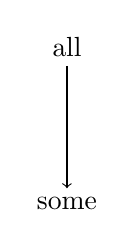
\begin{tikzpicture}
			\node[] at(0, 0) (A) {all};
			\node[] at(0, -2) (B) {some};
			\draw[->] (A) -- (B);
		\end{tikzpicture}
		\caption{Hasse diagram for $\lbrace \textit{all}, \textit{some}\rbrace$}\label{fig2:hasse-scalar} 
	\end{subfigure}	
	\hfill
	\begin{subfigure}[t]{.45\linewidth}
		\centering
		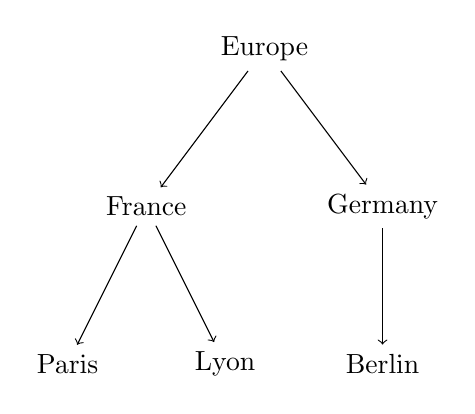
\begin{tikzpicture}
			\node[] at(1.5, 2) (E) {Europe};
			\node[] at(0, 0) (F) {France};
			\node[] at(3, 0) (G) {Germany};
			\node[] at(-1, -2) (P) {Paris};
			\node[] at(1, -2) (L) {Lyon};
			\node[] at(3, -2) (B) {Berlin};
			\draw[->] (F) -- (P);
			\draw[->] (F) -- (L);
			\draw[->] (G) -- (B);
			\draw[->] (E) -- (F);
			\draw[->] (E) -- (G);
		\end{tikzpicture}
		\caption{Hasse diagram for $\lbrace \textit{Europe}, \textit{France}, \textit{Germany}, \textit{Paris}, \textit{Lyon}, \textit{Berlin} \rbrace$}\label{fig2:hasse-locations}
	\end{subfigure}
	\caption{Hasse diagrams generated by $\vDash$ on two possible sets of propositional alternatives.}\label{fig2:hasse}
\end{figure}

How are these diagrams obtained from propositional alternatives, and the entailment relations between them? Formally, a Hasse diagram is a directed graph, as defined in (\ref{ex2:directed-graph}). The only difference between a graph and a directed graph, is that the edges of a directed graph have a direction, i.e. they correspond to ordered pairs instead of sets of cardinality 2. If $[N_1, N_2]$ is a directed edge, $[N_1, N_2]$ is visually represented as $N_1 \rightarrow N_2$. Paths are also directed, and so is the ancestor relation (see (\ref{ex2:directed-graph-path}) and (\ref{ex2:directed-ancestor})). Directed graphs are designed to model \textit{asymmetric} relations, like $\vDash$.

\begin{exe}
	\ex {\textsc{\textbf{Directed graph}}. A directed graph is defined by a set of nodes $\mathcal{N}$ and by a set of directed edges $\mathcal{E}$ between elements of $\mathcal{N}$. Directed edges are defined as ordered pairs of nodes: $\mathcal{E} \subseteq \lbrace [N_1, N_2] \ | \ (N_1, N_2) \in \mathcal{N}^2\rbrace$}\label{ex2:directed-graph}
	\ex {\textit{Directed Path.} Let $G = (\mathcal{N}, \mathcal{E})$ be a directed graph. Let $(N_1, N_2) \in \mathcal{N}^2$ be two nodes of $G$. There is a path in $G$ between $N_1$ and $N_2$ (abbreviated $N_1 \stackrel{G}{\leadsto}  N_2$) iff $N_1$ can be connected to $N_2$ by a series of directed edges in $G$, i.e. $\exists (e_1, ... e_k) \in \mathcal{E}^k. \ e_1^{(0)} = N_1 \wedge e_k^{(1)} = N_2  \wedge \forall i \in [1; k-1]. \ e_i^{(1)} = e_{i+1}^{(0)}$, where, for any edge $e$,  $e = [e^{(0)}, e^{(1)}]$.}\label{ex2:directed-graph-path}
	\ex {\textsc{\textbf{Ancestor relation}} (directed version). Let $G = (\mathcal{N}, \mathcal{E})$ be a directed graph. Let $(N_1, N_2) \in \mathcal{N}^2$. $N_1$ is an ancestor of $N_2$ iff $N_1 \stackrel{G}{\leadsto} N_2$.}\label{ex2:directed-ancestor}
\end{exe}

The directed graphs (not yet the Hasse diagrams) induced by $\vDash$ on the sets of alternatives from Figure \ref{fig2:hasse}, are given in Figure \ref{ex2:graph-entailment}. In these graphs, there is a directed edge $[p, q]$ between two nodes corresponding to propositions $p$ and $q$, iff $q \vDash p$. Figure \ref{fig2:entailment-graph-scalar} already looks like the corresponding Hasse diagram in Figure \ref{fig2:hasse-scalar}, but Figure  \ref{fig2:entailment-graph-locations} does not: it features a few more directed edges (in red) than its Hasse counterpart in Figure \ref{fig2:hasse-locations}.

\begin{figure}[H]
	\centering
	\begin{subfigure}[t]{.45\linewidth}
		\centering
		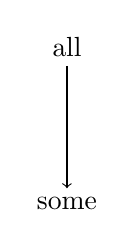
\begin{tikzpicture}
			\node[] at(0, 0) (A) {all};
			\node[] at(0, -2) (B) {some};
			\draw[->] (A) -- (B);
		\end{tikzpicture}
		\caption{Directed graph induced by $\vDash$ on $\lbrace \textit{all}, \textit{some} \rbrace$}\label{fig2:entailment-graph-scalar}
	\end{subfigure}	
	\hfill
	\begin{subfigure}[t]{.45\linewidth}
		\centering
		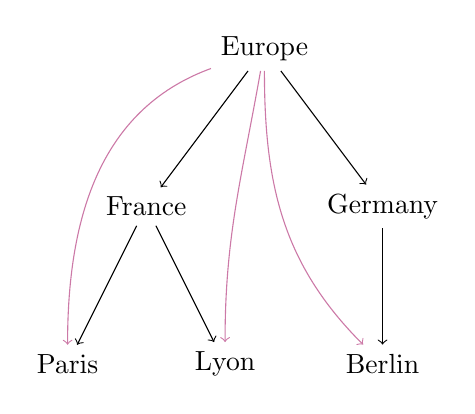
\begin{tikzpicture}
			\node[] at(1.5, 2) (E) {Europe};
			\node[] at(0, 0) (F) {France};
			\node[] at(3, 0) (G) {Germany};
			\node[] at(-1, -2) (P) {Paris};
			\node[] at(1, -2) (L) {Lyon};
			\node[] at(3, -2) (B) {Berlin};
			\draw[->] (F) -- (P);
			\draw[->] (F) -- (L);
			\draw[->] (G) -- (B);
			\draw[->] (E) -- (F);
			\draw[->] (E) -- (G);
			\draw[->,color=red] (E) to [out=-90,in=135] (B);
			\draw[->,color=red] (E) to [out=-100,in=90] (L);
			\draw[->,color=red] (E) to [out=-160,in=90] (P);
		\end{tikzpicture}
		\caption{Directed graph induced by $\vDash$ on $\lbrace \textit{Europe}, \textit{France}, \textit{Germany}, \textit{Paris}, \textit{Lyon}, \textit{Berlin} \rbrace$}\label{fig2:entailment-graph-locations}
	\end{subfigure}
	\caption{Directed graphs generated by $\vDash$ on two possible sets of propositional alternatives.}\label{ex2:graph-entailment}
\end{figure}

How do Hasse diagrams eliminate these few superfluous edges? The Hasse diagrams we are interested in correspond to the transitive reduction of the graphs in Figure \ref{ex2:graph-entailment}, which were induced by $\vDash$ on sets of propositional alternatives. The transitive reduction operation precisely gets rid of the red edges in Figure \ref{fig2:hasse-locations}, based on the idea that such edges correspond to paths formed by the black ones. The formal (though, non constructive) definition of a transitive reduction, is given in (\ref{ex2:transitive-reduction}). This definition maps the graphs in Figure \ref{ex2:graph-entailment}, to the Hasse diagrams in Figure \ref{fig2:hasse}.

\begin{exe}
	\ex {\textsc{\textbf{Transitive reduction of a graph}}. Let $G = (\mathcal{N}, \mathcal{E})$ be a graph. The transitive reduction $G'$ of $G$ is the graph:
	\begin{itemize}
		\item Whose set of nodes is $\mathcal{N}$;
		\item Whose edges are the smallest set $\mathcal{E'}$ s.t. $\forall (N_1, N_2) \in \mathcal{N}. \ N_1 \stackrel{G}{\leadsto} N_2 \iff N_1 \stackrel{G'}{\leadsto} N_2$
		\end{itemize}}\label{ex2:transitive-reduction}
\end{exe}

The Hasse diagram in Figure \ref{fig2:hasse-locations} is basically a rooted tree, and may look like a Qtree, but this is not a generality. For instance, the Hasse diagram in Figure \ref{fig2:hasse-scalar} is not connected, so is not even a tree. Additionally, not all sets of propositional alternatives, even if their Hasse diagram is tree-like, are guaranteed to verify the partition property of Qtrees. The next Section focuses on how Hasse diagrams can be used to determine how alternatives relate to each other in terms of granularity. This will eventually allow us to encode granularity in the structure of Qtree.



\subsection{Alternatives and granularity}

In this Section, we use a notion of granularity to constrain what kind of Qtree can be evoked by a simplex assertive LFs. We consider simplex LFs to be LFs which do not contain a node of type \texttt{t} besides their root.\footnote{Nina Haslinger suggested that this condition \textit{may} be relaxed under certain contexts. For instance, a disjunctive LF denoting $p$, may sometimes be understood as simplex, and generate Qtrees based on the recipe presented later in this Chapter. The exact circumstances under which this is possible, should be fleshed out, but will not be the focus of this dissertation. One intuition, suggested by Nina, is that an overt QuD may indicate what is relevant, and in turn determine what should be considered ``simplex'' when computing implicit Qtrees (and comparing such Qtrees to the overt QuD). Another intuition, is that the ``simplex'' character of an LF, may be partly driven by focus.} The goal is to organize the layers of a Qtree in terms of how specific the nodes in this layer are. Why is an external notion of granularity needed to structure Qtree? In the Qtree sketched in e.g. Figure \ref{fig2:paris-qtree}, each layer corresponds to an intuitive degree of specificity: a by-country layer dominates a by-city layer. Though intuitive, this kind of configuration is not the only one to verify the Qtree property. The tree in Figure \ref{fig2:paris-qtree-mixed}, where the \textit{Germany}-node is replaced by its children, is also a Qtree: at our level of approximation, all countries but Germany, plus all the German cities, partition the set of all possible locations, and, each country represented in this tree is properly partitioned by the set of its cities.


\begin{figure}[H]
	\centering
		\begin{forest}
			[{CS\\
				Jo grew up in...}[\textcolor{blue}{France}[\textcolor{orange}{{\fbox{Paris}}}][\textcolor{orange}{Lyon}][\textcolor{orange}{...}]][\textcolor{orange}{Berlin}][\textcolor{orange}{...}][\textcolor{blue}{Italy}[\textcolor{orange}{...}]][\textcolor{blue}{...}]]
		\end{forest}
		\caption{``Unintuitive'' Qtree for (\ref{ex2:city-partition}) = \textit{Which city did Jo grow up in?}, where layers exhibit ``mixed granularity''.}\label{fig2:paris-qtree-mixed}
	\end{figure}

To derive Qtrees like Figure \ref{fig2:paris-qtree}, and rule-out Qtrees like Figure \ref{fig2:paris-qtree-mixed}, we need a notion of granularity that can transfer into the Qtree layers. We now show that a relation of same-granularity can be derived from Hasse diagrams induced by $\vDash$ on ``complete'' sets of propositional alternatives. Considering such diagrams, where \textit{all} relevant alternatives are considered, we take that two nodes (two propositional alternatives) have same granularity if they are equidistant (in terms of path length) to any common ancestor and common descendant they may have. We also take that any node has the same granularity as itself. This relation, defined in (\ref{ex2:granularity}) is close in spirit to \textcite{Ippolito2019}'s \textit{Specificity Condition}.\footnote{However, the structure on which this condition operates in \citeauthor{Ippolito2019}'s model, appears slightly different (\textit{Structured Sets of Alternatives}). Also, the \textit{Specificity Condition} is not taken to be a relation, but a rather, a constraint defining which kind of alternatives can be contrasted in e.g. disjunctive environments.} Note that this definition constitutes a universal statement, so nodes that do \textit{not} have any common ancestor or descendant, automatically have same-granularity.\footnote{This will be discussed in more detail when dealing with scalar alternatives such as $\langle$\textit{some}, \textit{all}$\rangle$, in Chapter \ref{chap:scalarity}. It will be crucial that such alternatives, which do \textit{not} have a common ancestor in their Hasse diagram (see Figure \ref{fig2:hasse-scalar}), \textit{can} be seen as same-granularity.}

\begin{exe}
	\ex {\textsc{\textbf{Same granularity relation}} ($\sim_g$). Let $p$ and $q$ be two propositions belonging to the same set of propositional alternatives. If $p=q$, then $p \sim_g q$. If not, let $H$ be the Hasse diagram induced by $\vDash$ on the set of propositional alternatives to $p$ and $q$. If for all common ancestor $r$ of both $p$ and $q$ in $H$ and for all common descendant $r'$ of both $p$ and $q$ in $H$, the paths from $r$ to $p$ and $r$ to $q$ have same length, and the paths from $p$ to $r'$ and $q$ to $r'$ have same length, then $p \sim_g q$.}\label{ex2:granularity}
\end{exe}


Figure \ref{fig2:hasse-gran} show a few simple configurations for which $p$ and $q$ do or do not have same granularity.
\begin{figure}[H]
	\centering
	\begin{subfigure}[b]{.15\linewidth}
		\centering
		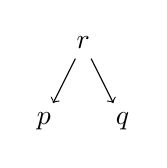
\begin{tikzpicture}
			\node[] (A) at (0,0) {$r$};
			\node[] (B) at (-.5, -1) {$p$};
			\node[] (C) at (.5, -1) {$q$};
			
			\path [->] (A) edge node[left] {} (B);
			\path [->] (A) edge node[left] {} (C);
		\end{tikzpicture}
		\caption{$p\sim_g q$}
	\end{subfigure}
	\hfill
	\begin{subfigure}[b]{.15\linewidth}
		\centering
		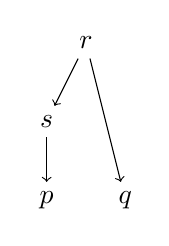
\begin{tikzpicture}
			\node[] (A) at (0, 0) {$r$};
			\node[] (B) at (-.5, -2) {$p$};
			\node[] (C) at (.5, -2) {$q$};
			\node[] (D) at (-.5, -1) {$s$};
			
			\path [->] (A) edge node[left] {} (D);
			\path [->] (A) edge node[left] {} (C);
			\path [->] (D) edge node[left] {} (B);
		\end{tikzpicture}
		\caption{$p\not\sim_g q$}
	\end{subfigure}
	\hfill
	\begin{subfigure}[b]{.15\linewidth}
		\centering
		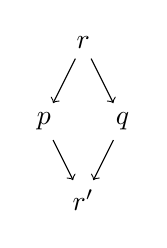
\begin{tikzpicture}
			\node[] (A) at (0,0) {$r$};
			\node[] (B) at (-.5, -1) {$p$};
			\node[] (C) at (.5, -1) {$q$};
			\node[] (D) at (0, -2) {$r'$};
			
			\path [->] (A) edge node[left] {} (B);
			\path [->] (A) edge node[left] {} (C);
			\path [->] (B) edge node[left] {} (D);
			\path [->] (C) edge node[left] {} (D);
		\end{tikzpicture}
		\caption{$p\sim_g q$}
	\end{subfigure}\hfill
	\begin{subfigure}[b]{.15\linewidth}
		\centering
		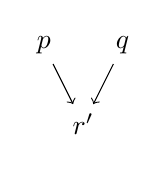
\begin{tikzpicture}
			\node[] (B) at (-.5, -1) {$p$};
			\node[] (C) at (.5, -1) {$q$};
			\node[] (D) at (0, -2) {$r'$};
			
			\path [->] (B) edge node[left] {} (D);
			\path [->] (C) edge node[left] {} (D);
		\end{tikzpicture}
		\caption{$p\sim_g q$}
	\end{subfigure}
	\hfill
	\begin{subfigure}[b]{.15\linewidth}
		\centering
		\begin{tikzpicture}
			\node[] (B) at (-.5, -1) {$p$};
			\node[] (C) at (.5, -1) {$q$};
			
		\end{tikzpicture}
		\caption{$p\sim_g q$}
	\end{subfigure}
	\caption{Different Hasse diagrams for $\vDash$ influence whether $p$ and $q$ are same-granularity.}\label{fig2:hasse-gran}
\end{figure}



We now leverage this relation between propositions to define the layers of a Qtree as partitions induced by sets of same-granularity alternatives. We first observe that the relation $\sim_g$ defined in (\ref{ex2:granularity}) can be used to divide the set of propositional alternatives to a given LF, into subsets sharing the same level of granularity. This gives rise to a ``tiered'' set of alternatives, as defined in (\ref{ex2:tiered-alternatives}). 
\begin{exe}
	\ex {\textsc{\textbf{Tiered set of propositional alternatives}}. Let $X$ be a sentence denoting a proposition $p$. A tiered set of propositional alternatives to $X$, is the set of sets of propositions, whose elements are the maximal sets of propositions related by the same-granularity relation. In other words,  $\mathcal{A}_{p, X}^{\sim_g} = \lbrace \lbrace r \in \mathcal{A}_{p, X} \ | \ r \sim_g q \rbrace \ | \ q \in \mathcal{A}_{p, X}\rbrace$. If $\sim_g$ is an equivalence relation, $\mathcal{A}_{p, X}^{\sim_g}$ is a partition.} \label{ex2:tiered-alternatives}
\end{exe}

Tiered sets of alternatives are quite close to the \textit{Structured Sets of Alternatives} defined in \textcite{Ippolito2019}. One difference however, is that tiered sets of propositional alternatives are \textit{not} assumed to include propositions corresponding to alternatives that are more complex than the original LF. The elements of a tiered set of propositional alternatives are sets of propositions and form same-granularity ``tiers'', as defined in (\ref{ex2:granularity-tier}). These tiers will be used to form Qtree layers. If $\sim_g$ is an equivalence relation when restricted to a specific set of propositional alternatives, then the resulting tiered set of alternatives will partition it, i.e. same-granularity tiers will be cells.

\begin{exe}
	\ex {\textsc{\textbf{Same-granularity tier}}. Let $X$ be a sentence denoting a proposition $p$, and $\mathcal{A}_{p, X}$ its set of propositional alternatives. Let $q \in \mathcal{A}_{p, X}$. The set of same-granularity alternatives to $q$ (in $\mathcal{A}_{p, X}$), is the set of propositions in $\mathcal{A}_{p, X}$ sharing same-granularity with $q$. We call this set $\mathcal{A}^q_{p, X}$. $\mathcal{A}^q_{p, X} = \lbrace r \in \mathcal{A}_{p, X} \ | \ r \sim_g q\rbrace$. $\mathcal{A}^q_{p, X}$ is a subset of the tiered set of propositional alternatives to $X$, $\mathcal{A}_{p, X}^{\sim_g}$. Moreover, if $\sim_g$ is an equivalence relation, then $\mathcal{A}^q_{p, X}$ constitutes a cells of $\mathcal{A}_{p, X}^{\sim_g}$. }\label{ex2:granularity-tier}
\end{exe}

\subsection{Leveraging alternatives to generate Qtrees}
We are now equipped to devise a recipe generating Qtrees out of simplex sentences, based on tiered sets of propositional alternatives. We start by considering the standard constraint on question-answer pairs, given in (\ref{ex2:con-q-a}). This constraint establishes a connection between the standard set of alternatives derived from a sentence involving focus, and the kind of question this sentence answers.

\begin{exe}
	\ex {\textsc{\textbf{Constraint on question-answer pairs}} (\citenp{Rooth1992}, to be revised). A good question-answer pair $(Q, A)$ is s.t. $\llbracket Q \rrbracket \subseteq \llbracket A\rrbracket^f$, where:
	\begin{itemize}
		\item $\llbracket Q \rrbracket$ corresponds to the alternative semantics of the question;
		\item $\llbracket A\rrbracket^f$ corresponds to the focus semantic value of the answer, i.e. the set of propositions denoted by LFs obtained from $A$ \textit{via} the substitution of $A$'s focused material by a same-type element.
		\end{itemize}}\label{ex2:con-q-a}
\end{exe}

Let us show that this constraint is not sufficient (though, a good starter) for a model of questions evoked by assertions. We assume that $A$ corresponds to the sentence \textit{Jo grew up in PARIS}, where \textit{PARIS} is focused. The focus semantic value of $A$ then involves propositions denoted by LFs of the form \textit{Jo grew up in l}, with \textit{l} a location, e.g. \textit{Paris}, \textit{France}, or \textit{Germany}. If the only constraint on the question $Q$ accommodated from $A$ was that $\llbracket Q \rrbracket$ should be a subset of  $\llbracket A\rrbracket^f$, then, in principle, $\llbracket Q \rrbracket$ could be made of the three propositions that \textit{Jo grew up in Paris}, \textit{Jo grew up in France}, and \textit{Jo grew up in Germany}. Granted that Paris is in France, and that France and Germany are disjoint, this set of alternatives would induce a partition of the CS of the form $\lbrace \neg \textit{France} \wedge \neg \textit{Germany}, \textit{Germany}, \textit{France} \wedge \neg \textit{Paris}, \textit{Paris}\rbrace$. This appears similar to the mixed-granularity layer that we said was problematic in Figure \ref{fig2:paris-qtree-mixed}. So not all questions allowed by (\ref{ex2:con-q-a}), given a fixed assertion, appear to make sense. There are two ways to alter (\ref{ex2:con-q-a}) to avoid that kind of configuration: modify the relation between $\llbracket Q\rrbracket$ and $\llbracket A \rrbracket^f$, and/or, change $\llbracket A \rrbracket^f$ into something else.

We in fact opt for both options, and reuse the ideas presented in the previous Section. Specifically, we consider two subcases: the case in which $\llbracket Q \rrbracket$ simply corresponds to $\lbrace \llbracket A \rrbracket \rbrace$, and induces a partition of the CS of the form $\lbrace \llbracket A \rrbracket, \neg\llbracket A \rrbracket \rbrace$; and the case foreshadowed in the previous Section, in which $\llbracket Q \rrbracket$ corresponds to same-granularity alternatives to $\llbracket A \rrbracket$. These two cases are repeated in (\ref{ex2:con-q-a-gran}).

\begin{exe}
	\ex {\textsc{\textbf{Constraint on question-answer pairs}} (first revision). Let $X$ be a LF denoting $p$. $X$ evokes a question that is either:
		\begin{enumerate}[(i)]
			\item\label{ex2:con-q-a-gran-singleton} $\llbracket Q \rrbracket = \lbrace p \rbrace$;
			\item\label{ex2:con-q-a-gran-tier} $\llbracket Q \rrbracket = \mathcal{A}^p_{p, X}$, the set of same-granularity alternatives to $p$.
	\end{enumerate}}\label{ex2:con-q-a-gran}
\end{exe}


(\ref{ex2:con-q-a-gran}) allows assertions to evoke multiple potential Qtrees. According to (\ref{ex2:con-q-a-gran}), an assertion such as \textit{Jo grew up in Paris}, will either evoke the question $\llbracket Q \rrbracket = \lbrace \textit{Paris} \rbrace$, inducing a partition of the CS of the form $\lbrace \textit{Paris}, \neg\textit{Paris}\rbrace$, and corresponding to the polar question of whether or not Jo grew up in Paris; or, $\llbracket Q \rrbracket = \lbrace \textit{Paris}, \textit{Lyon}, \textit{Nice}, ..., \textit{Berlin}, ..., \textit{Rome}, ... \rbrace$, inducing a similar partition of the CS, and corresponding to the \textit{wh}-question \textit{In which city did Jo grow up?}. These partitions are represented in Figure \ref{fig2:one-layer-qtrees}. 

\begin{figure}[H]
	\centering
	\begin{subfigure}[t]{.45\linewidth}
		\centering
		\begin{forest}
			[CS [\textcolor{orange}{Paris}] [\textcolor{orange}{$\neg${Paris}}]]
		\end{forest}
		\caption{A Qtree for (\ref{ex2:city-assertion}) assuming (\ref{ex2:con-q-a-gran}\ref{ex2:con-q-a-gran-singleton}) }\label{fig2:one-layer-polar}
	\end{subfigure}
	\hfill
	\begin{subfigure}[t]{.5\linewidth}
		\centering
		\begin{forest}
			[CS [\textcolor{orange}{Paris}] [\textcolor{orange}{Lyon}] [\textcolor{orange}{...}] [\textcolor{orange}{Berlin}] [\textcolor{orange}{...}] [\textcolor{orange}{Rome}]]
		\end{forest}
		\caption{A Qtree for (\ref{ex2:city-assertion}) assuming (\ref{ex2:con-q-a-gran}\ref{ex2:con-q-a-gran-tier})}\label{fig2:one-layer-wh}
	\end{subfigure}
	\caption{One-layer Qtrees generable from (\ref{ex2:con-q-a-gran}) and the sentence (\ref{ex2:city-assertion})=\textit{Jo grew up in Paris}.}\label{fig2:one-layer-qtrees}
\end{figure}

The above partitions seem more in line with intuitions than the pathological ones generable from (\ref{ex2:con-q-a}). However, they still do not form layered Qtrees. Therefore, (\ref{ex2:con-q-a-gran}) is still not powerful enough to capture the specificity differences sketched in Figure \ref{fig2:qtrees-diff-gran} among others. Going one step further, we can assume that the Qtrees compatible with a sentence, are either generated by the proposition $p$ denoted by the sentence (thus creating a Qtree like Figure \ref{fig2:one-layer-polar}), or, by the sentence's tiered set of propositional alternatives, as defined in (\ref{ex2:tiered-alternatives}). Specifically in the latter case, it will be assumed that each layer of the Qtree corresponds to the partition induced on the CS by a same-granularity tier of propositional alternatives, and that layers are ordered in terms of granularity. Figure \ref{fig2:one-layer-wh} constitutes the simplest subcase of this principle, in which only one layer gets generated out of same-granularity alternatives to $p$. In any case, verifying nodes are defined as the leaves of the tree entailing $p$ (i.e. contained in $p$). This is formalized in (\ref{ex2:qtree-simplex-def}). In this definition, (\ref{ex2:qtree-simplex-def}\ref{pt2:simplex-qtree-wh}) may be seen as a subcase of (\ref{ex2:qtree-simplex-def}\ref{pt2:simplex-qtree-tiered}), in which the $p$-chain set to $p$ only.

\begin{exe}
	\ex {\textsc{\textbf{Qtrees for simplex LFs}}.
		Let $X$ be a simplex LF denoting $p$, not settled in the CS. Let $\mathcal{A}_{p, X}$ be the set $X$'s propositional alternatives. For any $q \in  \mathcal{A}_{p, X}$, let $\mathcal{A}^q_{p, X} \subseteq \mathcal{A}_{p, X}$ be the set of alternatives from $\mathcal{A}_{p, X}$ sharing same granularity with $q$. We assume for simplicity that for any $q$, $\mathcal{A}^q_{p, X}$ partitions the CS. A Qtree for $X$ is either:
		\begin{enumerate}[(i)]
			\item\label{pt2:simplex-qtree-polar} A depth-1 Qtree whose leaves denote $\mathfrak{P}_{\lbrace p \rbrace, CS} = \lbrace p, \neg p\rbrace$
			\item\label{pt2:simplex-qtree-wh} A depth-1 Qtree whose leaves denote $\mathfrak{P}_{\mathcal{A}^p_{p, X}, CS} = \mathcal{A}^p_{p,X}$.
			\item\label{pt2:simplex-qtree-tiered} A depth-$k$ Qtree ($k > 1$) constructed in the following way:
			\begin{itemize}
				\item Formation of a ``$p$-chain'' $p_0 = p \subset p_1 \subset ... \subset p_n$ where $p_0, ...,  p_n$ are all in $\mathcal{A}_{p, X}$ but belong to different granularity tiers in $\mathcal{A}_{p, X}^{\sim_g}$:  $\mathcal{A}^{p_0}_{p, X}$ $\neq$ $\mathcal{A}^{p_1}_{p, X}$ $\neq$ ... $\neq$$\mathcal{A}^{p_n}_{p, X}$.
				\item Generation of the ``layers'' of the Qtree, based on the partitions induced by the granularity tiers corresponding to each element of the $p$-chain:\\ \begin{small}$\left\lbrace\mathfrak{P}_{\mathcal{A}^{p_i}_{p, X}, CS} \ | \ i \in [0;n]\right\rbrace$\end{small}.
				\item Determination of the edges between nodes (cells) of adjacent layers (and between the highest layer and the root), based on the subset relation.\footnote{This may not always create well-formed Qtrees. Chapter \ref{chap:scalarity} will explore such cases update (\ref{ex2:qtree-simplex-def}) in consequence.}
			\end{itemize}
		\end{enumerate}
		In any case,  \setlength{\fboxsep}{1pt}\fbox{verifying nodes} are defined as the set of leaves entailing $p$.
	}\label{ex2:qtree-simplex-def}
\end{exe}


\subsection{Applying the recipe to two simple sentences}

We can now apply (\ref{ex2:qtree-simplex-def}) to sentences like (\ref{ex2:city-assertion}) and (\ref{ex2:country-assertion}), repeated below.

\begin{exe}
	\exr{ex2:city-country-assertions}
	\begin{xlist}
		\ex {Jo grew up in Paris.}
		\ex {Jo grew up in France.}
	\end{xlist}
\end{exe}

We start with (\ref{ex2:city-assertion}), and assume that its alternatives are of the form \textit{Jo grew up in l}, with \textit{l} a city or a country. Taking for granted that ``city'' propositions and ``country'' propositions form two distinct granularity tiers, the tiered set of propositional alternatives to (\ref{ex2:city-assertion}), will be as in (\ref{ex2:city-tiered-alt}).

\begin{exe}
	\ex {$\mathcal{A}_{\textit{Paris}, (\ref{ex2:city-assertion})}^{\sim_g} = \lbrace \lbrace \textit{Paris}, \textit{Lyon}, ..., \textit{Berlin}, ...\rbrace, \lbrace\textit{France}, \textit{Germany}, ...\rbrace\rbrace$\\
	\phantom{$\mathcal{A}_{\textit{Paris}, (\ref{ex2:city-assertion})}^{\sim_g}$} $=\lbrace\lbrace p \ | \ \exists l. \ \text{$l$ is a city} \wedge \ p = \lambda w. \ \text{Jo grew up in $l$ in $w$}\rbrace,$\\
	\phantom{$\mathcal{A}_{\textit{Paris}, (\ref{ex2:city-assertion})}^{\sim_g} = \lbrace$}$\lbrace p \ | \ \exists l. \ \text{$l$ is a country} \wedge \ p = \lambda w. \ \text{Jo grew up in $l$ in $w$}\rbrace\rbrace$}\label{ex2:city-tiered-alt}
\end{exe} 



First, we can generate a Qtree for (\ref{ex2:city-assertion})  using principle (\ref{ex2:qtree-simplex-def}\ref{pt2:simplex-qtree-polar}). This Qtree will have the CS as root, and two leaves corresponding to the propositions that \textit{Jo grew up in Paris}, and \textit{Jo did not grow up in Paris} (assuming this matter is not settled in the CS). This Qtree is depicted in Figure \ref{fig2:city-qtree-polar}. Intuitively, it corresponds to the question of whether or not Jo grew up in Paris.

Second, we can use principle (\ref{ex2:qtree-simplex-def}\ref{pt2:simplex-qtree-wh}). To do so, we must determine the set of same-granularity alternatives to the prejacent proposition that \textit{Jo grew up in Paris}. This set, labeled $\mathcal{A}_{\textit{Paris}, (\ref{ex2:city-assertion})}^{\textit{Paris}}$, corresponds to the first element of the tiered set of propositional alternatives $\mathcal{A}_{\textit{Paris}, (\ref{ex2:city-assertion})}^{\sim_g}$ in  (\ref{ex2:city-tiered-alt}). It is repeated in (\ref{ex2:city-gran-alt}). The alternatives contained in $\mathcal{A}_{\textit{Paris}, (\ref{ex2:city-assertion})}^{\textit{Paris}}$ are all exclusive (cities are spatially disjoint), and moreover cover the space of possibilities. So, once intersected with the CS, they already form a partition of the CS. According to principle (\ref{ex2:qtree-simplex-def}\ref{pt2:simplex-qtree-wh}), this partition correspond to the leaves of the resulting Qtree. This Qtree is depicted in Figure \ref{fig2:city-qtree-wh}. Intuitively, it corresponds to the question of which city Jo grew up in.


\begin{exe}
	\ex {$\mathcal{A}_{\textit{Paris}, (\ref{ex2:city-assertion})}^{\textit{Paris}} = \lbrace \textit{Paris}, \textit{Lyon}, ..., \textit{Berlin}, ...\rbrace$\\
		\phantom{$\mathcal{A}_{\textit{Paris}, (\ref{ex2:city-assertion})}^{\sim_g}$} $=\lbrace p \ | \ \exists l. \ \text{$l$ is a city} \wedge \ p = \lambda w. \ \text{Jo grew up in $l$ in $w$}\rbrace$\\
		\phantom{$\mathcal{A}_{\textit{Paris}, (\ref{ex2:city-assertion})}^{\sim_g}$} $=\mathfrak{P}_{\lbrace \textit{Paris}, \textit{Lyon}, ..., \textit{Berlin}, ...\rbrace, CS}$}\label{ex2:city-gran-alt}
\end{exe} 

Third and lastly, we can use principle (\ref{ex2:qtree-simplex-def}\ref{pt2:simplex-qtree-tiered}), which constitutes are multi-layer generalization of principle (\ref{ex2:qtree-simplex-def}\ref{pt2:simplex-qtree-wh}). To do so, we need to define a $p$-chain of propositions entailed $p$ = $\lambda w. \ $\textit{Jo grew up in Paris in $w$}. The tiered set of alternatives posited in (\ref{ex2:city-tiered-alt}) contains one such proposition, namely $p' = \lambda w. \ $\textit{Jo grew up in France in $w$}. The resulting Qtree will therefore be made of three layers: the CS (root), the partition generated by the same granularity alternatives to $p'$, and the partition generated by the same granularity alternatives to $p$, already defined in (\ref{ex2:city-gran-alt}). The set of same-granularity alternatives to $p'$, labeled $\mathcal{A}_{\textit{Paris}, (\ref{ex2:city-assertion})}^{\textit{France}}$, corresponds to the second element of the tiered set of propositional alternatives $\mathcal{A}_{\textit{Paris}, (\ref{ex2:city-assertion})}^{\sim_g}$ in  (\ref{ex2:city-tiered-alt}). It is repeated in (\ref{ex2:country-gran-alt}). The alternatives contained in $\mathcal{A}_{\textit{Paris}, (\ref{ex2:city-assertion})}^{\textit{France}}$ are all exclusive (country are spatially disjoint), and moreover cover the space of possibilities. So, once intersected with the CS, they already form a partition of the CS. 

\begin{exe}
	\ex {$\mathcal{A}_{\textit{Paris}, (\ref{ex2:city-assertion})}^{\textit{France}} = \lbrace \textit{France}, \textit{Germany}, ...\rbrace$\\
		\phantom{$\mathcal{A}_{\textit{Paris}, (\ref{ex2:city-assertion})}^{\sim_g}$} $=\lbrace p \ | \ \exists l. \ \text{$l$ is a country} \wedge \ p = \lambda w. \ \text{Jo grew up in $l$ in $w$}\rbrace$\\
		\phantom{$\mathcal{A}_{\textit{Paris}, (\ref{ex2:city-assertion})}^{\sim_g}$} $=\mathfrak{P}_{\lbrace \textit{France}, \textit{Germany}, ...\rbrace, CS}$}\label{ex2:country-gran-alt}
\end{exe} 

As per principle (\ref{ex2:qtree-simplex-def}\ref{pt2:simplex-qtree-tiered}), a Qtree evoked by (\ref{ex2:city-assertion}) will then have the CS as top layer, the nodes corresponding to the partition in (\ref{ex2:country-gran-alt}) as middle layer, and the nodes corresponding to the partition in (\ref{ex2:city-gran-alt}) as bottom (leaf) layer. Connectivity between layers is straightforward: it corresponds to the inclusion relation between cities and countries, and between countries and ``the whole world'' ($\sim$CS). The resulting Qtree is given in Figure \ref{fig2:city-qtree-tiered}. Intuitively, it corresponds to the question of which city Jo grew up in, but such that this question is decomposed into two subquestions: first, which country Jo grew up in; then, knowing the country, which city Jo grew up in, in that country.


\begin{figure}[H]
	\centering
	\begin{subfigure}[t]{.23\linewidth}
		\centering
		\scalebox{.85}{
		\begin{forest}
			[CS [\textcolor{orange}{\fbox{Paris}}] [\textcolor{orange}{$\neg$Paris}]]
		\end{forest}}
		\caption{Following principle (\ref{ex2:qtree-simplex-def}\ref{pt2:simplex-qtree-polar}).}\label{fig2:city-qtree-polar}
	\end{subfigure}
	\hfill
	\begin{subfigure}[t]{.33\linewidth}
		\centering		\scalebox{.85}{
		\begin{forest}
			[CS [\textcolor{orange}{\fbox{Paris}}] [\textcolor{orange}{Lyon}] [\textcolor{orange}{...}][\textcolor{orange}{Berlin}][\textcolor{orange}{...}]]
		\end{forest}}
		\caption{Following principle (\ref{ex2:qtree-simplex-def}\ref{pt2:simplex-qtree-wh}).}\label{fig2:city-qtree-wh}
	\end{subfigure}
	\hfill
	\begin{subfigure}[t]{.38\linewidth}
		\centering\scalebox{.85}{
		\begin{forest}
			[CS [\textcolor{blue}{France}[\textcolor{orange}{\fbox{Paris}}] [\textcolor{orange}{Lyon}] [\textcolor{orange}{...}]] [\textcolor{blue}{Germany}[\textcolor{orange}{Berlin}][\textcolor{orange}{...}]][\textcolor{blue}{...}]]
		\end{forest}}
		\caption{Following principle (\ref{ex2:qtree-simplex-def}\ref{pt2:simplex-qtree-tiered}).}\label{fig2:city-qtree-tiered}
	\end{subfigure}
	\caption{Possible Qtrees evoked by the assertion (\ref{ex2:city-assertion})=\textit{Jo grew up in Paris}.}\label{fig2:city-qtrees}
\end{figure}

Of course, if more alternatives to (\ref{ex2:city-assertion}) had been posited in the first place, principle (\ref{ex2:qtree-simplex-def}\ref{pt2:simplex-qtree-tiered}) would have produced more Qtrees. For instance, if continent alternative had been considered, the tiered set of propositional alternatives to (\ref{ex2:city-assertion}), $\mathcal{A}_{\textit{Paris}, (\ref{ex2:city-assertion})}^{\sim_g}$, would have been as in (\ref{ex2:city-tiered-alt-plus-continent}), and the Qtrees generated by principle (\ref{ex2:qtree-simplex-def}\ref{pt2:simplex-qtree-tiered}), would have been the one in Figure \ref{fig2:city-qtree-tiered}, plus the one in Figure \ref{fig2:city-qtree-tiered-plus-continent}.

\begin{exe}
	\ex {$\mathcal{A}_{\textit{Paris}, (\ref{ex2:city-assertion})}^{\sim_g} = \lbrace \lbrace \textit{Paris}, \textit{Lyon}, ..., \textit{Berlin}, ...\rbrace, \lbrace\textit{France}, \textit{Germany}, ...\rbrace, \lbrace \textit{Europe}, \textit{Asia}, ...\rbrace\rbrace$\\
		\phantom{$\mathcal{A}_{\textit{Paris}, (\ref{ex2:city-assertion})}^{\sim_g}$} $=\lbrace\lbrace p \ | \ \exists l. \ \text{$l$ is a city} \wedge \ p = \lambda w. \ \text{Jo grew up in $l$ in $w$}\rbrace,$\\
		\phantom{$\mathcal{A}_{\textit{Paris}, (\ref{ex2:city-assertion})}^{\sim_g} = \lbrace$}$\lbrace p \ | \ \exists l. \ \text{$l$ is a country} \wedge \ p = \lambda w. \ \text{Jo grew up in $l$ in $w$}\rbrace$\\
		\phantom{$\mathcal{A}_{\textit{Paris}, (\ref{ex2:city-assertion})}^{\sim_g} = \lbrace$}$\lbrace p \ | \ \exists l. \ \text{$l$ is a continent} \wedge \ p = \lambda w. \ \text{Jo grew up in $l$ in $w$}\rbrace\rbrace$}\label{ex2:city-tiered-alt-plus-continent}
\end{exe} 

\begin{figure}[H]
	\centering
	\scalebox{.85}{
		\begin{forest}
			[CS [Europe [\textcolor{blue}{France}[\textcolor{orange}{\fbox{Paris}}] [\textcolor{orange}{Lyon}] [\textcolor{orange}{...}]] [\textcolor{blue}{Germany}[\textcolor{orange}{Berlin}][\textcolor{orange}{...}]][\textcolor{blue}{...}]][Asia [...]][...] ]
	\end{forest}}
	\caption{An extra Qtree for (\ref{ex2:city-assertion}), generated by principle (\ref{ex2:qtree-simplex-def}\ref{pt2:simplex-qtree-tiered}), assuming that (\ref{ex2:city-assertion})'s tiered set of propositional alternatives is as in (\ref{ex2:city-tiered-alt-plus-continent}). .}\label{fig2:city-qtree-tiered-plus-continent}
\end{figure}

For simplicity and ease of comparison, we will stick to a tiered set of alternatives involving city- and country-tiers, as defined in (\ref{ex2:city-tiered-alt}). Similarly, we can derive Qtrees for (\ref{ex2:country-assertion})=\textit{Jo grew up in France}. This assertion will in fact require less work, because it appears coarser-grained than (\ref{ex2:city-assertion}). To ensure that (\ref{ex2:city-assertion}) and (\ref{ex2:country-assertion}) are analyzed at the same level of approximation, we assume that (\ref{ex2:country-assertion})'s alternatives are also of the form \textit{Jo grew up in l}, with \textit{l} a city or a country. The tiered set of propositional alternatives to (\ref{ex2:country-assertion}) is therefore identical to that of (\ref{ex2:city-assertion}), and given in (\ref{ex2:country-tiered-alt}).

\begin{exe}
	\ex {$\mathcal{A}_{\textit{France}, (\ref{ex2:country-assertion})}^{\sim_g} = \lbrace \lbrace \textit{Paris}, \textit{Lyon}, ..., \textit{Berlin}, ...\rbrace, \lbrace\textit{France}, \textit{Germany}, ...\rbrace\rbrace$\\
		\phantom{$\mathcal{A}_{\textit{France}, (\ref{ex2:country-assertion})}^{\sim_g}$} $=\lbrace\lbrace p \ | \ \exists l. \ \text{$l$ is a city} \wedge \ p = \lambda w. \ \text{Jo grew up in $l$ in $w$}\rbrace,$\\
		\phantom{$\mathcal{A}_{\textit{France}, (\ref{ex2:country-assertion})}^{\sim_g} = \lbrace$}$\lbrace p \ | \ \exists l. \ \text{$l$ is a country} \wedge \ p = \lambda w. \ \text{Jo grew up in $l$ in $w$}\rbrace\rbrace$\\
		\phantom{$\mathcal{A}_{\textit{France}, (\ref{ex2:country-assertion})}^{\sim_g}$}= $\mathcal{A}_{\textit{Paris}, (\ref{ex2:city-assertion})}^{\sim_g}$}\label{ex2:country-tiered-alt}
\end{exe} 


First, we can generate a Qtree for (\ref{ex2:country-assertion}) using principle (\ref{ex2:qtree-simplex-def}\ref{pt2:simplex-qtree-polar}). This Qtree will have the CS as root, and two leaves corresponding to the propositions that \textit{Jo grew up in France}, and \textit{Jo did not grow up in France} (assuming this matter is not settled in the CS). This Qtree is depicted in Figure \ref{fig2:country-qtree-polar}. Intuitively, it corresponds to the question of whether or not Jo grew up in France.

Second, we can use principle (\ref{ex2:qtree-simplex-def}\ref{pt2:simplex-qtree-wh}). To do so, we must determine the set of same-granularity alternatives to the prejacent proposition that \textit{Jo grew up in France}. This set, labeled $\mathcal{A}_{\textit{France}, (\ref{ex2:country-assertion})}^{\textit{France}}$, corresponds to the second element of the tiered set of propositional alternatives $\mathcal{A}_{\textit{France}, (\ref{ex2:country-assertion})}^{\sim_g}$. It is repeated in (\ref{ex2:country-gran-alt2}). This set is also equal to the set of same-granularity alternative to \textit{France}, when the prejacent was \textit{Paris} (see (\ref{ex2:country-gran-alt})). Thus, the alternatives in this set, once intersected with the CS, already form a partition of the CS. According to principle (\ref{ex2:qtree-simplex-def}\ref{pt2:simplex-qtree-wh}), this partition correspond to the leaves of the resulting Qtree. This Qtree is depicted in Figure \ref{fig2:country-qtree-wh}. Intuitively, it corresponds to the question of which country Jo grew up in.


\begin{exe}
	\ex {$\mathcal{A}_{\textit{France}, (\ref{ex2:country-assertion})}^{\textit{France}} = \lbrace \textit{France}, \textit{Germany}, ...\rbrace$\\
		\phantom{$\mathcal{A}_{\textit{France}, (\ref{ex2:country-assertion})}^{\textit{France}}$} $=\lbrace p \ | \ \exists l. \ \text{$l$ is a city} \wedge \ p = \lambda w. \ \text{Jo grew up in $l$ in $w$}\rbrace$\\
		\phantom{$\mathcal{A}_{\textit{France}, (\ref{ex2:country-assertion})}^{\textit{France}}$} $=\mathfrak{P}_{\lbrace \textit{France}, \textit{Germany}, ...\rbrace, CS}$\\
		\phantom{$\mathcal{A}_{\textit{France}, (\ref{ex2:country-assertion})}^{\textit{France}}$} $=\mathcal{A}_{\textit{Paris}, (\ref{ex2:city-assertion})}^{\textit{France}}$}\label{ex2:country-gran-alt2}
\end{exe} 

Third and lastly, we could use principle (\ref{ex2:qtree-simplex-def}\ref{pt2:simplex-qtree-tiered}), but this principle would in fact give us nothing more than principle (\ref{ex2:qtree-simplex-def}\ref{pt2:simplex-qtree-wh}), given our assumptions about (\ref{ex2:country-assertion})'s tiered set of propositional alternatives. This is because no proposition in $\mathcal{A}_{\textit{France}, (\ref{ex2:country-assertion})}^{\sim_g}$ is weaker than $p$=\textit{$\lambda w. \ \textit{Jo grew up in France in $w$}$}, and therefore, the only $p$-chain available in the case of (\ref{ex2:country-assertion}), is made of simply $p$. This $p$-chain would generate one single country-layer beyond the CS root, and the resulting Qtree, would simply be the one in Figure \ref{fig2:country-qtree-wh}.\footnote{Of course, if we had considered continent-level alternatives as well, principle (\ref{ex2:qtree-simplex-def}\ref{pt2:simplex-qtree-tiered}) would have generated an extra Qtree for (\ref{ex2:country-assertion}), characterized by a continent-layer on top of a country-layer. But this would have led us to do the same move for (\ref{ex2:city-assertion}), and thus to generate the Qtree in Figure \ref{fig2:city-qtree-tiered-plus-continent} for that sentence.}

\begin{figure}[H]
	\centering
	\begin{subfigure}[t]{.45\linewidth}
		\centering
		\scalebox{.85}{
			\begin{forest}
				[CS [\textcolor{blue}{\fbox{France}}] [\textcolor{blue}{$\neg$France}]]
		\end{forest}}
		\caption{Following principle (\ref{ex2:qtree-simplex-def}\ref{pt2:simplex-qtree-polar}).}\label{fig2:country-qtree-polar}
	\end{subfigure}
	\hfill
	\begin{subfigure}[t]{.45\linewidth}
		\centering		\scalebox{.85}{
			\begin{forest}
				[CS [\textcolor{blue}{\fbox{France}}] [\textcolor{blue}{Germany}][\textcolor{blue}{...}]]
		\end{forest}}
		\caption{Following principle (\ref{ex2:qtree-simplex-def}\ref{pt2:simplex-qtree-wh}).}\label{fig2:country-qtree-wh}
	\end{subfigure}
	\caption{Possible Qtrees evoked by the assertion (\ref{ex2:country-assertion})=\textit{Jo grew up in France}.}
\end{figure}


Before moving on to ``compositional'' Qtrees, let us take stock.

First, the recipe in (\ref{ex2:qtree-simplex-def}) defines way to determine which parse of the CS assertive sentences evoke. We have discussed in Chapter \ref{chap:introduction} that questions typically correspond to partitions of the CS \textit{in the pragmatic domain}. Semantically, questions are taken to be sets of alternatives. In that sense, Qtrees evoked by sentences should be understood as a form of ``inquisitive pragmatics'' rather than ``inquisitive semantics''. Tiered sets of propositional alternatives may be closer to the latter concept.

Second, the recipe in (\ref{ex2:qtree-simplex-def}) typically generates \textit{multiple} Qtrees out of one assertion. Under our current assumptions,  (\ref{ex2:city-assertion}) gives rise to three possible Qtrees, and (\ref{ex2:country-assertion}), to two. So there is some degree of uncertainty about which Qtree any given sentence actually answers. Very roughly, evoked Qtrees can be ``polar'' (principle (\ref{ex2:qtree-simplex-def}\ref{pt2:simplex-qtree-polar})), ``\textit{wh}'' (principle (\ref{ex2:qtree-simplex-def}\ref{pt2:simplex-qtree-wh})), or ``\textit{wh}-articulated'' (principle (\ref{ex2:qtree-simplex-def}\ref{pt2:simplex-qtree-tiered})). This optionality contrasts with frameworks like inquisitive semantics, in which any given sentence is mapped to a single nonempty downward-closed set of propositions. Given this, our recipe generates more Qtrees than intuitively assumed in the previous Sections.  Additionally, this leads us to define the oddness of a sentence as equivalent to the oddness of \textit{all} sentence-Qtree pairs to sentences can generate. This was already defined in (\ref{ex2:oddness-sentence}), repeated below.

\begin{exe}
	\exr{ex2:oddness-sentence} {\textsc{\textbf{Oddness of a sentence}}. A sentence $S$ is odd if any Qtree $T$ it evokes is odd given $S$.}
\end{exe}


Third, we mentioned that (\ref{ex2:city-assertion}) and (\ref{ex2:country-assertion}), beyond the fact that they are obviously in a relation of logical entailment, are such that (\ref{ex2:city-assertion}) feels more ``fine-grained'' than (\ref{ex2:country-assertion}). This is somehow cashed out by the kind of Qtrees these sentences evoke. Specifically, we observe that some Qtrees (\ref{ex2:city-assertion}) evokes (Figure \ref{fig2:city-qtree-tiered}) constitute refinements of some Qtree (\ref{ex2:country-assertion}) evokes (Figure \ref{fig2:country-qtree-wh}), where refinement is defined as in (\ref{ex2:qtree-refinement}), repeated below. This implication does not hold in the opposite direction: no Qtree (\ref{ex2:country-assertion}) evokes, constitutes a refinement of a Qtree (\ref{ex2:city-assertion}) evokes. So (in a very weak sense) finer-grained assertions evoke finer-grained Qtrees. This observation will be crucial in Chapter \ref{chap:hurford-sentences}.

\begin{exe}
	\exr{ex2:qtree-refinement} {\textsc{\textbf{Qtree refinement}}. Let $T$ and $T'$ be Qtrees. $T$ is a refinement of $T'$ (or: $T$ is finer-grained than $T'$), iff $T'$ can be obtained from $T$ by removing a subset $\mathcal{T}$ of $T$'s subtrees, s.t.:
		\begin{itemize}
			\item if $\mathcal{T}$ contains a subtree rooted in $N$, then, for each node $N'$ that is a sibling of $N$ in $T$, the subtree of $T$ rooted in $N'$, is also in $\mathcal{T}$.
	\end{itemize}}
\end{exe}

We now proceed to define Qtree for complex sentences belonging to the $\lbrace \neg, \vee, \rightarrow\rbrace$-fragment of the language. We will do so inductively, using our recipe for simplex sentences (\ref{ex2:qtree-simplex-def}) as base case, along with specific combination rules corresponding to the inquisitive effect of each operator.


\section{Compositional Qtrees: inductive step}

In the previous Section, we have seen how to derive Qtrees from simplex sentences, containing no operator or connective. In this Section, we clarify how complex sentences, that may be equally informative, and may even have same propositional meaning, may end up packaging information differently from one another, in terms of their evoked Qtrees. This difference in information packaging, will allow us to derive different felicity profiles for these sentences. We start with Qtrees evoked by negated LFs, before moving on to Qtrees evoked by disjunctions and conditionals.

\subsection{Questions evoked by negated LFs}\label{sec:neg}
We assume negated LFs evoke questions that are structurally similar to those evoked by their non-negated counterpart. The only difference resides in the set of verifying nodes, which is ``flipped'' by negation. This is formalized in (\ref{ex2:qtree-neg-def}).\footnote{This approach is perhaps a bit naive; uttering $p$ vs. $\neg p$, does not seem to preferentially answer the same kind of question. More specifically, it seems that uttering negative statements in general conveys the idea that the original question was more likely to be a polar question of the form \textit{whether p?} -- as opposed to a \textit{wh} kind of question. We discuss this more in depth in Chapter \ref{chap:scalarity}.}

\begin{exe}
	\ex {\textsc{\textbf{Qtrees for negated LFs}}. Let $T$ be a Qtree evoked by a LF $X$. A Qtree $T_{\neg}$ for $\neg X$ is obtained from $T$ by:
		\begin{itemize}
			\item retaining $T$'s structure; i.e. if $T = (\mathcal{N}, \mathcal{E}, R)$,  then $T_{\neg} = (\mathcal{N}, \mathcal{E}, R)$, too;
			\item defining $T_{\neg}$'s set of verifying nodes $\mathcal{N}^+(T_{\neg})$ as the set of $T_{\neg}$'s nodes $N$ that are not verifying in $T$ ($N \notin \mathcal{N}^+(T)$) but belong to a layer containing at least one verifying node $N'$ in $T$ ($N' \in \mathcal{N}^+(T)$). In other words:\\
			$\mathcal{N}^+(T_\neg)$ = $\lbrace N \ | \ N \notin \mathcal{N}^+(T) \wedge \exists N' \in \mathcal{N}^+(T). \ d(N, T_\neg)=d(N', T_\neg) \rbrace$\\
			With $d(N, T)$ the depth of a node $N$ in a tree $T$ (see (\ref{ex2:tree-depth})).\footnote{Because $T$ and $T_\neg$ have same structure, it does not matter which Qtree among $T$ and $T_\neg$ is passed as argument to the depth function; in that particular case, $\forall N \in \mathcal{N}. \ d(N, T)=d(N, T_\neg)$.}
		\end{itemize} 
	}\label{ex2:qtree-neg-def}
\end{exe}

The recipe in (\ref{ex2:qtree-neg-def}) is exemplified in the abstract Qtrees in Figure \ref{fig2:qtree-x-neg-x}. 

\begin{figure}[H]
	\centering
	\begin{subfigure}[t]{.45\linewidth}
		\centering
		\begin{forest}
			[A[\fbox{B}[\fbox{E}][\fbox{F}]][C][\fbox{D}[G][H[J][K]][I]]]
		\end{forest}
		\caption{An abstract Qtree for $X$}\label{fig2:qtree-x}
	\end{subfigure}
	\hfill
	\begin{subfigure}[t]{.45\linewidth}
		\centering
		\begin{forest}
			[A[{B}[{E}][{F}]][\fbox{C}][{D}[\fbox{G}][\fbox{H}[J][K]][\fbox{I}]]]
		\end{forest}
		\caption{An abstract Qtree for $\neg X$, derived from Figure \ref{fig2:qtree-x}.}\label{fig2:qtree-neg-x}
	\end{subfigure}
	\caption{An abstract Qtree for $X$ and the abstract Qtree for $\neg X$ derived from it, \textit{via} (\ref{ex2:qtree-neg-def}).}\label{fig2:qtree-x-neg-x}
\end{figure}


It may not seem obvious at this point why and how verifying nodes would occur at intermediate levels in a Qtree; after all, all the Qtrees we have seen so far (derived from simplex sentences) had their verifying nodes at the leaf level. But we will see that Qtrees derived from complex sentences (typically, involving disjunctions and conditionals) can in principle feature intermediate verifying nodes, because such nodes are also derived compositionally.
Now, granted that verifying nodes may indeed occur at different levels, the intuition behind the ``flipping'' algorithm in (\ref{ex2:qtree-neg-def}) is the following. If a node $N$ is verifying in a Qtree $T$ corresponding to an LF $X$, and $N$ is located at depth $k$ in $T$, then somehow the $k$-layer of $T$ is ``addressed'' by $X$. We aim for a pair $(\neg X, T_\neg)$ to address the same layers as $(X, T)$, so $T_\neg$'s verifying nodes should have similar a similar depth distribution as $T$'s verifying nodes. But of course, the two sets of nodes need to be distinct, because negation standardly flips truth values -- hence the by-layer flipping.

It is additionally worth mentioning that, if all verifying nodes in the original Qtree $T$ are leaves, (\ref{ex2:qtree-neg-def}) is simplified: $T_\neg$'s set of verifying nodes is simply the set of leaves in $T$/$T_\neg$ that are not verifying in $T$. This is summarized in (\ref{ex2:qtree-neg-def-leaves}).

\begin{exe}
	\ex {\textsc{\textbf{Qtrees for negated LFs}} (leaf-only version, subcase of (\ref{ex2:qtree-neg-def})). Let $T$ be a Qtree evoked by a LF $X$ s.t. $\mathcal{N}^+(T) \subseteq \mathcal{L}(T)$, where $\mathcal{L}(T)$ refers to $T$'s leaves. A Qtree $T_{\neg}$ for $\neg X$ is obtained from $T$ by:
		\begin{itemize}
			\item retaining $T$'s structure;
			\item defining $T_{\neg}$'s set of verifying nodes as the complement set of $\mathcal{N}^+(T)$ within $\mathcal{L}(T)$:
			$\mathcal{N}^+(T_\neg) = \lbrace N \in \mathcal{L}(T)\ | \ N \notin \mathcal{N}^+(T)\rbrace$ 
		\end{itemize} 
	}\label{ex2:qtree-neg-def-leaves}
\end{exe}

Following this simplified recipe, Qtrees for (\ref{ex2:city-neg-assertion}), which correspond to the negation of (\ref{ex2:city-assertion}), are given below. They are obtained from Figure \ref{fig2:city-qtrees}, by simply flipping boxed nodes at the leaf level. These new Qtree capture the intuition that (\ref{ex2:city-neg-assertion}) can answer three kinds of question: a question about whether or not Jo grew up in Paris; a question about which city Jo grew up in; and a question about which city Jo grew up in question of which city Jo grew up in, but such that this question is decomposed into two subquestions: first, which country Jo grew up in; then, knowing the country, which city Jo grew up in, in that country. The nodes that get flagged as verifying, correspond to sets of worlds disjoint from $\lambda w. \ \textit{Jo grew up in Paris in $w$}.$ Interestingly, negation preserves Qtree granularity, simply because it preserves Qtree structure.

\begin{exe}
	\exr{ex2:city-assertion} {Jo grew up in Paris.}
	\ex {Jo did not grow up in Paris.}\label{ex2:city-neg-assertion}
\end{exe}


\begin{figure}[H]
	\centering
	\begin{subfigure}[t]{.23\linewidth}
		\centering
		\scalebox{.85}{
			\begin{forest}
				[CS [\textcolor{orange}{{Paris}}] [\textcolor{orange}{\fbox{$\neg$Paris}}]]
		\end{forest}}
		\caption{Following principle (\ref{ex2:qtree-simplex-def}\ref{pt2:simplex-qtree-polar}).}\label{fig2:neg-city-qtree-polar}
	\end{subfigure}
	\hfill
	\begin{subfigure}[t]{.33\linewidth}
		\centering		\scalebox{.85}{
			\begin{forest}
				[CS [\textcolor{orange}{{Paris}}] [\textcolor{orange}{\fbox{Lyon}}] [\textcolor{orange}{\fbox{...}}][\textcolor{orange}{\fbox{Berlin}}][\textcolor{orange}{\fbox{...}}]]
		\end{forest}}
		\caption{Following principle (\ref{ex2:qtree-simplex-def}\ref{pt2:simplex-qtree-wh}).}\label{fig2:neg-city-qtree-wh}
	\end{subfigure}
	\hfill
	\begin{subfigure}[t]{.38\linewidth}
		\centering\scalebox{.85}{
			\begin{forest}
				[CS [\textcolor{blue}{France}[\textcolor{orange}{{Paris}}] [\textcolor{orange}{\fbox{Lyon}}] [\textcolor{orange}{\fbox{...}}]] [\textcolor{blue}{Germany}[\textcolor{orange}{\fbox{Berlin}}][\textcolor{orange}{\fbox{...}}]][\textcolor{blue}{...}]]
		\end{forest}}
		\caption{Following principle (\ref{ex2:qtree-simplex-def}\ref{pt2:simplex-qtree-tiered}).}\label{fig2:neg-city-qtree-tiered}
	\end{subfigure}
	\caption{Possible Qtrees evoked by the assertion (\ref{ex2:city-neg-assertion})=\textit{Jo did not grow up in Paris}.}\label{fig2:neg-city-qtrees}
\end{figure}


\subsection{Questions evoked by disjunctive LFs}\label{sec:disjunctive-qtrees}

Let us consider the disjunction in (\ref{ex2:city-disjunction}). Intuitively, this sentence is a good, non-maximal answer to a question like (\ref{ex2:city-question}), repeated below. It identifies two cities in which Jo could have grown up in, and conveys ignorance about which city Jo actually grew up in. Note that either disjunct taken in isolation, \textit{Jo grew up in Paris}, or \textit{Jo grew up in Lyon}, constitutes a \textit{maximal} answer to (\ref{ex2:city-question}).

\begin{exe}
	\exr{ex2:city-question} {In which city did Jo grow up?}
	\ex {Jo grew up in Paris or Lyon.}\label{ex2:city-disjunction}
\end{exe}

This observation is consistent with the idea that, in a felicitous disjunction, both disjuncts must answer the same kind of question \parencite{Simons2001,Zhang2022}. Ou rephrasing of this observation is spelled out in (\ref{ex2:disjunction-same-q}). 

\begin{exe}
	\ex {\textsc{\textbf{Disjunctive answer}}. Let $X = Y \vee Z$ be a disjunctive LF. If $X$ is a felicitous assertion, then the set of questions $Y$ answers is equal to the set of questions $Z$ answers. Additionally, if $Y$/$Z$ answer a question, then $X$ answers it too.}\label{ex2:disjunction-same-q}
\end{exe}


A way to further specify this intuition in our model, is to assume that a Qtree for $X = Y \vee Z$, must contain a Qtree for $Y$ and a Qtree for $Z$. Containment is understood as the subgraph relation (defined in (\ref{ex2:subgraph})). This ensures that any node in $Y$'s Qtree is also in $X$'s Qtree, and any node in $Z$'s Qtree, is also in $X$'s Qtree. So, whatever answers $Y$ or $Z$, also answers $X$. This is modeled by assuming that the Qtrees evoked by a disjunction are all the possible well-formed unions of Qtrees evoked by each disjunct. This is spelled out in (\ref{ex2:disj-qtree}). In this definition, Qtree union builds on the notion of graph-union, as formalized in (\ref{ex2:graph-union}).\footnote{I thank Amir who helped me see this.} On top of this, Qtree union involves the union of verifying nodes, and the determination of a root node for the output Qtree, defined as the maximum between the two roots of the input Qtrees.


\begin{exe}
	\ex {\textsc{\textbf{Qtrees for disjunctive LFs}}. A Qtree $T_{\vee}$ for $X \vee Y$, if defined, is obtained from a Qtree $T_X$ for $X$ and a Qtree $T_Y$ for $Y$ by:
		\begin{itemize}
			\item graph-unioning $T_X$ and $T_Y$;
			\item defining $T_{\vee}$'s root as the maximal element (i.e. the weaker proposition) between the root of $T_X$ and the root of $T_Y$. This will typically be the entire CS. If there is no such maximum, then the output cannot be a Qtree. \footnote{Indeed, suppose $R_X$ and $R_Y$ are the roots of respectively $T_X$ and $T_Y$, and that $R_X$ and $R_Y$ are not in any kind of inclusion relation. We show by contradiction that $T_X \cup T_Y$ cannot be a Qtree. If $T_X \cup T_Y$ were a Qtree, then, $R_X$ and $R_Y$ would not be in an ancestry relation, meaning, $R_X$ would not be an ancestor of $R_Y$, and $R_Y$ would not be an ancestor of $R_X$. So, neither $R_X$ nor $R_Y$ could be the root of $T_X \cup T_Y$, because the root is an ancestor of all the other nodes. Let's call $R$ this root. $R$ is a common ancestor of both $R_X$ and $R_Y$ in $T_X \cup T_Y$. So $R$ must be a strict superset of $R_X$ and $R_Y$. Also, because $T_X \cup T_Y$ is obtained \textit{via} node- and edge-union, we must have, in the input Qtrees: $R_X \stackrel{T_X}{\leadsto} R$ and $R_Y \stackrel{T_Y}{\leadsto} R$. In other words, $R_X$ is an ancestor of $R$ in $T_X$, and $R_Y$ is an ancestor of $R$ in $T_Y$. Because $T_X$ and $T_Y$ are Qtrees, this implies that $R$ is a strict subset of $R_X$, and also strict subset of $R_Y$. Contradiction.}
			\item defining $T_{\vee}$'s verifying nodes as the union of $T_X$'s and $T_Y$'s verifying nodes: $\mathcal{N}^+(T_{\vee}) = \mathcal{N}^+(T_X) \cup \mathcal{N}^+(T_Y)$.
			\item returning the output only if it is a Qtree.
		\end{itemize}
		In other words, $Qtrees(X \vee Y) = \lbrace T_X \cup T_Y \ | \ T_X \cup T_Y \text{ verifies (\ref{ex2:qtree-def})} \wedge (T_X, T_Y) \in Qtrees(X) \times Qtrees(Y) \rbrace$}\label{ex2:disj-qtree}
\end{exe}
\begin{exe}
	\ex {\textsc{\textbf{Graph union}}. Let $G = (\mathcal{N}, \mathcal{E})$ and $G' = (\mathcal{N}', \mathcal{E}')$ be two graphs. The union of $G$ and $G'$, noted $G \cup G'$, is the graph $G'' = (\mathcal{N}'', \mathcal{E}'')$ s.t.:
		\begin{itemize}
			\item $\mathcal{N}'' = \mathcal{N} \cup \mathcal{N}'$
			\item $\mathcal{E}'' = \mathcal{E} \cup \mathcal{E}'$
	\end{itemize}}\label{ex2:graph-union}
\end{exe}

Figure \ref{fig2:qtree-x-y-z-disj-wellformed} below exemplifies Qtree union applied to two abstract Qtrees, represented in Figures \ref{fig2:qtree-y} and \ref{fig2:qtree-z}. In these Qtrees, nodes with different labels are assumed to correspond to a different propositions. By definition, $\lbrace B, C, D \rbrace$ partitions $A$; $\lbrace E, F \rbrace$ partitions $B$, $\lbrace L, M \rbrace$ partition $D$, and $\lbrace N, O \rbrace$ partition $M$. The disjunction of Figures \ref{fig2:qtree-y} and \ref{fig2:qtree-z} is shown in Figure \ref{fig2:qtree-x-disj-wellformed}. Nodes, edges, and  verifying nodes, are unioned, and the output is a Qtree, that contains the two input Qtrees. So, whatever answered either Qtree in Figures \ref{fig2:qtree-y} and \ref{fig2:qtree-z}, also answers their disjunction in Figure \ref{fig2:qtree-x-disj-wellformed}. 

\begin{figure}[H]
	\centering
	\begin{subfigure}[t]{.3\linewidth}
		\centering
		\scalebox{.7}{
			\begin{forest}
				[A[\fbox{B}[\fbox{E}][\fbox{F}]][C][\fbox{D}]]
		\end{forest}}
		\caption{An abstract Qtree for $X$}\label{fig2:qtree-y}
	\end{subfigure}
	\hfill
	\begin{subfigure}[t]{.3\linewidth}
		\centering\scalebox{.7}{
			\begin{forest}
				[A[{B}][\fbox{C}][{D}[L][M[\fbox{N}][\fbox{O}]]]]
		\end{forest}}
		\caption{An abstract Qtree for $Y$.}\label{fig2:qtree-z}
	\end{subfigure}
	\hfill
	\begin{subfigure}[t]{.3\linewidth}
		\centering\scalebox{.7}{
			\begin{forest}
				[A[\fbox{B}[\fbox{E}][\fbox{F}]][\fbox{C}][\fbox{D} [{L}][{M}[\fbox{N}][\fbox{O}]]]]
		\end{forest}}
		\caption{An abstract Qtree for $X = Y \vee Z$, derived from Figures \ref{fig2:qtree-y} and \ref{fig2:qtree-z}.}\label{fig2:qtree-x-disj-wellformed}
	\end{subfigure}
	\caption{Successful attempt at deriving a Qtree from the union of two Qtrees.}\label{fig2:qtree-x-y-z-disj-wellformed}
\end{figure}

It can be shown that if a disjunctive Qtree $T_{\vee}$ is well-formed and results from the union of two Qtrees $T$ and $T'$ sharing the same root, $T_{\vee}$ will always constitute a refinement of both $T$ and $T'$.

%\begin{exe}
%	\ex {\textit{Qtree union and the refinement relation.} If a disjunctive Qtree $T_{\vee}$ is well-formed and results from the union of two Qtrees $T$ and $T'$ sharing the same root, $T_{\vee}$ will always constitute a refinement of both $T$ and $T'$.}
%\end{exe}

What about cases in which the union of two Qtrees, is not a well-formed Qtree? A prediction of (\ref{ex2:disj-qtree}) is that two Qtrees sharing the same root can be properly disjoined iff they do not involve a common node that gets partitioned in two different ways in the two different input Qtrees.\footnote{We show that if $T$ and $T'$ exhibit such a clash, their disjunction is not a Q-tree. Let's call $C$ and $C'$ the sets of nodes of resp. $T$ and $T'$ that induce a partition clash; by assumption, $C$ and $C'$ are s.t. $C\neq C'$, and have mothers $N$ and $N'$ s.t. $N=N'$. Because $\vee$ achieves graph-union, $T\vee T'$ will have a node $N$ with $C\cup C'$ as children, and because $C\neq C'$, $C\cup C' \supset C, C'$. Given that both $C$ and $C'$ are partitions of $N$, $C\cup C'$ cannot be a partition of $N$. Conversely, if two Q-trees $T$ and $T'$ sharing the same CS as root are s.t. their union $T \cup T'$ is not a Qtree, it must be because $T$ and $T'$ had a partition clash. Indeed, under those assumptions, $T \cup T'$ not being a Qtree means one node $N$ in $T \cup T'$ is not partitioned by its children. Given $N$ is in $T \cup T'$, $N$ is also in $T$, $T'$, or both. If $N$ was only in, say, $T$, then it means $N$'s children are also only in $T$, but then, $T$ itself would have had a node not partitionned by its children, contrary to the assumption $T$ is a Qtree. The same holds \textit{mutatis mutandis} for $T'$, so, $N$ must come from \textit{both} $T$ and $T'$. Let us call $C$ and $C'$ the partitioning introduced by $N$ in resp. $T$ and $T'$. The fact $C$, $C'$, but not $C \cup C'$ partition $N$ entails $C\neq C'$, i.e. $T$ and $T'$ feature a partition clash.} We call this problematic configuration a partition ``clash'' (or simply a clash). It is formally defined in (\ref{ex2:partition-clash}), and related to disjoinability in (\ref{ex2:partition-clash-disjoinability}).

\begin{exe}
	\ex {\textsc{\textbf{Partition clash}}. Let $T = (\mathcal{N}, \mathcal{E}, R)$ and $T' = (\mathcal{N'}, \mathcal{E'}, R')$ be two Qtrees. $T$ and $T'$ feature a partition clash iff there is $N \in \mathcal{N}$ and $N' \in \mathcal{N}'$ s.t. $N = N'$ but the sets of children of $N$ and $N'$ differ. }\label{ex2:partition-clash}
	\ex {\textsc{\textbf{Partition clashes and Qtree disjoinability}}. Let $T = (\mathcal{N}, \mathcal{E}, R)$ and $T' = (\mathcal{N'}, \mathcal{E'}, R)$ be two Qtrees. $T$ and $T'$ are disjoinable (i.e., their union is a well-formed Qtre) iff $T$ and $T'$ do not exhibit any partition clash.}\label{ex2:partition-clash-disjoinability}
\end{exe}

So, under a recursive interpretation of nodes, two Qtrees with the same root can be disjoined iff, for each node $N$ present in both Qtrees, $N$'s recursive interpretation is the same across Qtrees, or one interpretation constitutes a refinement of the other. This means that, to be disjoinable Qtrees should not introduce different subquestions at the local level.

Figure \ref{fig2:qtree-x-y-z-disj-degenerate} illustrates a degenerate case of Qtree union, arising from a partition clash between two abstract input Qtrees. The two input Qtrees, represented in Figures \ref{fig2:qtree-y'} and \ref{fig2:qtree-z'}, minimally differ from those in Figures \ref{fig2:qtree-y'} and \ref{fig2:qtree-z'}: Figures \ref{fig2:qtree-z} and \ref{fig2:qtree-z'} are the same, but, in Figure \ref{fig2:qtree-y'}, $\lbrace G, H, I \rbrace$ are extra nodes that partition $D$, and $\lbrace J, K \rbrace$ partitions $H$. The ``clash'' between the Qtrees in Figures \ref{fig2:qtree-y'} and \ref{fig2:qtree-z'} comes from the $\lbrace G, H, I \rbrace$ nodes in Figure \ref{fig2:qtree-y} and the $\lbrace L, M \rbrace$ nodes in Figure \ref{fig2:qtree-z}: these two sets partitions node $D$ in different ways. As a result, the union of these two sets of nodes \textit{cannot} partition $D$. Figure \ref{fig2:qtree-xy-disj-degenerate}, which represents the disjunction of Figures \ref{fig2:qtree-y'} and \ref{fig2:qtree-z'}, thus features nodes $\lbrace G, H, I, L, M \rbrace$ as children of node $D$, and this configuration violates the partition property of Qtrees. This prevents the tree in Figure \ref{fig2:qtree-xy-disj-degenerate} from being a well-formed Qtree. 

\begin{figure}[H]
	\centering
	\begin{subfigure}[t]{.3\linewidth}
		\centering
		\scalebox{.7}{
		\begin{forest}
			[A[\fbox{B}[\fbox{E}][\fbox{F}]][C][\fbox{D}[G][H[J][K]][I]]]
		\end{forest}}
		\caption{An abstract Qtree for $Y$}\label{fig2:qtree-y'}
	\end{subfigure}
	\hfill
	\begin{subfigure}[t]{.3\linewidth}
		\centering\scalebox{.7}{
		\begin{forest}
			[A[{B}][\fbox{C}][{D}[L][M[\fbox{N}][\fbox{O}]]]]
		\end{forest}}
		\caption{An abstract Qtree for $Z$.}\label{fig2:qtree-z'}
	\end{subfigure}
	\hfill
	\begin{subfigure}[t]{.3\linewidth}
		\centering\scalebox{.7}{
		\begin{forest}
			[A[\fbox{B}[\fbox{E}][\fbox{F}]][\fbox{C}][\fbox{D} [\textcolor{red}{G}][\textcolor{red}{H}[J][K]][\textcolor{red}{I}] [\textcolor{red}{L}][\textcolor{red}{M}[\fbox{N}][\fbox{O}]]]]
		\end{forest}}
		\caption{An abstract Qtree for $X = Y \vee Z$, derived from Figures \ref{fig2:qtree-y'} and \ref{fig2:qtree-z'}.}\label{fig2:qtree-xy-disj-degenerate}
	\end{subfigure}
	\caption{Unsuccessful attempt at deriving a Qtree from the union of two Qtrees exhibiting a partition clash.}\label{fig2:qtree-x-y-z-disj-degenerate}
\end{figure}

The badness of this kind of configuration, captures the intuition that two disjoined Qtrees should not raise orthogonal issues locally. We call two issues (partitions) orthogonal if they involve two nodes/cells that strictly overlap; see (\ref{ex2:orthogonality}). This definition can be shown to be equivalent to that of a partition clash,\footnote{Let us show that if two partitions are different (i.e. involve different cells), then, there is one cell from the former partition and one cell from the latter partition that strictly overlap. Let us assume two partitions $P_1$ and $P_2$ are distinct. We show that there is a cell in $P_1$ and a cell in $P_2$ that strictly overlap. We consider $P_1'$ and $P_2'$ the partitions obtained from  $P_1$ and $P_2$ by removing the cells $P_1$ and $P_2$ have in common. $P_1'$ and $P_2'$ are not empty, because otherwise $P_1$ and $P_2$ would be identical. Moreover, there must be $2$ cells $c_1$ and $c_2$ in $P_1'$ and $P_2'$ that overlap, because $P_1'$ and $P_2'$ are partitions and as such must be fully covered by their cells. Moreover, $c_1$ and $c_2$ cannot be the same, otherwise, they would not be in $P_1'$ and $P_2'$ by construction. So $c_1$ and $c_2$ strictly overlap. The other direction of the proof is trivial: if two partitions of the same space $P_1$ and $P_2$ involve two strictly overlapping cells, then these two cells must be distinct, and so $P_1$ and $P_2$ must be different sets.} It is interesting, because it can be more directly related to some concept of \textsc{Relevance} discussed in Chapter \ref{chap:introduction}; see (\ref{ex2:orthogonality-relevance}).

\begin{exe}
	\ex {\textsc{\textbf{Orthogonal partitions}}. Let $T = (\mathcal{N}, \mathcal{E}, R)$ and $T' = (\mathcal{N}', \mathcal{E}, R)$ be two depth-$1$ Qtrees sharing the same root $R$ (equivalently, two partitions of the same CS). $T$ and $T'$ are orthogonal iff they involves two nodes that are strictly overlapping, i.e. $\exists (N, N') \in \mathcal{N}\times\mathcal{N'}. \ N \cap N' \neq \emptyset \wedge N \neq N'$. $T$ and $T'$ are orthogonal iff $T$ and $T'$ exhibit a partition clash.}\label{ex2:orthogonality}
	\ex {\textsc{\textbf{Orthogonal partitions and Relevance}}. Let $T = (\mathcal{N}, \mathcal{E}, R)$ and $T' = (\mathcal{N}', \mathcal{E}, R)$ be two depth-$1$ Qtrees sharing the same root $R$. $T$ and $T'$ are orthogonal iff some maximal answer (leaf) of $T$ is not \textsc{Lewis-Relevant} to $T'$.}\label{ex2:orthogonality-relevance}
\end{exe}

Figure \ref{fig2:qtree-x-y-z-disj-degenerate2} illustrates yet another degenerate case, that may seem more subtle when looking at the two input Qtrees, but with more drastic consequences when looking at the output structure, that is not even a tree. In this example, the two input Qtrees, represented in Figures \ref{fig2:qtree-y''} and \ref{fig2:qtree-z''} clash again at the level of the $D$ node: both $\lbrace G, H, I \rbrace$ $\lbrace G, J, K, I \rbrace$ partition $D$, but in different ways, since the latter partition is finer grained ($\lbrace J, K\rbrace$ partitions $H$). This kind of clash, though subtle, generates a disjunctive Qtree that is not even a tree: in Figure \ref{fig2:qtree-xy-disj-degenerate2}, $J$/$K$ is connected to $D$ \textit{via} two distinct paths: directly, and \textit{via} $H$. So Figure \ref{fig2:qtree-xy-disj-degenerate2} is not acyclic. Zooming out, this degenerate configuration stems from the fact that Qtree union ``collapsed'' the $J$ and $K$ nodes from the two input Qtrees, and that these nodes, being located at different levels in the two Qtree, were connected differently to the other nodes. This example outlines the idea that, in order to be disjoinable, two Qtrees must match in terms of their layering, i.e. in terms of their degrees of granularity.

\begin{figure}[H]
	\centering
	\begin{subfigure}[t]{.3\linewidth}
		\centering
		\scalebox{.7}{
			\begin{forest}
				[A[\fbox{B}[\fbox{E}][\fbox{F}]][C][\fbox{D}[G][H[J][K]][I]]]
		\end{forest}}
		\caption{An abstract Qtree for $Y$}\label{fig2:qtree-y''}
	\end{subfigure}
	\hfill
	\begin{subfigure}[t]{.3\linewidth}
		\centering\scalebox{.7}{
			\begin{forest}
				[A[{B}][\fbox{C}][{D}[G][J][K][I]]]
		\end{forest}}
		\caption{An abstract Qtree for $Z$.}\label{fig2:qtree-z''}
	\end{subfigure}
	\hfill
	\begin{subfigure}[t]{.3\linewidth}
		\centering\scalebox{.7}{
			\begin{forest}
				[A[\fbox{B}[\fbox{E}][\fbox{F}]][\fbox{C}][\fbox{D} [\textcolor{red}{G}][\textcolor{red}{H}[\textcolor{red}{J}][\textcolor{red}{K}]][\textcolor{red}{I}] [~][~]]]
				\draw[] (2.4, -2.45) to [out=-100,in=45] (0.5, -4);
				\draw[] (2.95, -2.45) to [out=-100,in=45] (1.3, -3.95);
		\end{forest}}
		\caption{An abstract Qtree for $X = Y \vee Z$, derived from Figures \ref{fig2:qtree-y''} and \ref{fig2:qtree-z''}.}\label{fig2:qtree-xy-disj-degenerate2}
	\end{subfigure}
	\caption{Yet another unsuccessful attempt at deriving a Qtree from the union of two Qtrees exhibiting a partition clash.}\label{fig2:qtree-x-y-z-disj-degenerate2}
\end{figure}



Now that we have defined how disjunctive Qtrees are formed and what the well-formedness conditions for such trees are, we come back to our more concrete disjunctive example (\ref{ex2:city-disjunction}), repeated below. 

\begin{exe}
		\exr{ex2:city-disjunction} {Jo grew up in Paris or Lyon.}
\end{exe}

To derive the Qtrees evoked by this disjunctive LF, one must first derive the Qtrees evoked by its two disjuncts, abbreviated \textit{Paris} and \textit{Lyon}. This has been done already in Figure \ref{fig2:city-qtrees} (repeated in Figure \ref{fig2:paris-qtrees}) for \textit{Paris}. Additionally, \textit{Paris} and \textit{Lyon} have same granularity, and therefore, give rise to the same tiered set of propositional alternatives. This in turn ensures that both \textit{Paris} and \textit{Lyon} give rise to similar Qtrees, that mostly differ in terms of their verifying nodes: \textit{Paris} will flag \textit{Paris}-nodes, and \textit{Lyon}, \textit{Lyon}-nodes. The Qtrees evoked by \textit{Lyon} can be found in Figure \ref{fig2:lyon-qtrees}.

\begin{figure}[H]
	\centering
	\begin{subfigure}[t]{.23\linewidth}
		\centering
		\scalebox{.85}{
			\begin{forest}
				[CS [\textcolor{orange}{\fbox{Paris}}] [\textcolor{orange}{{$\neg$Paris}}]]
		\end{forest}}
		\caption{Following principle (\ref{ex2:qtree-simplex-def}\ref{pt2:simplex-qtree-polar}).}\label{fig2:paris-qtree-polar}
	\end{subfigure}
	\hfill
	\begin{subfigure}[t]{.33\linewidth}
		\centering		\scalebox{.85}{
			\begin{forest}
				[CS [\textcolor{orange}{\fbox{Paris}}] [\textcolor{orange}{{Lyon}}] [\textcolor{orange}{{...}}][\textcolor{orange}{{Berlin}}][\textcolor{orange}{{...}}]]
		\end{forest}}
		\caption{Following principle (\ref{ex2:qtree-simplex-def}\ref{pt2:simplex-qtree-wh}).}\label{fig2:paris-qtree-wh}
	\end{subfigure}
	\hfill
	\begin{subfigure}[t]{.38\linewidth}
		\centering\scalebox{.85}{
			\begin{forest}
				[CS [\textcolor{blue}{France}[\textcolor{orange}{\fbox{Paris}}] [\textcolor{orange}{{Lyon}}] [\textcolor{orange}{{...}}]] [\textcolor{blue}{Germany}[\textcolor{orange}{{Berlin}}][\textcolor{orange}{{...}}]][\textcolor{blue}{...}]]
		\end{forest}}
		\caption{Following principle (\ref{ex2:qtree-simplex-def}\ref{pt2:simplex-qtree-tiered}).}\label{fig2:paris-qtree-tiered}
	\end{subfigure}
	\caption{Possible Qtrees evoked by the assertion (\ref{ex2:city-assertion})=\textit{Jo grew up in Paris}.}\label{fig2:paris-qtrees}
\end{figure}

\begin{figure}[H]
	\centering
	\begin{subfigure}[t]{.23\linewidth}
		\centering
		\scalebox{.85}{
			\begin{forest}
				[CS [\textcolor{orange}{\fbox{Lyon}}] [\textcolor{orange}{{$\neg$Lyon}}]]
		\end{forest}}
		\caption{Following principle (\ref{ex2:qtree-simplex-def}\ref{pt2:simplex-qtree-polar}).}\label{fig2:lyon-qtree-polar}
	\end{subfigure}
	\hfill
	\begin{subfigure}[t]{.33\linewidth}
		\centering		\scalebox{.85}{
			\begin{forest}
				[CS [\textcolor{orange}{{Paris}}] [\textcolor{orange}{\fbox{Lyon}}] [\textcolor{orange}{{...}}][\textcolor{orange}{{Berlin}}][\textcolor{orange}{{...}}]]
		\end{forest}}
		\caption{Following principle (\ref{ex2:qtree-simplex-def}\ref{pt2:simplex-qtree-wh}).}\label{fig2:lyon-qtree-wh}
	\end{subfigure}
	\hfill
	\begin{subfigure}[t]{.38\linewidth}
		\centering\scalebox{.85}{
			\begin{forest}
				[CS [\textcolor{blue}{France}[\textcolor{orange}{{Paris}}] [\textcolor{orange}{\fbox{Lyon}}] [\textcolor{orange}{{...}}]] [\textcolor{blue}{Germany}[\textcolor{orange}{{Berlin}}][\textcolor{orange}{{...}}]][\textcolor{blue}{...}]]
		\end{forest}}
		\caption{Following principle (\ref{ex2:qtree-simplex-def}\ref{pt2:simplex-qtree-tiered}).}\label{fig2:lyon-qtree-tiered}
	\end{subfigure}
	\caption{Possible Qtrees evoked by the assertion \textit{Jo grew up in Lyon}.}\label{fig2:lyon-qtrees}
\end{figure}

We could now compute all possible unions of the Qtrees in Figures \ref{fig2:paris-qtrees} and \ref{fig2:lyon-qtrees}, and retain those that are Qtrees. This would effectively yield the Qtree evoked by (\ref{ex2:city-disjunction}). But instead of computing all these unions, let us use the notion of a partition clash to retain the input Qtrees that will in fact give rise to well-formed disjunctive Qtrees. We now evaluate all pairs of Qtrees from Figures \ref{fig2:paris-qtrees} and \ref{fig2:lyon-qtrees} for partition clashes, and compute unions only if no clash is detected.

Starting with the two ``polar'' Qtrees \ref{fig2:paris-qtree-polar} and \ref{fig2:lyon-qtree-polar}, we notice an obvious clash between the $2$-cells partitions $\lbrace \textit{Paris}, \neg\textit{Paris}\rbrace$ and $\lbrace \textit{Lyon}, \neg\textit{Lyon}\rbrace$. So we can ignore the union of these two Qtrees. Qtrees \ref{fig2:paris-qtree-polar} and \ref{fig2:lyon-qtree-wh} also clash, because $\lbrace \textit{Paris}, \neg\textit{Paris}\rbrace$ and $\lbrace \textit{Paris}, \textit{Lyon} ...\rbrace$ are different partitions. Again, we ignore this combination. Same holds for Qtrees \ref{fig2:paris-qtree-polar} and \ref{fig2:lyon-qtree-tiered}, because $\lbrace \textit{Paris}, \neg\textit{Paris}\rbrace$ and $\lbrace \textit{France}, \textit{Germany} ...\rbrace$ are different. We thus once again ignore this combination. From this, we conclude that the ``polar'' Qtree  for \textit{Paris} \ref{fig2:paris-qtree-polar} is not disjoinable with any Qtree \textit{Lyon} evokes. Reciprocally, the ``polar'' Qtree  for \textit{Lyon} \ref{fig2:lyon-qtree-polar} is not disjoinable with any Qtree \textit{Paris} evokes. 

Moving on to the ``\textit{wh}'' Qtree for \textit{Paris} \ref{fig2:paris-qtree-wh}, it is structurally identical to the ``\textit{wh}'' Qtree for \textit{Lyon} \ref{fig2:lyon-qtree-wh}. Therefore, these two Qtrees do not clash, and can de disjoined. Their union is given in Figure \ref{fig2:paris-or-lyon-qtree-wh}. Because the two input Qtrees are structurally identical, the structure of the disjunctive output Qtree is also similar. The only difference between inputs and output, is that the nodes flagged as verifying by the output Qtree, are both the \textit{Paris} and the \textit{Lyon} nodes. Considering now the ``\textit{wh}'' Qtree for \textit{Paris} \ref{fig2:paris-qtree-wh}, and the ``\textit{wh}-articulated'' Qtree for \textit{Lyon} \ref{fig2:lyon-qtree-tiered}, we notice yet another partition clash: $\lbrace \textit{Paris}, \textit{Lyon}, ...\rbrace$ is different from $\lbrace\textit{France}, \textit{Germany}, ... \rbrace$. So these two Qtrees cannot be disjoined. Reciprocally, the ``\textit{wh}'' Qtree for \textit{Lyon} \ref{fig2:lyon-qtree-wh}, and the ``\textit{wh}-articulated'' Qtree for \textit{Paris} \ref{fig2:paris-qtree-tiered}, will not be disjoinable.

This leaves us with one last pair to evaluate, namely the pair made by the two ``\textit{wh}-articulated'' Qtrees in Figures \ref{fig2:paris-qtree-tiered} and \ref{fig2:lyon-qtree-tiered}. These two Qtrees are structurally identical, and so can be disjoined. The result of their union is given in Figure \ref{fig2:paris-or-lyon-qtree-tiered}. Because the two input Qtrees are structurally identical, the output is also similar. The only difference between inputs and output, is that the nodes flagged as verifying by the output disjunctive Qtree, are both the \textit{Paris} and the \textit{Lyon} node.

\begin{figure}[H]
	\centering
	\begin{subfigure}[t]{.45\linewidth}
		\centering
		\scalebox{.85}{
			\begin{forest}
				[CS [\textcolor{orange}{\fbox{Paris}}] [\textcolor{orange}{\fbox{Lyon}}] [\textcolor{orange}{{...}}][\textcolor{orange}{{Berlin}}][\textcolor{orange}{{...}}]]
		\end{forest}}\caption{Qtree \ref{fig2:paris-qtree-wh} $\vee$ Qtree \ref{fig2:lyon-qtree-wh}}\label{fig2:paris-or-lyon-qtree-wh}
	\end{subfigure}
	\hfill
	\begin{subfigure}[t]{.45\linewidth}
		\centering\scalebox{.85}{
			\begin{forest}
				[CS [\textcolor{blue}{France}[\textcolor{orange}{\fbox{Paris}}] [\textcolor{orange}{\fbox{Lyon}}] [\textcolor{orange}{{...}}]] [\textcolor{blue}{Germany}[\textcolor{orange}{{Berlin}}][\textcolor{orange}{{...}}]][\textcolor{blue}{...}]]
		\end{forest}}
		\caption{Qtree \ref{fig2:paris-qtree-tiered} $\vee$ Qtree \ref{fig2:lyon-qtree-tiered}}\label{fig2:paris-or-lyon-qtree-tiered}
	\end{subfigure}
	\caption{Possible Qtrees evoked by the assertion (\ref{ex2:city-disjunction})=\textit{Jo grew up in Paris or Lyon}.}\label{fig2:paris-or-lyon-qtrees}
\end{figure}

Figure \ref{fig2:paris-or-lyon-qtrees} capture the idea that a disjunction like (\ref{ex2:city-disjunction}), evokes the same Qtrees as the \textit{wh}-question \textit{In which city did Jo grow up?}: either a simple ``\textit{wh}'' Qtree partitioning the CS according to cities, or a more complex ``\textit{wh}-articulated'' Qtree corresponding to the question of which city Jo grew up in, but such that this question is decomposed into two subquestions: first, which country Jo grew up in; then, knowing the country, which city Jo grew up in, in that country.\footnote{One might wonder at this point why a condition on Qtree disjoinability should not involve structural equality between inputs. After all, the two Qtrees we just derived, depicted in Figure \ref{fig2:paris-or-lyon-qtrees}, were associated with structurally identical inputs. Chapter \ref{chap:hurford-disj} will discuss why this identity condition might be too strong, on top of being stipulative.} We will see more examples of Qtree disjunctions in the next Chapters, including pathological cases in which the disjuncts may not share the same degree of specificity. We now proceed to define Qtree evoked by conditionals. Crucially, the way such Qtrees will be defined, will not be a function of the ``recipes'' we just devised for negated and disjunctive LFs. In other words, conditional Qtrees will not be ``material''.


\subsection{Questions evoked by conditional LFs}

Material implication, defined in (\ref{ex2:material-implication}) is perhaps the simplest way to analyze natural language conditionals. 

\begin{exe}
	\ex {\textsc{\textbf{Material Implication}}. Let $X$ and $Y$ be two LFs denoting $p$ and $q$ respectively. Under the material analysis, $\llbracket \textit{ If } X \textit{ then } Y \rrbracket$ is true iff $\neg p \vee q$ is true. $\rightarrow$ is used as a shorthand for $\lambda p. \ \lambda q. \ \lambda w. \ \neg p \vee q$, s.t. $\neg p \vee q \equiv p \rightarrow q$.}\label{ex2:material-implication}
\end{exe}

It may be tempting to adapt this definition to the domain of Qtrees evoked by assertions. This tentative translation is given in (\ref{ex2:material-qtrees}). 

\begin{exe}
	\ex {\textsc{\textbf{``Material'' Conditional Qtrees}}. Let $X$ be an LF of the form \textit{If $Y$ then $Z$}. A Qtree for $X$ is a Qtree for $\neg Y \vee Z$.}\label{ex2:material-qtrees}
\end{exe}

Because we defined Qtrees for negated and disjunctive LFs in the previous Sections, we already have the tools to understand what (\ref{ex2:material-qtrees}) would predict for Qtrees evoked by natural language conditionals. In particular, we noted that negation preserves Qtree structure, and that disjunction forces the two disjuncts to evoke structurally similar Qtrees. These properties combined, predict that, under (\ref{ex2:material-qtrees}) the antecedent and consequent of a conditional, should evoke similar Qtrees, devoid of any partition clash. In other words, two Qtrees evoked by $X$ and $Y$ should be ``conditionalizable'' (in the material sense) iff they are disjoinable. This does not seem to match intuitions about conditionals. (\ref{ex2:conditional-unrelated}) for instance, sounds fine, even if the antecedent \textit{Jo is rude} and the consequent \textit{Jo grew up in Paris}, appear to evoke Qtrees with very different structures. The previous Section already detailed what the latter Qtrees for \textit{Jo grew up in Paris} should looks like, and Figure \ref{fig2:rude-qtrees} sketches how Qtrees for \textit{Jo is rude} should look like. Clearly, partitions of the CS induced by personality traits, are unlikely to match partitions induced by countries, so under the material analysis, a sentence like (\ref{ex2:conditional-unrelated}) should behave exactly like (\ref{ex2:material-conditional-underlated}) at the inquisitive level. Therefore, it should not give rise to any Qtree and should be deemed odd.

\begin{exe}
	\ex
	\begin{xlist}
		\ex[] {If Jo is rude, she grew up in Paris.}\label{ex2:conditional-unrelated}
		\ex[\#] {Jo is not rude, or she grew up in Paris.}\label{ex2:material-conditional-underlated}
	\end{xlist}
\end{exe}

\begin{figure}[H]
	\centering
	\begin{subfigure}[t]{.2\linewidth}
		\centering\scalebox{.85}{
		\begin{forest}
			[CS[Rude][$\neg$Rude]]
		\end{forest}}
		\caption{Following principle (\ref{ex2:qtree-simplex-def}\ref{pt2:simplex-qtree-polar}).}\label{fig2:rude-qtree-polar}
	\end{subfigure}
	\hfill
	\begin{subfigure}[t]{.75\linewidth}
		\centering\scalebox{.85}{
		\begin{forest}
			[CS[Rude$\wedge$Smart][$\neg$Rude$\wedge$Smart][Rude$\wedge$$\neg$Smart][$\neg$Rude$\wedge$$\neg$Smart]]
		\end{forest}}
		\caption{Following principle (\ref{ex2:qtree-simplex-def}\ref{pt2:simplex-qtree-wh}).}\label{fig2:rude-qtree-wh}
	\end{subfigure}
	
	\begin{subfigure}[t]{\linewidth}
		\centering\scalebox{.85}{
		\begin{forest}
			[CS[Good traits [$\neg$Rude$\wedge$Smart]][Bad traits [Rude$\wedge$$\neg$Smart]][Mixed traits [Rude$\wedge$Smart][$\neg$Rude$\wedge$$\neg$Smart]]]
		\end{forest}}
		\caption{Following principle (\ref{ex2:qtree-simplex-def}\ref{pt2:simplex-qtree-tiered}).}
	\end{subfigure}
	\caption{Possible Qtrees evoked by the assertion \textit{Jo is rude}.}\label{fig2:rude-qtrees}
\end{figure}


This empirical difference between conditionals and disjunctions regarding the questions they evoke, motivates a non-material model of conditionals at the inquisitive level. Intuitively, what a conditional statement like (\ref{ex2:conditional-unrelated}) seems to convey, is that figuring out Jo's rudeness may help narrow down where Jo grew up. So, (\ref{ex2:conditional-unrelated}) seems to primarily answer a question about where Jo grew up, taking for granted that she is a rude person. This introduces an asymmetry between antecedent and consequent; it seems that the question evoked by the consequent gets \textit{restricted} to the CS updated with the antecedent. A Qtree for (\ref{ex2:conditional-unrelated}) would then look like the one in Figure \ref{fig2:rude-paris-qtree}. In this tree, the Qtree corresponding to the consequent, is ``plugged'' into the node corresponding to the \textit{Jo is rude} worlds.

\begin{figure}[H]
	\centering
	\begin{forest}
		[CS [Rude [Paris][Lyon][...][Berlin][...]] [$\neg$Rude]]
	\end{forest}
	\caption{An intuitive Qtree for (\ref{ex2:conditional-unrelated})= \textit{If Jo is rude, she grew up in Paris}.}\label{fig2:rude-paris-qtree}
\end{figure} 

We already have the tools to cash out this intuition in a compositional way. Recall that in Section \ref{sec:interpreting-qtrees}, we discussed how a subtree rooted in $N$ in a given Qtree, could be interpreted as the intersection between the entire Qtree and $N$, following (\ref{ex2:nodewise-inter}). The definition of this operation is repeated below.

\begin{exe}
	\exr{ex2:nodewise-inter} {\textsc{\textbf{Tree-node intersection}}. Let $T=(\mathcal{N}, \mathcal{E}, R)$ be a Qtree. Let $p$ be a proposition. The tree-node intersection between $T$ and $p$, noted $T \cap p$, is defined iff $R \cap p \neq \emptyset$ and, if so, is the Qtree $T'=(\mathcal{N}', \mathcal{E}', R')$ s.t.:
		\begin{itemize}
			\item $\mathcal{N}' = \lbrace N \cap p \ | \ N \in \mathcal{N} \wedge N \cap p \neq \emptyset\rbrace$
			\item $\mathcal{E}' = \lbrace \lbrace N_1\cap p, N_2\cap p\rbrace \ | \ \lbrace N_1, N_2\rbrace \in \mathcal{E} \wedge (N_1\cap p) \neq (N_2\cap p) \wedge N_1\cap p \neq \emptyset \wedge N_2\cap p \neq \emptyset \rbrace$
			\item $R' = R\cap p$
	\end{itemize}}
\end{exe} 

Tree-node intersection, seen as a form of contextual restriction, in fact allows to ``plug'' specific Qtrees into the node(s) of another Qtree -- producing an output that is still a well-formed Qtree. This gives rise to the definition of conditional Qtrees in 
(\ref{ex2:cond-qtree}). This definition defines a Qtree evoked by a conditional \textit{If $X$ then $Y$}, as a Qtree for $X$ whose verifying nodes get replaced by their intersection with a Qtree evoked by $Y$. 

\begin{exe}
	\ex {\textsc{\textbf{Qtrees for conditional LFs}}. A Qtree $T$ for $X \rightarrow Y$ is obtained from a Qtree $T_X$ for $X$ and a Qtree $T_Y$ for $Y$ by:
		\begin{itemize}
			\item replacing each node $N$ of $T_X$ that is in $\mathcal{N}^+(T_X)$ with $N \cap T_Y$ (see (\ref{ex2:nodewise-inter}));
			\item returning the result only if it is a Qtree.
		\end{itemize}
		In other words, $Qtrees(X \rightarrow Y) = \lbrace T_X \cup \bigcup_{N\in \mathcal{N}^+(T_X)}(N\cap T_Y) | (T_X, T_Y) \in Qtrees(X) \times Qtrees(Y) \wedge T_X \cup \bigcup_{N\in \mathcal{N}^+(T_X)}(N\cap T_Y) \text{verifies (\ref{ex2:qtree-def})}  \rbrace$, and $\mathcal{N}^+(T_X \rightarrow T_Y) = \lbrace N\cap N' | (N, N') \in \mathcal{N}^+(T_X) \times \mathcal{N}^+(T_Y) \wedge N\cap N' \neq \emptyset \rbrace$.}\label{ex2:cond-qtree}
\end{exe}

Let us see what (\ref{ex2:cond-qtree}) predicts for a conditional Qtree corresponding to (\ref{ex2:if-france-not-paris}), assuming the input Qtrees for the antecedent \textit{France}, and the consequent \textit{not Paris}, are those in Figure \ref{fig2:qtrees-if-france-not-paris}.\footnote{Of course, more Qtrees are available for the antecedent and the consequent, and each pairings should be considered when generating Qtrees corresponding to the conditional. We focus on one possible pairing here.}

\begin{exe}
	\ex {If Jo grew up in France, she did not grow up in Paris}\label{ex2:if-france-not-paris}
\end{exe}

\begin{figure}[H]
	\centering
	\begin{subfigure}[t]{.45\linewidth}
		\centering
		\scalebox{.85}{
			\begin{forest}
				[CS [\textcolor{blue}{\fbox{France}}] [\textcolor{blue}{Germany}][\textcolor{blue}{...}]]
		\end{forest}}
	\caption{A Qtree for(\ref{ex2:country-assertion})=\textit{Jo grew up in France}, repeated from Figure \ref{fig2:country-qtree-wh}.}\label{fig2:country-qtree-wh2}
	\end{subfigure}
	\hfill
	\begin{subfigure}[t]{.45\linewidth}
		\centering
		\scalebox{.85}{
			\begin{forest}
				[CS [\textcolor{blue}{France}[\textcolor{orange}{{Paris}}] [\textcolor{orange}{\fbox{Lyon}}] [\textcolor{orange}{\fbox{...}}]] [\textcolor{blue}{Germany}[\textcolor{orange}{\fbox{Berlin}}][\textcolor{orange}{\fbox{...}}]][\textcolor{blue}{...}]]
		\end{forest}}
	\caption{A Qtree for (\ref{ex2:city-neg-assertion})=\textit{Jo did not grow up in Paris}, repeated from Figure \ref{fig2:neg-city-qtree-tiered}.}\label{fig2:neg-city-qtree-tiered2}
	\end{subfigure}
	\caption{Qtrees corresponding to the antecedent and consequent of (\ref{ex2:if-france-not-paris}).}\label{fig2:qtrees-if-france-not-paris}
\end{figure}

According to definition (\ref{ex2:cond-qtree}), the conditional Qtree generated from Figure \ref{fig2:qtrees-if-france-not-paris}, should be Figure \ref{fig2:country-qtree-wh2}, whereby the \textit{France} verifying node gets replaced by its intersection with Figure  \ref{fig2:neg-city-qtree-tiered2}. This intersection is computed in Figure, following the tree-node intersection intersection principle (\ref{ex2:nodewise-inter}). The result of this operation, is the subtree of Figure \ref{fig2:neg-city-qtree-tiered2} rooted in \textit{France}, in other words, the recursive interpretation of the \textit{France}-node in Figure \ref{fig2:neg-city-qtree-tiered2} -- in line with property (\ref{ex2:recursive-interpretation-cs}).

\begin{figure}[H]
	\centering
	\begin{subfigure}[t]{\linewidth}
		\centering
		\scalebox{.85}{
			\begin{forest}
				[{CS$\wedge$\textcolor{blue}{France}} [\textcolor{blue}{France}$\wedge$\textcolor{blue}{France}[\textcolor{orange}{{Paris}}$\wedge$\textcolor{blue}{France}] [\textcolor{orange}{\fbox{Lyon}}$\wedge$\textcolor{blue}{France}] [\textcolor{orange}{\fbox{...}}$\wedge$\textcolor{blue}{France}]] [\textcolor{blue}{Germany}$\wedge$\textcolor{blue}{France}[\textcolor{orange}{\fbox{Berlin}}$\wedge$\textcolor{blue}{France}][\textcolor{orange}{\fbox{...}}$\wedge$\textcolor{blue}{France}]][\textcolor{blue}{...}$\wedge$\textcolor{blue}{France}]]
		\end{forest}}
	\caption{Intersecting all nodes of Figure \ref{fig2:neg-city-qtree-tiered2} with \textit{France}.}
	\end{subfigure}
	\begin{subfigure}[t]{\linewidth}
		\centering
		\scalebox{.85}{
			\begin{forest}
			[\textcolor{blue}{France}[\textcolor{orange}{{Paris}}] [\textcolor{orange}{\fbox{Lyon}}] [\textcolor{orange}{\fbox{...}}]]
		\end{forest}}
		\caption{Filtering out empty nodes and removing trivial edges.}
	\end{subfigure}
	\caption{A Qtree for (\ref{ex2:city-neg-assertion})=\textit{Jo did not grow up in Paris}, intersected with the \textit{France}-node.}\label{fig2:neg-city-qtree-tiered-inter-france}
\end{figure}

The Qtree in Figure \ref{fig2:neg-city-qtree-tiered-inter-france}, can then replace the original \textit{France}-node of Figure \ref{fig2:country-qtree-wh2} (the antecedent Qtree), to create a Qtree for the conditional assertion (\ref{ex2:if-france-not-paris}). This is done in Figure \ref{fig2:qtree-if-france-then-not-paris}.

\begin{figure}[H]
	\centering
	\scalebox{.85}{
		\begin{forest}
			[CS [\textcolor{blue}{France}[\textcolor{orange}{{Paris}}] [\textcolor{orange}{\fbox{Lyon}}] [\textcolor{orange}{\fbox{...}}]] [\textcolor{blue}{Germany}][\textcolor{blue}{...}]]
	\end{forest}}
	\caption{A Qtree for (\ref{ex2:country-assertion})=\textit{Jo grew up in France}, whose verifying node gets replaced by its intersection with a Qtree for  (\ref{ex2:city-neg-assertion})=\textit{Jo did not grow up in Paris}. This creates a Qtree for (\ref{ex2:if-france-not-paris})=\textit{If Jo grew up in France, she did not grow up in Paris}. }\label{fig2:qtree-if-france-then-not-paris}
\end{figure}


It is worth noting that replacing the \textit{France}-node by its intersection with a consequent Qtree in the above example, ``erased'' the verifying character of the \textit{France}-node. In other words, the verifying nodes of a conditional Qtree, are inherited from its consequent only. The nodes that were verifying in the antecedent Qtree, but were not so in the consequent Qtree, are no longer verifying in the output conditional Qtree.

The core idea behind this operation is that conditionals do not make antecedent and consequent QuDs at issue at the same time; rather, they introduce a hierarchy between these two objects, by raising the consequent QuD only in the cells of the CS (as defined by the antecedent QuD), where the antecedent holds. Yet another way to phrase this is by saying that, through the process of Qtree-conditionalization, the consequent Qtree gets \textit{restricted} by the antecedent Qtree. This view is consistent with influential finding in psychology, showing that when asked to verify the truth of a conditional statement, participants tend to massively overlook the eventualities falsifying the antecedent \parencite{Wason1968} It is also consistent with insights from the recent linguistic literature, which argues that zero-models should be disregarding by the semantic module \parencite{Aloni2022} -- a model where the antecedent of a conditional does not hold is an example of such a zero-model.

Coming back to the example that motivated this non-material analysis of conditionals at the inquisitive level, a Qtree for (\ref{ex2:conditional-unrelated}), is given in Figure

\begin{figure}[H]
	\centering
	\begin{subfigure}[t]{\linewidth}
		\centering
		\scalebox{.85}{
			\begin{forest}
				[CS [Rude[\textcolor{orange}{\fbox{Paris}}$\wedge$Rude] [\textcolor{orange}{{Lyon}}$\wedge$Rude] [\textcolor{orange}{{Berlin}}$\wedge$Rude][\textcolor{orange}{{...}}$\wedge$Rude]] [$\neg$Rude]]
		\end{forest}}
	\caption{Conditional Qtree generated from Figure \ref{fig2:rude-qtree-polar} (antecedent) and \ref{fig2:city-qtree-wh} (consequent).}
	\end{subfigure}
	
	\begin{subfigure}[t]{\linewidth}
		\centering
		\scalebox{.85}{
			\begin{forest}
				[CS [Rude[\textcolor{blue}{France}$\wedge$Rude[\textcolor{orange}{\fbox{Paris}}$\wedge$Rude] [\textcolor{orange}{{Lyon}}$\wedge$Rude] [\textcolor{orange}{{...}}$\wedge$Rude]][\textcolor{blue}{Germany}$\wedge$Rude][\textcolor{blue}{...}$\wedge$Rude]] [$\neg$Rude]]
		\end{forest}}
	\caption{Conditional Qtree generated from Figure \ref{fig2:rude-qtree-polar} (antecedent) and \ref{fig2:city-qtree-tiered} (consequent)}
	\end{subfigure}
	
	\begin{subfigure}[t]{\linewidth}
		\centering
		\scalebox{.85}{
			\begin{forest}
				[CS [Rude$\wedge$Smart[\textcolor{orange}{\fbox{Paris}}$\wedge$R$\wedge$S] [\textcolor{orange}{{Lyon}}$\wedge$R$\wedge$S] [\textcolor{orange}{{...}}$\wedge$R$\wedge$S]] [$\neg$Rude$\wedge$Smart] [Rude$\wedge$$\neg$Smart[\textcolor{orange}{\fbox{Paris}}$\wedge$R$\wedge$$\neg$S] [\textcolor{orange}{{Lyon}}$\wedge$R$\wedge$$\neg$S] [\textcolor{orange}{{...}}$\wedge$R$\wedge$$\neg$S]][$\neg$Rude$\wedge$$\neg$Smart]]
		\end{forest}}
	\caption{Conditional Qtree generated from Figure \ref{fig2:rude-qtree-wh} (antecedent) and \ref{fig2:city-qtree-wh} (consequent)}
	\end{subfigure}
	\caption{Possible conditional Qtrees corresponding to (\ref{ex2:conditional-unrelated})=\textit{If Jo is rude, she grew up in Paris}. Other Qtrees are possible.}\label{fig2:qtree-if-rude-then-paris}
\end{figure}


Lastly, we observe that node-Qtree intersection between a (non-empty) node $N$ and a tree $T$, is ``vacuous'' (i.e., equal to $N$), iff $N$ entails a specific leaf in $T$.\footnote{Vacuousness is defined structurally only. The verifying status of $N$ will still depends on $T$'s verifying nodes.} 

\begin{exe}
	\ex {\textsc{\textbf{Vacuous tree-node intersection}}. Let $T$ be a Qtree whose leaves are $\mathcal{L}(T)$, and $N$ a (non-empty) node (set of worlds). $T\cap N = N$ iff $\exists N' \mathcal{L}(T). \ N \vDash N'$.}\label{ex2:vacuous-tree-node}
	\ex {\textsc{\textbf{Proof of (\ref{ex2:vacuous-tree-node})}}. Let $T$ be a Qtree and $N$ a node entailing some leaf in $T$. $T$ being a Qtree, each node of $T$ is s.t. its ancestors are exactly the nodes entailed by it, its descendants are exactly the nodes entailing it, and other nodes are incompatible with it. If $N$ entailed two or more leaves in $T$, then $N$ would entail a contradiction, i.e. be empty. So $N$ entails a single leaf $L$, and all the nodes in $T$ entailed by $N$ must correspond to a path from CS root, to $L$. Intersecting all such nodes with $N$, yields $N$. Intersecting $N$ with any other node, yields the empty set. Therefore, intersecting $N$ with $T$ leads to a single $N$-root.\\
	Let $T$ be a Qtree and $N$ a node s.t. $T \cap N = N$. We show that $N$ entails some leaf in $T$ by contradiction. If no leaf in $T$ were entailed by $N$, then at least some leaf in $T$, when intersected with $N$, would yield a node different from $N$. Therefore, $T \cap N$, cannot be equal to $N$. Contradiction. }
\end{exe}




%A general prediction of this definition is that, for an antecedent Qtree $T_X$ and a consequent Qtree $T_Y$ to be properly combined, the CS (root) of $T_Y$ should be a superset of each verifying node of $T_X$. In other words, anything the antecedent asserts to be true should be part of the CS of the consequent.\footnote{Indeed, if $T_X$ had a verifying node $N$ that were a strict superset of the CS of $T_Y$, then the intersected tree $N\cap T_Y$ replacing $N$ in $T_X$ by the effect of the Qtree conditionalization operation, would have a strict subset of $N$ as its root, which would entail a violation of the partition property on the resulting conditional Qtree (in particular, $N\cap CS_Y \subset N$ and its sisters would no longer fully cover the set denoted by their mother).\label{fn:cs-supeset}} Violations of this condition do not arise with the data at stake here, because we assume that antecedent and consequent Qtrees share the same CS. But this is to keep in mind for cases where the consequent is taken to introduce additional presuppositions further restricting the size of its ``local'' CS.\footnote{More specifically, if we assume the consequent Qtree's root denotes $CS\cap p$, CS being the root of the antecedent Qtree, the condition becomes $\forall N \in \mathbb{N}^+(T_X). \ N \subseteq CS\cap p$ which entails $\forall N \in \mathbb{N}^+(T_X). \ N \subseteq p$. In other words, we expect presuppositions carried by the consequent to be entailed by the local context defined by the antecedent Qtree (in the form of $\mathbb{N}^+(T_X)$).}

The whole conditional Qtree formation process will then be vacuous if each verifying leaf in the antecedent Qtree entails a specific leaf of the consequent Qtree. This configuration is exemplified when considering a sentence like (\ref{ex2:if-paris-then-france}).

\begin{exe}
	\ex[??] {If Jo grew up in Paris, she grew up in France.}\label{ex2:if-paris-then-france}
\end{exe}


In that sentence, Qtrees corresponding to the antecedent stop at the city-level and mark the \textit{Paris}-node as verifying. Qtrees corresponding to the consequent stop at the country-level, and contain a \textit{France}-leaf. Because \textit{Paris} entails \textit{France}, intersecting a Qtree for the consequent with the ``restrictor'' \textit{Paris}-node from the antecedent, will simply yield the Paris node. This is shown in Figure \ref{fig2:country-qtree-wh-inter-paris}. In that case, the node resulting from the intersection operation inherits its verifying status from the \textit{France}-node, flagged by the input (consequent) Qtree. Replacing the verifying \textit{Paris}-node in the antecedent Qtree by this node, does not have any effect. Therefore, the output conditional Qtree will be identical to the antecedent Qtree.

\begin{figure}[H]
	\centering
	\begin{subfigure}[t]{\linewidth}
		\centering
		\centering		\scalebox{.85}{
			\begin{forest}
				[CS [\textcolor{blue}{\fbox{France}}$\wedge$\textcolor{orange}{Paris}] [\textcolor{blue}{Germany}$\wedge$\textcolor{orange}{Paris}][\textcolor{blue}{...}$\wedge$\textcolor{orange}{Paris}]]
		\end{forest}}
		\caption{Intersecting all nodes of Figure \ref{fig2:country-qtree-wh} with \textit{Paris}.}
	\end{subfigure}
	\begin{subfigure}[t]{\linewidth}
		\centering
		\scalebox{.85}{
			\begin{forest}
				[\textcolor{orange}{\fbox{Paris}}]
		\end{forest}}
		\caption{Filtering out empty nodes and removing trivial edges.}
	\end{subfigure}
	\caption{A Qtree for (\ref{ex2:country-assertion})=\textit{Jo studied in France}, intersected with the \textit{Paris}-node, is just the \textit{Paris}-node itself.}\label{fig2:country-qtree-wh-inter-paris}
\end{figure}

\begin{figure}[H]
	\centering
	\begin{subfigure}[t]{.23\linewidth}
		\centering
		\scalebox{.85}{
			\begin{forest}
				[CS [\textcolor{orange}{\fbox{Paris}}] [\textcolor{orange}{{$\neg$Paris}}]]
		\end{forest}}
		\caption{.}\label{fig2:if-paris-then-france-qtree-polar}
	\end{subfigure}
	\hfill
	\begin{subfigure}[t]{.33\linewidth}
		\centering		\scalebox{.85}{
			\begin{forest}
				[CS [\textcolor{orange}{\fbox{Paris}}] [\textcolor{orange}{{Lyon}}] [\textcolor{orange}{{...}}][\textcolor{orange}{{Berlin}}][\textcolor{orange}{{...}}]]
		\end{forest}}
		\caption{.}\label{fig2:if-paris-then-france-qtree-wh}
	\end{subfigure}
	\hfill
	\begin{subfigure}[t]{.38\linewidth}
		\centering\scalebox{.85}{
			\begin{forest}
				[CS [\textcolor{blue}{France}[\textcolor{orange}{\fbox{Paris}}] [\textcolor{orange}{{Lyon}}] [\textcolor{orange}{{...}}]] [\textcolor{blue}{Germany}[\textcolor{orange}{{Berlin}}][\textcolor{orange}{{...}}]][\textcolor{blue}{...}]]
		\end{forest}}
		\caption{.}\label{fig2:if-paris-then-france-qtree-tiered}
	\end{subfigure}
	\caption{Possible Qtrees evoked by the conditional assertion (\ref{ex2:if-paris-then-france})=\textit{If Jo grew up in Paris, she grew up in France}. Same as those evoked by (\ref{ex2:city-assertion})=\textit{Jo grew up in Paris}, due to tree-node intersection being vacuous across-the-board.}\label{fig2:if-paris-then-france-qtrees}
\end{figure}

 
Moreover, if each verifying leaf in the antecedent Qtree entails a specific \textit{non-verifying} leaf of the consequent Qtree, the output Qtree will be structurally identical to the antecedent Qtree but, will be left with \textit{no} verifying node. Such a tree will be deemed ill-formed as per principle (\ref{ex2:vacuous-flagging}) (pertaining to the empty labeling of verifying nodes).


%ADD AN EXAMPLE ABOUT CONTRDICTORY ANTECEDENT AND CONSEQUENT, SHOWING HOW EMPTY LABELING TRIGGERS ODDNESS
% This predicts a sentence like \textit{If Jo is at SuB then he is in Boston} = $S_p \rightarrow S_q$, in which the domain of the antecedent and that of the consequent are disjoint, to give rise to Qtrees without verifying nodes -- leading to \textsc{Empty Labeling} (see (\ref{ex:vacuous-flagging})), and in turn, oddness. This is shown in (\ref{ex:cond-empty}).
%
%\begin{exe}
%	\ex {$S_p \rightarrow S_q$ (with $p$ and $q$ disjoint) triggers \textsc{Empty Labeling} and is thus odd. First, the consequent Qtree gets node-wise intersected with $p$ which leads to a reduced Qtree with only a $p$-root, that is non-verifying. This Qtree replaces the $p$-leaf in the antecedent, leading to no change in structure, except the $p$-leaf is no longer verifying. Using any other Qtrees for $S_p$ / $S_q$ as input leads to the same kind of result.}\label{ex:cond-empty}
%\end{exe}\vspace{-5mm}
%
%\setlength{\tabcolsep}{3pt}
% \setlength{\fboxsep}{1pt}
%\begin{tabular}{ccccccccc}
%	\scalebox{.8}{
%		\begin{forest}
%			[CS[\fbox{$p$}][$\neg p$]]
%	\end{forest}}&\begin{tabular}{c}
%		\\
%		\\
%		$\cap\uparrow$
%	\end{tabular}&\scalebox{.8}{
%		\begin{forest}
%			[CS[\fbox{$q$}][{$\neg q$}]]
%	\end{forest}}&\begin{tabular}{c}
%		\\
%		\\
%		=
%	\end{tabular}&\scalebox{.8}{
%		\begin{forest}
%			[CS[\fbox{$p$}][$\neg p$]]
%	\end{forest}}&\begin{tabular}{c}
%		\\
%		\\
%		$\cap\uparrow$
%	\end{tabular}&\scalebox{.8}{
%		\begin{forest}
%			[{CS $\cap p = p$}[\fbox{$q \cap p = \emptyset$}][{$\neg q \cap p = p$}]]
%	\end{forest}}&\begin{tabular}{c}
%		\\
%		\\
%		=
%	\end{tabular}&\scalebox{.8}{
%		\begin{forest}
%			[CS[{$p$}][$\neg p$]]
%	\end{forest}}
%\end{tabular}
%
%\vspace{3mm}
%

\section{Conceptual predecessors}\label{chap:lit-review}
This Section compares the model of questions previously introduced, to two earlier approaches exploiting concepts close to Qtrees. It is shown that these earlier models differ from the current framework in three possible ways: (i) question semantics is taken to fully \textit{replace} standard propositional content (the Inquisitive Semantics framework); (ii) the core model is technically very similar, but at the conceptual level assertions are not taken to evoke full-fledged questions \parencite{Ippolito2019}, or (iii) the machinery proposed is based on evoked QuDs, but not fully compositional \parencite{Ippolito2019}.



%STRESSS OPTIONALITY
\subsection{Inquisitive Semantics}

%
%This mode differs from inquisitive semantics \parencite{Mascarenhas2008,Ciardelli2009,Groenendijk2009,Ciardelli2018} in at least two ways. First, Inquisitive Semantics proposes a \textit{unified} view of questions and assertions at the semantic level, while what is propoed here, is a form of inquisitive \textit{pragmatics}. Sentences are still assigned ``standard'' extensional/intensional meaning, but also have an inquisitive contribution at the pragmatic level, which, as we started to see, drives feelings of oddness (as opposed to falsity/contradiction).  The second dimension along which our view differs from inquisitive semantics, is that it makes directional predictions about how sentences may partition the context set: first, the partitioning must be nested; and second, its specificities depends on how the sentence is constructed, with a clear contrast between disjunctions and conditionals, and the property that negation preserves Qtree structure. Inquisitive Semantics on the other hand, is less restricted in the sense an inquisitive proposition in that framework, is a nonempty downward-closed set of information states (sets of worlds), which may not constitute a nested partition/Qtree. Additionally, negation is assumed to flatten the original topology of the prejacent inquisitive proposition, by collecting the information states incompatible with it.\\ 


In Inquisitive Semantics (\citenp{Mascarenhas2008}; \citenp{Ciardelli2009}; \citenp{Groenendijk2009}; \citenp{Ciardelli2017}; \citenp{Ciardelli2018}; \citeauthor{Zhang2024}, to appear), assertive sentences and questions are fundamentally the same kinds of objects: sets of propositions, called ``inquisitive'' propositions. Inquisitive propositions are assumed to be downward closed, which means that, if $p$ is part of an inquisitive proposition, then any subset of $p$ different from the empty set also belongs to that inquisitive proposition. The elements of an inquisitive proposition are often called ``issues'': any declarative sentence then raises ``issues''. This core definition differs from that of Qtrees; let us see why with a simple example. Assuming the universe is made of four possible worlds ($w_1$, $w_2$, $w_3$, $w_4$), the set of proposition in (\ref{ex2:inqprop}) is a well-formed inquisitive proposition, because it contains all the subsets of its maximal element ($\lbrace w_1, w_2, w_3 \rbrace$). But this set could not be organized into a Qtree, since it contains two propositions, $\lbrace w_1, w_2 \rbrace$ and $\lbrace w_2, w_3 \rbrace$, that are overlapping, and contained in the same superset ($\lbrace w_1, w_2, w_3 \rbrace$). The partition property of Qtrees is therefore violated. The sets in (\ref{ex2:notinqprop1}) and (\ref{ex2:notinqprop2}) on the other hand, are not inquisitive propositions; but still, they could be organized into Qtrees, as shown in Figures \ref{fig2:notinqprop1} and \ref{fig2:notinqprop2} respectively. Lastly, the set in (\ref{ex2:notinqprop3}) is neither an inquisitive proposition (it is missing its singletons) nor a Qtree (the cardinal $2$ propositions violate the partition property). This example thus shows that inquisitive propositions and Qtrees are fundamentally distinct, at the structural level. Inquisitive propositions can be represented as directed acyclic graphs (sometimes called DAGs), while Qtrees are trees.

\begin{exe}
	\ex \begin{xlist}
	 \ex {$\lbrace \lbrace w_1, w_2, w_3 \rbrace, \lbrace w_1, w_2 \rbrace, \lbrace w_2, w_3 \rbrace, \lbrace w_1, w_3 \rbrace, \lbrace w_1 \rbrace, \lbrace w_2 \rbrace, \lbrace w_3 \rbrace \rbrace$}\label{ex2:inqprop}
	 \ex {$\lbrace \lbrace w_1, w_2, w_3 \rbrace, \lbrace w_1, w_2 \rbrace, \lbrace w_1 \rbrace, \lbrace w_2 \rbrace, \lbrace w_3 \rbrace \rbrace$}\label{ex2:notinqprop1}
	 \ex {$\lbrace \lbrace w_1, w_2, w_3 \rbrace, \lbrace w_1, w_2 \rbrace, \lbrace w_3 \rbrace \rbrace$}\label{ex2:notinqprop2}
	 \ex {$\lbrace \lbrace w_1, w_2, w_3 \rbrace, \lbrace w_1, w_2 \rbrace, \lbrace w_2, w_3 \rbrace, \lbrace w_1, w_3 \rbrace \rbrace$}\label{ex2:notinqprop3}
	\end{xlist}
\end{exe}

\begin{figure}[H]
	\centering
	\begin{subfigure}[b]{.45\linewidth}
		\centering
		\begin{forest}
			[{$\lbrace w_1, w_2, w_3 \rbrace$}[{$\lbrace w_1, w_2 \rbrace$}[{$\lbrace w_1 \rbrace$}][{$\lbrace w_2 \rbrace$}]][{$\lbrace w_3 \rbrace$}]]
		\end{forest}
		\caption{Built from (\ref{ex2:notinqprop1})}\label{fig2:notinqprop1}
	\end{subfigure}
	\hfil
	\begin{subfigure}[b]{.45\linewidth}
		\centering
		\begin{forest}
			[{$\lbrace w_1, w_2, w_3 \rbrace$}[{$\lbrace w_1, w_2 \rbrace$}][{$\lbrace w_3 \rbrace$}]]
		\end{forest}
		\caption{Built from (\ref{ex2:notinqprop2})}\label{fig2:notinqprop2}
	\end{subfigure}
	\caption{Qtrees built from sets of propositions.}
\end{figure}

Beyond the structural level, Inquisitive Semantics and the current framework differ in how they treat certain logical operators. We will focus here on negation, for the sake of brevity. In the current framework, we have seen that negation \textit{retains} the structure of the input Qtree(s), and simply flips verifying nodes. In other words, Qtree negation is a form of complement set operation in the domain of verifying nodes, but not really at the structural level. By contrast, negation in Inquisitive Semantics affects the structure of the inquisitive proposition it takes as input. What negation does, is gather all the propositions (i.e. sets of worlds) which do not overlap with any proposition/issue that is part of the input inquisitive proposition. This is formalized in (\ref{ex2:inq-neg}).

\begin{exe}
	\ex {$\llbracket \neg \Phi\rrbracket = \lbrace p' \ | \ \forall p \in \Phi. \ p \cap p' = \emptyset\rbrace$}\label{ex2:inq-neg}
\end{exe}

(\ref{ex2:inq-neg}) implies that inquisitive negation is a proper complement operation \textit{at the structural level}. The question raised be a negated proposition is therefore \textit{related} to the one raised by its non-negated counterpart, but in no way identical. Additionally, in Inquisitive Semantics, the informational content of a sentence is tightly connected to the issues it raises (and thus, to how these issues get derived, i.e., by negation). The informational content of a sentence, is defined as the grand union of worlds contained in at least one issue making up the inquisitive proposition at stake. Alternatively, the informational content of a sentence can be seen as the grand union of the maximal elements of the inquisitive proposition. This is formalized in (\ref{ex2:inf-content}).

\begin{exe}
	\ex {\textsc{Info}($\Phi$) = $\lbrace w \ | \ \exists p \in \Phi. \ w \in p\rbrace$}\label{ex2:inf-content}
\end{exe}

This definition has two implications. First, informational content in Inquisitive Semantics is fully derived from inquisitive content (i.e. issues). If an operation (like negation) shifts inquisitive structure, so is inquisitive content. Second, informational content has the type of propositions; it is not ``fragmented'' like the various verifying nodes of a Qtree. We will however see in Chapters \ref{chap:hurford-sentences} and \ref{chap:scalarity} that disentangling content and structure (seen as verifying nodes and Qtree structure in our framework), as well as fragmenting content (into multiple verifying nodes) can be crucial to explain how negation interacts with other operations, e.g. conditionals. More broadly, under our view sentences retain a ``semantic'', truth-conditional component, and evoke Qtrees at a distinct ``inquisitive'' level. While the semantic module is sensitive to truth conditions, the pragmatic module is assumed to be sensitive to the interaction between form, meaning, and inquisitive content. So our approach may be seen as an ``inquisitive pragmatics''. 



\subsection{Ippolito's Structured Sets of Alternatives}

\textcite{Ippolito2019} proposes a model of alternatives that is very close in its core implementation to the Qtree model proposed in the first half of this Chapter. Under \citeauthor{Ippolito2019}'s view, the way alternatives are structured is also seen as a source of oddness. Still, this approach will be shown to differ from ours in two respect: first, sentences are not taken to evoke full-fledged questions (a mainly conceptual difference); second, it leaves unexplained when, and how, sets of alternatives can be combined, cross-sententially and in biclausal sentences.\footnote{A third issue will be raised in the upcoming Chapter, namely that under Ippolito's view, oddness arises from a purely structural constraint (the \textit{Specificity Constraint}), that appears independent from familiar competition-based pragmatic principles.} \\


\textcite{Ippolito2019}'s goal was to provide a unified analysis of a number of seemingly independent instances of pragmatic oddness, taking the form of Sobel sequences (\ref{ex2:sobel}; \citenp{Lewis1973,Sobel1970}), sequences of superlatives (\ref{ex2:superlative}; \citenp{Dohrn2017}), and Hurford Disjunctions (\ref{ex2:hurford}; \citenp{Hurford1974,Singh2008b}). 

\begin{exe}
	\ex \label{ex2:sobel}
	\begin{xlist}
		\ex {If the USA had thrown their nuclear weapons into the sea, there would have been war. But if all the nuclear powers had thrown their weapons into the sea, there would have been peace.}\label{ex2:sobel-ws}
		\ex[\#] {If all the nuclear powers had thrown their nuclear weapons into the sea, there would have been peace. But if the USA had thrown their weapons into the sea, there would have been war.}\label{ex2:sobel-sw}
	\end{xlist}
	\ex \label{ex2:superlative}
	\begin{xlist}
		\ex {The closest gas stations are crummy; but the closest Shell stations are great.}
		\ex[\#] {The closest Shell stations are great; but the closest gas stations are crummy.}
	\end{xlist}	
	\ex \label{ex2:hurford}
	\begin{xlist}
		\ex {John ate some of the cookies or all of them.}\label{ex2:hurford-ws}
		\ex[\#] {John ate all of the cookies or some of them.}\label{ex2:hurford-sw}
	\end{xlist}
\end{exe}

These three classes of sentences share commonalities. In all three configurations, two sentences or fragments are being contrasted using connectives like \textit{but} and \textit{or}. For instance, in the Sobel case (\ref{ex2:sobel-ws}), \textit{If the USA had thrown their nuclear weapons into the sea, there would have been war} gets contrasted with \textit{If all the nuclear powers had thrown their nuclear weapons into the sea, there would have been peace}. Additionally, in all three cases, the two sentences being contrasted exhibit some degree of parallelism, in the sense that they each contain a subconstituent $C$/$C^+$, such that $\llbracket C^+ \rrbracket \vdash \llbracket C \rrbracket$. For instance, \textit{all the nuclear powers had thrown their nuclear weapons into the sea}, entails that \textit{the USA had thrown their nuclear weapons into the sea}. Lastly, all configurations are such that the a. examples, which start with the sentences containing the ``weaker'' $C$, appear more felicitous than the b. examples, which start with the sentences containing the ``stronger'' $C^+$. \\


To account for these asymmetries, \textcite{Ippolito2019} proposes that the alternatives evoked by assertive sentences form ``structured sets''. Such sets, abbreviated SSAs, are defined in (\ref{ex2:ssa}). The kind of structures generated by this definition are in essence recursive partitions of the CS, or Qtrees, as defined in (\ref{ex2:qtree-def}).\footnote{This is what at least is argued in \textcite{Ippolito2019}. It is worth mentioning however, that the definition in (\ref{ex2:ssa}) does not in itself guarantee that any Structured Set of Alternatives should form a tree. Instead, it guarantees that any branching of the form $[_{\alpha} \beta_1 ... \beta_n]$ is s.t. $(\beta_i)_{i\in [1; n]}$ partitions $\alpha$. But nothing in principle guarantees the connectedness of the structure: if specific alternatives happen to be ``missing'' (for relevance/QuD-related reasons, or perhaps due to a missing lexicalization), then, the resulting Structured Set of Alternatives may end up being a forest, instead of a single tree.}

\begin{exe}
	\ex {\textsc{\textbf{Structured Set of Alternatives (SSA)}} \parencite{Ippolito2019}. ${T}_{\mathcal{A}}$ is a well-formed structured set of alternatives iff the following conditions are met:
		\begin{itemize}
			\item Strength: for any two alternatives $\alpha$, $\beta$ 
			$\in \mathcal{A}$, $\beta$ is the daugther of $\alpha$ in ${T}_{\mathcal{A}}$ just in case $\llbracket\beta\rrbracket \subset \llbracket\alpha\rrbracket$.
			\item Disjointness: for any two alternatives $\beta_1$, $\beta_2$ $\in \mathcal{A}$, if $\beta_1$ and $\beta_2$  are sisters in ${T}_{\mathcal{A}}$, then $\llbracket\beta_1\rrbracket \cap \llbracket\beta_2\rrbracket = \emptyset$
			\item Exhaustivity: for any alternative $\alpha$ with daughters $\beta_1, ... \beta_n$, in ${T}_{\mathcal{A}}$, $\llbracket\beta_1\rrbracket \cup \llbracket\beta_2\rrbracket \cup ... \cup \llbracket\beta_n\rrbracket = \llbracket\alpha\rrbracket$
		\end{itemize}	
	}\label{ex2:ssa}
\end{exe}

Alternatives evoked by an assertion are modeled following \textcite{Rooth1992}, i.e. assumed to be obtained by substituting the original sentence's focused material by any expression of the same type. This is spelled out in (\ref{ex2:focus-alternatives2}). 

\begin{exe}
	\ex {\textsc{\textbf{Focus alternatives}} \parencite{Rooth1992}. Let $S$ be a sentence containing a focused element $\alpha$. The set of focus alternatives to $\llbracket S\rrbracket$ is the set of propositions $\llbracket S' \rrbracket$, where $S'$ is obtained from $S$ by substituting $\alpha$ with any element of the same type as $\alpha$.}\label{ex2:focus-alternatives2}
\end{exe} 

Figure \ref{fig2:ssa-simplex} illustrates SSAs for simple sentences containing scalar and non-scalar alternatives. It is worth noting that sentences associated with different degrees of granularity (e.g. \textit{Jo grew up in Pairs} vs. \textit{Jo grew up in France}) are not expected to give rise to different SSAs, as shown in Figure \ref{fig2:ssa-non-scalar}. Same holds for scalar sentences in an entailment relation (e.g. \textit{Jo ate some of the cookies} vs. \textit{Jo ate all of the cookies}).

\begin{figure}[H]
	\centering
	\begin{subfigure}[b]{.45\linewidth}
		\centering
		\begin{forest}
			[[France[Paris][Lyon][...]][Germany[Berlin][...]][Italy[...]][...]]
		\end{forest}
		\caption{SSA associated with \textit{Jo grew up in Paris$_F$/France$_F$/Italy$_F$} etc.}\label{fig2:ssa-non-scalar}
	\end{subfigure}\hfill
	\begin{subfigure}[b]{.45\linewidth}
		\centering
		\begin{forest}
			[[some[all][{some but not all}]][none]]
		\end{forest}
		\caption{SSA associated with \textit{Jo ate some$_F$/all$_F$/none$_F$ of the cookies}.}\label{fig2:ssa-scalar}
	\end{subfigure}
	\caption{SSAs for simple focused sentences.}
	\label{fig2:ssa-simplex}
\end{figure}


Additionally, alternatives are assumed to be constrained by ``the'' QuD. This constitutes the first, conceptual difference with our account introduced earlier in this Chapter: under \citeauthor{Ippolito2019}'s view, assertions are not assumed to help determine ``the'' QuD; instead, they are assumed to evoke alternatives, which are themselves constrained by ``the'' QuD. In other words, SSAs are not expected to help determine what ``the'' QuD is--they are partially derived from it. This is far from an esoteric perspective, and appears in line with much past literature. What we want to propose instead, is the reverse perspective: assertions and their alternatives are the primitive, and help \textit{derive} potential QuDs (along with contrasts in pragmatic oddness).\\


\textcite{Ippolito2019} then proposes that oddness arises from certain SSA configurations. In particular, sequences of sentences belonging to the same SSA are subject to a Specificity Constraint (henceforth \textbf{SC}), spelled out in (\ref{ex2:sc}). The SC states that the two alternatives in the sequence, should be dominated by the same number of nodes in their common SSA. This is equivalent to saying that two alternatives being contrasted should match in terms of their degree of specificity, or granularity.


\begin{exe}
	\ex {\textsc{\textbf{Specificity Condition}} \parencite{Ippolito2019}. A sequence $\Sigma = < [_{S_i}... \alpha_F ...], [_{S_j}... \beta_F ...] >$, s.t. both $S_i$ and $S_j$ are answers to the same QuD and $\beta$ is in the structured set of alternatives evoked by $\alpha$ ($T_{\mathcal{A}_{\alpha}}$), is felicitous if either:
		\begin{itemize}
			\item $\alpha$ or $\beta$ is the only node on its branch in $T_{\mathcal{A}_{\alpha}}$, or
			\item  $\alpha$ and $\beta$ are dominated by the same number of nodes in $T_{\mathcal{A}_{\alpha}}$.
		\end{itemize}
	}\label{ex2:sc}
\end{exe}

A sentence like (\ref{ex2:hurford-sw}) then violates the SC, because its ``\textit{all}'' and its ``\textit{some}'' disjunct are respectively dominated by $2$, and $1$ node in the corresponding SSA from Figure \ref{fig2:ssa-scalar}. The SC therefore correctly predicts (\ref{ex2:hurford-sw}) to be odd. But, because (\ref{ex2:hurford-ws}) only differs from (\ref{ex2:hurford-sw}) in how the disjuncts are ordered, the SC also incorrectly predicts (\ref{ex2:hurford-ws}) to be odd--at least in the absence of any additional assumptions.

The felicity of (\ref{ex2:hurford-ws}) is captured in \textcite{Ippolito2019}'s framework based on the familiar idea that violations of the SC can be avoided by strengthening the weaker alternative \parencite{Gazdar1979,Singh2008a,Singh2008b,Chierchia2009,Fox2018}. To retain the \textit{contrast} between  (\ref{ex2:hurford-sw}) and  (\ref{ex2:hurford-ws}), it is assumed that covert strengthening is governed by an economy condition, which disallows it in (\ref{ex2:hurford-sw}). This is shown to generalize to the a. and b. sequences in (\ref{ex2:sobel}-\ref{ex2:superlative}).


Even though the SC appears like a reasonable constraint, the deep reason why contrast alternatives with different degrees of specificity should be disallowed, remains relatively mysterious. In particular, the account does not directly relate the SC to general pragmatic principles based on competition \textit{between} sentences: the SC is a constraint that is only sensitive to the SSA associated with the target sentence, independently of the sentence's competitors and their own SSAs. In that respect, it remains close to Hurford's original constraint. Moreover, the constraint amounts to counting the number of parent nodes for each contrasted alternative, and as such is not sensitive to the relative positions of the two alternatives within their common SSA. This perspective might be slightly reductive, and would not capture the observation that oddness gets stronger if the two alternatives are in a dominance relation, as shown by gradience of the judgments in (\ref{ex2:hurford-gradient}).

\begin{exe}
	\ex\label{ex2:hurford-gradient}
	\begin{xlist}
		\ex[\#] {Jo grew up in Paris or France. \hfill Different specificity, dominance}
		\ex[?] {Jo grew up in Paris or Germany. \hfill Different specificity,no dominance}
		\ex[] {Jo grew up in France or Germany. \hfill Same specificity,no dominance}
	\end{xlist}
\end{exe}


In Chapter \ref{chap:redundancy}, we will propose a constraint akin in effect to the SC, but that will constitute a more direct extension of earlier \textsc{Redundancy}-based constraints used to capture Hurford Disjunctions. We will show in Chapter \ref{chap:hurford-disj} how it applies to basic (non-scalar) Hurford Disjunctions and extends to another challenging family of intuitively redundant sentences. Chapters \ref{chap:scalarity} and \ref{chap:scalarity} will discuss the particular case of scalar Hurford Disjunctions like (\ref{ex2:hurford}).




%\subsection{Buring's and Zhang's (constrained) QuD trees}




\section{Conclusion}
In this Chapter, we have build a model of overt and evoked questions that incorporates the concept of specificity \textit{within} the formalism. We have defined how this model derives implicit questions evoked by simple, negated, disjunctive and conditional sentences, in a compositional way. Doing so, we attempted to maintain a few intuitions about the truth-conditional effect of negation, disjunction, and conditionals. For instance, negation ``flips'' verifying nodes as it would flip truth-values; disjunction forces some parallelism between disjuncts; and conditional act as questions ``restrictors''. We then discussed how this approach compared to earlier similar approaches: Inquisitive Semantics, Structured Sets of Alternatives, and QuD trees.\\

From a conceptual perspective, the machinery presented is in fact closer in spirit to Dynamic Semantics \parencite{Heim1983a,Heim1983b}, where different operators give rise to different incremental updates of the Context Set. Under our view, different operators will give rise to different \textit{parses} of the Context Set, at the inquisitive level. This will eventually allow to capture a contrast between (\ref{ex2:non-red-followup}), (\ref{ex2:red-followup}) (see Chapter \ref{chap:redundancy}), and many other cases, including (\ref{ex2:if-france-not-paris}), (\ref{ex2:if-paris-then-france}) (see Chapter \ref{chap:hurford-sentences}).





 %defines qtrees inductively
%\chapter{Flavors of oddness in non-scalar Hurford sentences}\label{chap:hurford-sentences}



	\textbf{Abstract. } A recent line of research (\cite{Katzir2015} i.a.) develops the idea that felicitous sentences should constitute possible answers to a ``good'' Question under Discussion (QuD, \cite{Roberts1996,VanKuppevelt1995}). In this chapter, we develop a compositional machinery formalizing the pairing process between assertions and implicit QuDs, and show that rephrasing two pragmatic principles (\textsc{Relevance}, \textsc{Redundancy}) in light of this new machinery  allows to solve puzzles pertaining to Hurford Disjunctions \cite{Hurford1974} and variants thereof \cite{Marty2022,Mandelkern2018}. More broadly, this motivates the use of QuDs as an explanatory tool for pragmatics.





\section{Introduction}

Hurford Disjunctions (henceforth, HD, \cite{Hurford1974}), exemplified in (\ref{ex:hd}), typically feature entailing disjuncts, and are generally odd regardless of the order of the weak ($p$) vs. strong ($p^+$) disjunct.\footnote{A notable exception is when the two disjuncts are the same modulo scalemate expressions, such as \textit{some} vs. \textit{all}; in that case, HDs may be rescued from infelicity (\cite{Gazdar1979,Singh2008b,Fox2018,HenotMortier2022} i.a.). We do not cover these cases here, but \cite{HenotMortier2024a} and Chapter 4 provides an overview of the challenges raised by ``scalar'' Hurford Disjunctions and Conditionals, and sketches a potential account of the latter building directly on the framework presented here.}

\begin{exe}
	\ex \label{ex:hd}
	\begin{xlist}
		\ex[\#] {SuB29 will take place in Noto\footnote{Noto is located in Italy and is where the main session of SuB29 was organized.} or Italy. \hfill $p^+\vee p$}\label{ex:hd-sw}
		\ex[\#] {SuB29 will take place in Italy or Noto. \hfill $p \vee p^+$}\label{ex:hd-ws}
	\end{xlist}
\end{exe}

\citet{Mandelkern2018} observed that Hurford Conditionals (henceforth HC), exemplified in (\ref{ex:hc}), can be directly derived from (\ref{ex:hd-sw}) \textit{via} the \textit{or-to-if} tautology and basic principles of classical logic (cf. \ref{ex:hd-hc-derivation}). Surprisingly, (\ref{ex:hc-sw}) and (\ref{ex:hc-ws}) exhibit a crisp oddness asymmetry. Descriptively, it seems that the weaker item has to appear in the antecedent of such conditionals, while the negated stronger item has to appear in the consequent.

\begin{exe}
	\ex \label{ex:hc}
	\begin{xlist}
		\ex[\#] {If SuB29 will not take place in Noto, it will take place in Italy. \hfill $\neg p^+\rightarrow p$}\label{ex:hc-sw}
		\ex[] {If SuB29 will take place in Italy, it will not take place in Noto. \hfill $p \rightarrow \neg p^+$}\label{ex:hc-ws}
	\end{xlist}
\end{exe}

\begin{exe}
	\ex \textit{Equivalence between HDs and HCs} \label{ex:hd-hc-derivation}
	\begin{xlist}
		\ex {(\ref{ex:hc-sw}) $\equiv \neg p^+\rightarrow p \stackrel{\clubsuit}{\equiv} \neg(\neg p^+)\vee p \stackrel{\spadesuit}{\equiv} p^+\vee p \equiv$ (\ref{ex:hd-sw})}
		\ex {(\ref{ex:hc-ws}) $\equiv p \rightarrow \neg p^+ \stackrel{\clubsuit}{\equiv} (\neg p) \vee (\neg p^+) \stackrel{\varheart}{\equiv} q^+\vee q \equiv$ (\ref{ex:hd-sw})\\
			$\clubsuit$: \textit{or-to-if} tautology; $\spadesuit$: double-negation elimination; $\varheart$: variable change of the form $\neg p := q^+; \neg p^+ := q$, with $q^+ \vDash q$.}
	\end{xlist}
\end{exe}
\citet{Kalomoiros2024} proposed the first solution to both (\ref{ex:hd}) and (\ref{ex:hc}), based on the idea that overt negation has a special status when it comes to evaluating if a sentence is redundant. In this chapter, I argue for an alternative view that builds on the general idea that felicitous assertions are ``good answers to good questions'' \cite{Katzir2015}. To operationalize this intuition in the context of Hurford Sentences, I use two core ingredients. The first is that declaratives evoke the potential QuDs they could answer, in the form of parse trees of the Context Set (in the spirit of \cite{Buring2003,Zhang2024}). Such QuD-trees ``match'' the degree of granularity of the assertion, and are compositionally derived; in particular, I submit that logically equivalent disjunctions and conditionals evoke \textit{distinct} kinds of trees. Roughly, disjunctions evoke QuD-trees making both disjuncts at issue \textit{at the same time}, while conditionals evoke QuD-trees linked to their consequent, but \textit{restricted} to the domains where their antecedent holds (a kind of neglect-zero effect, \cite{Aloni2022}). The second ingredient, is that some sentence-QuD pairings are ruled out due to violations of specific \textsc{Redundancy} and \textsc{Relevance} constraints. Roughly, a QuD-tree is redundant given a sentence if it is also evoked by a formal simplification of the sentence. A QuD-tree is irrelevant given a sentence, if at some point of its computation, its maximal true answers get altered (``cut-out''). This predicts the HDs in (\ref{ex:hd}) to be redundant, due to them evoking questions that are also evoked by their stronger disjunct. And this predicts the HC in (\ref{ex:hc-sw}) to be irrelevant, due to the fact that \textit{France}-worlds cannot properly ``fit'' within a \textit{not Paris} domain of the Context Set. The HC in (\ref{ex:hc-ws}) on the other hand, is correctly ruled-in due to the fact that \textit{not Paris}-worlds can be subdivided into a city partition, which properly fits within a \textit{France} domain of the Context Set.

The rest of this chapter is structured as follows. Section \ref{sec:prev-approaches} sketches two previous approaches to Hurford Sentences that are relevant to the current discussion, and outlines their limitations. Section \ref{sec:machinery} introduces the compositional machinery used to derive potential QuDs out of assertions. Section \ref{sec:constraints} defines two constraints (\textsc{Redundancy}, \textsc{Relevance}) on LF-QuD pairs and shows how such constraints capture the Hurford Sentences in (\ref{ex:hd}) and (\ref{ex:hc}). Section \ref{sec:ccl} concludes by showing how the account may capture other kinds of Hurford Sentences, while outlining what the remaining issues and questions may be.
\section{Previous approaches}\label{sec:prev-approaches}
In this section I briefly present two existing \textsc{Redundancy}-based accounts of Hurford Sentences: \textsc{Local Redundancy Checking} and \textsc{Super-Redundancy}. I show how the first account falls short in explaining HCs. I then show how the second account captures the contrast between HDs and HCs, discuss its core assumptions and potential limitations.
\subsection{Local Redundancy Checking}
\citet{Katzir2014} propose that the semantic computation evaluates, at
certain nodes, whether the semantic composition principle that applies there is non-vacuous. This gives rise to the principle in (\ref{ex:local-redundancy-checking}).
\begin{exe}
	\ex {\textit{Local Redundancy Checking.} $S$ is deviant if $S$ contains $\gamma$ s.t. $\llbracket \gamma \rrbracket = \llbracket O(\alpha, \beta) \rrbracket \equiv_c \llbracket\zeta \rrbracket, \ \zeta \in \lbrace \alpha, \beta\rbrace$.}\label{ex:local-redundancy-checking}
\end{exe}
This predicts the HDs in (\ref{ex:hd}) to be deviant, because both are contextually equivalent to one of their disjuncts. But, assuming conditionals denote material implications, this also predicts \textit{both} HCs in (\ref{ex:hc}) to be deviant. In those constructions, the only candidate for $\gamma$  is the whole conditional, with arguments $\neg p^+$ and $p$. (\ref{ex:hc-sw}) is contextually equivalent to $p$, and thus equivalent to its consequent; (\ref{ex:hc-sw}) is contextually equivalent to $\neg p^+$, and thus equivalent to its consequent, as well. 
The issue persists if we adopt a non-material analysis of conditionals, because, in such cases, the whole conditional will never be contextually equivalent to its antecedent or consequent, regardless of what they denote. In other words, both HCs in (\ref{ex:hc}) would be predicted to be non-deviant.


\iffalse
\subsection{Logical Integrity}

\citet{Anvari2018} proposed a principle forcing the logical relation between a sentence and its non-weaker alternatives to be preserved once contextual information is considered.

\begin{exe}
	\ex {\textit{Logical Integrity.} Let $S$ be a sentence and $S'$ be one of its alternatives. $S$ is infelicitous in a context $c$ if $S$ does not logically entail $S'$, but $S$ contextually entails $S'$ in $c$.}
\end{exe}

This predicts the HDs in (\ref{ex:hd}) to be deviant, because both have their weak disjunct as alternative, do not logically entail it, but do so once the contextual information that Noto is in Italy is considered. But, assuming conditionals denote material implications, this also predicts \textit{both} HCs in (\ref{ex:hc}) to be deviant. (\ref{ex:hc-sw}) has its consequent ($p$) as alternative, does not logically entail it, but does so once the contextual information that Noto is in Italy is considered. (\ref{ex:hc-ws}) has its consequent ($\neg p^+$) as alternative, does not logically entail it, but does so once the contextual information that Noto is in Italy (and thus, that not being in Italy means not being in Noto) is considered. 
The issue persists if we adopt a non-material analysis of conditionals, because, in such cases, it is unclear if the conditional even logically entails one of its alternatives, end even so, no contrast would be predicted between the two HCs.

\subsection{Non-triviality}
Another line of work, building on local contexts \citep{Schlenker2009}, associates redundancy with triviality in the spirit of \citep{Stalnaker1999}: a sentence should not contain a part that is trivially true or false when evaluated against its local context \citep{Mayr2016}.
\begin{exe}
	\ex {\textit{Non-triviality.} A sentence $S$ cannot be used in a context $c$ if some part $\pi$ of $S$ is entailed or contradicted by the local context of $\pi$ in $c$.}\label{ex:non-triviality}
\end{exe}

Assuming disjunctive local contexts are symmetric, this predicts the HDs (\ref{ex:hd}) to both be deviant, because in both cases the strong disjunct ends up being trivially false when interpreted in the context of the negation of the weaker disjunct. But, assuming conditionals denote material implications, this also predicts \textit{both} HCs in (\ref{ex:hc}) to be deviant. Assuming asymmetric (left-to-right) local contexts for conditionals does not help capturing the contrast either: in (\ref{ex:hc-sw}), the consequent $p$, is informative in the context created by the antecedent ($\neg p^+$): not being in Noto neither entails nor contradicts being in Italy. In (\ref{ex:hc-sw}), the consequent $\neg p^+$, is also informative in the context created by the antecedent ($p$): being in Italy neither entails nor contradicts not being in Noto. 

\fi

\subsection{Super-Redundancy}
%HDs feel redundant; while HCs sound locally irrelevant.
%Talk about repairs: the fact the repairs are differnt suggets the violation stems from a different source.
\citet{Kalomoiros2024} proposes an adaptation of (\ref{ex:local-redundancy-checking}), dubbed \textsc{Super-Redundancy}, which captures both (\ref{ex:hd}) and (\ref{ex:hc}). Roughly, a sentence is super-redundant if there is no way of strengthening one of its subconstituents that would make the resulting sentence non-redundant.


\begin{exe}
	\ex {\textit{Super-redundancy.} A sentence $S$ is infelicitous if it contains a subconstituent $C$ combining with a binary operator, s.t. $(S)^-_C$ is defined and for all $D$, $(S)^-_C \equiv S_{Str(C, D)}$.}
\end{exe}
$(S)^-_C$ in the above definition designates $S$ where $C$ got deleted, while $Str(C, D)$ refers to a strengthening of $C$ with $D$, defined inductively and whose key property is that it commutes with negation ($Str(\neg\alpha, D) = \neg (Str(\alpha, D))$), as well as with binary operators ($Str(O(\alpha, \beta), D) = O(Str(\alpha, D), Str(\beta, D))$). $S_{Str(C, D)}$ designates $S$ where $C$ is replaced by the strengthening of $C$ with $D$, $Str(C, D)$.\\

This predicts the HDs in (\ref{ex:hd}) to be deviant, because, given $C=p^+$, no matter what $D$ is, $S_{Str(C, D)} = (p^+\wedge D) \vee p$ is equivalent to $p=(S)^-_C$. This predicts the HC (\ref{ex:hc-sw}) to be deviant as well: given $C=\neg p^+$, no matter what $D$ is, $S_{Str(C, D)} = \neg(p^+\wedge D) \rightarrow p = (p^+ \wedge D) \vee p$ is equivalent to $p=(S)^-_C$. In that case, it was crucial that the local strengthening of $C=p^+$ remained conjunctive under negation. 
(\ref{ex:hc-ws}) on the other hand, is predicted to be fine: given $C=\neg p^+$, and setting $D$ to $\top$ we have, $S_{Str(C, D)} = p \rightarrow \neg(p^+\wedge \top) \equiv \neg p \vee \neg p^+$ which is \textit{not} equivalent to $p=(S)^-_C$. Given $C=p$, and setting $D$ to $\bot$ we have, $S_{Str(C, D)} = (p \wedge \bot) \rightarrow \neg p^+ \equiv \neg p \vee \top \vee \neg p^+\equiv\top$ which is \textit{not} equivalent to $\neg p^+=(S)^-_C$. In both cases, it was again crucial that the local strengthening of $C=p^+$ was conjunctive under negation (and thus, disjunctive after applying De Morgan's law).
\citet{Kalomoiros2024} also shows that this account extends to strict (yet not variably strict) conditionals.\\

This approach is compelling regarding Hurford Sentences and allows to retain a classical interpretation of the logical connectives. However, while traditional views of \textsc{Redundancy} link it to pragmatic principles such as \textsc{Brevity} \citep{Grice1975}, it remains unclear, under the \textsc{Super-Redundancy} view, why the notion of local strengthening ($Str$) is defined the way it is, and why it should be so central in deriving redundancy. Also, the account was originally motivated by the observation that negated HDs, like (\ref{ex:hd-neg}), appear felicitous.

\begin{exe}
	\ex {John either doesn't smoke or he doesn't smoke Marlboros.}\label{ex:hd-neg}
\end{exe}

While we agree with the above judgment, we think something else might be at stake in (\ref{ex:hd-neg}), given that it is improved by focus (\ref{ex:hd-neg-focus}), but made worse by removing \textit{either} (\ref{ex:hd-neg-no-either}), or by swapping the disjuncts (\ref{ex:hd-neg-swap}). The last two cases can be repaired by adding \textit{at all} to the stronger disjunct.\footnote{The same patterns can be amplified if the two disjuncts are made more parallel (i.e., instead of having $V$ and $V+NP$, we have $V+NP$ and $V+NP^+$, with $\llbracket NP^+\rrbracket \subset \llbracket NP\rrbracket$). This is done in (\ref{ex:hd-neg-parallel}) whose variants (analog to (\ref{ex:hd-neg-focus}-\ref{ex:hd-neg-swap})) are given in (\ref{ex:hd-neg-parallel-variants}).
	\begin{exe}
		\ex[?] {John either doesn’t own a dog or he doesn't own a lab.}\label{ex:hd-neg-parallel}
		\ex \label{ex:hd-neg-parallel-variants}
		\begin{xlist}
			\ex {John doesn’t own a dog or doesn't own a LAB.}
			\ex {John doesn’t own a dog ${}^{??}$(at all) or doesn't own a lab.}
			\ex {John either doesn't own a lab or he doesn't own a dog ${}^{\#}$(at all).}
		\end{xlist}
\end{exe}}

\begin{exe}
	\ex \label{ex:hd-neg-variants}
	\begin{xlist}
		\ex {John doesn’t smoke or doesn't smoke MARLBOROS.}\label{ex:hd-neg-focus}
		\ex {John doesn’t smoke ${}^?$(at all) or doesn't smoke Marlboros.}\label{ex:hd-neg-no-either}
		\ex {John either doesn't smoke Marlboros or he doesn't smoke ${}^{\#}$(at all).}\label{ex:hd-neg-swap}
	\end{xlist}
\end{exe}



This suggests that some pragmatic mechanism is at play in the weaker disjunct and makes it contradict the stronger one. In particular, \textit{John does not smoke MARLBOROS} seems to imply John smokes cigarettes of a brand different from Marlboros, i.e. smokes. While this does not alone explain the complex pattern of repairs in (\ref{ex:hd-neg-variants}) and (\ref{ex:hd-neg-parallel-variants}), this appears more in line with an analysis of HDs which would not assign a special status to overt negation, but instead interacts with other pragmatic processes which themselves, are constrained by negation. Lastly, \cite{Kalomoiros2024}'s \textsc{Super-Redundancy} is challenged by other varieties of redundant sentences obtained from the structure $p\vee p \vee q$ \textit{via} the \textit{or-to-if} tautology (see \citenp{HenotMortier2024b} and Chapter 3).

\section{Linking assertions to questions}\label{sec:machinery}


Building on the model proposed for Hurford Sentences by \citet{HenotMortier2024} and previous work by \cite{Zhang2024,Haslinger2023}, we assume that Logical Forms evoke accommodated QuDs in the form of parse trees of the Context Set (Qtrees); and that the Qtrees evoked by a complex LF are derived from the Qtrees evoked by the LF's constitutive parts in a compositional way. This compositional machinery is supplemented by Qtree-LF well-formedness constraints (\textsc{Relevance}, \textsc{Redundancy}), which rule-out certain derived Qtrees. As a result, specific LFs can end up with no accommodated Qtrees, and are therefore deemed odd.\\


To capture HDs and HCs, I propose a compositional machinery linking the Logical Forms of assertive sentences to the implicit questions such structures may answer. A sentence might be associated with multiple potential questions; a sentence that cannot be felicitously paired with \textit{any} question is deemed odd. This kind of machinery is independently motivated by the idea that sentences are never uttered in and of themselves; their purpose is to answer a question, overt or not, and to induce further questions \cite{Roberts1996}. A pragmatic model of assertion therefore needs to integrate what sentences mean, but also what kind of information structure they evoke. Unlike inquisitive semantics \citep{Mascarenhas2008,Ciardelli2009,Groenendijk2009,Ciardelli2018}, which proposes an \textit{unified} view of questions and assertions at the semantic level, what I propose here is a form of inquisitive \textit{pragmatics}: sentences are still assigned ``standard'' truth-conditional/intensional meaning, but at also have an inquisitive contribution at the pragmatic level. I will start by defining questions evoked by simplex LFs, containing no operator, quantifier or connective. Once this is done, I will extend the model inductively, by assigning an inquisitive pragmatics to the logical fragment of the language including negation, disjunction, and implication.
\subsection{Background assumptions on question semantics}
I start by reviewing the standard approach to questions. Questions are usually seen as the set of their potential answers \cite{Hamblin1973}, i.e. as partitions of the Context Set (henceforth CS). This is formalized in (\ref{ex:question-partition}).

\begin{exe}
	\ex {\textit{Standard semantics for questions.}	Given a Context Set $S$, i.e. a set of worlds compatible with the premises of the conversation, a question on $S$ is a partition of $S$, i.e. a set of subsets of $S$ (``cells'') $\lbrace c_1, ..., c_k\rbrace$ s.t.:
		\begin{itemize}
			\item ``No empty cell'': $\forall i \in [1; k]. \ c_i \neq \emptyset$
			\item ``Full cover'': $\bigcup_{i\in[1;k]} c_i = S$
			\item ``Pairwise disjointness'': $\forall (i, j) \in [1;k]^2. \ i \neq j \Rightarrow c_i \cap c_j = \emptyset$
		\end{itemize}
	}\label{ex:question-partition}
\end{exe}

Given a CS $S$ and a set of propositions $P$, a partition of $S$ can be generated by grouping together the worlds of $S$ which ``agree'' on all $p \in P$. This is formalized in (\ref{ex:partition-from-propositions}).

\begin{exe}
	\ex {\textit{Partition induced by a set of propositions}. Given a Context Set $S$ and a set of propositions $P$, one can define:
		\begin{itemize}
			\item an equivalence relation $\equiv_P$ s.t. $\forall (w, w') \in S. \ w \equiv_P w' \Leftrightarrow \forall p \in P. \ p(w) = p(w')$
			\item a partition of $S$ induced by $P$, in the form of the set of equivalence classes induced by $\equiv_P$ on $S$, i.e. the set $\lbrace \lbrace w' | w' \in S \wedge w \equiv_P w' \rbrace | w \in S\rbrace$. We call \textsc{Partition}($S$, $P$) the partition of $S$ induced by $P$ in this way. 
	\end{itemize}}\label{ex:partition-from-propositions}
\end{exe}

We can then define the questions evoked by a proposition $p$ as the partitions evoked either by $p$ alone ($P=\lbrace p \rbrace$), or by $p$ and relevant focus alternatives to $p$ ($P=\mathcal{A}_p$) \citep{Rooth1992}. If $p$ is not settled in the CS, the former kind of partition has the form $\lbrace p, \neg p\rbrace$ and amounts to the question of \textit{whether p}. If $\mathcal{A}_p$ contains mutually exclusive, possible propositions covering the CS, then the partition induced by $\mathcal{A}_p$ on the CS is simply $\mathcal{A}_p$, and can be interpreted as a \textit{wh}-question inquiring about $p$'s focus material. $\mathcal{A}_p$ however, has to be further constrained. For instance, $\mathcal{A}_p$ has to reflect the intuition that \textit{SuB29 will take place in Noto} and \textit{SuB29 will take place in Italy} evoke different degrees of granularity and as such preferentially answer different kinds of questions: \textit{In which city will SuB29 take place?}, vs. \textit{In which country will SuB29 taken place?} To capture this, one can assume $\mathcal{A}_p$ should only contain \textit{same-granularity} alternatives to $p$.\footnote{I am not trying to give a formal definition of the \textit{same-granularity} relation here. I am assuming that for each pair of alternatives, it is possible to determine if they \textit{can} have same granularity, or not. This last statement is modalized, because there may be specific cases where two alternatives may, but not necessarily \textit{should}, be considered to have \textit{same-granularity}. Scalar items may be such items: for instance, it is reasonable to think that \textit{some} and \textit{all} can, be not necessarily should, have same granularity. More is said about this in Chapters 4 and 5.} This models the idea that more specific assertions evoke more specific questions, but is still insufficient to directly capture the idea that more specific questions form \textit{refinements} of less-specific ones. For instance, if \textit{SuB29 will take place in Noto} is taken to represent a by-city partition of the CS, this partition will correctly model the question \textit{In which city will SuB29 take place?}, but will not incorporate the idea that specific city-cells can be grouped together to form country-cells, and thus that \textit{In which city will SuB29 take place?} can be seen as a refinement of the question \textit{In which country will SuB29 take place?}

\subsection{Questions evoked by simplex LFs}\label{sec:simplex}
Following Chapter \ref{chap:redundancy}, we model QuDs as parse trees of the Context Set , which can also be seen as nested partitions. The definition of such trees (``Qtrees'') is repeated in (\ref{ex:qtree-def}).

\begin{exe}
	\ex {\textit{Structure of Question-trees (Qtrees).} Qtrees are trees whose nodes are all subsets of the CS and s.t.:
		\begin{itemize}
			\item Their root generally\footnote{We assume this holds in the absence of presuppositions. In this paper, we will focus on presupositionless sentences, so all Qtrees will have the same CS as root. But, looking forward, it is reasonable to think that accommodating a presupposition $p$ may affect Qtrees by intersecting their CS (root) and all other nodes, with $p$.} denotes the CS;
			\item Any intermediate node is partitioned by the set of its children.
		\end{itemize}
	}\label{ex:qtree-def}
\end{exe}

The nodes of such trees can be assigned the following interpretation. The root denotes a tautology over the CS, and any other node, a possible answer to the global question denoted by the tree. Intermediate nodes can be seen as non-maximal answers, while leaves can be seen as maximal answers. By construction, the leaves of such trees form a partition of the CS, and as such denote ``standard'' questions. In those trees, any subtree rooted in a node $N$ can be understood as conditional question taking $N$ for granted. Finally, a path from the root to any node $N$ can be seen as a strategy of inquiry (or a sequence of conditional questions) leading to the answer denoted by $N$. Such structures can reflect the idea that \textit{SuB29 will take place in Noto} primarily answers a \textit{which city?} kind of question (assuming the leaves of the relevant Qtree represent cities), but also that a \textit{which city?} question may be seen as a refinement of a \textit{which country?} question (assuming an intermediate layer of the Qtree represents countries). The relevant refinement relation is defined in (\ref{ex:refinement-def}).
\begin{exe}
	\ex {\textit{Qtree Refinement}. A Qtree $T$ is a refinement of another Qtree $T'$ iff $T'$ can de obtained from $T$ by deleting a subset of $T$'s subtrees.\footnote{Note that the Qtree requirement on $T$ and $T'$ imposes that the deletion of subtrees be ``homogeneous'': if a subtree rooted in $N$ gets deleted in $T$, then, to ensure the output is also a Qtree, all the subtrees of $T$ rooted in $N$'s siblings will have to be deleted, as well.}}\label{ex:refinement-def}
\end{exe}

Figure \ref{fig:qtree-intuition} illustrates a Qtree intuitively compatible with \textit{SuB29 will take place in Noto}. The leaves of this tree form a by-city partition (i.e. a \textit{which city?} question), consistent with the degree of granularity conveyed by \textit{Noto} in the assertion. Intermediate nodes form a by-country partition, which can be seen as a coarser-grained (\textit{which country?}) question. Removing all the leaves from this Qtree, should lead to a Qtree for \textit{SuB29 will take place in Italy}. However, this tree could also be evoked by \textit{SuB29 will take place in Rome}, \textit{SuB29 will take place in Paris} etc. It does not keep track of \textit{how} the LF that evoked it, actually answers it.

\begin{figure}[H]
	\centering
	\scalebox{.7}{
		\begin{forest}
			[CS[Italy[Noto][Rome][...]][France[Paris][Lyon][...]][UK[London][...]][...]]
	\end{forest}}
	\caption{The kind of Qtree an LF like \textit{SuB29 will take place in Noto} could evoke.}\label{fig:qtree-intuition}
\end{figure}

We thus add one more idea to the current Qtree model: when a simplex LF denoting a ``prejacent'' proposition $p$ gets paired with candidate Qtrees, it flags specific nodes (typically leaves) within those Qtrees, namely those that entail $p$. We call such nodes verifying nodes. For any Qtree $T$ evoked by an LF $X$, $\mathbb{N}^+(T)$ stands for the set of $T$'s verifying nodes, as flagged by $X$. A Qtree associated with an assertion (a ``flagged'' Qtree) not only specifies which question the assertion addresses, but also indicates \textit{how} the assertion actually answers the question, \textit{via} the verifying nodes. We assume that if a Qtree evoked by a sentence ends up being associated with an empty set of verifying nodes at some point of the Qtree-derivation process, this Qtrees should be deemed ill-formed. (\ref{ex:qtree-simplex-def}) then spells out the method deriving candidate Qtrees from simplex LFs. Roughly, this definition says that a simplex LFs denoting $p$ can evoke three kinds a Qtrees: a Qtree partitioning the CS into $p$ and $\neg p$ worlds, a Qtree partitioning the CS according to relevant same-granularity alternatives to $p$ ($p$ included), and ``tiered''  Qtrees similar to the one in Figure \ref{fig:qtree-intuition}, where each layer is generated by alternatives to $p$ having same-granularity, and s.t. the layers are arranged by order of increasing granularity from the top-down.

\begin{exe}
	\ex {\textit{Qtrees for simplex LFs. } Let $X$ be a simplex LF denoting $p$, not settled in the CS. Let $\mathcal{A}_{p, X}$ be a set of relevant focus alternatives to $p$ (based on $X$). For any $q \in  \mathcal{A}_{p, X}$, let $\mathcal{A}^q_{p, X} \subseteq \mathcal{A}_{p, X}$ be the set of alternatives from $\mathcal{A}_{p, X}$ sharing same granularity with $q$. We assume for simplicity that for any $q$, $\mathcal{A}^q_{p, X}$ partitions the CS. A Qtree for $X$ is either:
		\begin{enumerate}[(i)]
			\item\label{pt:simplex-qtree-polar} A depth-1 Qtree whose leaves denote \textsc{Partition}(CS, $\lbrace p \rbrace$) = $\lbrace p, \neg p\rbrace$
			\item\label{pt:simplex-qtree-wh} A depth-1 Qtree whose leaves denote \textsc{Partition}(CS, $\mathcal{A}^p_{p, X}$) = $\mathcal{A}^p_{p, X}$ (note: ``easy'' subcase of (\ref{pt:simplex-qtree-tiered}) with the $p$-chain set to $p$ only).
			\item\label{pt:simplex-qtree-tiered} A depth-$k$ Qtree ($k > 1$) constructed in the following way:
			\begin{itemize}
				\item Formation of a ``$p$-chain'' $p_0 = p \subset p_1 \subset ... \subset p_n$ where $p_0 ... p_n$ are all in $\mathcal{A}_{p, X}$ but belong to different granularity tiers:  $\mathcal{A}^{p_0}_{p, X}$ $\neq$ $\mathcal{A}^{p_1}_{p, X}$ $\neq$ ... $\neq$$\mathcal{A}^{p_n}_{p, X}$.
				\item Generation of  partitions of the CS based on the granularity tiers corresponding to each element of the $p$-chain: $\left\lbrace\textsc{Partition}(CS, \mathcal{A}^{p_i}_{p, X}) \ | \ i \in [0;n]\right\rbrace$.
				\item Generation of the nodes of the Q-tree ``tier-by-tier'', by intersecting\footnote{The intersection of two partitions is the partition whose cells are all (non-empty) intersections of pairs of cells from the two input partitions. This intersection step is not needed for our basic city/country example, but is needed when coarser-grained partitions are not properly refined by finer-grained ones; e.g. if we want an utterance of \textit{Mary read all of the books.} to evoke a 2-tiered question raising \textit{whether some?} first (partition: $\lbrace\exists, \neg\exists\rbrace$), and \textit{whether all?} second (partition:$\lbrace \forall, \neg \forall\rbrace$), we need an operation that transforms the lower $\lbrace \forall, \neg \forall\rbrace$ partition into a $\lbrace \forall, \exists\wedge\neg\forall, \neg\exists\rbrace$ partition, that can be functionally mapped to $\lbrace\exists, \neg\exists\rbrace$ to form a Qtree. Intersecting $\lbrace\forall, \neg\forall\rbrace$ with $\lbrace\exists, \neg\exists\rbrace$ precisely does this. This will be useful in Chapters 4 and 5.}  each partition $\textsc{Partition}(CS, \mathcal{A}^{p_i}_{p, X})$ with all coarser-granularity ones\\ ($\textsc{Partition}(CS, \mathcal{A}^{p_j}_{p, X})$ for $j>i$); and unioning the results:\\
				$\bigcup_{i \in [0, n]} \textsc{Partition}(CS, \mathcal{A}^{p_i}_{p, X})\cap \left(\bigcap_{j>i}(CS, \mathcal{A}^{p_j}_{p, X})\right)$.
				\item Determination of the edges between nodes of each adjacent tier (and between the highest tier and the CS), based on the subset relation. The intersection operation performed in the previous step ensures that such edges are built without cycles. 
			\end{itemize}
		\end{enumerate}
		In any case, the set of \fbox{verifying nodes} is defined as the set of leaves entailing $p$.
	}\label{ex:qtree-simplex-def}
\end{exe}

Let us see how this applies to LFs such as $X^+$=\textit{SuB29 will take place in Noto} (denoting $p^+$) and $X$=\textit{SuB29 will take place in Italy} (denoting $p$). The same-granularity alternatives to $p^+$ are of the form $\lbrace$\textit{SuB29 will take place in Rome}, \textit{SuB29 will take place in Paris} ... $\rbrace$ where \textit{Noto} is replaced by city-level alternatives. The same-granularity alternatives to $p$ are of the form $\lbrace$\textit{SuB29 will take place in France}, \textit{SuB29 will take place in the UK} ... $\rbrace$ where \textit{Italy} is replaced by country-level alternatives. Moreover, $p$ can be seen as a coarser-grained alternative to $p^+$. This implies that $X^+$ and $X$ are respectively compatible with the Qtrees in Figures \ref{fig:qtrees-noto} and \ref{fig:qtrees-italy}. In such trees, we assume each node denotes the proposition it is labeled after (intersected with the CS). Boxed nodes are verifying nodes, as induced by the prejacent proposition. Because $p$ is coarser grained than $p^+$, the Qtrees obtained \textit{via} principle (\ref{ex:qtree-simplex-def}\ref{pt:simplex-qtree-tiered}) for $X^+$ will always be refinements of some Qtree obtained for $X$ \textit{via} the same principle.

\begin{figure}[H]
	\centering
	\begin{subfigure}[b]{.18\linewidth}
		\centering
		\scalebox{.8}{
			\begin{forest}for tree={s sep=2mm, inner sep=0, l=0}
				[CS [\fbox{Noto}] [$\neg$Noto]]
		\end{forest}}
		\caption{Qtree obtained from (\ref{ex:qtree-simplex-def}\ref{pt:simplex-qtree-polar})}
	\end{subfigure}\hfill
	\begin{subfigure}[b]{.35\linewidth}
		\centering
		\scalebox{.8}{
			\begin{forest}for tree={s sep=2mm, inner sep=0, l=0}
				[CS [\fbox{Noto}] [Rome] [Paris] [London] [...]]
		\end{forest}}
		\caption{Qtree obtained from (\ref{ex:qtree-simplex-def}\ref{pt:simplex-qtree-wh})}
	\end{subfigure}\hfill
	\begin{subfigure}[b]{.35\linewidth}
		\centering
		\scalebox{.8}{
			\begin{forest}for tree={s sep=2mm, inner sep=0, l=0}
				[CS [Italy[\fbox{Noto}] [Rome]] [France[Paris]] [UK[London]] [...]]
		\end{forest}}
		\caption{Qtree obtained from (\ref{ex:qtree-simplex-def}\ref{pt:simplex-qtree-tiered})\footnotemark and refining the Qtree in Figure \ref{fig:qtree-italy-wh}.}\label{fig:qtree-noto-2-tiered}
	\end{subfigure}
	\caption{Qtrees for $X\protect^+$=\textit{SuB29 will take place in Noto}. \fbox{Boxed nodes} are verifying.}
	\label{fig:qtrees-noto}
\end{figure}
\footnotetext{Note that in principle more tiers can be added to that kind of Qtree, according to principle (\ref{ex:qtree-simplex-def}\ref{pt:simplex-qtree-tiered}). For simplicity we only consider a city vs. country distinction here. The crucial point is that both $X$ and $X^+$ are parametrized by the same tiers of same-granularity alternatives, whatever they are.}

\begin{figure}[H]
	\centering
	\begin{subfigure}[b]{.45\linewidth}
		\centering
		\scalebox{.8}{
			\begin{forest}for tree={s sep=2mm, inner sep=0, l=0}
				[CS [\fbox{Italy}] [$\neg$Italy]]
		\end{forest}}
		\caption{Qtree obtained from (\ref{ex:qtree-simplex-def}\ref{pt:simplex-qtree-polar})}\label{fig:qtree-italy-polar}
	\end{subfigure}\hfill
	\begin{subfigure}[b]{.45\linewidth}
		\centering
		\scalebox{.8}{
			\begin{forest}for tree={s sep=2mm, inner sep=0, l=0}
				[CS [\fbox{Italy}] [France] [UK] [...]]
		\end{forest}}
		\caption{Qtree obtained from (\ref{ex:qtree-simplex-def}\ref{pt:simplex-qtree-wh})}\label{fig:qtree-italy-wh}
	\end{subfigure}
	\caption{Qtrees for $X$=\textit{SuB29 will take place in Italy}. . \fbox{Boxed nodes} are verifying.}
	\label{fig:qtrees-italy}
\end{figure}

More generally, the fact $p^+$ is finer-grained than $p$, implies that no Qtree obtained for $X$ refines a Qtree for $X^+$; but some Qtrees obtained for $X^+$, refine some Qtree for $X$. This asymmetry will be crucial in explaining the contrast in HCs: felicitous HCs like (\ref{ex:hc-ws}) are the ones whose antecedent evokes a question that is coarser-grained than that of their consequent (i.e. s.t. the antecedent Qtree \textit{can} be refined by a consequent Qtree); odd HCs like (\ref{ex:hc-sw}) are the ones whose antecedent evokes a question that is finer-grained than that of their consequent (i.e. s.t. the antecedent Qtree \textit{cannot} be refined by any consequent Qtree). To fully explain this intuition, we need to assign an inquisitive contribution to negation and implication, and define a constraint (\textsc{Relevance}) leveraging this idea of refinement.

\subsection{Questions evoked by negated LFs}\label{sec:neg}
We assume negated LFs evoke questions that are structurally similar to those evoked by their non-negated counterpart; in other words, the degree of granularity conveyed by the prejacent is preserved. The only difference resides in the set of verifying nodes, which is flipped by negation. This is formalized in (\ref{ex:qtree-neg-def}).\footnote{This approach is perhaps a bit naive; uttering $p$ vs. $\neg p$, does not seem to preferentially answer the same kind of question, i.e. evoke the same kind of Qtree structure. More specifically, it seems that uttering negative statements in general conveys the idea that the original question was a polar question of the form \textit{whether p?} -- more than a \textit{wh} kind of question. This observation can be related to informativity: uttering $\neg p$ when the question is \textit{whether p?}, is maximally informative, because it identifies one single cell -- the $\neg p$-cell. Uttering $\neg p$ when the questions is e.g. \textit{p, q, or r?}, is underinformative, because it does \textit{not} identify a single cell. To account for this, one might want to say that Qtrees ar ranked according to how well they are addressed by the assertion evoking them -- Qtree with smaller sets of verifying nodes should be preferred.}

\begin{exe}
	\ex {\textit{Qtrees for negated LFs.} A Qtree $T'$ for $\neg X$ is obtained from a Qtree $T$ for $X$ by:
		\begin{itemize}
			\item retaining $T$'s structure;
			\item defining $T'$'s verifying nodes ($\mathbb{N}^+(T')$) as
			$\lbrace N' | N' \notin \mathbb{N}^+(T) \wedge \exists N \in \mathbb{N}^+(T). \ d(N', T')=d(N, T) \rbrace$, where $d(N, T)$ denotes the depth of a node $N$ in a tree $T$.\footnote{Note that, if all verifying nodes are leaves, this definition is simplified: $\lbrace N' | N' \notin \mathbb{N}^+(T) \wedge leaf(N') \rbrace$. Moreover, because $T$ and $T'$ have same structure, the tree-argument is irrelevant to determine node depth in that particular case: $\forall N. \ d(N, T')=d(N, T)$. We keep it because, in the general case, node-depth depends on tree structure.}
		\end{itemize} 
	}\label{ex:qtree-neg-def}
\end{exe}

Qtrees corresponding to $\neg X^+$=\textit{SuB29 will not take place in Noto} are given in Figure \ref{fig:qtrees-not-noto}. They are derived by simply swapping verifying and non-verifying leaves in the Qtrees from Figure \ref{fig:qtrees-noto}, corresponding to $X\protect^+$=\textit{SuB29 will take place in Noto}. The structure of the trees (and thus their degree of granularity) remains the same. In particular, no Qtree obtained for $X$ will be a refinement of a Qtree evoked by $\neg X^+$, while some Qtree obtained for $\neg X^+$ will be refinements of Qtrees obtained for $X$.

\begin{figure}[H]
	\centering
	\begin{subfigure}[b]{.18\linewidth}
		\centering
		\scalebox{.8}{
			\begin{forest}for tree={s sep=2mm, inner sep=0, l=0}
				[CS [{Noto}] [\fbox{$\neg$Noto}]]
		\end{forest}}
		\caption{Qtree obtained from (\ref{ex:qtree-simplex-def}\ref{pt:simplex-qtree-polar})}\label{fig:qtree-not-noto-polar}
	\end{subfigure}\hfill
	\begin{subfigure}[b]{.35\linewidth}
		\centering
		\scalebox{.8}{
			\begin{forest}for tree={s sep=2mm, inner sep=0, l=0}
				[CS [{Noto}] [\fbox{Rome}] [\fbox{Paris}] [\fbox{London}] [...]]
		\end{forest}}
		\caption{Qtree obtained from (\ref{ex:qtree-simplex-def}\ref{pt:simplex-qtree-wh})}
		\label{fig:qtree-not-noto-wh}
	\end{subfigure}\hfill
	\begin{subfigure}[b]{.35\linewidth}
		\centering
		\scalebox{.8}{
			\begin{forest}for tree={s sep=2mm, inner sep=0, l=0}
				[CS [Italy[{Noto}] [\fbox{Rome}]] [France[\fbox{Paris}]] [UK[\fbox{London}]] [...]]
		\end{forest}}
		\caption{Qtree obtained from (\ref{ex:qtree-simplex-def}\ref{pt:simplex-qtree-tiered})}\label{fig:qtree-not-noto-tiered}
	\end{subfigure}
	\caption{Qtrees for $\neg X\protect^+$=\textit{SuB29 will not take place in Noto}}
	\label{fig:qtrees-not-noto}
\end{figure}


\subsection{Questions evoked by conditional LFs}

Disjunctive and conditional Qtree involve a heavier machinery, whose complete definitions and predictions can be found in \citet{HenotMortier2024}. Here it is enough to say that disjunction returns all the well-formed unions of Qtrees evoked by its individual disjuncts. A union of two Qtrees $T$ and $T'$ will be well-formed if there is no node $N$ present in both $T$ and $T'$ that introduces different partitionings in $T$ and $T'$. The set of verifying nodes attached to the two disjoined Qtrees, are also unioned. A disjunctive Qtree is thus a Qtree adressing the questions evoked by each disjunct \textit{in parallel}, making both disjuncts at issue. It is a symmetric operation: the order of the disjuncts does not influence the output. 

Let us now turn to the conditional case. Following \citet{HenotMortier2024}, we assume that the ``inquisitive'' contribution of $\rightarrow$ is \textit{not} material, meaning, a conditional Qtree is not derived by disjoining the negation of its antecedent Qtrees, with its consequent Qtrees. Instead, conditional Qtrees are derived by ``plugging'' a consequent Qtree into the verifying nodes of antecedent Qtrees -- where ``plugging'' technically refers to Qtree-node intersection (supplemented by reduction as defined in (\ref{ex:qtree-reduction})). Note that in certain cases, this operation is vacuous; for instance, when each verifying leaf in the antecedent Qtree entails a specific leaf of the consequent Qtree.


Building on insights from the psychology literature which revealed that subjects tend to massively overlook the eventualities falsifying the antecedent when verifying the truth conditions of conditionals \cite{Wason1968},\footnote{It is however interesting to note that this result is sensitive to the Question under Discussion provided by the experimental paradigm: when the QuD pertains to detecting violations of social contracts, individuals appear more classically logical \cite{Cosmides1989}.}, and insights from the recent linguistic literature \citep{Aloni2022}, we assume conditional LFs preferentially evoke questions pertaining to their consequent, \textit{in the domain(s) of the CS where the antecedent holds}. This introduces an asymmetry between antecedent and consequent, which, together with the Qtree granularity considerations raised in the previous sections, and some notion of \textsc{Relevance}, will explain the oddness asymmetry in HCs. (\ref{ex:cond-qtree}) and (\ref{ex:n-t-inter}) define conditional Qtrees as Qtrees evoked by the antecedent of the conditional, but whose verifying nodes get replaced by their intersection with a Qtree evoked by the consequent. This process is assumed to filter out the outputs that do not qualify at Qtrees.

\begin{exe}
	\ex {\textit{Qtrees for conditional LFs.} A Qtree $T$ for $X \rightarrow Y$ is obtained from a Qtree $T_X$ for $X$ and a Qtree $T_Y$ for $Y$ by:
		\begin{itemize}
			\item replacing each node $N$ of $T_X$ that is in $\mathbb{N}^+(T_X)$ with $N \cap T_Y$ (cf. (\ref{ex:n-t-inter}));
			\item returning the result only if it is a Qtree.
		\end{itemize}
		In other words, $Qtrees(X \rightarrow Y) = \lbrace T_X \cup \bigcup_{N\in \mathbb{N}^+(T_X)}(N\cap T_Y) | (T_X, T_Y) \in Qtrees(X) \times Qtrees(Y) \wedge T_X \cup \bigcup_{N\in \mathbb{N}^+(T_X)}(N\cap T_Y) \text{verifies (\ref{ex:qtree-def})}  \rbrace$, and $\mathbb{N}^+(T_X \rightarrow T_Y) = \lbrace N\cap N' | (N, N') \in \mathbb{N}^+(T_X) \times \mathbb{N}^+(T_Y) \wedge N\cap N' \neq \emptyset \rbrace$.}\label{ex:cond-qtree}
	\ex {\textit{Node-Qtree intersection.} If $N$ is a node (set of worlds) and $T$ a Qtree, $N \cap T_Y$ is defined as $T_Y$, where each node gets intersected with $N$ and empty nodes as well as trivial (``only child'') links get removed; and where $T_Y$'s verifying nodes are preserved.}\label{ex:n-t-inter}
\end{exe}

\iffalse
A general prediction of this definition is that, for an antecedent Qtree $T_X$ and a consequent Qtree $T_Y$ to be properly combined, the CS (root) of $T_Y$ should be a superset of each verifying node of $T_X$. In other words, anything the antecedent asserts to be true should be part of the CS of the consequent.\footnote{Indeed, if $T_X$ had a verifying node $N$ that were a strict superset of the CS of $T_Y$, then the intersected tree $N\cap T_Y$ replacing $N$ in $T_X$ by the effect of the Qtree conditionalization operation, would have a strict subset of $N$ as its root, which would entail a violation of the partition property on the resulting conditional Qtree (in particular, $N\cap CS_Y \subset N$ and its sisters would no longer fully cover the set denoted by their mother).\label{fn:cs-supeset}} Violations of this condition do not arise with the data at stake here, because we assume that antecedent and consequent Qtrees share the same CS. But this is to keep in mind for cases where the consequent is taken to introduce additional presuppositions further restricting the size of its ``local'' CS.\footnote{More specifically, if we assume the consequent Qtree's root denotes $CS\cap p$, CS being the root of the antecedent Qtree, the condition becomes $\forall N \in \mathbb{N}^+(T_X). \ N \subseteq CS\cap p$ which entails $\forall N \in \mathbb{N}^+(T_X). \ N \subseteq p$. In other words, we expect presuppositions carried by the consequent to be entailed by the local context defined by the antecedent Qtree (in the form of $\mathbb{N}^+(T_X)$).}\fi

This definition predicts that intersecting a city-level node with a country-level Qtree does not have any effect -- consistent with the intuition that answering a question about cities automatically answers question about countries. This is generalized in (\ref{ex:granularity-vacuous}), and illustrated in Figure \ref{fig:city-country-qtree-intersection}, using \textit{Paris} as city-node and Tree \ref{fig:qtree-italy-polar} as country-level question.

\begin{exe}
	\ex {\textit{Vacuous Tree-Node intersection.} If $N$ is a node and $T$ a Qtree with a leaf $L$ entailed by $N$ (i.e. s.t. $N \cap L = N$) then $N \cap T = N$}\label{ex:granularity-vacuous}
\end{exe}

\begin{figure}[H]
	\centering
	%\begin{subfigure}[b]{\linewidth}
	%\centering
	\vspace{-8mm}
	\begin{tabular}{ccccc}
		\scalebox{.8}{\begin{forest}for tree={s sep=2mm, inner sep=0, l=0}
				[{CS$\cap$Paris\\=Paris} [{{Italy}$\cap$Paris\\=$\emptyset$}] [{$\neg$Italy$\cap$Paris\\=Paris}]]
		\end{forest}} &\begin{tabular}{c}
			~\\~\\~\\\textit{empty node}\\\textit{deletion}\\ $\overrightarrow{~~~~~~}$
		\end{tabular}&
		\begin{forest}for tree={s sep=2mm, inner sep=0, l=0}
			[{Paris} [Paris]]
		\end{forest}&\begin{tabular}{c}
			~\\~\\~\\\textit{trivial link}\\\textit{deletion}\\ $\overrightarrow{~~~~~~}$
		\end{tabular}&
		\begin{tabular}{c}
			\\ \\
			Paris\\
		\end{tabular}
	\end{tabular}
	\iffalse\end{subfigure}\vspace{-5mm}

\begin{subfigure}[b]{\linewidth}
	\centering
	\begin{tabular}{ccccc}
		\scalebox{.8}{\begin{forest}for tree={s sep=2mm, inner sep=0, l=0}
				[{CS$\cap$Paris\\=Paris} [{{Italy}$\cap$Paris\\=$\emptyset$}] [{France$\cap$Paris\\=Paris}] [{UK$\cap$Paris\\=$\emptyset$}]]
		\end{forest}} &\begin{tabular}{c}
			~\\~\\~\\\textit{empty node}\\\textit{deletion}\\ $\overrightarrow{~~~~~~}$
		\end{tabular}&
		\begin{forest}for tree={s sep=2mm, inner sep=0, l=0}
			[{Paris} [Paris]]
		\end{forest}&\begin{tabular}{c}
			~\\~\\~\\\textit{trivial link}\\\textit{deletion}\\ $\overrightarrow{~~~~~~}$
		\end{tabular}&
		\begin{forest}for tree={s sep=2mm, inner sep=0, l=0}
			[{Paris}]
		\end{forest}
	\end{tabular}
	\caption{Derivation of Paris$\cap$Tree \ref{fig:qtree-italy-wh}=Paris}
\end{subfigure}
\fi
\caption{Intersecting a city-level node and a country-level tree yields the input city-level node, exemplified for \textit{Paris}$\cap$Tree \ref{fig:qtree-italy-polar}=\textit{Paris}}
\label{fig:city-country-qtree-intersection}
\end{figure}

Qtrees for the HCs in (\ref{ex:hc}) are shown in Figures \ref{fig:qtrees-if-not-noto-italy} and \ref{fig:qtrees-if-italy-not-noto}. They are obtained by applying the recipe in (\ref{ex:cond-qtree}) to all pairings of Qtrees from Figures \ref{fig:qtrees-italy} (for $X$) and \ref{fig:qtrees-not-noto} (for $\neg X^+$), in both orders. The Qtrees in Figures \ref{fig:qtree-if-not-noto-italy-wh-wh} and \ref{fig:qtree-if-not-noto-italy-tiered-wh} appear structurally similar to the antecedent Qtrees used to form them, due to property (\ref{ex:granularity-vacuous}).

\begin{figure}[H]
\centering
\begin{subfigure}[b]{.22\linewidth}
	\centering
	\scalebox{.8}
	{\begin{forest}for tree={s sep=2mm, inner sep=0, l=0}
			[CS [{Noto}] [{$\neg$Noto} [\fbox{Italy$\cap\neg$Noto}][$\neg$Italy]]]
	\end{forest}}
	\caption{Tree \ref{fig:qtree-not-noto-polar} $\rightarrow$ Tree \ref{fig:qtree-italy-polar}.}\label{fig:tree-hc-sw-polar-polar}
\end{subfigure}\hfill
\begin{subfigure}[b]{.24\linewidth}
	\centering
	\scalebox{.8}
	{\begin{forest}for tree={s sep=2mm, inner sep=0, l=0}
			[CS [{Noto}] [{$\neg$Noto} [\fbox{Italy$\cap\neg$Noto}][France] [...]]]
	\end{forest}}
	\caption{Tree \ref{fig:qtree-not-noto-polar} $\rightarrow$ Tree \ref{fig:qtree-italy-wh}.}\label{fig:tree-hc-sw-polar-wh}
\end{subfigure}\hfill
\begin{subfigure}[b]{.25\linewidth}
	\centering
	\scalebox{.8}
	{\begin{forest}for tree={s sep=2mm, inner sep=0, l=0}
			[CS [{Noto}] [\fbox{Rome}] [\fbox{...}] [{Paris}] [...]]
	\end{forest}}
	\caption{Tree \ref{fig:qtree-not-noto-wh} $\rightarrow$ Tree \ref{fig:qtree-italy-wh}/\ref{fig:qtree-italy-polar}.}\label{fig:qtree-if-not-noto-italy-wh-wh}\label{fig:tree-hc-sw-wh}
\end{subfigure}\hfill
\begin{subfigure}[b]{.25\linewidth}
	\centering
	\scalebox{.8}
	{\begin{forest}for tree={s sep=2mm, inner sep=0, l=0}
			[CS [Italy[{Noto}] [\fbox{Rome}] [\fbox{...}]]  [France[{Paris}][...]] [...]]
	\end{forest}}
	\caption{Tree \ref{fig:qtree-not-noto-tiered} $\rightarrow$ Tree \ref{fig:qtree-italy-wh}/\ref{fig:qtree-italy-polar}.}\label{fig:qtree-if-not-noto-italy-tiered-wh}\label{fig:tree-hc-sw-wh-wh}
\end{subfigure}
\caption{Qtrees for (\ref{ex:hc-sw})=\#\textit{If SuB29 will not take place in Noto, it will take place in Italy.}}
\label{fig:qtrees-if-not-noto-italy}
\end{figure}

\begin{figure}[H]
\centering
\begin{subfigure}[b]{.22\linewidth}
	\centering
	\scalebox{.8}
	{\begin{forest}for tree={s sep=2mm, inner sep=0, l=0}
			[CS [{Italy} [Noto][\fbox{$\neg$Noto$\cap$Italy}]] [{$\neg$Italy} ]]
	\end{forest}}
	\caption{Tree \ref{fig:qtree-italy-polar} $\rightarrow$ Tree \ref{fig:qtree-not-noto-polar}.}
\end{subfigure}\hfill
\begin{subfigure}[b]{.25\linewidth}
	\centering
	\scalebox{.8}
	{\begin{forest}for tree={s sep=2mm, inner sep=0, l=0}
			[CS [{Italy} [{Noto}] [\fbox{Rome}] [\fbox{...}]] [{$\neg$Italy} ]]
	\end{forest}}
	\caption{Tree \ref{fig:qtree-italy-polar} $\rightarrow$ Tree \ref{fig:qtree-not-noto-wh}/\ref{fig:qtree-not-noto-tiered}.}\label{ex:qtree-if-italy-not-noto-polar-wh}
\end{subfigure}
\hfill
\begin{subfigure}[b]{.22\linewidth}
	\centering
	\scalebox{.8}
	{\begin{forest}for tree={s sep=2mm, inner sep=0, l=0}
			[CS [Italy[Noto][\fbox{$\neg$Noto$\cap$Italy}]] [France] [...]]
	\end{forest}}
	\caption{Tree \ref{fig:qtree-italy-wh} $\rightarrow$ Tree \ref{fig:qtree-not-noto-polar}.}
\end{subfigure}\hfill
\begin{subfigure}[b]{.25\linewidth}
	\centering
	\scalebox{.8}
	{\begin{forest}for tree={s sep=2mm, inner sep=0, l=0}
			[CS [Italy[{Noto}] [\fbox{Rome}] [\fbox{...}]] [France] [...] ]
	\end{forest}}
	\caption{Tree \ref{fig:qtree-italy-wh} $\rightarrow$ Tree \ref{fig:qtree-not-noto-wh}/\ref{fig:qtree-not-noto-tiered}.}\label{ex:qtree-if-italy-not-noto-wh-wh}
\end{subfigure}
\caption{Qtrees for (\ref{ex:hc-ws})=\textit{If SuB29 will take place in Italy, it will not take place in Noto.}}
\label{fig:qtrees-if-italy-not-noto}
\end{figure}

It seems that many Qtrees are available, for both the felicitous variant (\ref{ex:hc-ws}) and the odd variant (\ref{ex:hc-sw}). What is the difference between these two sets of Qtrees? Intuitively, it seems that \textit{some} Qtrees compatible with (\ref{ex:hc-ws}), namely Trees \ref{ex:qtree-if-italy-not-noto-polar-wh} and \ref{ex:qtree-if-italy-not-noto-wh-wh}, \textit{still} feature a by-city partition at the leaf level, as introduced by the consequent; while \textit{none} of the Qtrees compatible with (\ref{ex:hc-sw}) still feature the by-country partition contributed by their consequent. Such Qtrees either feature by-city partitions at the leaf level (Trees \ref{fig:tree-hc-sw-wh} and \ref{fig:tree-hc-sw-wh-wh}), or feature ``mixed'' partitions where some country nodes (namely, \textit{Italy}-nodes) are cut-out (Trees \ref{fig:tree-hc-sw-polar-polar} and \ref{fig:tree-hc-sw-polar-wh}). In other words, it seems that the consequent of (\ref{ex:hc-ws}) \textit{can} be taken to be relevant to the global question evoked by this sentence, while the consequent of (\ref{ex:hc-sw}) \textit{cannot}. We will formalize this intuition in the next section, in the form of a \textsc{Relevance} constraint. Before this, we proceed to define disjunctive Qtrees, in order to model HDs and capture their oddness.

\subsection{Questions evoked by disjunctive LFs}
Building on \cite{Simons2001,Zhang2024}, we assume disjunctive LFs evoke questions pertaining to both disjuncts \textit{in parallel}. In other words, disjuncts should mutually address each-other's questions. This is modeled by assuming that disjunctions return all possible unions of the Qtrees evoked by both disjuncts, filtering out the outputs that do not qualify at Qtrees.

\begin{exe}
\ex {\textit{Qtrees for disjunctive LFs.} A Qtree $T$ for $X \vee Y$ is obtained from a Qtree $T_X$ for $X$ and a Qtree $T_Y$ for $Y$ by:
	\begin{itemize}
		\item unioning the nodes, edges, and verifying nodes of $T_X$ and $T_Y$;
		\item returning the output only if it is a Qtree.
	\end{itemize}
	In other words, $Qtrees(X \vee Y) = \lbrace T_X \cup T_Y | T_X \cup T_Y \text{verifies (\ref{ex:qtree-def})} \wedge (T_X, T_Y) \in Qtrees(X) \times Qtrees(Y) \rbrace$}
	\end{exe}
	
	
	
	A prediction of this definition is that two Qtrees sharing the same CS can be properly disjoined only iff they appear structurally parallel up to a certain level, and any further partitionings they independently introduce do not ``clash'' with each other.\footnote{We assume two Q-trees $T$ and $T'$ feature a bracketing clash iff there is $N \in T$ and $N' \in T'$ s.t. $N=N'$ but the sets of children of $N$ and $N'$ differ. We show that if $T$ and $T'$ exhibit such a clash, their disjunction is not a Q-tree. Let's call $C$ and $C'$ the sets of nodes of resp. $T$ and $T'$ that induce a bracketing clash; by assumption, $C$ and $C'$ are s.t. $C\neq C'$, and have mothers $N$ and $N'$ s.t. $N=N'$. Because $\vee$ achieves graph-union, $T\vee T'$ will have a node $N$ with $C\cup C'$ as children, and because $C\neq C'$, $C\cup C' \supset C, C'$. Given that both $C$ and $C'$ are partitions of $N$, $C\cup C'$ cannot be a partition of $N$. Conversely, if two Q-trees $T$ and $T'$ sharing the same CS as root are s.t. their union $T \cup T'$ is not a Qtree, it must be because $T$ and $T'$ had a bracketing clash. Indeed, under those assumptions, $T \cup T'$ not being a Qtree means one node $N$ in $T \cup T'$ is not partitioned by its children. Given $N$ is in $T \cup T'$, $N$ is also in $T$, $T'$, or both. If $N$ was only in, say, $T$, then it means $N$'s children are also only in $T$, but then, $T$ itself would have had a node not partitionned by its children, contrary to the assumption $T$ is a Qtree. The same holds \textit{mutatis mutandis} for $T'$, so, $N$ must come from \textit{both} $T$ and $T'$. Let us call $C$ and $C'$ the partitioning introduced by $N$ in resp. $T$ and $T'$. The fact $C$, $C'$, but not $C \cup C'$ partition $N$ entails $C\neq C'$, i.e. $T$ and $T'$ feature a bracketing clash.}
	In our case, this predicts that two sentences evoking different levels of granularity (e.g., city-level vs. country level) can in principle be disjoined by picking Qtrees $T$ and $T'$ for resp. the finer-grained and coarser-grained disjunct, s.t. $T$, constitutes a refinement of $T'$ as per (\ref{ex:refinement-def}). The only Qtree compatible with (\ref{ex:hd-sw}) and (\ref{ex:hd-ws}), obtained in this way, is given in Figure \ref{fig:qtree-noto-or-italy}.
	
	\begin{figure}[H]
\centering
\begin{subfigure}[b]{.3\linewidth}
	\centering
	\scalebox{.8}{
		\begin{forest}for tree={s sep=2mm, inner sep=0, l=0}
			[CS [\fbox{Italy}[\fbox{Noto}][Rome]] [France [Paris]] [UK [London]] [...]]
	\end{forest}}
	\caption{Qtree for the HDs (\ref{ex:hd-sw}-\ref{ex:hd-ws}), derived by disjoining Qtrees \ref{fig:qtree-noto-2-tiered} and \ref{fig:qtree-italy-wh}}
	\label{fig:qtree-noto-or-italy}
\end{subfigure}\hfill
\begin{subfigure}[b]{.3\linewidth}
	\centering
	\scalebox{.8}{
		\begin{forest}for tree={s sep=2mm, inner sep=0, l=0}
			[CS [{Italy}[\fbox{Noto}][Rome]] [\fbox{France} [Paris]] [\fbox{UK} [London]] [\fbox{...}]]
	\end{forest}}
	\caption{Qtree for (\ref{ex:noto-or-not-italy}).}
	\label{fig:qtree-noto-or-not-italy}
\end{subfigure}\hfill
\begin{subfigure}[b]{.3\linewidth}
	\centering
	\scalebox{.8}{
		\begin{forest}for tree={s sep=2mm, inner sep=0, l=0}
			[CS [{Italy}[\fbox{Noto}][Rome]] [\fbox{France} [Paris]] [{UK} [London]] [{...}]]
	\end{forest}}
	\caption{Qtree for (\ref{ex:noto-or-france}).}
	\label{fig:qtree-noto-or-france}
\end{subfigure}
\caption{Qtrees for disjunctive sentences featuring disjuncts with different granularities.}
\end{figure}

Why should we predict that Qtrees for odd HDs like (\ref{ex:hd-sw}-\ref{ex:hd-ws}) are derivable in the first place? We believe this prediction is in fact useful, to derive Qtrees for closely related, but felicitous, disjunctive sentences such as (\ref{ex:noto-or-not-italy}-\ref{ex:noto-or-france}). These sentences feature incompatible disjuncts with different granularities. Qtrees for (\ref{ex:noto-or-not-italy}-\ref{ex:noto-or-france}) are given in Figures \ref{fig:qtree-noto-or-not-italy} and \ref{fig:qtree-noto-or-france}.
\begin{exe}
\ex 
\begin{xlist}
	\ex {SuB29 will take place in Noto or will not take place in Italy.}\label{ex:noto-or-not-italy}
	\ex {SuB29 will take place in Noto or in France.}\label{ex:noto-or-france}
\end{xlist}
\end{exe}
These two examples and their Qtrees also suggest what the issue might be with the infelicitous HDs (\ref{ex:hd-sw}-\ref{ex:hd-ws}) and their Qtree in Figure \ref{fig:qtree-noto-or-italy}: a strategy of inquiry connecting the root to the verifying node \textit{Noto}, properly contains a strategy of inquiry connecting the root to the verifying node \textit{Italy}. It seems that entertaining these two strategies of inquiry is suboptimal: inquiring about \textit{Italy} is useless if we already inquire about \textit{Noto}. Figures \ref{fig:qtree-noto-or-not-italy} and \ref{fig:qtree-noto-or-france} on the other hand, do not exhibit such overlapping paths. We will formalize this intuition about overlapping paths in the form of a \textsc{Redundancy} constraint introduced in the next section.


\section{Updating Redundancy and Relevance}\label{sec:constraints}
We now rephrase two constraints, \textsc{Redundancy} \citep{Katzir2014} and \textsc{Relevance} \cite{Lewis1988}, in order to make them both sensitive to the Qtrees evoked by sentences. These updated constraints, combined with the distinct contributions we assigned to disjunctions and conditionals at the pragmatic level, allow to account for the contrast between HDs and HCs.
\subsection{Redundancy}
As briefly discussed in section \ref{sec:prev-approaches}, \textsc{Redundancy}-based approaches to Hurford Sentences (\citeauthor{Meyer2013}, \citeyear{Meyer2013}; \citeauthor{Katzir2014}, \citeyear{Katzir2014}; \citeauthor{Mayr2016}, \citeyear{Mayr2016} i.a.) build on the general idea that a felicitous sentence should not have the same contribution to a conversation as one of its formal simplifications. The major issue with most previous \textsc{Redundancy}-based approaches (the notable exception being \citenp{Kalomoiros2024}) is that they rely on sentence \textit{structure} and logical meaning at two independent levels. Therefore, they cannot discriminate between HDs and HCs under the material implication hypothesis, and, even assuming conditionals are non-material, cannot derive the contrast between the two HCs (\ref{ex:hc-sw}) and (\ref{ex:hc-ws}). However, under our QuD-informed view, disjunctions and implications do have  different pragmatic contributions. We now show that making \textsc{Redundancy} sensitive to such a difference allows to derive a contrast between HDs and HCs. We update \textsc{Redundancy} by stating that a Qtree evoked by a sentence is redundant if it is equivalent to a Qtree evoked by one the sentence's formal simplifications. Equivalence between Qtrees is defined in terms of both tree structure and optimal strategies of inquiry, i.e. minimal sets of paths from the CS-root to each existing verifying node. Two Qtrees are equivalent, if their structure and optimal strategies of inquiry are the same. Considering optimal strategies of inquiry cashes out the intuition that inquiring about $p^+$ settles $p$ ``for free'', in the sense that any path to $p^+$ in a given Qtree, contains a path to $p$. \textsc{Redundancy} is spelled out in (\ref{ex:q-redundancy}); (\ref{ex:formal-simplification})-(\ref{ex:min-verifying-paths}) unpack the definition.

\begin{exe}
\ex 
\begin{xlist}
	\ex {\textit{\textsc{Q-Redundancy}}. Let $X$ be a LF and let $Qtrees(X)$ be the set of the Qtrees compatible with $X$. For any $T \in Qtrees(X)$, $T$ is deemed \textsc{Q-Redundant} with respect to $X$ iff there exists a formal simplification of $X$, $X'$, and $T' \in Qtrees(X')$, such that $\mathcal{R}(T)\equiv\mathcal{R}(T')$.}\label{ex:q-redundancy}
	\ex {\textit{Formal simplification}. $X$ is a formal simplification of $X$ if $X'$ can be derived from $X$ \textit{via} a series of constituent-to-subconstituent substitutions.}\label{ex:formal-simplification}
	\ex {Qtree equivalence relation $\equiv$. $T \equiv T'$ iff $T$ and $T'$ have same structure and same set of maximal verifying paths.}\label{ex:q-equivalence}
	\ex {\textit{Qtree reduction function $\mathcal{R}$}. $\mathcal{R}(T)$ is the tree obtained from $T$ by removing all empty nodes and recursively replacing only children by their mother, percolating the ``verifying'' property as needed.\footnote{This means that, if the only child deletion operation targets a mother node $M$ and its only child node $N$, the output is $M$ and is verifying iff $M$ \textit{or} $N$ is verifying.}}\label{ex:q-reduction}
	\ex {\textit{Set of verifying paths $\mathbb{P}(T)$ of a Qtree $T$}. Set of paths starting from the root of $T$, and such that each path finishes in each $N \in \mathbb{N}^+(T)$.}\label{ex:verifying-paths}
	\ex {\textit{Path containment. } Two paths $p_1$ and $p_2$ are in a containment relation ($p_1 \subseteq_{\mathbb{P}} p_2$) if $p_1$ (seen as an ordered list, i.e. a string, of nodes) is a prefix of $p_2$.}\label{ex:path-containment}
	\ex {\textit{Set of \textit{minimal} verifying paths $\mathbb{P}^*(T)$ of a Qtree $T$}. Set of minimal elements of $\mathbb{P}(T)$ w.r.t. the path containment relation.}\label{ex:min-verifying-paths}
\end{xlist}
\end{exe}

This provides an explanation as to why the only Qtree compatible with the HDs (\ref{ex:hd-sw}-\ref{ex:hd-ws}), repeated in Figure \ref{fig:qtree-noto-or-italy-redundant}, is redundant: it turns out to be equivalent (in terms of structure and maximal verifying paths) to a Qtree evoked by \textit{Sub29 will take place in Noto}, repeated in Figure \ref{fig:qtree-noto-2-tiered-repeated}. The equality between the sets of minimal verifying paths for those two trees is justified in (\ref{ex:minimal-path-equality-hd}).

\begin{figure}[H]
\centering
\begin{subfigure}[b]{.32\linewidth}
	\centering
	\scalebox{.8}{
		\begin{forest}for tree={s sep=2mm, inner sep=0, l=0}
			[CS [\fbox{Italy}[\fbox{Noto}][Rome]] [France [Paris]] [UK [London]] [...]]
			\draw[color=orange, thick] (-.5, .2) -- (-2.3, -.4);
			\draw[->, color=orange, thick] (-2.3, -.4) -- (-2.9, -1.75);
			\draw[->, color=blue, thick] (-.5, 0) -- (-2.1, -.6);
			%\draw[->] (-.5, 0) [out=west, in=north] to (-2.1, -.6);
			%\draw[->] (-.5, .3) [out=west, in=north west] to (-2.9, -1.8);
	\end{forest}}
	\caption{Qtree for the HDs (\ref{ex:hd-sw}-\ref{ex:hd-ws}).}
	\label{fig:qtree-noto-or-italy-redundant}
\end{subfigure}
\hfill
\begin{subfigure}[b]{.32\linewidth}
	\centering
	\scalebox{.8}{
		\begin{forest}for tree={s sep=2mm, inner sep=0, l=0}
			[CS [Italy[\fbox{Noto}] [Rome]] [France[Paris]] [UK[London]] [...]]
			\draw[color=orange, thick] (-.5, 0) -- (-2.1, -.4);
			\draw[->, color=orange,thick] (-2.1, -.4) -- (-2.9, -1.6);
	\end{forest}}
	\caption{Qtree for \textit{Sub29 will take place in Noto}  (obtained from principle (\ref{ex:qtree-simplex-def}\ref{pt:simplex-qtree-tiered})).}\label{fig:qtree-noto-2-tiered-repeated}
\end{subfigure}
\hfill
\begin{subfigure}[b]{.32\linewidth}
	\centering
	\scalebox{.8}{
		\begin{forest}for tree={s sep=2mm, inner sep=0, l=0}
			[CS [\fbox{Italy}[\fbox{Noto}][Rome]] [France [\fbox{Paris}]] [UK [London]] [...]]
	\end{forest}}
	\caption{Qtree for the LDHDs (\ref{ex:ldhd-ws}-\ref{ex:ldhd-sw}).}
	\label{fig:qtree-noto-or-paris-or-italy-redundant}
\end{subfigure}
\caption{Showing that the HDs (\ref{ex:hd-sw}-\ref{ex:hd-ws}) are \textsc{Q-Redundant}}
\end{figure} 
\begin{exe}
\ex {$\mathbb{P}(\text{\ref{fig:qtree-noto-or-italy-redundant}}) = \lbrace \textcolor{orange}{[CS, Italy, Noto]}, \textcolor{blue}{[CS, Italy]} \rbrace$\\
	$\mathbb{P}^*(\text{\ref{fig:qtree-noto-or-italy-redundant}}) = \lbrace \textcolor{orange}{[CS, Italy, Noto]}\rbrace$, because $\textcolor{blue}{[CS, Italy]} \subseteq_{\mathbb{P}} \textcolor{orange}{[CS, Italy, Noto]}$\\
	$\mathbb{P}(\text{\ref{fig:qtree-noto-2-tiered-repeated}}) = \lbrace \textcolor{orange}{[CS, Italy, Noto]} \rbrace = \mathbb{P}^*(\text{\ref{fig:qtree-noto-2-tiered-repeated}})=\mathbb{P}^*(\text{\ref{fig:qtree-noto-or-italy-redundant}})$}\label{ex:minimal-path-equality-hd}
	\end{exe}
	
	This can be shown to extend to Long-Distance Hurford Disjunctions \cite{Marty2022}, which are derived from HDs by further disjoining the stronger disjunct with a proposition incompatible with the weaker disjunct. Such disjunctions, exemplified in (\ref{ex:ldhd}), are predicted to give rise to Qtrees like the one in Figure \ref{fig:qtree-noto-or-paris-or-italy-redundant}. This Qtree is redundant because it is equivalent to the Qtree evoked by the simplification of (\ref{ex:ldhd-ws})/(\ref{ex:ldhd-sw}) in (\ref{ex:ldhd-simpl}).
	
	\begin{exe}
		\ex \label{ex:ldhd}
		\begin{xlist}
			\ex[\#] {Either SuB29 will take place in Italy, or it will take place in Noto or Paris.}\label{ex:ldhd-ws}
			\ex[\#] {Either SuB29 will take place in Noto or Paris, or it will take place in Italy.}\label{ex:ldhd-sw}
		\end{xlist}
		\ex[] {SuB29 will take place in Noto or Paris.}\label{ex:ldhd-simpl}
	\end{exe}
	
\begin{exe}
	\ex \label{ex:ldhd}
	\begin{xlist}
		\ex[\#] {Jo either studied in \textcolor{blue}{Europe}, or in \textcolor{orange}{France} or in \textcolor{green}{New York}.
			\hfill \p{} $\vee$ (\pplus{} $\vee$ \r)}\label{ex:ldhd-pos}
		\ex[\#] {Jo either does\textcolor{blue}{n't study in France}, or \textcolor{orange}{not in Europe} or in \textcolor{green}{Paris}.	\hfill \textbf{\textcolor{blue}{q}} $\vee$ (\textcolor{orange}{\textbf{q}$^+$} $\vee$ \r)\\
			with: \textbf{\textcolor{blue}{q}} := $\neg$\pplus; \textcolor{orange}{\textbf{q}$^+$} := $\neg$\p }\label{ex:ldhd-neg}
	\end{xlist}
\end{exe}

We think that both (\ref{ex:ldhd-pos}) and (\ref{ex:ldhd-neg}) are degraded -- which is in itself interesting because SR predicts (\ref{ex:ldhd-neg}) to be fine.



Regarding HCs, it can be shown that none of their Qtrees (given in Figures \ref{fig:qtrees-if-not-noto-italy} and \ref{fig:qtrees-if-italy-not-noto}) violate \textsc{Q-Redundancy}.\footnote{To justify this, let us review the Qtrees associated to the simplifications of (\ref{ex:hc-sw}) and (\ref{ex:hc-ws}). First, Qtrees for the simplifications \textit{Sub29 will take place in $\lbrace$Noto, Italy$\rbrace$}, and \textit{Sub29 will not take place in Noto}, shown in Figures \ref{fig:qtrees-noto}, \ref{fig:qtrees-italy} and \ref{fig:qtrees-not-noto}, either have a different structure, or different maximal verifying paths as the Qtrees in Figures \ref{fig:qtrees-if-not-noto-italy} and \ref{fig:qtrees-if-italy-not-noto}. This stems from the intuition that the HDs (\ref{ex:hc-sw}-\ref{ex:hc-ws}) package information pertaining to both \textit{not Noto} and \textit{Italy}. Regarding the simplification of (\ref{ex:hc-sw}) \textit{If SuB29 will take place in Noto, it will take place in Italy}, it is predicted, as per property (\ref{ex:granularity-vacuous}), to give rise to the same Qtrees as \textit{Sub29 will take place in Noto}, which, as said above, do not trigger \textsc{Q-Redundancy}. Regarding the simplification of (\ref{ex:hc-ws}) \textit{If SuB29 will take place in Italy, it will take place in Noto}, it is predicted to give rise to Qtrees structurally similar to those in Figure \ref{fig:qtrees-if-italy-not-noto}, but whose verifying nodes support \textit{Noto} (instead of \textit{not Noto}), and as such cannot trigger \textsc{Q-Redundancy}.} To account for the infelicity of (\ref{ex:hc-sw}), while retaining the felicity of (\ref{ex:hc-ws}), we appeal to an updated definition of \textsc{Relevance}, introduced in the next section.\\

Before moving on, let us take stock and compare \textsc{Q-Redundancy} to earlier \textsc{Brevity}-related constraints. It is for example interesting to note that, while previous accounts typically deem disjunctions redundant because they happen to be contextually equivalent to their \textit{weaker} disjunct, \textsc{Q-Redundancy} does the opposite: an LF-Qtree pair is \textsc{Q-Redundant} because the Qtree turns out to be equivalent to that of a logically \textit{stronger} competitor. For instance, the only Qtree compatible with (\ref{ex:hd-sw}-\ref{ex:hd-ws}) is redundant because it is equivalent to a Qtree evoked by the simplification \textit{SuB29 will take place in Noto}, which is logically stronger than (\ref{ex:hd-sw}-\ref{ex:hd-ws}). This models a notion of ``inquisitive''  (as opposed to ``logical'') redundancy: once we inquire about a stronger eventuality (e.g., \textit{Noto}), inquiring about a weaker alternative to this eventuality (e.g., \textit{Italy}), becomes useless. Another thing to note, is that \textsc{Q-Redundancy} is relatively easy to violate: for a Qtree to be redundant given an LF evoking it, it is enough to find \textit{one} equivalent Qtree generated by \textit{one} simplification of the LF. In particular, the relevant simplification might give rise to other, non-equivalent Qtrees. We discuss this property of our model more in depth in \cite{HenotMortier2024b} and Chapter 3. We now proceed to define \textsc{Relevance} and explain how it captures the contrast in HCs.

\subsection{Relevance}
A view on \textsc{Relevance}, due to \citet{Lewis1988}, argues that a sentence is relevant given a QuD (seen as a partition of the Context Set), if its denotation corresponds to a union of cells. This is repeated in (\ref{ex:relevance}) and exemplified in Figure \ref{fig:qud-p-diagrams}.

\begin{exe}
\ex {\textsc{Relevance}. A sentence $S$ denoting $p$ is relevant given a QuD $Q$ iff $\exists Q' \subseteq Q. \ p=\bigcup Q'$. }\label{ex:relevance}
\end{exe}

\begin{figure}[H]
\centering
\begin{subfigure}[t]{.27\linewidth}
	\centering
	\scalebox{.8}{
		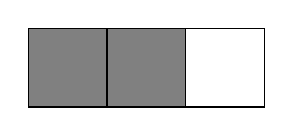
\begin{tikzpicture}
			\draw [draw=black] (3,1) rectangle (0,0);
			\draw [draw=black,fill=gray] (2,1) rectangle (0,0);
			\draw [] (1,1) -- (1,0);
			\draw [] (2,1) -- (2,0);
	\end{tikzpicture}}
	\caption{A relevant proposition.}\label{fig:relevant-p}
\end{subfigure}
\hfill
\begin{subfigure}[t]{.65\linewidth}
	\centering\scalebox{.8}{
		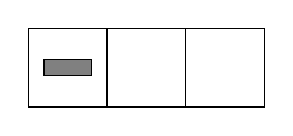
\begin{tikzpicture}
			\draw [draw=black] (3,1) rectangle (0,0);
			\draw [draw=black,fill=gray] (.8,.6) rectangle (.2,.4);
			\draw [] (1,1) -- (1,0);
			\draw [] (2,1) -- (2,0);
	\end{tikzpicture}}
	\hfill\scalebox{.8}{
		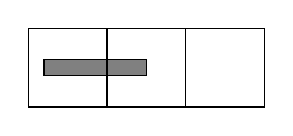
\begin{tikzpicture}
			\draw [draw=black] (3,1) rectangle (0,0);
			\draw [draw=black,fill=gray] (1.5,.6) rectangle (.2,.4);
			\draw [] (1,1) -- (1,0);
			\draw [] (2,1) -- (2,0);
	\end{tikzpicture}}\hfill\scalebox{.8}{
		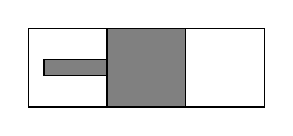
\begin{tikzpicture}
			\draw [draw=black] (3,1) rectangle (0,0);
			\draw [draw=black,fill=gray] (2,1) rectangle (1,0);
			\draw [draw=black,fill=gray] (1,.6) rectangle (.2,.4);
			\draw [] (1,1) -- (1,0);
			\draw [] (2,1) -- (2,0);
	\end{tikzpicture}}
	\caption{Irrelevant propositions.}\label{fig:over-p}
\end{subfigure}
\caption{Various QuD-proposition configurations (proposition defined by the gray area).}\label{fig:qud-p-diagrams}
\end{figure}

This notion is not sensitive to how the proposition at stake packages information: the only relevant(!) factor is whether or not the proposition as a whole can be identified with a union of cells. In other words, the level of granularity conveyed by the proposition is not taken into account when assessing its relevance to the question. This does not seem to match intuitions about what a relevant answer to a question is. For instance, the question set in (\ref{ex:relevant-answers}) strongly suggests a by-country partition of the CS.
\begin{exe}
\ex {In which country did Jo grow up?}
\begin{xlist}
	\ex[] {-- They grew up in France or Belgium.\hfill Relevant}\label{ex:relevant}
	\ex[??] {-- They grew up in Europe (for all I know). \hfill Relevant}\label{ex:relevant-coarse}
	\ex[?] {-- They grew up in Paris. \hfill Irrelevant (overinformative)}\label{ex:overinformative}
	\ex[?] {-- They grew up in Paris or Brussels. \hfill Irrelevant (overinformative)}\label{ex:overinformative-2}
	\ex[??] {-- They speak French natively \hfill More ``strongly'' irrelevant}\label{ex:irrelevant}
\end{xlist}
\label{ex:relevant-answers}
\end{exe}

Given this kind of partition, both (\ref{ex:relevant}) and (\ref{ex:relevant-coarse}) are predicted to be relevant, because France and Belgium are both countries and Europe is also a collection of countries. Yet, (\ref{ex:relevant-coarse}) does not seem so felicitous, at least without hedging. The oddness of this answer seem to come from the fact that \textit{Europe} is ``coarser-grained'' than, say, \textit{France or Belgium}. This can be modeled by saying \textit{Europe} can less straightforwardly be partitioned into country-level cells, than \textit{France or Belgium}. In fact, this is exactly the kind of intuition that Qtrees incorporate: a Qtree for \textit{France or Belgium} is predicted to have a country-level layer, with both \textit{France} and \textit{Belgium} flagged as verifying. A Qtree for \textit{Europe} would stop at the continent-level, the \textit{Europe}-node being verifying. Having a granularity-sensitive notion of Relevance may also help explain why finer-grained, overinformative answers like (\ref{ex:overinformative}) and (\ref{ex:overinformative-2}), are not so infelicitous: they suggest a partition of the CS whose cells (city-level) can all be mapped to a single (country-level) cell of the partition provided by the QuD. (\ref{ex:irrelevant}), which is also overinformative and predicted to be irrelevant, sounds more odd than (\ref{ex:overinformative}) and (\ref{ex:overinformative-2}), because the partition it suggests (\textit{What's Jo's level in French?}) cannot be properly mapped to the partition set by the QuD. For instance, Jo could very well be fluent in French, without having grown up in France. This suggests that granularity-sensitive notion of \textsc{Relevance} should state that a proposition is relevant if it can be partitioned into more specific ``sub-propositions'' (=verifying nodes), s.t. each sub-proposition ``fits'' a cell of the question, i.e., entails it.


We now introduce \textsc{Q-Relevance}, to incorporate a sightly weaker variant of this intuition. Our principle applies incrementally at each step of the Qtree computation process. \textsc{Q-Relevance} targets the verifying nodes of an input Qtree (which play the role of a ``structured'' proposition), and evaluates how these nodes ``fit'' into the output Qtree. A verifying node ``fits'' a Qtree iff it is not cut-out in this Qtree, i.e. iff there is no node of the Qtree that overlaps with it without fully containing it. In other words, no node of the output Qtree should \textit{strictly entail} a verifying node of the input Qtree. This is formalized in (\ref{ex:q-relevance}).

\begin{exe}
\ex {{\textsc{Q-Relevance}}.  Let $X$ and $Y$ be LFs and let $Qtrees(X)$ and $Qtrees(Y)$ be the sets of Qtrees compatible with $X$ and $Y$. Let $\circ$ be a Qtree-level operation, e.g. $\neg$, $\vee$, or $\rightarrow$. Let $C$ be a non-empty partial LF (incremental context). Two cases:
	\begin{itemize}
		\item $C=\circ$, with $\circ$ a unary operation. For any $T \in Qtrees(X)$, $\circ T$ is \textsc{Q-Relevant} with respect to $\circ X$ iff $\forall N \in \mathbb{N}^+(T). \ \neg\exists N' \in \mathbb{N}(\circ T). \ N' \subset N$.
		\item $C = X \circ$, with $\circ$ a binary operation. For any $T \in Qtrees(Y)$, $T_X \circ T_Y$ is \textsc{Q-Relevant} with respect to $X \circ Y$ iff $\forall N \in \mathbb{N}^+(T_Y). \ \neg\exists N' \in \mathbb{N}(T_x \circ T_Y). \ N' \subset N$.
\end{itemize}}\label{ex:q-relevance}
\end{exe}

The predictions of \textsc{Q-Relevance} for our $\lbrace \neg, \vee, \rightarrow\rbrace$ fragment of the language are the following. First, because $\neg$ is structure preserving, we can be sure that all the input verifying nodes are part of the negated output Qtree, satisfying \textsc{Q-Relevance}. Second, because $\vee$ forces well-formed unions of Qtrees (in terms of both structure and verifying nodes), we can be sure that all the input verifying nodes are part of the disjunctive output Qtree, again, satisfying \textsc{Q-Relevance}. The interesting cases arise with $\rightarrow$, because this operation involves intersecting verifying nodes and Qtrees, i.e. performing operations of the form $N \cap T$, with $N$ a verifying node of an antecedent Qtree, and $T$ a consequent Qtree. This kind of operation may affect the nodes of $T$ (in particular, $T$'s verifying nodes) in ways that may violate \textsc{Q-Relevance}. To see this, let us consider a Qtree $T_X\rightarrow T_Y$ compatible with an LF $X \rightarrow Y$. Within $T_X\rightarrow T_Y$, let us focus on a subtree $N\cap T_Y$, with $N \in \mathbb{N}^+(T_X)$. \textsc{Q-Relevance} imposes that for each verifying node in $T_Y$, no node of $N\cap T_Y$ strictly entails it: $\forall N' \in \mathbb{N}^+(T_Y). \neg \exists N'' \in \mathbb{N}(N\cap T_Y). \ N'' \subset N'$. If $N'$ in this formula is incompatible with $N$, then for sure no node $N''$ will strictly entail it. If $N'$ is compatible with $N$, then a violation of \textsc{Q-Relevance} arises as soon as $N \cap N' \subset N'$, i.e. if intersecting $N'$ with $N$ ``shrinks'' $N'$. This holds for any subtree $N\cap T_Y$ of $T_X\rightarrow T_Y$, with $N \in \mathbb{N}^+(T_X)$. Zooming out, this implies that each verifying node of the consequent Qtree compatible with some verifying node of the antecedent Qtree, should be fully preserved in the output.\\

We are now equipped to explain the oddness pattern of the HCs in (\ref{ex:hc}), whose Qtrees are repeated below. \textsc{Q-Relevance} predicts all the Qtrees compatible with the infelicitous HC (\ref{ex:hc-sw}) (cf. Figure \ref{fig:qtrees-if-not-noto-italy}) to be \textsc{Irrelevant}. This is because in each case, the output Qtree contains nodes that strictly entail the verifying \textit{Italy} node of the consequent Qtree: nodes of the form \textit{Italy and not Noto} (in Trees \ref{fig:tree-hc-sw-polar-polar-2} and \ref{fig:tree-hc-sw-polar-wh-2}), or city-level nodes (in Trees \ref{fig:tree-hc-sw-wh-2} and \ref{fig:qtree-if-not-noto-italy-tiered-wh-2}). (\ref{ex:hc-sw}) is thus predicted to be odd, in a way that is consistent with the intuition that raising \textit{Italy} after assuming \textit{not Noto} feels irrelevant to the general question the sentence is trying to answer.

\begin{figure}[H]
\centering
\setlength{\fboxsep}{1pt}
\renewcommand\thefigure{\ref{fig:qtrees-if-not-noto-italy}}
\begin{subfigure}[b]{.22\linewidth}
	\centering
	\scalebox{.7}
	{\begin{forest}for tree={s sep=2mm, inner sep=0, l=0}
			[CS [{Noto}] [{$\neg$Noto} [\fbox{\begin{tabular}{c}
					Italy$\cap\neg$Noto\\
					\textbf{\textcolor{red}{$\subset$ Italy}}
			\end{tabular}}][$\neg$Italy]]]
	\end{forest}}
	\caption{Tree \ref{fig:qtree-not-noto-polar} $\rightarrow$ Tree \ref{fig:qtree-italy-polar}.}\label{fig:tree-hc-sw-polar-polar-2}
\end{subfigure}\hfill
\begin{subfigure}[b]{.22\linewidth}
	\centering
	\scalebox{.7}
	{\begin{forest}for tree={s sep=2mm, inner sep=0, l=0}
			[CS [{Noto}] [{$\neg$Noto} [\fbox{\begin{tabular}{c}
					Italy$\cap\neg$Noto\\
					\textbf{\textcolor{red}{$\subset$ Italy}}
			\end{tabular}}][France] [...]]]
	\end{forest}}
	\caption{Tree \ref{fig:qtree-not-noto-polar} $\rightarrow$ Tree \ref{fig:qtree-italy-wh}.}\label{fig:tree-hc-sw-polar-wh-2}
\end{subfigure}\hfill
\begin{subfigure}[b]{.3\linewidth}
	\centering
	\scalebox{.7}
	{\begin{forest}for tree={s sep=2mm, inner sep=0, l=0}
			[CS [{Noto}] [\fbox{\begin{tabular}{c}
					Rome\\
					\textbf{\textcolor{red}{$\subset$ Italy}}
			\end{tabular}}] [\fbox{\begin{tabular}{c}
					...\\
					\textbf{\textcolor{red}{$\subset$ Italy}}
			\end{tabular}}] [{Paris}] [...]]
	\end{forest}}
	\caption{Tree \ref{fig:qtree-not-noto-wh} $\rightarrow$ Tree \ref{fig:qtree-italy-wh}/\ref{fig:qtree-italy-polar}.}\label{fig:qtree-if-not-noto-italy-wh-wh-2}\label{fig:tree-hc-sw-wh-2}
\end{subfigure}\hfill
\begin{subfigure}[b]{.25\linewidth}
	\centering
	\scalebox{.7}
	{\begin{forest}for tree={s sep=2mm, inner sep=0, l=0}
			[CS [Italy[{Noto}] [\fbox{\begin{tabular}{c}
					Rome\\
					\textbf{\textcolor{red}{$\subset$ Italy}}
			\end{tabular}}] [\fbox{\begin{tabular}{c}
					...\\
					\textbf{\textcolor{red}{$\subset$ Italy}}
			\end{tabular}}]]  [...]]
	\end{forest}}
	\caption{Tree \ref{fig:qtree-not-noto-tiered} $\rightarrow$ Tree \ref{fig:qtree-italy-wh}/\ref{fig:qtree-italy-polar}.}\label{fig:qtree-if-not-noto-italy-tiered-wh-2}
\end{subfigure}
\caption{Qtrees for (\ref{ex:hc-sw})=\#\textit{If SuB29 will not take place in Noto, it will take place in Italy.}}
\end{figure}

Regarding the felicitous HC (\ref{ex:hc-ws}), \textsc{Q-Relevance} predicts some, but crucially not all, of the Qtrees in Figure \ref{fig:qtrees-if-italy-not-noto} to be \textsc{Irrelevant}. Trees \ref{ex:qtree-if-italy-not-noto-polar-polar-2} and \ref{ex:qtree-if-italy-not-noto-wh-polar-2} are \textsc{Irrelevant}, because in both cases, the output Qtree contains nodes of the form \textit{Italy and not Noto}, which strictly entail the verifying \textit{not Noto} node of the consequent Qtree. Trees \ref{ex:qtree-if-italy-not-noto-polar-wh-2} and \ref{ex:qtree-if-italy-not-noto-wh-wh-2} however, do not violate \textsc{Q-Relevance}, because they are constructed from a consequent Qtree for \textit{not Noto} that introduces a city-level partition that perfectly ``fits'' the restriction to \textit{Italy} introduced by the antecedent Qtree, so that no city-node verifying \textit{not Noto} is strictly entailed by a node in the output Qtree. This correctly predicts (\ref{ex:hc-ws}) to be felicitous, in a way that is consistent with the intuition that it is possible to make sense of \textit{not Noto} after assuming \textit{Italy}, granted that \textit{not Noto} discusses a \textit{which city?} kind of question.



\begin{figure}[H]
\setlength{\fboxsep}{1pt}
\renewcommand\thefigure{\ref{fig:qtrees-if-italy-not-noto}}
\centering
\begin{subfigure}[b]{.23\linewidth}
	\centering
	\scalebox{.8}
	{\begin{forest}for tree={s sep=2mm, inner sep=0, l=0}
			[CS [{Italy} [Noto][\fbox{\begin{tabular}{c}
					$\neg$Noto$\cap$Italy\\
					\textbf{\textcolor{red}{$\subset \neg$Noto}}
			\end{tabular}}]] [{$\neg$Italy} ]]
	\end{forest}}
	\caption{Tree \ref{fig:qtree-italy-polar} $\rightarrow$ Tree \ref{fig:qtree-not-noto-polar}.}\label{ex:qtree-if-italy-not-noto-polar-polar-2}
\end{subfigure}\hfill
\begin{subfigure}[b]{.25\linewidth}
	\centering
	\scalebox{.8}
	{\begin{forest}for tree={s sep=2mm, inner sep=0, l=0}
			[CS [{Italy} [{Noto}] [\fbox{Rome}] [\fbox{...}]] [{$\neg$Italy} ]]
	\end{forest}}
	\caption{Tree \ref{fig:qtree-italy-polar} $\rightarrow$ Tree \ref{fig:qtree-not-noto-wh}/\ref{fig:qtree-not-noto-tiered}.}\label{ex:qtree-if-italy-not-noto-polar-wh-2}
\end{subfigure}
\hfill
\begin{subfigure}[b]{.25\linewidth}
	\centering
	\scalebox{.8}
	{\begin{forest}for tree={s sep=2mm, inner sep=0, l=0}
			[CS [Italy[Noto][\fbox{\begin{tabular}{c}
					$\neg$Noto$\cap$Italy\\
					\textbf{\textcolor{red}{$\subset \neg$Noto}}
			\end{tabular}}]] [France] [...]]
	\end{forest}}
	\caption{Tree \ref{fig:qtree-italy-wh} $\rightarrow$ Tree \ref{fig:qtree-not-noto-polar}.}\label{ex:qtree-if-italy-not-noto-wh-polar-2}
\end{subfigure}\hfill
\begin{subfigure}[b]{.25\linewidth}
	\centering
	\scalebox{.8}
	{\begin{forest}for tree={s sep=2mm, inner sep=0, l=0}
			[CS [Italy[{Noto}] [\fbox{Rome}] [\fbox{...}]] [France] [...] ]
	\end{forest}}
	\caption{Tree \ref{fig:qtree-italy-wh} $\rightarrow$ Tree \ref{fig:qtree-not-noto-wh}/\ref{fig:qtree-not-noto-tiered}.}\label{ex:qtree-if-italy-not-noto-wh-wh-2}
\end{subfigure}
\caption{Qtrees for (\ref{ex:hc-ws})=\textit{If SuB29 will take place in Italy, it will not take place in Noto.}}\label{ex:qtree-if-italy-not-noto-2}
\end{figure}

\section{Extensions}\label{sec:ccl}
We developed an account of Hurford Sentences based on implicit QuDs and constraints on their derivation. This framework captured the challenging contrast between HDs, which are infelicitous regardless of the order of the disjuncts, and HCs, whose felicity profile seems sensitive to granularity considerations. We also sketched how this model could capture Long-Distance HDs.

\subsection{Compatible, non-entailing disjuncts}


Interestingly, the model extends its scope to HDs with merely compatible disjuncts \citep{Singh2008b}, exemplified in (\ref{ex:hd-compatible}).

\begin{exe}
\ex[\#] {SuB29 will take place in the Basque country\footnotemark{} or France.}\label{ex:hd-compatible}
\end{exe} 
\footnotetext{Given that the Basque country encompasses Northern Central Spain and southwestern France, it is compatible with \textit{France}, without entailment in any direction.}

In (\ref{ex:hd-compatible}) the first disjunct suggests a by-region partition, such that the Basque country represents a (verifying) leaf; while the second disjunct suggests a by-country partition, such that France represents a (verifying) leaf. The relevant Qtrees are built in Figure \ref{fig:qtrees-compat}.

\begin{figure}[H]
\centering
\begin{subfigure}[b]{.55\linewidth}
	\centering
	\scalebox{.8}{
		\begin{forest}for tree={s sep=2mm, inner sep=0, l=0}
			[CS [\fbox{Basque}] [$\neg${Basque}]]
	\end{forest}}
	\hfill
	\scalebox{.8}{
		\begin{forest}for tree={s sep=2mm, inner sep=0, l=0}
			[CS [\fbox{Basque country}] [Navarre] [Midi] [...]]
	\end{forest}}
	\caption{Qtrees for \textit{SuB29 will take place in the Basque country}, given principles (\ref{ex:qtree-simplex-def}\ref{pt:simplex-qtree-polar}) (left tree) or (\ref{ex:qtree-simplex-def}\ref{pt:simplex-qtree-wh}) (right tree).}\label{fig:qtrees-basque}
\end{subfigure}\hfill
\begin{subfigure}[b]{.4\linewidth}
	\centering
	\scalebox{.8}{
		\begin{forest}for tree={s sep=2mm, inner sep=0, l=0}
			[CS [\fbox{France}] [$\neg$France]]
	\end{forest}}\hfill
	\scalebox{.8}{
		\begin{forest}for tree={s sep=2mm, inner sep=0, l=0}
			[CS [\fbox{France}] [Spain] [...]]
	\end{forest}}
	\caption{Qtrees for \textit{SuB29 will take place in France}, given principles (\ref{ex:qtree-simplex-def}\ref{pt:simplex-qtree-polar}) (left tree) or (\ref{ex:qtree-simplex-def}\ref{pt:simplex-qtree-wh}) (right tree).}\label{fig:qtrees-france}
\end{subfigure}\hfill
\caption{Possible Qtrees for the disjuncts of (\ref{ex:hd-compatible}).}\label{fig:qtrees-compat}
\end{figure}


Can  a disjunctive Qtree be built for (\ref{ex:hd-compatible})? It turns out that the trees in Figure \ref{fig:qtrees-basque} cannot be properly disjoined with any of those in Figure \ref{fig:qtrees-france}, due to the fact that they introduce different, parallel partitionings. The only remaining way to disjoin Qtrees associated with each disjunct of (\ref{ex:hd-compatible}), would be to create a tiered Qtree for \textit{SuB29 will take place in the Basque country}, involving a by-country layer (\textit{via} principle (\ref{ex:qtree-simplex-def}\ref{pt:simplex-qtree-tiered})). But a problem arises in the formation of such a Qtree. Given that \textit{p}=\textit{SuB29 will take place in the Basque country} does not entail that SuB29 will place in any single specific country, it is impossible to create a $p$-chain containing a country-level alternative to $p$. Consequently, no Qtree generated from \textit{SuB29 will take place in the Basque country} using principle (\ref{ex:qtree-simplex-def}\ref{pt:simplex-qtree-tiered}) will contain a by-country layer. To summarize, we predict a sentence like (\ref{ex:hd-compatible}) to be odd because it features compatible disjuncts with incomparable degrees of granularity, which cannot lead to any well-formed disjunctive Qtree.

However, HC-variants of (\ref{ex:hd-compatible}) are predicted by our model to be odd regardless of the ordering of the antecedent and consequent, because Qtrees evoked by \textit{France} and Qtrees evoked by \textit{the Basque country} are not in any kind of refinement relation. This prediction is not empirically borne out, as shown in (\ref{ex:hc-compatible}).

\begin{exe}
\ex \label{ex:hc-compatible}
\begin{xlist}
	\ex[?] {If SuB29 will take place in France, it will take place in the Basque country.}\label{ex:hc-compatible-ws}
	\ex[\#] {If SuB29 will take place in the Basque country, it will take place in France.}\label{ex:hc-compatible-sw}
\end{xlist}
\end{exe}

Within our framework, the contrast in (\ref{ex:hc-compatible}) suggests that it is somehow easier to split the set of \textit{Basque country} worlds into French and Spanish subsets (in order to satisfy \textsc{Q-Relevance} in \ref{ex:hc-compatible-ws}), than to split the set of \textit{France} worlds into Basque and non-Basque subsets (in order to satisfy \textsc{Q-Relevance} in \ref{ex:hc-compatible-sw}). Future work should investigate when, and how such coercion operations on Qtrees can take place.\\





\iffalse
\begin{subfigure}[b]{.33\linewidth}
\centering
\scalebox{.8}{
	\begin{forest}for tree={s sep=7mm, inner sep=0, l=0}
		[CS [{France} [Midi] [~]] [Spain [~] [Navarre]] [...]]
		\node[draw,align=center] at (-.75,-2.3) {Basque\\country};
\end{forest}}
\caption{A tentative Qtree for \textit{Sub will take place in the Basque country}, given principle (\ref{ex:qtree-simplex-def}\ref{pt:simplex-qtree-tiered})}\label{fig:qtree-basque-tiered}
\end{subfigure}
\fi

\subsection{``Long-Distance'' HCs}
In this section, we explore how our QuD-informed view of redundancy captures two kinds of ``Long-Distance'' variants of HCs: those derived from LDHDs \textit{via} the \textit{or-to-if} tautology; and those derived by applying the ``Long Distance'' recipe directly to HCs. 


\subsubsection{LDHCs derived from LDHDs}

Recall that ``Long Distance'' HDs (\textbf{LDHDs}, \citenp{Marty2022}) are obtained from standard HDs of the form \p{} $\vee$ \pplus{} by further disjoining \pplus{} with a proposition \r{}, s.t. \pplus{} $\vee$ \r{} is not redundant, and no longer entails \p. This can be done by choosing \r{} to contradict \pplus{} and \p{}. Such constructions have been argued to be deviant, despite the fact that none of their disjuncts are in an entailment relation (and thus satisfy the traditional, non-explanatory version of Hurford's Constraint). (\ref{ex:ldhd-pos}) illustrates a classic LDHD: \textit{Europe} entails \textit{France}, and \textit{France} is further disjoined with \textit{New York}, that is incompatible with \textit{Europe} -- making the two main disjuncts compatible, but non-entailing.  (\ref{ex:ldhd-neg}) illustrates a perhaps more degenerate case of LDHD: the weak disjunct, \textit{not France}, takes the form of the negation of the stronger disjunct of (\ref{ex:ldhd-pos}); the stronger disjunct, \textit{not Europe}, takes the form of the negation of the weak disjunct of (\ref{ex:ldhd-pos}); and the extra proposition disjoined with it (\textit{Paris}), is chosen to be incompatible with \textit{not France} and \textit{not Europe}. Note that the kind of variable change we described here, was already used to construct simple infelicitous HCs like (\ref{ex:hc-ns-w}).

\begin{exe}
	\exr{ex:ldhd}
	\begin{xlist}
		\ex[\#] {Jo either studied in \textcolor{blue}{Europe}, or in \textcolor{orange}{France} or in \textcolor{green}{New York}.
			\hfill \p{} $\vee$ (\pplus{} $\vee$ \r)}\label{ex:ldhd-pos}
		\ex[\#] {Jo either does\textcolor{blue}{n't study in France}, or \textcolor{orange}{not in Europe} or in \textcolor{green}{Paris}.	\hfill \textbf{\textcolor{blue}{q}} $\vee$ (\textcolor{orange}{\textbf{q}$^+$} $\vee$ \r)\\
			with: \textbf{\textcolor{blue}{q}} := $\neg$\pplus; \textcolor{orange}{\textbf{q}$^+$} := $\neg$\p }\label{ex:ldhd-neg}
	\end{xlist}
\end{exe}

We think that both (\ref{ex:ldhd-pos}) and (\ref{ex:ldhd-neg}) are degraded -- which is in itself interesting because SR predicts (\ref{ex:ldhd-neg}) to be fine.

\begin{exe}
	\ex 
	\begin{xlist}
		\ex {(\ref{ex:ldhd-pos})=\p{} $\vee$ (\pplus{} $\vee$ \r) is SR.\\
			C = \pplus. $\forall D. $ \p{} $\vee$ ((\pplus{}$\wedge$ $D$) $\vee$ \r) $\equiv$ \p{} $\vee$ ((\pplus{}$\vee$ \r) $\wedge$ ($D$ $\vee$ \r)) $\equiv$ (\p{} $\vee$ \r) $\wedge$ (\p{} $\vee$ $D$ $\vee$ \r) $\equiv$ \p{} $\vee$ \r}
		\ex {(\ref{ex:ldhd-neg}) = $\neg$\pplus{} $\vee$ ($\neg$\p{} $\vee$ \r) is not SR.\\
			C = $\neg$\pplus. Take $D = \top$.\\
			$\neg$(\pplus{} $\wedge$ $D$) $\vee$ ($\neg$\p{} $\vee$ \r) $\equiv$ $\neg$\pplus{} $\vee$ ($\neg$\p{} $\vee$ \r) $\equiv$ $\neg$\pplus{} $\vee$ \r{} $\not\equiv$ $\neg$\p{} $\vee$ \r\\
			C = $\neg$\p. Take $D = \bot$.\\
			$\neg$\pplus{} $\vee$ ($\neg$(\p{} $\wedge$ $D$) $\vee$ \r) $\equiv$ $\neg$\pplus{} $\vee$ ($\top$ $\vee$ \r) $\equiv$ $\top$ $\not\equiv$ $\neg$\pplus{} $\vee$ \r\\
			C = \r. Take $D = \top$.\\
			$\neg$\pplus{} $\vee$ ($\neg$\p{} $\vee$ (\r{} $\wedge$ $D$)) $\equiv$ $\neg$\pplus{} $\vee$ \r{} $\not\equiv$ $\neg$\pplus $\equiv$ $\neg$\pplus{} $\vee$ $\neg$\p{}\\
			C = ($\neg$\p{} $\vee$ \r). Take $D = \top$.\\
			$\neg$\pplus{} $\vee$ (($\neg$\p{} $\wedge$ $D$) $\vee$ (\r{} $\wedge$ $D$)) $\equiv$ $\neg$\pplus{} $\vee$ ($\neg$\p{} $\vee$ \r) $\equiv$ $\neg$\pplus{} $\vee$ \r{} $\not\equiv$ $\neg$\pplus
			
		}
	\end{xlist}
	
\end{exe}

Interestingly, turning the LDHDs in (\ref{ex:ldhd}) into conditionals maintains infelicity, as shown in (\ref{ex:ldhc}).

\begin{exe}
	\exr{ex:ldhc}
	\begin{xlist}
		\ex[\#] {If Jo did not study in \textcolor{blue}{Europe}, she studied in \textcolor{orange}{France} or in \textcolor{green}{New York}.}
		\ex[\#] {If Jo studied in \textcolor{blue}{France}, she did not study \textcolor{orange}{in Europe} or she studied in \textcolor{green}{Paris}.}
	\end{xlist}
\end{exe}

We proceed to show that both (\ref{ex:ldhc-pos}) and (\ref{ex:ldhc-neg}) are \textsc{Q-Redundant}. \textsc{Q-Redundancy}, as defined in Chapter \ref{chap:hurford-sentences}, states that a Qtree $T$ paired with a specific LF $X$ is deviant iff the $T$ is equivalent to a tree $T'$ compatible with a simplification of $X$. (\ref{ex:ldhc-pos}) is then \textsc{Q-Redundant} because any Qtree it evokes is also evoked by (\ref{ex:ldhc-pos-simplification}); and (\ref{ex:ldhc-neg}) is \textsc{Q-Redundant} as well, because any Qtree it evokes is also evoked by (\ref{ex:ldhc-neg-simplification}).

\begin{exe}
	\ex\label{ex:ldhc-simplifications}
	\begin{xlist}
		\ex[] {If Jo did not study in \textcolor{blue}{Europe}, she studied in \textcolor{green}{New York}.}\label{ex:ldhc-pos-simplification}
		\ex[] {If Jo studied in \textcolor{blue}{France}, she studied in \textcolor{green}{Paris}.}\label{ex:ldhc-neg-simplification}
	\end{xlist}
\end{exe}

We start with (\ref{ex:ldhc-pos}). The possible Qtrees evoked by its antecedent ($\neg$\textit{Europe}) are depth-1 Qtrees whose leaves are $\lbrace$\textit{Europe}, $\neg$\textit{Europe}$\rbrace$, or continent-level alternatives $\lbrace$\textit{Europe}, \textit{Africa}, \textit{Asia}, ...$\rbrace$. ``Tiered'' Qtrees are unlikely, since coarser-grained alternatives to continent-level locations are themselves unlikely to be salient. In each possible Qtree, the leaves incompatible with \textit{Europe} are flagged as verifying (effect of negation). This is summarized in Figure \ref{trees:not-Europe}.

\begin{figure}[H]
	\centering
	\begin{subfigure}[b]{.3\linewidth}
		\centering
		\scalebox{1}{
			\begin{forest}
				[CS[Europe][\fbox{$\neg$Europe}]]
			\end{forest}
		}
		\caption{}\label{tree:not-europe-polar}
	\end{subfigure}
	\qquad
	\begin{subfigure}[b]{.3\linewidth}
		\centering
		\scalebox{1}{
			\begin{forest}
				[CS[Europe][\fbox{America}][\fbox{Africa}][\fbox{...}]]
			\end{forest}
		}
		\caption{}\label{tree:not-europe-wh}
	\end{subfigure}
	\caption{Qtrees for \textit{Jo did not study in \textcolor{blue}{\textbf{Europe}}.}}\label{trees:not-Europe}
\end{figure}

The consequent of (\ref{ex:ldhc-pos}) is disjunctive, and therefore results from the well-formed union of Qtrees evoked by its two disjuncts (\textit{France} and \textit{New York}). Possible Qtrees for \textit{France} (already computed in section \ref{sec:qtrees-scalemates-non-scalemates}), are repeated in Figure \ref{trees:france-2}; possible Qtrees for \textit{New York} can be computed in a way that is strictly analogous to Qtrees for \textit{Paris} (as done in section \ref{sec:qtrees-scalemates-non-scalemates}), and are thus given in Figure \ref{trees:new-york}.
\begin{figure}[H]
	\centering
	\begin{subfigure}[b]{.3\linewidth}
		\centering
		\begin{forest}
			[CS[\bfbox{France}][$\neg$France]]
		\end{forest}
		\caption{}\label{tree:france-polar-2}
	\end{subfigure}
	\qquad
	\begin{subfigure}[b]{.3\linewidth}
		\centering
		\begin{forest}
			[CS[\bfbox{France}][US][...]]
		\end{forest}
		\caption{}\label{tree:france-wh-2}
	\end{subfigure}
	\caption{Qtrees for \textit{Jo studied in \textbf{\textcolor{blue}{France}}}.} \label{trees:france-2}
\end{figure}

\begin{figure}[H]
	\centering
	\begin{subfigure}[b]{.3\linewidth}
		\centering
		\scalebox{1}{
			\begin{forest}
				for tree={s sep=2mm, inner sep=0, l=0}
				[CS[\gfbox{New York}][$\neg$New York]]
		\end{forest}}
		\caption{}\label{tree:new-york-polar}
	\end{subfigure}
	\hfill
	\begin{subfigure}[b]{.3\linewidth}
		\centering
		\scalebox{1}{
			\begin{forest}
				for tree={s sep=2mm, inner sep=0, l=0}
				[CS[\gfbox{New York}][Boston][Paris][...]]
		\end{forest}}
		\caption{}\label{tree:new-york-wh}
	\end{subfigure}\hfill
	\begin{subfigure}[b]{.3\linewidth}
		\centering
		\scalebox{1}{
			\begin{forest}
				for tree={s sep=2mm, inner sep=0, l=0}
				[CS[France[{Paris}][...]][US[\gfbox{New York}][Boston]][...]]
		\end{forest}}
		\caption{}\label{tree:new-york-tiered}
	\end{subfigure}
	
	
	\caption{Qtrees for \textit{Jo studied in \textbf{\textcolor{green}{New York}}.}}\label{trees:new-york}
\end{figure}

Unioning Qtrees from Figures \ref{trees:france-2} and \ref{trees:new-york} can be done in only one way: using Tree \ref{tree:france-wh-2} for \textit{France}, and Tree \ref{tree:new-york-tiered}, for \textit{New York}. This yields the Qtree in Figure \ref{tree:france-or-new-york}.

\begin{figure}[H]
	\centering
	\scalebox{1}{
		\begin{forest}
			for tree={s sep=2mm, inner sep=0, l=0}
			[CS[\fbox{France}[{Paris}][...]][US[\fbox{New York}][Boston][...]][...]]
	\end{forest}}
	\caption{Qtree for \textit{Jo studied in \textcolor{orange}{\textbf{France}} or in \textcolor{green}{\textbf{New York}}}.}\label{tree:france-or-new-york}
\end{figure}

Now that Qtrees for the antecedent and the consequent of (\ref{ex:ldhc-pos}) are derived, we can combine them to form a Qtree for the whole conditional, by taking the antecedent Qtrees from Figure \ref{trees:not-Europe} and replacing their verifying nodes (anything non Europe) by their intersection with the consequent Qtree from Figure \ref{tree:france-or-new-york}. This yields the Qtrees in Figure \ref{trees:if-not-Europe-then-france-or-new-york}. 

\begin{figure}[H]
	\centering
	\begin{subfigure}[b]{.45\linewidth}
		\centering
		\scalebox{1}{
			\begin{forest}
				for tree={s sep=2mm, inner sep=0, l=0}
				[CS[Europe][{$\neg$Europe} [US[\fbox{New York}][Boston][...]][Japan[...]][...]]]
			\end{forest}
		}
		\caption{}
	\end{subfigure}
	\hfill
	\begin{subfigure}[b]{.45\linewidth}
		\centering
		\scalebox{1}{
			\begin{forest}
				for tree={s sep=2mm, inner sep=0, l=0}
				[CS[Europe][{America}[US[\fbox{New York}][Boston][...]][...]][{Africa}[...]][{...}]]
			\end{forest}
		}
		\caption{}
	\end{subfigure}
	\caption{Qtrees for (\ref{ex:ldhc-pos}) = \textit{If Jo did not study in \textcolor{blue}{\textbf{Europe}}, she studied in \textcolor{orange}{\textbf{France}} or in \textcolor{green}{\textbf{New York}}.}}\label{trees:if-not-Europe-then-france-or-new-york}
\end{figure}

Crucially, the intersection operation between the consequent Qtree in Figure \ref{tree:france-or-new-york}, and the non-Europe nodes in the Qtrees from Figure \ref{trees:not-Europe}, discarded the sections of the consequent Qtree that had to do with \textit{France}. This does not violate \textsc{Q-Relevance}, but instead, causes the output Qtrees to be identical (and hence, equivalent) to Qtrees evoked by a formal simplification of (\ref{ex:ldhc-pos}) that does not feature \textit{France} as a disjunct in its consequent -- namely, (\ref{ex:ldhc-pos-simplification}). Any Qtree derived from (\ref{ex:ldhc-pos}) is thus \textsc{Q-Redundant}, and as a result, we correctly predict (\ref{ex:ldhc-pos}) to be infelicitous.\\

We can now move on to the case of (\ref{ex:ldhc-neg}). The possible Qtrees evoked by its antecedent (France), are already given in Figure \ref{trees:france-2}.


The consequent of (\ref{ex:ldhc-neg}) is disjunctive, and therefore results from the well-formed union of Qtrees evoked by its two disjuncts ($\neg$\textit{Europe} and \textit{Paris}). Possible Qtrees for $\neg$\textit{Europe} are already given in Figure \ref{trees:not-Europe}. Possible Qtrees for \textit{Paris} are given in Figure \ref{trees:paris}.

\begin{figure}[H]
	\centering
	\begin{subfigure}[b]{.3\linewidth}
		\centering
		\scalebox{1}{
			\begin{forest}
				for tree={s sep=2mm, inner sep=0, l=0}
				[CS[\ofbox{Paris}][$\neg$Paris]]
		\end{forest}}
		\caption{}\label{tree:paris-polar}
	\end{subfigure}
	\hfill
	\begin{subfigure}[b]{.3\linewidth}
		\centering
		\scalebox{1}{
			\begin{forest}
				for tree={s sep=2mm, inner sep=0, l=0}
				[CS[\ofbox{Paris}][Nice][London][...]]
		\end{forest}}
		\caption{}\label{tree:paris-wh}
	\end{subfigure}\hfill
	\begin{subfigure}[b]{.3\linewidth}
		\centering
		\scalebox{1}{
			\begin{forest}
				for tree={s sep=2mm, inner sep=0, l=0}
				[CS[France[\ofbox{Paris}][Nice][...]][UK[London][...]][...]]
		\end{forest}}
		\caption{}\label{tree:paris-tiered}
	\end{subfigure}
	\begin{subfigure}[b]{.3\linewidth}
		\centering
		\scalebox{1}{
			\begin{forest}
				for tree={s sep=2mm, inner sep=0, l=0}
				[CS[Europe[France[\fbox{Paris}][Nice][...]][UK[London][...]]][America[...]][...]]
		\end{forest}}
		\caption{}\label{tree:paris-tiered-tiered}
	\end{subfigure}
	
	
	\caption{Qtrees for \textit{Jo studied in \textbf{\textcolor{orange}{Paris}}.}}\label{trees:paris}
\end{figure}

Unioning Qtrees from Figures \ref{trees:not-Europe} and \ref{trees:paris} can be done in only one way: using Tree \ref{tree:not-europe-wh} for $\neg$\textit{Europe}, and Tree \ref{tree:paris-tiered-tiered}, for \textit{Paris}. This yields the Qtree in Figure \ref{tree:not-europe-or-paris}.

\begin{figure}[H]
	\centering
	\scalebox{1}{
		\begin{forest}
			for tree={s sep=2mm, inner sep=0, l=0}
			[CS[Europe[France[\fbox{Paris}][Nice][...]][UK[London][...]]][\fbox{America}[{...}]][\fbox{...}]]
	\end{forest}}
	\caption{Qtrees for \textit{Jo did not study in \textbf{\textcolor{blue}{Europe}} or studied in \textbf{\textcolor{orange}{Paris}}.}}\label{tree:not-europe-or-paris}
\end{figure}

Now that Qtrees for the antecedent and the consequent of (\ref{ex:ldhc-neg}) are derived, we can combine them to form a Qtree for the whole conditional, by taking the antecedent Qtrees from Figure \ref{trees:france-2} and replacing their verifying nodes (\textit{France} nodes) by their intersection with the consequent Qtree from Figure \ref{tree:not-europe-or-paris}. This yields the Qtrees in Figure \ref{trees:if-france-then-not-europe-or-paris}. 

\begin{figure}[H]
	\centering
	\begin{subfigure}[b]{.3\linewidth}
		\centering
		\begin{forest}
			[CS[{France}[\fbox{Paris}][Nice][...]][$\neg$France]]
		\end{forest}
		\caption{}
	\end{subfigure}
	\qquad
	\begin{subfigure}[b]{.3\linewidth}
		\centering
		\begin{forest}
			[CS[{France}[\fbox{Paris}][Nice][...]][US][...]]
		\end{forest}
		\caption{}
	\end{subfigure}
	\caption{Qtrees for (\ref{ex:ldhc-neg}) = \textit{If Jo studied in \textcolor{blue}{\textbf{France}}, she did not study in \textcolor{orange}{\textbf{Europe}} or she studied in \textcolor{green}{\textbf{Paris}}.}} \label{trees:if-france-then-not-europe-or-paris}
\end{figure}

Crucially, the intersection operation between the consequent Qtree in Figure \ref{tree:not-europe-or-paris}, and the \textit{France} nodes in the Qtrees from Figure \ref{trees:france-2}, discarded the sections of the consequent Qtree that had to do with $\neg$\textit{Europe}. This does not violate \textsc{Q-Relevance}, but instead, causes the output Qtrees to be identical (and hence, equivalent) to Qtrees evoked by a formal simplification of (\ref{ex:ldhc-neg}) that does not feature $\neg$\textit{Europe} as a disjunct in its consequent -- namely, (\ref{ex:ldhc-neg-simplification}). Any Qtree derived from (\ref{ex:ldhc-neg}) is thus \textsc{Q-Redundant}, and as a result, we correctly predict (\ref{ex:ldhc-neg}) to be infelicitous.\\

In sum, \textsc{Q-Redundancy} predicts both kinds of LDHCs derived from LDHDs via the \textit{or-to-if} tautology to be infelicitous, in line with pre-theoretical intuitions about these sentences.




\subsubsection{LDHCs derived from HCs}

This reasoning extends to the LDHCs (\ref{ex:ldhc-w-ns}) and (\ref{ex:ldhc-ns-w}), whose trees are given in Fig. \ref{fig:ldhc-non-scalar-w-ns} and \ref{fig:ldhc-non-scalar-ns-w}. For (\ref{ex:ldhc-w-ns}), \textsc{Q-Relevance} is satisfied because none of the verifying leaves from the consequent Qtree (cities different from Paris and Brussels) are cut across in the output Qtree. The feeling of redundancy in (\ref{ex:ldhc-w-ns}) may come from the fact removing \textit{Brussels} from the sentence leads to the same overall meaning and Qtree.\footnote{Following \citet{HenotMortier2024a,HenotMortier2024b}, this implies that (\ref{ex:ldhc-w-ns}) is \textsc{Q-Redundant}.} For (\ref{ex:ldhc-ns-w}), \textsc{Q-Relevance} is violated because the compatible \textit{France} leaf from the consequent Qtree cannot ``fit'' into the city-level nodes introduced by the antecedent.


\begin{minipage}{.45\linewidth}
	\centering
	\begin{figure}[H]
		\centering
		\scalebox{.7}{
			\begin{forest}
				[CS[FR[Paris][\fbox{Nice}][\fbox{...}]][$\neg$FR/UK]]
		\end{forest}}
		\caption{Qtree for (\ref{ex:ldhc-w-ns}).}\label{fig:ldhc-non-scalar-w-ns}
	\end{figure}
\end{minipage}
\hfill
\begin{minipage}{.45\linewidth}
	\centering
	\begin{figure}[H]
		\centering
		\scalebox{.7}{
			\begin{forest}
				[CS[Paris][Brussels][\fbox{\begin{tabular}{c}
						FR$\wedge$Nice\\
						\textcolor{red}{$\subset$ FR}
				\end{tabular}}][...]]
		\end{forest}}
		\caption{Qtree for (\ref{ex:ldhc-ns-w}).}\label{fig:ldhc-non-scalar-ns-w}
	\end{figure}
\end{minipage}





An argument against this view comes from Long-Distance HCs (henceforth LDHC). Such structures, inspired from Long-Distance HDs (\cite{Marty2022}) and exemplified in (\ref{ex:ldhc}), are derived from (\ref{ex:hc-s}) by further disjoining \pplus{} with a proposition \r{} taken to be incompatible with \p. 


\begin{exe}
	\ex\label{ex:ldhc-surface}
	\begin{xlist}
		\ex[?] {If Jo studied in \textcolor{blue}{France} she didn't study in \textcolor{orange}{Paris} or \textcolor{green}{Brussels}.\hfill \p$\rightarrow\neg$(\pplus$\vee$\r)}\label{ex:ldhc-w-ns}
		\ex[\#] {If Jo didn't study in \textcolor{orange}{Paris} or \textcolor{green}{Brussels} she studied in \textcolor{blue}{France}.\hfill $\neg$(\pplus$\vee$\r)$\rightarrow$\p}\label{ex:ldhc-ns-w}
	\end{xlist}
\end{exe}

Felicity-wise, LDHCs seem quite degraded: (\ref{ex:ldhc-w-ns}) is felt to convey the same kind of information twice (because having studied in France contextually entails not having studied in Brussels), while (\ref{ex:ldhc-ns-w})'s consequent feels independent from the subject matter raised by the antecedent. Yet neither (\ref{ex:ldhc-w-ns}) nor (\ref{ex:ldhc-ns-w}) are predicted to be SR, due to the presence of \r{}.

\begin{exe}
	\ex (\ref{ex:ldhc-w-ns}) is not SR
	\begin{xlist}
		\ex {C = \pplus{} $\vee$\r. Take $D = \top$.\\\p{} $\rightarrow$ $\neg$((\pplus{} $\vee$ \r) $\wedge$ $D$) $\equiv$ \p{} $\rightarrow$ $\neg$(\pplus{} $\vee$ \r) $\not\equiv$ \p}
		\ex {C = \p. Take $D = \bot$.\\
			(\p{} $\wedge$ $D$) $\rightarrow$ $\neg$(\pplus{}$\vee$ \r) $\equiv$ (\p{} $\wedge$ $\bot$) $\rightarrow$ $\neg$(\pplus{}$\vee$ \r) $\equiv$ $\bot$ $\rightarrow$ $\neg$(\pplus{}$\vee$ \r) $\equiv$ $\top$ $\not\equiv$ $\neg$(\pplus{}$\vee$\r)} 
		\ex {C = \pplus. Take $D = \top$.\\
			\p{} $\rightarrow$ $\neg$((\pplus{}$\wedge$ $D$)$\vee$ \r) $\equiv$ \p{} $\rightarrow$ $\neg$(\pplus{}$\vee$ \r) $\equiv$ $\neg$\p{} $\vee$ ($\neg$\pplus{}$\wedge$$\neg$\r) $\equiv$ $\neg$\pplus{}$\wedge$(\p{}$\rightarrow$$\neg$\r) $\not\equiv$ \p{}$\rightarrow$$\neg$\r}
		\ex {C = \r. Take $D = \top$.\\
			\p{} $\rightarrow$ $\neg$(\pplus{}$\vee$(\r{} $\wedge$ $D$)) $\equiv$ \p{} $\rightarrow$ $\neg$(\pplus{}$\vee$ \r) $\equiv$ $\neg$\p{} $\vee$ ($\neg$\pplus{}$\wedge$$\neg$\r) $\equiv$ $\neg$\pplus{}$\wedge$(\p{}$\rightarrow$$\neg$\r) $\not\equiv$ \p{}$\rightarrow$$\neg$\pplus}
		\label{ex:sr-ldhc-ws}
	\end{xlist}
	\ex (\ref{ex:ldhc-ns-w}) is not SR
	\begin{xlist}
		\ex {C = \pplus{} $\vee$ \r. Take $D = \top$.\\ $\neg$((\pplus{} $\vee$ \r) $\wedge$ $D$) $\rightarrow$ \p{} $\equiv$ $\neg$(\pplus{} $\vee$ \r) $\rightarrow$ \p{} $\equiv$ \r{} $\vee$ \p{} $\not\equiv$ \p}
		\ex {C = \p. Take $D = \bot$.\\
			$\neg$(\pplus{}$\vee$ \r) $\rightarrow$ (\p{} $\wedge$ $D$) $\equiv$  $\neg$(\pplus{}$\vee$ \r)$\rightarrow$(\p{} $\wedge$ $\bot$)  $\equiv$ \pplus{}$\vee$ \r{} $\vee$ $\bot$ $\equiv$ \pplus{}$\vee$ \r{} $\not\equiv$ $\neg$(\pplus{}$\vee$\r)}
		\ex {C = \pplus. Take $D = \bot$.\\
			$\neg$((\pplus{} $\wedge$ $D$)$\vee$ \r) $\rightarrow$ \p{}  $\equiv$  $\neg$(\pplus{}$\vee$ \r)$\rightarrow$ \p{} $\equiv$ \pplus{}$\vee$ \r{} $\vee$ $\bot$ $\equiv$ \pplus{}$\vee$ \r{} $\not\equiv$ $\neg$(\pplus{}$\vee$\r)} \label{ex:sr-ldhc-sw}
	\end{xlist}
\end{exe}

\begin{exe}
	\ex 
	\begin{xlist}
		\ex[\#] {Jo studied in \textcolor{orange}{Paris} or \textcolor{green}{Brussels} or she studied in \textcolor{blue}{France}. \hfill (\pplus$\vee$\r) $\vee$ \p}\label{ex:ldhd-s-w}
		\ex[\#] {Jo studied in \textcolor{blue}{France} or she studied in \textcolor{orange}{Paris} or \textcolor{green}{Brussels}.\hfill \p{} $\vee$ (\pplus$\vee$\r)}\label{ex:ldhd-w-s}
	\end{xlist}
\end{exe}



\section{Outlook}

Beyond the Hurford Sentences used as a case study for this chapter, our model of implicit QuDs raises a variety of questions: what distinguishes non-scalar from scalar alternatives when it comes to Qtree computation? How do Qtrees interact with presuppositions, and with operators such as \textit{exh}, \textit{only}, \textit{at least}? Can we extend the model to (incrementally) predict the shape of the follow-up questions \textit{raised} by sentences? Chapters 4 and 5 will deal with some of these questions. The next Chapter presents another use case for our model of QuDs and the concept of \textsc{Q-Redudancy}. Crucially, the data presented in the next Chapter (variations of the structure $p \vee p \vee q$ based on the \textit{or-to-if} tautology), represent a challenge for \citeauthor{Kalomoiros2024}'s account, as well as other accounts of pragmatic oddness, \textsc{Redundancy}-based, or not.



 %compared previous chapter to existing accounts
%\sloppy
	

\chapter{Scalarity, information structure and Relevance in Hurford Conditionals}\label{chap:scalarity}

\begin{center}
	\textbf{Abstract}
\end{center}

\begin{small}
	Hurford Conditionals (HCs) involving scalemates appear felicitous, despite the fact that \textit{exh} is not predicted to rescue such structures from redundancy constraints previously introduced in the literature. We show that \textsc{Q-Relevance}, as introduced in Chapter \ref{chap:hurford-sentences}, can explain this pattern, modulo the intuitive assumption that scalar items can evoke fine-grained enough questions (generated by their scalemates) out-of-the-blue, while non-scalar items conveying different degrees of granularity cannot.
\end{small}
	\section{Hurford Sentences and scalar implicatures}
	In Chapter \ref{chap:hurford-sentences} we investigated Hurford Conditionals such as \textit{\# If Jo did not study in Paris, she studied in France}. In this Chapter, we investigate Hurford Conditionals involving exhaustifiable scalemates, and compare them to related disjunctions.
	\subsection{Hurford Disjunctions}
	
	
	Recall that Hurford Disjunctions (henceforth \textbf{HDs}, \cite{Hurford1974}), already introduced in Chapter \ref{chap:hurford-sentences}, typically involve entailing disjuncts and appear infelicitous regardless of the linear order of the disjuncts. This is shown in (\ref{ex:hd-ns}).
	
	\begin{exe}
		\ex\label{ex:hd-ns}
		\begin{xlist}
			\ex[\#] {Jo studied in \textcolor{blue}{France} or \textcolor{orange}{Paris}. \hfill \p{} $\vee$ \pplus}\label{ex:hd-w-s}
			\ex[\#] {Jo studied in \textcolor{orange}{Paris} or \textcolor{blue}{France}. \hfill \pplus{} $\vee$ \p}\label{ex:hd-s-w}
		\end{xlist}
	\end{exe}
	
	
	\citet{Gazdar1979} observed that infelicity disappears when (i) the Hurford disjuncts are scalemates, and (ii) the \textcolor{blue}{\textbf{weak}} disjunct precedes the \textcolor{orange}{\textbf{stronger}} one, as in (\ref{ex:hd-scalar-w-s}). However, when the order of the two disjuncts is reversed, as in (\ref{ex:hd-scalar-s-w}), infelicity tends to remain (\cite{Singh2008a, Singh2008b}). We call such disjunctions \textbf{scalar HDs}.
	
	
	
	\begin{exe}
		\ex\label{ex:hd-s}
		\begin{xlist}
			\ex[] {Jo read \textcolor{blue}{some} or \textcolor{orange}{all} of the books. \hfill \s{} $\vee$ \splus}\label{ex:hd-scalar-w-s}
			\ex[??] {Jo read \textcolor{orange}{all} or \textcolor{blue}{some} of the books. \hfill \splus{} $\vee$ \s}\label{ex:hd-scalar-s-w}
		\end{xlist}
	\end{exe}

	%\ex[] {Jo read all or only some of the books.}
	
	
	The asymmetry in (\ref{ex:hd-s}) has received several accounts (\cite{Singh2008a,Fox2018,Tomioka2021,HenotMortier2022} i.a.), all of which capitalize on the idea that (\ref{ex:hd-scalar-w-s}) can be rescued \textit{via} a local scalar implicature within the first disjunct (allowed by the covert operator \textit{exh}, \cite{Fox2007,Spector2008}); while (\ref{ex:hd-scalar-s-w}) cannot, due to an interaction between the first disjunct, and the licensing/timing of \textit{exh} in the second disjunct.
	
	In particular, \citet{Fox2018} suggest \textit{exh} should not be applied to an expression $E$ if it turns out to be Incrementally Weakening (abbreviated \textbf{IW}). Very roughly, \textit{exh} is IW in a sentence if it leads to an equivalent/weaker meaning no matter how the sentence is finished. The constraint is spelled out in (\ref{ex:economy}).
	
	\begin{exe}
		\ex\label{ex:economy} \textit{Economy Condition on Exhaustification (full version). } Let \textit{exh}$_C(A)$ be the exhaustification of $A$ given a set of alternatives $C$. *$S$[\textit{exh}$_C(A)$], if \textit{exh}$_C$ is incrementally weakening in $S$.
		\begin{xlist}
			\ex\label{ex:economy-gl-wk} {Let \textit{IE}$(A, C)$ the set of Innocently Excludable alternatives to $A$ that belong to $C$. An occurrence of \textit{exh}$_C$ is globally weakening in a sentence S[\textit{exh}$_C(A)$] if $\exists C': \text{IE}(A, C') \subset \text{IE}(A, C) \wedge S[\textit{exh}_{C'}(A)] \vDash S[\textit{exh}_C(A)]$}
			\ex\label{ex:economy-incr-wk} {An occurrence of \textit{exh} taking $A$ as argument is incrementally vacuous in $S$ if it is globally vacuous for every continuation of $S$ at point $A$.}
			\ex\label{ex:economy-cont} {$S'$ is a continuation of S at point $A$ if $S'$ can be derived from $S$ by replacement of constituents that follow $A$.}
			\ex\label{ex:economy-prec} {$Y$ follows $A$ if all the terminals of $Y$ are pronounced after those of $A$.}
		\end{xlist}
	\end{exe}
	A special case of interest is the following: if $C'$ is taken to be empty, $\textit{exh}_{C'}(A) = A$. This necessarily happens if $C$ is already a singleton, e.g. $C = \lbrace \forall \rbrace$: reducing it further to form $C'$ necessarily results in the empty set. An empty $C'$ then corresponds to the following subcase of (\ref{ex:economy-gl-wk}): \textit{exh} is globally weakening if deleting it from the sentence altogether leads to an equivalent or stronger meaning. \textit{exh} will in turn be IW if deleting it from the sentence leads to an equivalent or weaker meaning, \textit{no matter the continuation} after the point of deletion. This gives rise to the simplified constraint in (\ref{ex:economy-simple}).
	
	\begin{exe}
		\ex\label{ex:economy-simple} \textit{Economy Condition on Exhaustification (simplified version).} *$S$[\textit{exh}$_C(A)$], if \textit{exh}$_C$ is incrementally weakening in $S$.
			\begin{xlist}
				\ex {An occurrence of \textit{exh}$_C$ is globally weakening in a sentence S[\textit{exh}$_C(A)$] if $S[A] \vDash S[\textit{exh}_C(A)]$}
				\ex {cf. (\ref{ex:economy-incr-wk})}
				\ex {cf. (\ref{ex:economy-cont})}
				\ex {cf. (\ref{ex:economy-prec})}
		\end{xlist}
	\end{exe}
	
	
	We focus on this subcase here, given that the most salient set of innocently excludable alternatives to \textit{some} is already a singleton ($\lbrace \forall \rbrace$), whose only strict subset ($C'$) is thus $\emptyset$.\\
	
	Given IW, the contrast in (\ref{ex:hd-s}) then boils down to the fact \textit{exh} is not IW in the first disjunct of (\ref{ex:hd-scalar-w-s}) (cf. (\ref{ex:iw-hd-ws})), while it is in the second disjunct of (\ref{ex:hd-scalar-s-w}) (cf. (\ref{ex:iw-hd-sw})).
	
	
	\begin{exe}
		\ex\label{ex:iw-hd-scalar}
		\begin{xlist}
			\ex{$\exists\Gamma.$ exh(\s) $\Gamma$ $\equiv$ (\s $\wedge\neg$\splus) $\Gamma$ $\not\equiv$ \s{} $\Gamma$  (e.g., take $\Gamma$ to be empty)}\label{ex:iw-hd-ws}
			\ex{$\forall \Gamma.$ (\splus{} $\vee$ exh(\s)) $\Gamma$ $\equiv$ (\splus{} $\vee$ (\s $\wedge\neg$\splus)) $\Gamma$ $\equiv$ (\splus{} $\vee$ \s) $\Gamma$ }\label{ex:iw-hd-sw}
		\end{xlist}
	\end{exe}
	
	As a result, \textit{exh} can be applied in the first disjunct of (\ref{ex:hd-scalar-w-s}), and breaks the entailment between the two disjuncts (\textit{exh}($\exists$) = \sbna, and \sbna $\wedge \forall = \bot$). And because \textit{exh} cannot be applied to the second disjunct of (\ref{ex:hd-scalar-s-w}) due to being IW in this position, the problematic entailment between disjuncts remains and (\ref{ex:hd-scalar-w-s}) cannot be rescued from infelicity. This is illustrated in (\ref{ex:hd-s-exh}).
	
	\begin{exe}
		\ex\label{ex:hd-s-exh}
		\begin{xlist}
			\ex[] {Jo read exh(\textcolor{blue}{some}) or \textcolor{orange}{all} of the books. \hfill exh(\s) $\vee$ \splus\\
			Jo read \textcolor{blue}{some} \textbf{but not all} or \textcolor{orange}{all} of the books. \hfill (\s{} $\wedge$ $\neg\splus$) $\vee$ \splus}\label{ex:hd-scalar-w-s-exh}
			\ex[??] {Jo read \textcolor{orange}{all} or *exh(\textcolor{blue}{some}) of the books. \hfill \splus{} $\vee$ \s}\label{ex:hd-scalar-s-w-exh}
		\end{xlist}
	\end{exe}
	
	Note that (\ref{ex:hd-w-s}) cannot be rescued like (\ref{ex:hd-scalar-w-s}), either because \textit{Paris} is not a natural alternative to \textit{France} out-of-the blue, or because exhaustifying \textit{France} by-city would lead to a ``symmetry problem'' \citep{Kroch1972,Fox2007}; namely, it is impossible to negate all French cities and maintain consistency with the \textit{France} prejacent (and negating any subset of the French cities instead would be arbitrary). Both HDs in (\ref{ex:hd-ns}) are thus still predicted to be infelicitous.
	
	
	The criterion we used to determine infelicity here (entailment between disjuncts) assumes the traditional (non-explanatory) view of Hurford's Constraint. We will detail how the predictions of this view carry over in our QuD framework in CHapter \ref{chap:exh-incr}. Let us first see how changing scalar HDs into scalar Hurford Conditionals leads to an additional challenge, that will be the focus of this Chapter.
	
	\subsection{Hurford Conditionals}

	\subsubsection{The problem}
	Does the pattern exhibited by scalar HDs in (\ref{ex:hd-s}) extend to structures isomorphic to these HDs assuming material implication? \citet{Mandelkern2018} observed that an asymmetry arises in so-called Hurford Conditionals (henceforth \textbf{HCs}, cf. Chapter \ref{chap:hurford-sentences}), when the antecedent and consequent are \textit{not} natural scalemates, as in (\ref{ex:hc-ns}). Interestingly, we observe that the asymmetry \textit{disappears}\footnote{Some speakers I consulted reported that (\ref{ex:hc-scalar-w-ns}) was hard to make sense of in English (it is fine in my French). We discuss this \textit{caveat} towards the end of this Chapter.} in HCs involving scalemates, as shown in (\ref{ex:hc-s}). We call such structures \textbf{scalar HCs}.
	
	\begin{exe}
		\ex\label{ex:hc-ns}
		\begin{xlist}
			\ex[]{If Jo studied in \textcolor{blue}{France} she did not study in \textcolor{orange}{Paris}.\hfill \p{} $\rightarrow$ $\neg$\pplus}\label{ex:hc-w-ns}
			\ex[\#]{If Jo did not study in \textcolor{orange}{Paris} she studied in \textcolor{blue}{France}.\hfill $\neg$\pplus{} $\rightarrow$ \p}\label{ex:hc-ns-w}
		\end{xlist}
	\end{exe}
	
	
	%note: peter cannot make sense of the some then not all case...... which is weird bc this should be GOOD
	%peter could make sense of the not all then some case... which is predicted to be bad without forcing exh.
	
	\begin{exe}
		\ex\label{ex:hc-s}
		\begin{xlist}
			\ex{If Jo has read \textcolor{blue}{some} of the books she hasn't read \textcolor{orange}{all}.\hfill \s{} $\rightarrow$ $\neg$\splus}\label{ex:hc-scalar-w-ns}
			\ex{If Jo hasn't read \textcolor{orange}{all} of the books she has read \textcolor{blue}{some}.\hfill $\neg$\splus{} $\rightarrow$ \s}\label{ex:hc-scalar-ns-w}
		\end{xlist}
	\end{exe}

	
	
	HDs and HCs therefore pattern differently, in both the scalar and the non-scalar case. \citet{Kalomoiros2024} proposed a constraint called \textsc{Super Redundancy} accounting for (\ref{ex:hc-ns}), that we introduced in Chapter \ref{chap:hurford-sentences} and repeat here in (\ref{ex:sr}).
	
	\begin{exe}
		\ex \textsc{Super Redundancy}. A sentence $S$ is infelicitous if it contains a subconstituent $C$ combining with a binary operator, such that $(S)^-_C$ is defined and for all $D$, $(S)^-_C \equiv S_{Str(C, D)}$. In this definition, $(S)^-_C$ designates $S$ where $C$ got deleted. $Str(C, D)$ refers to a strengthening of $C$ with $D$, which commutes with negation ($Str(\neg\alpha, D) = \neg (Str(\alpha, D))$) and with binary operators ($Str(O(\alpha, \beta), D) = O(Str(\alpha, D), Str(\beta, D))$). $S_{Str(C, D)}$ designates $S$ where $C$ is replaced by $Str(C, D)$.\label{ex:sr}
	\end{exe}
	
	Let us briefly summarize how (\ref{ex:hc-ns}) is captured by \textsc{Super Redundancy}. (\ref{ex:hc-ns-w}) is Super Redundant (abbreviated \textbf{SR}), because any local strengthening of its antecedent (\textit{not Paris}) yields a conditional expression equivalent to its consequent (\textit{France}). This is proved in (\ref{ex:sr-hc-sw}). (\ref{ex:hc-w-ns}) on the other hand, is not SR: its antecedent (resp. consequent), can be strenghtened in such a way that the entire conditional becomes logically non-equivalent to its consequent (resp. antecedent). This is shown in (\ref{ex:sr-hc-ws}). SR can also cover the HDs in (\ref{ex:hd-ns}), and, together with IW, the scalar HDs in (\ref{ex:hd-s}).
	
	\begin{exe}
		\ex
		\begin{xlist}
			\ex {(\ref{ex:hc-ns-w}) is SR.\\
				C = $\neg$ \pplus. $\forall D.$ $\neg$(\pplus{} $\wedge$ $D$) $\rightarrow$ \p{} $\equiv$ (\pplus{} $\wedge$ $D$) $\vee$ \p{} $\equiv$ \p} \label{ex:sr-hc-sw}
			\ex {(\ref{ex:hc-w-ns}) is not SR.\\C = $\neg$ \pplus. Take $D = \top$. \p{} $\rightarrow$ $\neg$(\pplus $\wedge$ $D$) $\equiv$ \p{} $\rightarrow$ $\neg$(\pplus $\wedge$ $\top$) $\equiv$ \p{} $\rightarrow$ $\neg$\pplus{} $\not\equiv$ \p\\
				C = \p. Take $D = \bot$. (\p{} $\wedge$ $D$) $\rightarrow$ $\neg$\pplus{} $\equiv$ (\p{} $\wedge$ $\bot$) $\rightarrow$ $\neg$\pplus{} $\equiv$ $\bot$ $\rightarrow$ $\neg$\pplus{} $\equiv$ $\top$ $\not\equiv$ $\neg$\pplus} \label{ex:sr-hc-ws}
		\end{xlist} 
		
	\end{exe}
	
	What about (\ref{ex:hc-scalar-w-ns}) vs. (\ref{ex:hc-scalar-ns-w})? (\ref{ex:hc-s-w-ns-iw}) shows that that \textit{exh} is IW in the antecedent and the consequent of (\ref{ex:hc-scalar-w-ns}), whether the conditional is seen as material or as strict. (\ref{ex:hc-scalar-w-ns}) is therefore isomorphic to (\ref{ex:hc-w-ns}), and so is correctly predicted to be non-SR, like (\ref{ex:hc-w-ns}).
	
	
	
	
	\begin{exe}
		\ex\label{ex:hc-s-w-ns-iw}
		\begin{xlist}
			\ex\textit{exh} is IW in the antecedent of (\ref{ex:hc-scalar-w-ns}); material case.\\ $\forall \Gamma.$ exh(\s) $\rightarrow$ $\Gamma$ $\equiv$ $\neg$(\s$\wedge$$\neg$\splus) $\vee$ $\Gamma$ $\equiv$ $\neg$\s{} $\vee$ \splus{} $\vee$ $\Gamma$ $\Dashv$ $\neg$\s{} $\vee$ $\Gamma$ $\equiv$ \s{} $\rightarrow$ $\Gamma$
			\ex\textit{exh} is IW in the antecedent of (\ref{ex:hc-scalar-w-ns}); non-material case.\\ $\forall \Gamma.$ $\forall w: \text{exh}(\s)(w). \ \Gamma \equiv \forall w: \s(w) \wedge \neg\splus(w). \ \Gamma \Dashv \forall w: \s(w). \ \Gamma \equiv \s{} \rightarrow \Gamma$
			\ex\textit{exh} is IW in the consequent of (\ref{ex:hc-scalar-w-ns}); material case.\\
			$\forall \Gamma.$ (\s{} $\rightarrow$ exh($\neg$\splus)) $\Gamma$ $\equiv$ ($\neg$\s{} $\vee$ ($\neg$\splus $\wedge$ \s)) $\Gamma$ $\equiv$ ($\neg$\s{} $\vee$ $\neg$\splus) $\Gamma$ $\equiv$ (\s{} $\rightarrow$ $\neg$\splus) $\Gamma$
			\ex\textit{exh} is IW in the consequent of (\ref{ex:hc-scalar-w-ns}); non-material case.\\$\forall \Gamma.$ $\forall w: \s(w). \ \text{exh}(\neg\splus)(w) \equiv \forall w: \s(w). \ \neg\splus(w) \wedge \s(w) \Dashv \forall w: \s(w). \ \splus(w) \equiv \s{} \rightarrow \splus$
		\end{xlist}
	\end{exe}

	
	(\ref{ex:hc-s-ns-w-iw}) shows that this reasoning incorrectly extends to (\ref{ex:hc-scalar-ns-w}): \textit{exh} is IW in both the antecedent and the consequent of (\ref{ex:hc-scalar-ns-w}), so SR incorrectly predicts (\ref{ex:hc-scalar-ns-w}) to pattern like (\ref{ex:hc-ns-w}), i.e. to be infelicitous.
	
	\begin{exe}
		\ex\label{ex:hc-s-ns-w-iw}
		\begin{xlist}
			\ex\textit{exh} is IW in the consequent of (\ref{ex:hc-scalar-ns-w}); material case.\\ $\forall \Gamma.$ ($\neg$\splus{} $\rightarrow$ exh(\s)) $\Gamma$ $\equiv$ (\splus{} $\vee$ (\s$\wedge$$\neg$\splus)) $\Gamma$ $\equiv$ (\splus{} $\vee$ \s) $\Gamma$ $\equiv$ ($\neg$\splus{} $\rightarrow$ \s) $\Gamma$
			\ex\textit{exh} is IW in the consequent of (\ref{ex:hc-scalar-ns-w}); non-material case.\\ $\forall \Gamma.$ $\forall w: \neg\splus(w). \ \text{exh}(\s)(w) \equiv \forall w: \neg\splus(w). \ \s(w) \wedge \neg \splus(w) \equiv \forall w: \neg\splus(w). \ \s(w) \equiv$ $\neg$\splus $\rightarrow$ \s
			\ex\textit{exh} is IW in the antecedent of (\ref{ex:hc-scalar-ns-w}); material case.\\
			$\forall \Gamma.$ (exh($\neg$\splus) $\rightarrow$ \s{}) $\Gamma$ $\equiv$ ($\neg$($\neg$\splus $\wedge$ \s) $\vee$ \s{}) $\Gamma$ $\equiv$ (\splus $\vee$ $\neg$\s{} $\vee$ \s) $\Gamma$ $\Dashv$ ($\neg$\splus{} $\rightarrow$ \s) $\Gamma$
			\ex\textit{exh} is IW in the antecedent of (\ref{ex:hc-scalar-ns-w}); non-material case.\\$\forall \Gamma.$ $\forall w: \text{exh}(\neg\splus)(w). \ \s(w) \equiv \forall w: \neg\splus(w) \wedge \s(w). \ \s(w) \equiv \top \Dashv \splus \rightarrow \s$
		\end{xlist}
	\end{exe}

	\subsubsection{Exploring a potential solution}\label{sec:sr-iw-tentative-solution}
	At this point, one might want to revise IW, or SR. If SR is maintained and IW is assumed to be inactive in conditionals, then both HCs in (\ref{ex:hc-s}) would be correctly predicted to be felicitous, due to \textit{exh} being licensed in the consequent of (\ref{ex:hc-scalar-ns-w}). This is shown in (\ref{ex:sr-wo-iw}).
	
	\begin{exe}
		\ex\label{ex:sr-wo-iw} {(\ref{ex:hc-scalar-ns-w}) with \textit{exh} in the consequent is not SR.\\
		C = $\neg$ \splus. Take D = $\top$. $\neg$(\splus{} $\wedge$ $D$) $\rightarrow$ exh(\s) $\equiv$ \splus{} $\vee$ (\s{} $\wedge$ $\neg$\splus) $\equiv$ \s{} $\not\equiv$ exh(\s)\\
		C = exh(\s). Take D = $\bot$. $\neg$\splus{} $\rightarrow$ (exh(\s) $\wedge$ $D$) $\equiv$ $\neg$\splus{} $\rightarrow$ $\bot$ $\equiv$ \splus{} $\not\equiv$ $\neg$\splus}
	\end{exe}
	
	A possible argument against this view comes from a ``Long-Distance'', non-scalar variant of (\ref{ex:hc-scalar-ns-w}). At the end of Chapter \ref{chap:hurford-sentences}, we discussed two kinds of LDHDs derived from HDs by further disjoining the stronger disjunct with a proposition incompatible with the weaker one; and we observed that the infelicity of such LDHDs persists once the outer disjunction is changed into a conditional \textit{via} the \textit{or-to-if} tautology, as shown in (\ref{ex:ldhc}).
	
	This is problematic for the hypothesis that SR is the only constraint at stake in conditionals: under this view, and because \textit{exh} is inactive in the sentences in (\ref{ex:ldhc}), SR would be expected to rule them out beyond repair. But, if SR correctly rules out (\ref{ex:ldhc-pos}), it incorrectly rules in (\ref{ex:ldhc-neg}).
	
	\begin{exe}
		\ex \label{ex:ldhc}
		\begin{xlist}
			\ex[\#] {If Jo did not study in \textcolor{blue}{Europe}, she studied in \textcolor{orange}{France} or in \textcolor{green}{New York}.\\ $\neg$\p{} $\rightarrow$ (\pplus{} $\vee$ \r)}\label{ex:ldhc-pos}
			\ex[\#] {If Jo studied in \textcolor{blue}{France}, she did not study \textcolor{orange}{in Europe} or she studied in \textcolor{green}{Paris}.\\ $\neg$\textbf{\textcolor{blue}{q}} $\rightarrow$ (\textcolor{orange}{\textbf{q}$^+$} $\vee$ \r)
				with: \textbf{\textcolor{blue}{q}} := $\neg$\pplus; \textcolor{orange}{\textbf{q}$^+$} := $\neg$\p }\label{ex:ldhc-neg}
		\end{xlist}
	\end{exe}
	
	This suggests that our original problem in the scalar HC (\ref{ex:hc-scalar-ns-w}) cannot be easily alleviated by maintaining SR and relaxing IW, since in environments where IW plays no role, such as in (\ref{ex:ldhd-neg}) and (\ref{ex:ldhc-neg}), SR alone makes unexpected predictions.
	
	
	%also think about chap 3: p or p or q and scalar variants thereof. we want one involving a conditional, where exh is capital to ensure non SR.
	
	
	
	To capture the scalar HCs in (\ref{ex:hc-s}) and (\ref{ex:ldhc}) while retaining the right predictions for the HDs in (\ref{ex:hd-ns}), (\ref{ex:hd-s}) and the non-scalar HC in (\ref{ex:hc-ns}), we thus suggest to maintain IW, and propose an alternative to SR based on three ideas:
	\begin{itemize}
		\item Questions under Discussion (\textbf{QuD}, \cite{VanKuppevelt1995,Roberts1996}) are compositionally accommodated when processing out-of-the-blue declaratives (cf. previous chapters);
		\item QuD computation is constrained by \textsc{Q-Relevance} (cf. Chapter \ref{chap:hurford-sentences});
		\item scalemates may answer same-granularity QuDs, while non-scalemates with different levels of granularity cannot (new claim).
	\end{itemize}
	The scalar HCs in (\ref{ex:hc-s}) can then escape a violation of \textsc{Q-Relevance}, because their consequent can evoke a question of the form \textit{none, some but not all, or all?} that is fine-grained enough to ``fit'' a question introduced by their antecedent. In the non-scalar case, (\ref{ex:hc-w-ns}) can do the same (\textit{not Paris} evokes a proper subdivision of \textit{France}), but crucially not (\ref{ex:hc-ns-w}) (\textit{France} cannot evoke a proper subdivision of \textit{not Paris}).
	
	
	
	\section{Scalarity and accommodated QuDs}
	We use the two core ideas we entertained in the previous chapters of this thesis: that out-of-the-blue declaratives evoke the potential QuDs they may answer; and that the derivation of such implicit QuDs is compositional and (incrementally) constrained. In line with \citet{Katzir2015}'s insights, we take that  a sentence is odd if it is compatible with no reasonable implicit QuD. Chapter \ref{chap:hurford-sentences} already used this formalism to capture the non-scalar HD in (\ref{ex:hd-ns}) and the non-scalar HC in (\ref{ex:hc-ns}). We now focus on explaining the scalar HCs in (\ref{ex:hc-s}). The core claim we introduce in this section in order to capture (\ref{ex:hc-s}), is that scalemates \textit{may} evkoe similar QuDs, while non-scalemates like \textit{Paris} and \textit{France} cannot. Chapter \ref{chap:exh-incr} will cover the case of scalar HDs (\ref{ex:hd-s}) building on this assumption, while also presenting a possible alternative to IW.
	
	\subsection{Qtree recap}
	Let us briefly summarize the basis of the formalism presented in Chapter \ref{chap:hurford-sentences}. Building on \citet{Buring2003,Riester2019,Onea2016,Zhang2024}, we took QuDs to be trees (\textbf{Qtrees}), that have the Context Set (\textbf{CS}, \cite{Stalnaker1974}) as their root, and are such that each intermediate node is a subset of the CS, partitioned by its children nodes. Thus, the set of leaves of a Qtree forms a partition of the CS, and correspond to the standard denotation of questions (\citenp{Hamblin1958},\citenp{Groenendijk1999}). Any subtree rooted in $N$ can be seen as a conditional question, granted $N$. A proposition answers a Qtree if it can be identified with the union of a strict subset of the Qtree's nodes.
	
	\begin{figure}[H]
		\begin{multicols}{2}
			\begin{forest}
				[CS[A$_1$ [B$_1$][B$_2$]][A$_2$][A$_3$[B$_3$[C$_1$][C$_2$]][B$_4$]][A$_4$[B$_5$][B$_6$][B$_7$]]]
			\end{forest}
			\columnbreak
			\begin{small}

				The Tree on the left is a Qtree iff...
				\begin{itemize}
					\item $\lbrace A_1, A_2, A_3, A_4\rbrace$ partitions CS;
					\item $\lbrace B_1, B_2\rbrace$ partitions $A_1$;
					\item  $\lbrace B_3, B_4\rbrace$ partitions $A_3$;
					\item $\lbrace B_5, B_6, B_7\rbrace$ partitions $A_4$;
					\item $\lbrace C_1, C_2\rbrace$ partitions $B_3$.
				\end{itemize}
			\end{small}
		\end{multicols}
			\small
			It follows from this that...
			\begin{itemize}
				\item $\lbrace B_1, B_2, A_2, C_1, C_2, B_4, B_5, B_6, B_7\rbrace$ (leaves) partitions CS;
				\item $\lbrace B_1, B_2, A_2, B_3, B_4, B_4, B_5, B_6, B_7\rbrace$ partitions CS (because $\lbrace C_1, C_2\rbrace$ partitions $B_3$);
				\item $\lbrace B_1, B_2, A_2, C_1, C_2, B_4, A_4\rbrace$ partitions CS (because $\lbrace B_5, B_6, B_7\rbrace$ partitions $A_4$);
				\item etc.
			\end{itemize}
		\caption{Illustration of some Qtree properties.}
	\end{figure}
	
	Building on \citet{Katzir2015,HenotMortier2024a,HenotMortier2024b}, we take that any out-of-the-blue declarative sentence denoting a proposition \textit{p} gets paired with the set of salient Qtrees \textit{p} may answer. Such Qtrees additionally carry information about how $p$ answers them, in the form of specific nodes entailing $p$ (\textbf{verifying nodes}). We refer to the structure formed by Qtrees, along with their verifying nodes, as ``flagged Qtrees'' (or sometimes just Qtrees). The pairing between LF and flagged Qtrees is compositional, meaning, the flagged Qtrees evoked by a complex LF, are derived from the flagged Qtrees derived from its parts, and from how these parts combine. 
	
	
	\subsection{Qtrees of simplex LFs: scalar vs. non-scalar case}
	Chapter \ref{chap:hurford-sentences} defined the set of possible Qtrees evoked by a simplex LF $X$ denoting $p$. Roughly, we assumed that a Qtree for $X$ may be a depth-1 Qtree whose leaves denote $p$ and $\neg p$; a depth-1 Qtree whose leaves correspond to the Hamblin partition of the CS generated by $p$ and same-granularity alternatives to $p$; or a ``tiered'' Qtrees whose layers are each generated from a set of same-granularity alternatives to an alternative to $p$ entailed by $p$. We also assumed that in each case, Qtrees derived from simplex LFs get ``flagged'' by defining their verifying nodes as the set of nodes entailing $p$.
	
	
	\subsubsection{Defining the same-granularity relation}
	So far we took granularity as a primitive. We now submit that scalemates such as \textit{some} and \textit{all} \textit{may} be seen as same granularity alternatives to each other, while non-scalemates, like \textit{Paris} and \textit{France}, \textit{cannot} be considered being so, at least out-of-the blue. From this, it follows that \textit{some} and \textit{all} may answer the same QuD (partitioning the CS into the \textit{none}, \textit{some but not all}, and \textit{all} worlds), while \textit{Paris} and \textit{France} never do.
	
	At the intuitive level, the difference between \textit{some}/\textit{all} and \textit{France}/\textit{Paris} seems to be related to the symmetry problem \citep{Kroch1972,Fox2007} that arises with the latter kind of alternatives. If \textit{Paris} and all other cities are considered to be same-granularity alternatives, and if, on top of this, \textit{Paris} and \textit{France} are considered same-granularity, then by transitivity \textit{France} and any city in France should be considered same-granularity. This appears counter-intuitive, given that at a certain level of abstraction, all French cities together cover France. This intuition leads us to define same-granularity alternatives as in (\ref{ex:same-gran-alt}). (\ref{ex:same-gran-alt-unpacking}) clarifies some of the terms introduced in (\ref{ex:same-gran-alt}).
	
	\begin{exe}
		\ex {\textit{Set of same granularity alternatives to q. } Let $X$ be a LF denoting $p$ and $\mathcal{A}_{p, X}$ be the set of all possible alternatives to $p$, obtained by the replacement of focused material in $X$ by relevant, same-complexity and same-type constituents. Let $\mathcal{H}(\mathcal{A}_{p, X})$ be the Hasse diagram generated by $\vDash$ on $\mathcal{A}_{p, X}$, directed from top (logically stronger) to bottom (logically weaker). For any $q \in \mathcal{A}_{p, X}$, a set of same-granularity alternatives to $q$ ($\mathcal{A}_{p, X}^q$) is obtained by:
			\begin{enumerate}
				\item\label{ex:same-gran-same-level} (obligatory) adding all same-level alternatives to $q$ in $\mathcal{H}(\mathcal{A}_{p, X})$ to $\mathcal{A}_{p, X}^q$;
				\item\label{ex:same-gran-higher-level} (optional) for each level higher than $q$'s level in $\mathcal{H}(\mathcal{A}_{p, X})$ (from the lowest to the highest level), adding to $\mathcal{A}_{p, X}^q$ all the alternatives that are not yet covered by a subset of $\mathcal{A}_{p, X}^q$. A set $\mathcal{S}$ of sets covers another set $s$ is $\bigcup\mathcal{S} = s$.
				\item\label{ex:same-gran-lower-level} (optional) for each level lower than $q$'s level in $\mathcal{H}(\mathcal{A}_{p, X})$ (from the highest to the lowest level), adding to $\mathcal{A}_{p, X}^q$ the grand intersection of the maximal sets of alternatives that together do not cover any subset of $\mathcal{A}_{p, X}^q$.\footnote{Note that this relates to \citet{Fox2007}'s notion of Innocent Exclusion: the goal here is to non-arbitrarily \textit{include} (rather than \textit{exclude}) a subset of alternatives that together do not already cover a union of alternatives in $\mathcal{A}_{p, X}^q$. In particular, if the set of alternatives considered at a given level is symmetric w.r.t. some alternative already present in $\mathcal{A}_{p, X}^q$, then, none of these alternatives will be added to $\mathcal{A}_{p, X}^q$.}
			\end{enumerate} }\label{ex:same-gran-alt}
		The three steps are ordered, and steps (\ref{ex:same-gran-alt}.\ref{ex:same-gran-higher-level}-\ref{ex:same-gran-lower-level}) are optional.
	\end{exe}
	
	\begin{exe}
		\ex \label{ex:same-gran-alt-unpacking}
		\begin{xlist}
			\ex {\textit{Same-level nodes in a Hasse diagram.} $p$ and $q$ are same-level nodes in a Hasse diagram $\mathcal{H}$ if $\exists r \in \mathcal{H}. \ \exists n \in \mathbb{N}. \ p \ \text{\MVRightarrow}^n \ r \wedge q \ \text{\MVRightarrow}^n \ r$, where $\text{\MVRightarrow}^n$ represents $n$ iterations of the accessibility relation in $\mathcal{H}$.}
			\ex {\textit{Level in a Hasse diagram.} $\mathcal{L}$ is a level in a Hasse diagram $\mathcal{H}$ iff $\exists p \in \mathcal{H}. \ \mathcal{L} = \lbrace q \in \mathcal{H} \ | \ \text{$p$ and $q$ are same-level nodes in } \mathcal{H}\rbrace$}
			\ex {\textit{Level higher/lower than a node in a Hasse diagram.} A level $\mathcal{L}$ in a Hasse diagram $\mathcal{H}$ is higher than a node $p$ if $\exists q \in \mathcal{L}. \ p \ \text{\MVRightArrow}^* \ q$. It is lower than a node $p$ if $\exists q \in \mathcal{L}. \ q \ \text{\MVRightArrow}^* \ p$.}
		\end{xlist}
	\end{exe}
	
	
	Let us now see how these definitions works when considering same-granularity alternatives to LFs containing \textit{Paris}, \textit{some}, and \textit{all}.
	
	\subsubsection{Non-scalar items}
	Starting with \textit{Paris}, one should consider $\mathcal{A}_{\textit{Paris}}$ to be a set of locations organized in a Hasse diagram like Figure \ref{fig:paris-hasse}.
	
		\begin{figure}[H]
		\centering
		\begin{forest}
			[World[Europe[France[Île-de-France[Paris [Ier][...][XXème]][Versailles [...]]][Grand Ouest[...]][...]][UK[...]][...]][Asia[China[...]][India[...]][...]][...][Antarctica]]
		\end{forest}
		\caption{Hasse diagram generated by alternatives to \textit{Paris}. Entailment goes upward. Nodes that are vertically aligned are same-level.}
		\label{fig:paris-hasse}
	\end{figure}
	
	In this diagram, \textit{Paris} is at a level that typically involves other cities. Applying (\ref{ex:same-gran-alt}.\ref{ex:same-gran-same-level}) then adds all those cities to the set of same-granularity alternatives to \textit{Paris}; so at this point, $\mathcal{A}_{\textit{Paris}}^{\textit{Paris}}$ = $\lbrace \textit{Paris}, \textit{Versailles}, \textit{Lyon}, \textit{London} ...\rbrace$. Figure \ref{fig:paris-hasse} shows that some higher-level locations, like \textit{Antarctica}, may not be subdivided into cities. Applying (\ref{ex:same-gran-alt}.\ref{ex:same-gran-higher-level}) then adds \textit{Antarctica} to $\mathcal{A}_{\textit{Paris}}^{\textit{Paris}}$, since no subset of cities that are already part of $\mathcal{A}_{\textit{Paris}}^{\textit{Paris}}$ covers it. Countries like \textit{France} and \textit{Germany} cannot be added to $\mathcal{A}_{\textit{Paris}}^{\textit{Paris}}$ in the same way, because they are covered by a subset of cities that are already part of $\mathcal{A}_{\textit{Paris}}^{\textit{Paris}}$. So at this point, $\mathcal{A}_{\textit{Paris}}^{\textit{Paris}} = \lbrace \textit{Paris}, \textit{Versailles}, \textit{Lyon}, \textit{London}, ...  \textit{Antarctica}\rbrace$. Assuming any city comes with a set of districts that fully partition it (i.e. districts are symmetric w.r.t their respective cities), (\ref{ex:same-gran-alt}.\ref{ex:same-gran-lower-level}) applies vacuously, since for no city already present in $\mathcal{A}_{\textit{Paris}}^{\textit{Paris}}$ is it possible to non-arbitrarily add to $\mathcal{A}_{\textit{Paris}}^{\textit{Paris}}$ a set of districts that does not fully cover the given city. In sum, we derive that same-granularity alternatives to \textit{Paris} are typically cities, but may also involve intuitively coarser-grained alternatives that cannot be reasonably subdivided into cities (\textit{e.g.} \textit{Antarctica}). Crucially, no location that is subdivided into cities is part of this set.
	
	This reasoning easily extends to an intuitively coarser-grained alternative to \textit{Paris} like \textit{France}. Same-granularity alternatives to \textit{France} are typically countries, but may also involve intuitively coarser-grained alternatives that cannot be reasonably subdivided into countries (\textit{e.g.} \textit{Antarctica}). Just like districts (which tend to partition cities) could not be added to the set of same-granularity alternatives to \textit{Paris}, cities (which tend to partition countries) cannot be added to the set of same-granularity alternatives to \textit{France}. A consequence of this, is that non-scalemates like \textit{Paris} and \textit{France} have inherently distinct sets of same-granularity alternatives -- and in turn, will be predicted to give rise to inherently distinct sets of Qtrees.

	
	\subsubsection{Scalar items}
	Now turning to \textit{some} and \textit{all}. We assume that the set of alternatives for such items is typically made of $\forall$ (\textit{all}), $\exists$ (\textit{some}), and $\neg\exists$ (\textit{none}), but does not contain, e.g. $\neg\forall$ or $\exists\wedge\neg\forall$, because such logical meanings correspond to expressions (\textit{not all}, \textit{some but not all}) that are strictly more complex. So, $\mathcal{A}_{\textit{some}}=\mathcal{A}_{\textit{all}}=\lbrace \neg\exists, \exists, \forall\rbrace$. The resulting Hasse diagram for both \textit{some} and \textit{all} is given in Figure \ref{fig:some-all-hasse}.
	
	\begin{figure}[H]
		\centering
		\begin{forest}
			[$\exists$[$\forall$]]
		\end{forest}
		\begin{forest}
			[$\neg\exists$]
		\end{forest}
		\caption{Hasse diagram generated by alternatives to \textit{some}/\textit{all}. Entailment goes upward. Each node belongs to a different level.}
		\label{fig:some-all-hasse}
	\end{figure}
	
	In this diagram, $\exists$ and $\forall$ are at different levels, since $\forall$ strictly entails $\exists$. To build a set of same-granularity alternatives to $\exists$ ($\mathcal{A}_{\textit{some}}^{\textit{some}}$=$\mathcal{A}_{\textit{all}}^{\textit{some}}$), we start by applying (\ref{ex:same-gran-alt}.\ref{ex:same-gran-same-level}), which adds $\exists$ to $\mathcal{A}_{\textit{some}}^{\textit{some}}$/$\mathcal{A}_{\textit{all}}^{\textit{some}}$. Applying (\ref{ex:same-gran-alt}.\ref{ex:same-gran-higher-level}) is vacuous, since there is no higher level above $\exists$. Applying (\ref{ex:same-gran-alt}.\ref{ex:same-gran-lower-level}) then adds $\forall$ to $\mathcal{A}_{\textit{some}}^{\textit{some}}$/$\mathcal{A}_{\textit{all}}^{\textit{some}}$, because doing so is non-arbitrary (only possibility), and $\forall$ does not cover $\exists$ ($\forall$ is strictly contained in $\exists$). Note that the absence of $\exists\wedge\neg\forall$ from the Hasse diagram is crucial to derive this: had $\exists\wedge\neg\forall$ been present, $\exists\wedge\neg\forall$ and $\forall$ would have been symmetric w.r.t. $\exists$, and none of these alternatives could have been non-arbitrarily added to $\mathcal{A}_{\textit{some}}^{\textit{some}}$/$\mathcal{A}_{\textit{all}}^{\textit{some}}$. In sum, $\mathcal{A}_{\textit{some}}^{\textit{some}}$=$\mathcal{A}_{\textit{all}}^{\textit{some}} = \lbrace\exists\rbrace$ (by only applying step (\ref{ex:same-gran-alt}.\ref{ex:same-gran-same-level})) or $\lbrace\exists, \forall\rbrace$ (by applying all steps).\\
	
	To build a set of same-granularity alternatives to $\forall$ ($\mathcal{A}_{\textit{some}}^{\textit{all}}$=$\mathcal{A}_{\textit{all}}^{\textit{all}}$), we start by applying (\ref{ex:same-gran-alt}.\ref{ex:same-gran-same-level}), which adds $\forall$ to $\mathcal{A}_{\textit{some}}^{\textit{all}}$/$\mathcal{A}_{\textit{all}}^{\textit{all}}$. Applying (\ref{ex:same-gran-alt}.\ref{ex:same-gran-higher-level}) then adds $\exists$ to $\mathcal{A}_{\textit{some}}^{\textit{all}}$/$\mathcal{A}_{\textit{all}}^{\textit{all}}$, because $\forall$ does not cover $\exists$. Applying (\ref{ex:same-gran-alt}.\ref{ex:same-gran-lower-level}) is vacuous, because $\forall$ already forms the lowest level of the diagram. In sum, $\mathcal{A}_{\textit{some}}^{\textit{all}}$=$\mathcal{A}_{\textit{all}}^{\textit{all}} = \lbrace\forall\rbrace$ (by only applying step (\ref{ex:same-gran-alt}.\ref{ex:same-gran-same-level})) or $\lbrace\exists, \forall\rbrace$ (by applying all steps).\\
	
	
	We therefore derive that \textit{some} and \textit{all} \textit{may} give rise to the same set of same-granularity alternatives, namely, $\lbrace \exists, \forall\rbrace$. This will eventually predict that \textit{some} and \textit{all} may give rise to the same kind of Qtree, namely, a Qtree partitioning the CS into $\neg\exists$-, (\sbna)-, and $\forall$-worlds. Note however that \textit{some} and \textit{all} may also give rise to distinct sets of same-granularity alternatives, respectively $\lbrace \exists\rbrace$ and $\lbrace\forall\rbrace$ -- if we assume that only step (\ref{ex:same-gran-alt}.\ref{ex:same-gran-same-level}) is applied. Zooming out, definition (\ref{ex:same-gran-alt}) allowed to model a crucial distinction between non-scalemates like \textit{Paris} and \textit{France}, and scalemates like \textit{some} and \textit{all}: the former will never give rise to the same sets of same-granularity alternatives, while the latter can. Because Qtrees for simplex LFs were defined layer-by-layer based on the notion of same-granularity alternatives back in Chapter \ref{chap:hurford-sentences}, we derive that non-scalemates will never give rise to identical Qtrees, while scalemates may do so.
	
	\subsubsection{Deriving Qtrees for scalemates and non-scalemates}\label{sec:qtrees-scalemates-non-scalemates}
	
	Now that same-granularity alternatives are defined for scalar and non-scalar items, we are in a position to apply the recipe (\ref{ex:qtree-simplex-def}) from Chapter \ref{chap:hurford-sentences} to derive Qtrees for sentences like \textit{Jo studied in Paris} or \textit{Jo read some of the books}.
	
	Starting with the LF \textit{X$^+$ = Jo studied in Paris}. Following principle (\ref{ex:qtree-simplex-def}.\ref{pt:simplex-qtree-polar}), a ``polar'' Qtree can be built out of \textit{X}$^+$ from the partition $\lbrace$\textit{Paris}, $\neg$\textit{Paris}$\rbrace$. This is done in Figure \ref{tree:paris-polar}. Following principle (\ref{ex:qtree-simplex-def}.\ref{pt:simplex-qtree-wh}), one must generate a Hamblin partition out of a set of same-granularity alternatives to \textit{X}$^+$. We just saw that same-granularity alternatives to \textit{X}$^+$ form a set $\lbrace$\textit{Paris}, \textit{Nice}, \textit{London}, ...$\rbrace$ containing cities (and intuitively coarser-grained locations that are not partitioned by cities). This set happens to be equal to its Hamblin partition, given that the alternatives it contains are already mutually exclusive. Applying principle (\ref{ex:qtree-simplex-def}.\ref{pt:simplex-qtree-wh}) using this Hamblin partition then generates the Qtree in Figure \ref{tree:paris-wh}. Lastly, according to principle (\ref{ex:qtree-simplex-def}.\ref{pt:simplex-qtree-tiered}), \textit{X}$^+$ can give rise to a chain of entailing propositions of the form \textit{Jo studied in Paris}, \textit{Jo studied in France}, \textit{Jo studied in Europe} etc. Restricting ourselves to the \textit{Paris}-\textit{France} chain, a ``tiered'' Qtree can be created by generating Hamblin partitions from same-granularity alternatives to \textit{Paris} and \textit{France}. We just saw that the Hamblin partition obtained for \textit{Jo studied in Paris} takes the form $\lbrace$\textit{Paris}, \textit{Nice}, \textit{London}, ...$\rbrace$. Similarly for \textit{Jo studied in France}, the relevant Hamblin partition corresponds to country alternatives (and potentially intuitively coarser grained alternatives that are not subdivided by countries), i.e. $\lbrace$\textit{France}, \textit{UK}, ...$\rbrace$. Following principle (\ref{ex:qtree-simplex-def}.\ref{pt:simplex-qtree-tiered}), a ``tiered'' Qtree for \textit{X}$^+$ is then built by ``stacking'' the \textit{Paris} and \textit{France} partitions, as done in Figure \ref{tree:paris-tiered}. Of course, principle (\ref{ex:qtree-simplex-def}.\ref{pt:simplex-qtree-tiered}) may generate more than one ``tiered'' Qtree, e.g., a Qtree with a continent tier on top of a country tier. We omit these extra Qtrees for simplicity.
	
	\begin{figure}[H]
		\centering
		\begin{subfigure}[b]{.3\linewidth}
			\centering
				\scalebox{1}{
				\begin{forest}
					for tree={s sep=2mm, inner sep=0, l=0}
					[CS[\ofbox{Paris}][$\neg$Paris]]
			\end{forest}}
		\caption{}\label{tree:paris-polar}
		\end{subfigure}
		\hfill
		\begin{subfigure}[b]{.3\linewidth}
			\centering
			\scalebox{1}{
				\begin{forest}
					for tree={s sep=2mm, inner sep=0, l=0}
					[CS[\ofbox{Paris}][Nice][London][...]]
			\end{forest}}
			\caption{}\label{tree:paris-wh}
		\end{subfigure}\hfill
		\begin{subfigure}[b]{.3\linewidth}
			\centering
			\scalebox{1}{
				\begin{forest}
					for tree={s sep=2mm, inner sep=0, l=0}
					[CS[France[\ofbox{Paris}][Nice]][UK[London][...]][...]]
			\end{forest}}
			\caption{}\label{tree:paris-tiered}
		\end{subfigure}
		
		
		\caption{Qtrees for \textit{Jo studied in \textbf{\textcolor{orange}{Paris}}.}}\label{fig:city-partition}
	\end{figure}
	
	Constructing Qtrees for the LF \textit{X = Jo studied in France} follows a very similar line of reasoning. Following principle (\ref{ex:qtree-simplex-def}.\ref{pt:simplex-qtree-polar}), a ``polar'' Qtree can be built out of \textit{X} from the partition $\lbrace$\textit{France}, $\neg$\textit{France}$\rbrace$. This is done in Figure \ref{tree:france-polar}.
	
	
	
	Following principle (\ref{ex:qtree-simplex-def}.\ref{pt:simplex-qtree-wh}), one must generate a Hamblin partition out of a set of same-granularity alternatives to $X$. We just saw that same-granularity alternatives to \textit{X} form a set $\lbrace$\textit{France}, \textit{UK}, ...$\rbrace$ containing countries (and intuitively coarser-grained locations that are not partitioned by countries); and that this set happens to be equal to its Hamblin partition. Applying principle (\ref{ex:qtree-simplex-def}.\ref{pt:simplex-qtree-wh}) using this Hamblin partition then generates the Qtree in Figure \ref{tree:france-wh}. Lastly, according to principle (\ref{ex:qtree-simplex-def}.\ref{pt:simplex-qtree-tiered}), \textit{X} can give rise to a chain of entailing propositions of the form \textit{Jo studied in France}, \textit{Jo studied in Europe}, etc. For simplicity, and to remain consistent with how we dealt with \textit{X}$^+$=\textit{Jo studied in Paris}, we omit the tiered Qtrees generated from this kind of chain.
	
	\begin{figure}[H]
		\centering
		\begin{subfigure}[b]{.3\linewidth}
			\centering
			\begin{forest}
				[CS[\bfbox{France}][$\neg$France]]
			\end{forest}
			\caption{}\label{tree:france-polar}
		\end{subfigure}
		\qquad
		\begin{subfigure}[b]{.3\linewidth}
			\centering
			\begin{forest}
				[CS[\bfbox{France}][UK][...]]
			\end{forest}
			\caption{}\label{tree:france-wh}
		\end{subfigure}
		\caption{Qtrees for \textit{Jo studied in \textbf{\textcolor{blue}{France}}}.}
	\end{figure}
	
	We can now turn to the scalar case, with \textit{Y}$^+$=\textit{Jo read all of the books}, and \textit{Y}=\textit{Jo read some of the books}.
	
	\begin{figure}[H]
		\centering
		\begin{subfigure}[b]{.2\linewidth}
			\centering
			\begin{forest}
				[CS[Paris][$\neg$Paris]]
			\end{forest}
			\caption{If $\mathcal{A}_{\textit{Paris}} = \lbrace \textit{Paris}\rbrace$}
		\end{subfigure}
		\hfill
		\begin{subfigure}[b]{.3\linewidth}
			\centering
			\begin{forest}
				[CS[Paris][Lyon][Berlin][...]]
			\end{forest}
			\caption{If $\mathcal{A}_{\textit{Paris}} = \lbrace \textit{Paris}, \textit{Lyon}, \textit{Berlin}, ...\rbrace$}
		\end{subfigure}
		\hfill
		\begin{subfigure}[b]{.45\linewidth}
			\centering
			\begin{forest}
				[CS[France[Paris][Lyon][...]][Germany[Berlin][...]][...]]
			\end{forest}
			\caption{If $\mathcal{A}_{\textit{Paris}}^{\textit{Paris}} = \lbrace \textit{Paris}\rbrace$ and  $\mathcal{A}_{\textit{Paris}}^{\textit{France}} = \lbrace \textit{France}, \textit{Germany}, ...\rbrace$}
		\end{subfigure}
	\end{figure}
	\begin{figure}[H]
		\centering
		\begin{subfigure}[b]{.2\linewidth}
			\centering
			\begin{forest}
				[CS[$\exists$][$\neg\exists$]]
			\end{forest}
			\caption{If $\mathcal{A}_{\textit{some}} = \lbrace\exists\rbrace$}
		\end{subfigure}
		\hfill
		\begin{subfigure}[b]{.3\linewidth}
			\centering
			\begin{forest}
				[CS[$\neg\exists$][\sbna][$\forall$]]
			\end{forest}
			\caption{If $\mathcal{A}_{\textit{some}} = \lbrace \exists, \forall\rbrace$}
		\end{subfigure}
	\end{figure}
	\begin{figure}[H]
		\centering
		\begin{subfigure}[b]{.2\linewidth}
			\centering
			\begin{forest}
				[CS[$\forall$][$\neg\forall$]]
			\end{forest}
			\caption{If $\mathcal{A}_{\textit{all}} = \lbrace\forall\rbrace$}
		\end{subfigure}
		\hfill
		\begin{subfigure}[b]{.3\linewidth}
			\centering
			\begin{forest}
				[CS[$\neg\exists$][\sbna][$\forall$]]
			\end{forest}
			\caption{If $\mathcal{A}_{\textit{all}} = \lbrace \exists, \forall\rbrace$}
		\end{subfigure}
		\hfill
		\begin{subfigure}[b]{.3\linewidth}
			\centering
			\begin{forest}
				[CS[$\exists$[$\forall$][\sbna]][$\neg\exists$]]
			\end{forest}
			\caption{If $\mathcal{A}_{\textit{all}}^{\textit{all}} = \lbrace \exists, \forall\rbrace$ or $\lbrace\forall\rbrace$  and $\mathcal{A}_{\textit{all}}^{\textit{some}} = \lbrace \exists\rbrace$}
		\end{subfigure}
	\end{figure}
	
	
	
	
	
	
	
	Intuitively, this renders the intuition that non-scalemates like \textit{Paris} and \textit{France} will answer different kinds of questions -- finer-grained \textit{which city?} question (\ref{ex:which-city}), vs. coarser-grained \textit{which country?} question (\ref{ex:which-country}) -- while scalemates \textit{may} answer similar questions -- \textit{e.g.} \textit{how much/many?} (\ref{ex:how-many}).
	
	
	
	
	
	In (\ref{ex:which-city}), a hedges like \textit{all I know is that...} allows to shift the question and be less informative than originally expected (\ref{ex:which-city-aik}). Being more informative a
	
	\begin{exe}
		\ex {In which city does Jo study?}\label{ex:which-city}
		\begin{xlist}
			\ex[] {Jo studied in Paris.}
			\ex [\#] {Jo studied in France.}
			\ex [] {All I know is that Jo studied in France.}\label{ex:which-city-aik}
		\end{xlist}
		\ex {In which country does Jo study?}\label{ex:which-country}
		\begin{xlist}
			\ex[] {Jo studied in France.}
			\ex [??] {Jo studied in Paris.}
			\ex [\#] {All I know is that Jo studied in Paris.}
		\end{xlist}
		\ex {How many students passed the class?}\label{ex:how-many}
		\begin{xlist}
			\ex[] {All passed.}
			\ex [] {Some passed.}
			\ex [] {All I know is that some passed.}
		\end{xlist}
	\end{exe}
	
	One might argue that \textit{Paris} and \textit{France} may in fact answer the same, more general question: \textit{where?}. We think this kind of question can be coerced by the answerer into a more specific question (e.g. \textit{which city?}), depending on how informed they are. That kind of coercion does not seem to be needed in the case of \textit{how much/many?} questions answered by \textit{some} or \textit{all}.
	
		
	
	
	\iffalse
	. They can also be seen as belonging to different tiers,\textit{some} being less granular than \textit{all}.
	; and whose (potential) intermediate layers corresponds to the Hamblin partition of the CS generated by $q$ (an alternative to $p$ entailed by $p$) and same-granularity alternatives to $q$. Such tiered Qtrees can be interpreted as a stack of \textit{wh}-questions answered by $p$, and whose specificity increases from top to bottom.
	\begin{minipage}{.26\linewidth}
		\centering
		\begin{figure}[H]
			\centering
			\scalebox{.8}{
				\begin{forest}
					[CS[$\neg\exists$][$\exists$[\sbna][\ofbox{$\forall$}]]]
			\end{forest}}
			\caption{``Wh'' Qtree for \textit{Jo read \textit{\textcolor{orange}{all}} of the books}.}\label{fig:all-not-all-some-not-some}
		\end{figure}
	\end{minipage}\hfill
	\hfill
	\scalebox{.8}{
		\begin{forest}
			for tree={s sep=2mm, inner sep=0, l=0}
			[CS[FR[\ofbox{Paris}][Nice][...]][UK[London][...]][...]]
	\end{forest}}
	\fi
	
	According to this definition, \textit{Jo read all of the books} gets paired with a ``polar'' Qtree corresponding to whether or not she read all the books (cf. Fig. \ref{fig:all-not-all}); and a ``wh'' Qtree corresponding to whether she read none, only some, or all of the books (generated by Alt($\exists$) = $\lbrace \exists, \forall\rbrace$, cf. Fig. \ref{fig:none-sbna-all}). Same can be done for \textit{Jo read some of the books}, except the ``polar'' Qtree is different (cf. Fig. \ref{fig:some-not-some}). For \textit{Jo studied in Paris} (resp. \textit{France}), \textit{wh}-Qtrees are generated by city (resp. country) alternatives, cf. Fig. \ref{fig:city-partition} and \ref{fig:country-partition}. Verifying nodes are boxed.
	
	\hspace*{-6mm}\begin{minipage}{.25\linewidth}
		\centering
		\begin{figure}[H]
			\centering
			\scalebox{.8}{
				\begin{forest}
					for tree={s sep=2mm, inner sep=0, l=0}
					[CS[$\neg\forall$][\ofbox{$\forall$}]]
			\end{forest}}
			\caption{``Polar'' Qtree for \textit{Jo read \textbf{\textcolor{orange}{all}} of the books}}\label{fig:all-not-all}
		\end{figure}
	\end{minipage}\hfill
	\begin{minipage}{.3\linewidth}
		\centering
		\begin{figure}[H]
			\centering
			\scalebox{.8}{
				\begin{forest}
					for tree={s sep=2mm, inner sep=0, l=0}
					[CS[$\neg\exists$][\bfbox{\sbna}][\bfbox{\ofbox{$\forall$}}]]
			\end{forest}}
			\caption{``Wh'' Qtree for \textit{Jo read $\lbrace$\textbf{\textcolor{blue}{some}}/\textbf{\textcolor{orange}{all}}$\rbrace$ of the books}.}\label{fig:none-sbna-all}
		\end{figure}
	\end{minipage}\hfill
	\begin{minipage}{.25\linewidth}
		\centering
		\begin{figure}[H]
			\centering
			\scalebox{.8}{
				\begin{forest}
					for tree={s sep=2mm, inner sep=0, l=0}
					[CS[$\neg\exists$][\bfbox{$\exists$}]]
			\end{forest}}
			\caption{``Polar'' Qtree for \textit{Jo read \textbf{\textcolor{blue}{some}} of the books}}\label{fig:some-not-some}
		\end{figure}
	\end{minipage}
	
	
	
	\begin{minipage}{.4\linewidth}
		\centering
		\begin{figure}[H]
			\centering
			\scalebox{.8}{
				\begin{forest}
					for tree={s sep=2mm, inner sep=0, l=0}
					[CS[\bfbox{FR}][$\neg$FR]]
			\end{forest}}\hfill
			\scalebox{.8}{
				\begin{forest}
					for tree={s sep=2mm, inner sep=0, l=0}
					[CS[\bfbox{FR}][UK][...]]
			\end{forest}}
			\caption{Qtrees for \textit{Jo studied in \textbf{\textcolor{blue}{France}}.}}\label{fig:country-partition}
		\end{figure}
	\end{minipage}\vspace{3mm}
	
	\subsection{Getting compositional}
	Just like the meanings of simple sentences are incrementally composed, their sets of candidate Qtrees get incrementally combined. The Qtrees compatible with a negated LF $\neg X$, are Qtrees for $X$ in which the set of compatible nodes is ``flipped'' on a layer-by-layer basis. \textit{Jo did not read all of the books} is thus linked to the Qtrees in Fig. \ref{fig:all-neg} and \textit{Jo didn't study in Paris} to those in Fig. \ref{fig:city-partition-neg}. The Qtrees compatible a disjunctive LF $X \vee Y$, are all the Qtrees that result from the union of a tree for $X$, and a tree for $Y$. The union operation -- understood as union over sets of nodes, sets of edges, and sets of verifying nodes -- ensures that the Qtree of a disjunction addresses the QuDs evoked by \textit{both} disjuncts in parallel (\cite{Simons2001,Zhang2024}). \textit{Jo read some or all of the books} is therefore only compatible with Tree \ref{fig:none-sbna-all} because all the other unions obtained from of Trees \ref{fig:all-not-all}, \ref{fig:some-not-some} and \ref{fig:none-sbna-all} fail to generate proper Qtrees. The HDs (\ref{ex:hd-ns}) are compatible with no Qtree, because the Qtrees for \textit{Paris} and those for \textit{France} always subdivide the CS differently.\footnote{\citet{HenotMortier2024a,HenotMortier2024b} predict that (\ref{ex:hd-w-s}-\ref{ex:hd-s-w}) do create proper Qtrees, but that such Qtrees (paired with their LFs) are \textsc{Q-Redundant}.} The Qtrees compatible with a conditional LF $X\rightarrow Y$ are Qtrees for $X$, where each verifying node is replaced by its intersection with a Qtree for $Y$. Verifying nodes are inherited from the consequent Qtree (in line with the observations in (\ref{ex:depending-on})). (\ref{ex:hc-scalar-w-ns}) is then compatible with the Tree in Fig. \ref{fig:if-some-then-not-all}; (\ref{ex:hc-scalar-ns-w}), with Fig. \ref{fig:if-not-all-then-some}, (\ref{ex:hc-w-ns}) with Fig. \ref{fig:hc-non-scalar-w-ns} and (\ref{ex:hc-ns-w}) with Fig. \ref{fig:hc-non-scalar-ns-w}. We proceed to show that both trees associated with (\ref{ex:hc-ns-w}) violate some notion of relevance; while no trees associated with (\ref{ex:hc-scalar-w-ns}), (\ref{ex:hc-scalar-ns-w}), and (\ref{ex:hc-w-ns}) do. Roughly, the issue is that none of the trees evoked by (\ref{ex:hc-ns-w}) fully preserve the answer conveyed by its consequent (the \textit{France}-node); while those evoked by (\ref{ex:hc-scalar-w-ns}), (\ref{ex:hc-scalar-ns-w}) and (\ref{ex:hc-w-ns}) do.
	

		\begin{figure}[H]
			\centering
			\begin{subfigure}[b]{.3\linewidth}
				\centering
				\scalebox{1}{
					\begin{forest}
						for tree={s sep=2mm, inner sep=0, l=0}
						[CS[\fbox{$\neg\forall$}][$\forall$]]
				\end{forest}}
				\caption{}\label{fig:all-neg-polar}
			\end{subfigure}
			\begin{subfigure}[b]{.3\linewidth}
				\centering
				\scalebox{1}{
					\begin{forest}
						for tree={s sep=2mm, inner sep=0, l=0}
						[CS[\fbox{$\neg\exists$}][\fbox{\sbna}][$\forall$]]
				\end{forest}}
				\caption{}\label{fig:all-neg-wh}
			\end{subfigure}
			\begin{subfigure}[b]{.3\linewidth}
				\centering
				\scalebox{1}{
					\begin{forest}
						for tree={s sep=2mm, inner sep=0, l=0}
						[CS[$\exists$[$\forall$][\fbox{\sbna}]][$\neg\exists$]]
				\end{forest}}
				\caption{}\label{fig:all-neg-tiered}
			\end{subfigure}
			\caption{Qtrees for\textit{Jo did\textbf{n't} read \textbf{\textcolor{orange}{all}} of the books}, derived from Fig. \ref{fig:all-not-all}\&\ref{fig:none-sbna-all}}\label{fig:all-neg}
		\end{figure}

		\begin{figure}[H]
			\centering
			\begin{subfigure}[b]{.3\linewidth}
				\centering
				\scalebox{.8}{
					\begin{forest}
						for tree={s sep=2mm, inner sep=0, l=0}
						[CS[{Paris}][\fbox{$\neg$Paris}]]
				\end{forest}}
			\end{subfigure}
			\hfill
			\begin{subfigure}[b]{.3\linewidth}
				\centering
				\scalebox{.8}{
					\begin{forest}
						for tree={s sep=2mm, inner sep=0, l=0}
						[CS[{Paris}][\fbox{Nice}][\fbox{London}][\fbox{...}]]
				\end{forest}}
			\end{subfigure}
			\hfill
			\begin{subfigure}[b]{.3\linewidth}
				\centering
				\scalebox{.8}{
					\begin{forest}
						for tree={s sep=2mm, inner sep=0, l=0}
						[CS[France[Paris][\fbox{Lyon}][\fbox{...}]][UK[\fbox{London}][\fbox{...}]]]
				\end{forest}}
			\end{subfigure}
			\caption{Qtrees for \textit{Jo did\textbf{n't} study in \textbf{\textcolor{orange}{Paris}}}, derived from Fig. \ref{fig:city-partition}.}\label{fig:city-partition-neg}
		\end{figure}

		\begin{figure}[H]
			\centering
			\scalebox{.8}{
				\begin{forest}
					for tree={s sep=2mm, inner sep=0, l=0}
					[CS[$\neg\exists$][$\exists$[\fbox{\sbna}][$\forall$]]]
			\end{forest}}
				\scalebox{.8}{
				\begin{forest}
					for tree={s sep=2mm, inner sep=0, l=0}
					[CS[$\neg\exists$][\fbox{\sbna}][$\forall$]]
			\end{forest}}
			\caption{Qtrees compatible with (\ref{ex:hc-scalar-w-ns}) derived from Fig. \ref{fig:some-not-some}\&\ref{fig:all-neg-polar}/\ref{fig:all-neg-wh}}\label{fig:if-some-then-not-all}%=\textit{If Jo read \textbf{\textcolor{blue}{some}} of the books she has\textbf{n't} read \textbf{\textcolor{orange}{all}}}
		\end{figure}

		\begin{figure}[H]
			\centering
			\scalebox{.8}{
				\begin{forest}
					for tree={s sep=2mm, inner sep=0, l=0}
					[CS[$\neg\forall$[$\neg\exists$][\fbox{\sbna}]][$\forall$]]
			\end{forest}}
			\scalebox{.8}{
				\begin{forest}
					for tree={s sep=2mm, inner sep=0, l=0}
					[CS[$\neg\exists$][\fbox{\sbna}][$\forall$]]
			\end{forest}}
			\caption{Qtrees compatible with (\ref{ex:hc-scalar-ns-w}) derived from Fig. \ref{fig:all-neg-polar}\&\ref{fig:none-sbna-all}}\label{fig:if-not-all-then-some}%=\textit{If Jo hasn't read \textbf{\textcolor{orange}{all}} of the books she has read \textbf{\textcolor{blue}{some}}}
		\end{figure}

		\begin{figure}[H]
			\centering
			\scalebox{.8}{
				\begin{forest}
					for tree={s sep=2mm, inner sep=0, l=0}
					[CS[FR[Paris][\fbox{Nice}][\fbox{Lyon}][\fbox{...}]][$\neg$FR/UK]]
			\end{forest}}
			\caption{Qtree for (\ref{ex:hc-w-ns}), derived from Fig. \ref{fig:country-partition}\&\ref{fig:city-partition-neg}.}\label{fig:hc-non-scalar-w-ns}
		\end{figure}
	
	
		\begin{figure}[H]
			\centering
			\scalebox{.8}{
				\begin{forest}
					for tree={s sep=2mm, inner sep=0, l=0}
					[CS[$\neg$Paris[\fbox{\begin{tabular}{c}
							FR$\wedge$$\neg$Paris\\
							\textcolor{red}{$\subset$ FR}
					\end{tabular}}][UK/$\neg$FR]][Paris]]
			\end{forest}}
			\scalebox{.8}{
				\begin{forest}
					for tree={s sep=2mm, inner sep=0, l=0}
					[CS[Paris][\fbox{\begin{tabular}{c}
							FR$\wedge$Nice\\
							\textcolor{red}{$\subset$ FR}
					\end{tabular}}][London][...]]
			\end{forest}}
			\caption{Qtree for (\ref{ex:hc-ns-w}), derived from Fig. \ref{fig:city-partition-neg}\&\ref{fig:country-partition}.}\label{fig:hc-non-scalar-ns-w}
		\end{figure}
	
	\section{Capturing scalar HCs via Q-Relevance}
	Chapter \ref{chap:hurford-sentences} defined \textsc{Q-Relevance} as a constraint on Qtree computation: when combining Qtrees incrementally, none of the verifying nodes of the input Qtree should be cut across (i.e. be strictly entailed by some node) in the output Qtree. The constraint is repeated in (\ref{ex:q-relevance}).
	
	
	\begin{exe}
		\exr{ex:q-relevance} {\textsc{Q-Relevance}.  Let $X$ and $Y$ be LFs and let $Qtrees(X)$ and $Qtrees(Y)$ be the sets of Qtrees compatible with $X$ and $Y$. Let $\circ$ be a Qtree-level operation, e.g. $\neg$, $\vee$, or $\rightarrow$. Let $C$ be a non-empty partial LF (incremental context). Two cases:
			\begin{itemize}
				\item $C=\circ$, with $\circ$ a unary operation. For any $T \in Qtrees(X)$, $\circ T$ is \textsc{Q-Relevant} with respect to $\circ X$ iff $\forall N \in \mathbb{N}^+(T). \ \neg\exists N' \in \mathbb{N}(\circ T). \ N' \subset N$.
				\item $C = X \circ$, with $\circ$ a binary operation. For any $T \in Qtrees(Y)$, $T_X \circ T_Y$ is \textsc{Q-Relevant} with respect to $X \circ Y$ iff $\forall N \in \mathbb{N}^+(T_Y). \ \neg\exists N' \in \mathbb{N}(T_x \circ T_Y). \ N' \subset N$.
		\end{itemize}}
	\end{exe}
	
	\begin{exe}
		\ex {\textsc{Q-Relevance} \textit{(applied to conditionals)}.  Let $X$ and $Y$ be LFs and let $Qtrees(X)$ and $Qtrees(Y)$ be the sets of Qtrees compatible with $X$ and $Y$. For any $T \in Qtrees(Y)$, $T_X \rightarrow T_Y$ is \textsc{Q-Relevant} with respect to $X \rightarrow Y$ iff $\forall N \in \mathbb{N}^+(T_Y). \ \neg\exists N' \in \mathbb{N}(T_x \rightarrow T_Y). \ N' \subset N$.}
		\label{ex:q-relevance-conditional}
	\end{exe}
	
	This allowed to account for the contrast in (\ref{ex:hc-ns}). Let us briefly summarize the argument. (\ref{ex:hc-w-ns}) corresponds to the Qtree in Fig. \ref{fig:hc-non-scalar-w-ns}, which is obtained from a country-level antecedent Qtree and a city-level consequent Qtree; therefore, all verifying leaves of the consequent (city nodes different from Paris) are contained in some leaf of the antecedent Qtree, and can thus ``fit'' into the output Qtree without being cut across. \textsc{Q-Relevance} is thus satisfied.  (\ref{ex:hc-ns-w}) corresponds to the Qtrees in Fig. \ref{fig:hc-non-scalar-ns-w}, which are obtained from a city-level antecedent Qtree and a country-level consequent Qtree; in such trees, the \textit{France} verifying leaves are always cut across, either by \textit{not Paris}, or by individual city-nodes different from \textit{Paris}. \textsc{Q-Relevance} is thus violated.
	
	The same kind of reasoning shows that the Qtrees corresponding to (\ref{ex:hc-scalar-w-ns}) and (\ref{ex:hc-scalar-ns-w}), in resp. Fig. \ref{fig:if-some-then-not-all} and \ref{fig:if-not-all-then-some}, verify \textsc{Q-Relevance}. Starting with Qtree \ref{fig:if-some-then-not-all}: it can be built by incrementally combining  Qtree \ref{fig:some-not-some} (antecedent Qtree), with Qtree \ref{fig:all-neg-wh} (consequent Qtree). Qtree \ref{fig:all-neg-wh} has $\neg\exists$ and $\exists\wedge\neg\forall$ as verifying nodes; in the output Qtree \ref{fig:if-some-then-not-all}, both nodes are fully preserved. So (\ref{ex:hc-scalar-w-ns}) is compatible with a Qtree and is thus felicitous. As for (\ref{ex:hc-scalar-ns-w}), its Qtree \ref{fig:if-not-all-then-some} can be built by incrementally combining  Qtree \ref{fig:all-not-all} (antecedent Qtree), with Qtree \ref{fig:all-neg-wh} (consequent Qtree). Qtree \ref{fig:all-neg-wh} has $\neg\exists$ and $\exists\wedge\neg\forall$ as verifying nodes; in the output Qtree \ref{fig:if-some-then-not-all}, both nodes are fully preserved. So (\ref{ex:hc-scalar-ns-w}) is compatible with a Qtree and is thus felicitous. In brief, (\ref{ex:hc-ns-w}) and (\ref{ex:hc-w-ns}) are both rescued by the fact their consequent can evoke a Qtree whose verifying nodes are fine-grained enough to properly ``fit'' the structure already introduced by the antecedent Qtree.
	
	
	\subsection{Interim conclusion}
	We proposed an account of (scalar) HCs exploiting the intuitive idea that conditionals evoke ``restricted'' questions whose composition is constrained by the new notion of relevance presented back in Chapter \ref{chap:hurford-sentences}, \textsc{Q-Relevance}. The contrast between scalar and non-scalar HCs was thus captured, not \textit{via} \textit{exh} \textit{per se}, but instead by appealing to how scalar vs. non-scalar pairs of items differ information-structurally. Specifically, it was assumed scalar items could evoke fine-grained enough questions (generated by their scalemates) out-of-the-blue, while non-scalar items with different granularities could not.\\
	
	
	Before moving on to more complex cases in which scalarity and \textsc{Q-Relevance} also appear relevant(!), let us discuss the felicity profile of the scalar HCs in (\ref{ex:hc-s}), repeated below.
	
	\begin{exe}
		\exr{ex:hc-s}
		\begin{xlist}
			\ex{If Jo has read \textcolor{blue}{some} of the books she hasn't read \textcolor{orange}{all}.\hfill \s{} $\rightarrow$ $\neg$\splus}
			\ex{If Jo hasn't read \textcolor{orange}{all} of the books she has read \textcolor{blue}{some}.\hfill $\neg$\splus{} $\rightarrow$ \s}
		\end{xlist}
	\end{exe}
	
	In consulting with various speakers, judgments for (\ref{ex:hc-scalar-w-ns}) and (\ref{ex:hc-scalar-ns-w}) varied quite a bit. In particular, some speakers reported that (\ref{ex:hc-scalar-w-ns}) was hard to make sense of. This potential infelicity appears problematic for all accounts of Hurford Sentences -- in particular the current account, and \citet{Kalomoiros2024}'s SR. Here is however the sketch of a solution within the current framework. Recall that \textsc{Q-Relevance} imposes that some QuD evoked by the consequent of a conditional ``fit'' the information structure already introduced by the antecedent. One noticeable difference between (\ref{ex:hc-scalar-w-ns}) and (\ref{ex:hc-scalar-ns-w}), is that (\ref{ex:hc-scalar-w-ns}), unlike (\ref{ex:hc-scalar-ns-w}), features a \textit{negated} scalemate within its consequent. So far, our model of accommodated QuDs was assumed to handle negation quite transparently; specifically, we made the assumption that negation preserves Qtree structure, and only affects verifying nodes. But this might be too simplistic, and does not account for the intuition that negated expressions (e.g. \textit{not all}) may more saliently evoke ``polar'' QuDs (e.g. $\forall$/$\neg\forall$) as opposed to other QuDs (e.g. $\forall$/$\exists\wedge\neg\forall$/$\neg\exists$). If this is the case, then \textit{not all} in (\ref{ex:hc-scalar-w-ns}) may be less likely to evoke the kind of tripartite Qtree that rescued both scalar HCs in (\ref{ex:hc-s}). When combined with an antecedent QuD for \textit{some}, the polar QuD evoked by \textit{not all} then ends up violating \textsc{Q-Relevance}. The subtleness of the subsequent infelicity may be explained by the fact that negated expression \textit{preferentially} (but not always) evoke polar Qtrees.\\
	
	This observation can be related to informativity: uttering $\neg p$ when the question is \textit{whether p?}, is maximally informative, because it identifies one single cell -- the $\neg p$-cell. Uttering $\neg p$ when the questions is e.g. \textit{p, q, or r?}, is underinformative, because it does \textit{not} identify a single cell. To account for this, one might want to say that Qtrees ar ranked according to how well they are addressed by the assertion evoking them -- Qtree with smaller sets of verifying nodes should be preferred.
	
	The last section of the Chapter focuses on extensions of the current account, and in particular, explores predictions of \textsc{Q-Relevance} together with the intuition that scalemates may answer the same QuD.
	
	
	
	
	
	\iffalse
	
	\ex.[\Vref{ex:hd-s}{$'$}]
	\a.{Jo read (only) \textcolor{blue}{some} (but not all) or \textcolor{orange}{all} of the books.}\label{ex:hd-scalar-w-s-repaired}
	\b.{Jo read \textcolor{orange}{all} or ${}^\#$(only) \textcolor{blue}{some} ${}^\#$(but not all) of the books.}\label{ex:hcd-scalar-s-w-repaired}
	
	\ex.[\Vref{ex:hc-s}{$'$}]
	\a.{If Jo read (${}^\#$only) \textcolor{blue}{some} (${}^\#$but not all) of the books she hasn't read \textcolor{orange}{all}.}\label{ex:hc-scalar-w-ns-repaired}
	\b.{If Jo hasn't read \textcolor{orange}{all} of the books she's read (${}^\#$only) \textcolor{blue}{some} (${}^\#$but not all).}\label{ex:hc-scalar-ns-w-repaired}
	
	\fi
	
	
	

	
	also talk about negated HDs...
	Jo did not read all of the book or she did not read some of them
	<=>Jo read some but not all or she read none
	==> should be ok but is not
	
	
	The case of Long-Distance scalar  talk plans to dive into
	\noindent\textit{Context: Cafeteria Xor's meal plan is all you can eat starter XOR main dish XOR desserts.}
	\begin{exe}
		\ex {If Jo didn't have all starters or the main dish then she had some starters. \hfill $\neg$(\splus$\vee$\r)$\rightarrow$\s}
		\ex {?If Jo had some starters then she didn't have all starters or the main dish.\hfill \s$\rightarrow$$\neg$(\splus$\vee$\r)}
	\end{exe}
	
	if not all of the S or the main dish then some of the S fine
	if some of the S then not all of the S or the main dish sounds trivial but fine
	==> exh vacuous there (at least under material implication... just use commutativity and the fact exh is vacuous under neg)
	==> should pattern like 11 and 12... not the case!
	==> kalomoiros predicts them correctly to be fine
	
	
	(1) m has read some of the books if not all of them fine 
	(2) m has not read all of the books, if she has *(even) read some of them badish should be fine if no exh
	
	what do linear fs say
	(1) can be parsed as
	m has read sbna of the books if not all of them
	if not all then sbna not super redundant
	
	(2) must be parsed as 
	if some then not all
	analog to if france then not paris should be good
	
	
	what do hierarchical fs say
	(1) can be parsed as
	m has read some of the books if not all of them
	if not all then some not super redundant
	
	(2) must be parsed as 
	if some then not all
	analog to if france then not paris should be good
	
	
	
	m did not study in paris, if she studied in france fine
	m studied in france, if she did not study in p bad
	==> with non scalar hc reversal did not affect judgment
	
	
	\begin{exe}
		\ex{Jo did not study in Paris, if she studied in France.}
		\ex{Jo studied in France, if she did not study in Paris.} still bad
		\ex{?Jo has not read all of the books, if she has read some.}
		\ex{Jo has read some of the books, if she has not read all.}
	\end{exe}
	5 - not paris then france
	(not paris or not D) then france
	(paris and D) or france === france
	7, no exh - if not all then some
	(not all or not d) then some
	(all and d) or some === some 
	7, with exh - if not all then sbna
	(not all or not d) then sbna
	(all and d) or sbna =/= sbna
	==> having exh makes 7 not super redundant
	
	what about 6 with exh?
	some then (not all and some)
	(some and D) then (not all and some)
	not some or not D or (sbna)  =/= sbna 
	
	(some) then (sbna and D)
	not some or (sbna and D) =?= not some
	=> having exh makes 6 not super redundant too!
	
	if we buy super redundancy, then we have to say something about exh-licensing
	6 == not p or not p+
	not p or (not p+ and p)
	not p or not p+ and not p or p
	not p or not p+
	==> exh vacuous
	7 == p+ or p
	p+ or (p and not p+)
	(p+ or p) and (p+ or not p+)
	p+ or p
	==> exh vacuous
	
	All I have to do is update exh-licensing to make it ok in conditionals
	

 %redundancy under discussion

% hurford sentences
%\chapter{A QuD-driven approach to incremental constraints on exhaustification}\label{chap:exh-incr}

% scalarity
%\sloppy
	

\chapter{Scalarity, information structure and Relevance in Hurford Conditionals}\label{chap:scalarity}

\begin{center}
	\textbf{Abstract}
\end{center}

\begin{small}
	Hurford Conditionals (HCs) involving scalemates appear felicitous, despite the fact that \textit{exh} is not predicted to rescue such structures from redundancy constraints previously introduced in the literature. We show that \textsc{Q-Relevance}, as introduced in Chapter \ref{chap:hurford-sentences}, can explain this pattern, modulo the intuitive assumption that scalar items can evoke fine-grained enough questions (generated by their scalemates) out-of-the-blue, while non-scalar items conveying different degrees of granularity cannot.
\end{small}
	\section{Hurford Sentences and scalar implicatures}
	In Chapter \ref{chap:hurford-sentences} we investigated Hurford Conditionals such as \textit{\# If Jo did not study in Paris, she studied in France}. In this Chapter, we investigate Hurford Conditionals involving exhaustifiable scalemates, and compare them to related disjunctions.
	\subsection{Hurford Disjunctions}
	
	
	Recall that Hurford Disjunctions (henceforth \textbf{HDs}, \cite{Hurford1974}), already introduced in Chapter \ref{chap:hurford-sentences}, typically involve entailing disjuncts and appear infelicitous regardless of the linear order of the disjuncts. This is shown in (\ref{ex:hd-ns}).
	
	\begin{exe}
		\ex\label{ex:hd-ns}
		\begin{xlist}
			\ex[\#] {Jo studied in \textcolor{blue}{France} or \textcolor{orange}{Paris}. \hfill \p{} $\vee$ \pplus}\label{ex:hd-w-s}
			\ex[\#] {Jo studied in \textcolor{orange}{Paris} or \textcolor{blue}{France}. \hfill \pplus{} $\vee$ \p}\label{ex:hd-s-w}
		\end{xlist}
	\end{exe}
	
	
	\citet{Gazdar1979} observed that infelicity disappears when (i) the Hurford disjuncts are scalemates, and (ii) the \textcolor{blue}{\textbf{weak}} disjunct precedes the \textcolor{orange}{\textbf{stronger}} one, as in (\ref{ex:hd-scalar-w-s}). However, when the order of the two disjuncts is reversed, as in (\ref{ex:hd-scalar-s-w}), infelicity tends to remain (\cite{Singh2008a, Singh2008b}). We call such disjunctions \textbf{scalar HDs}.
	
	
	
	\begin{exe}
		\ex\label{ex:hd-s}
		\begin{xlist}
			\ex[] {Jo read \textcolor{blue}{some} or \textcolor{orange}{all} of the books. \hfill \s{} $\vee$ \splus}\label{ex:hd-scalar-w-s}
			\ex[??] {Jo read \textcolor{orange}{all} or \textcolor{blue}{some} of the books. \hfill \splus{} $\vee$ \s}\label{ex:hd-scalar-s-w}
		\end{xlist}
	\end{exe}

	%\ex[] {Jo read all or only some of the books.}
	
	
	The asymmetry in (\ref{ex:hd-s}) has received several accounts (\cite{Singh2008a,Fox2018,Tomioka2021,HenotMortier2022} i.a.), all of which capitalize on the idea that (\ref{ex:hd-scalar-w-s}) can be rescued \textit{via} a local scalar implicature within the first disjunct (allowed by the covert operator \textit{exh}, \cite{Fox2007,Spector2008}); while (\ref{ex:hd-scalar-s-w}) cannot, due to an interaction between the first disjunct, and the licensing/timing of \textit{exh} in the second disjunct.
	
	In particular, \citet{Fox2018} suggest \textit{exh} should not be applied to an expression $E$ if it turns out to be Incrementally Weakening (abbreviated \textbf{IW}). Very roughly, \textit{exh} is IW in a sentence if it leads to an equivalent/weaker meaning no matter how the sentence is finished. The constraint is spelled out in (\ref{ex:economy}).
	
	\begin{exe}
		\ex\label{ex:economy} \textit{Economy Condition on Exhaustification (full version). } Let \textit{exh}$_C(A)$ be the exhaustification of $A$ given a set of alternatives $C$. *$S$[\textit{exh}$_C(A)$], if \textit{exh}$_C$ is incrementally weakening in $S$.
		\begin{xlist}
			\ex\label{ex:economy-gl-wk} {Let \textit{IE}$(A, C)$ the set of Innocently Excludable alternatives to $A$ that belong to $C$. An occurrence of \textit{exh}$_C$ is globally weakening in a sentence S[\textit{exh}$_C(A)$] if $\exists C': \text{IE}(A, C') \subset \text{IE}(A, C) \wedge S[\textit{exh}_{C'}(A)] \vDash S[\textit{exh}_C(A)]$}
			\ex\label{ex:economy-incr-wk} {An occurrence of \textit{exh} taking $A$ as argument is incrementally vacuous in $S$ if it is globally vacuous for every continuation of $S$ at point $A$.}
			\ex\label{ex:economy-cont} {$S'$ is a continuation of S at point $A$ if $S'$ can be derived from $S$ by replacement of constituents that follow $A$.}
			\ex\label{ex:economy-prec} {$Y$ follows $A$ if all the terminals of $Y$ are pronounced after those of $A$.}
		\end{xlist}
	\end{exe}
	A special case of interest is the following: if $C'$ is taken to be empty, $\textit{exh}_{C'}(A) = A$. This necessarily happens if $C$ is already a singleton, e.g. $C = \lbrace \forall \rbrace$: reducing it further to form $C'$ necessarily results in the empty set. An empty $C'$ then corresponds to the following subcase of (\ref{ex:economy-gl-wk}): \textit{exh} is globally weakening if deleting it from the sentence altogether leads to an equivalent or stronger meaning. \textit{exh} will in turn be IW if deleting it from the sentence leads to an equivalent or weaker meaning, \textit{no matter the continuation} after the point of deletion. This gives rise to the simplified constraint in (\ref{ex:economy-simple}).
	
	\begin{exe}
		\ex\label{ex:economy-simple} \textit{Economy Condition on Exhaustification (simplified version).} *$S$[\textit{exh}$_C(A)$], if \textit{exh}$_C$ is incrementally weakening in $S$.
			\begin{xlist}
				\ex {An occurrence of \textit{exh}$_C$ is globally weakening in a sentence S[\textit{exh}$_C(A)$] if $S[A] \vDash S[\textit{exh}_C(A)]$}
				\ex {cf. (\ref{ex:economy-incr-wk})}
				\ex {cf. (\ref{ex:economy-cont})}
				\ex {cf. (\ref{ex:economy-prec})}
		\end{xlist}
	\end{exe}
	
	
	We focus on this subcase here, given that the most salient set of innocently excludable alternatives to \textit{some} is already a singleton ($\lbrace \forall \rbrace$), whose only strict subset ($C'$) is thus $\emptyset$.\\
	
	Given IW, the contrast in (\ref{ex:hd-s}) then boils down to the fact \textit{exh} is not IW in the first disjunct of (\ref{ex:hd-scalar-w-s}) (cf. (\ref{ex:iw-hd-ws})), while it is in the second disjunct of (\ref{ex:hd-scalar-s-w}) (cf. (\ref{ex:iw-hd-sw})).
	
	
	\begin{exe}
		\ex\label{ex:iw-hd-scalar}
		\begin{xlist}
			\ex{$\exists\Gamma.$ exh(\s) $\Gamma$ $\equiv$ (\s $\wedge\neg$\splus) $\Gamma$ $\not\equiv$ \s{} $\Gamma$  (e.g., take $\Gamma$ to be empty)}\label{ex:iw-hd-ws}
			\ex{$\forall \Gamma.$ (\splus{} $\vee$ exh(\s)) $\Gamma$ $\equiv$ (\splus{} $\vee$ (\s $\wedge\neg$\splus)) $\Gamma$ $\equiv$ (\splus{} $\vee$ \s) $\Gamma$ }\label{ex:iw-hd-sw}
		\end{xlist}
	\end{exe}
	
	As a result, \textit{exh} can be applied in the first disjunct of (\ref{ex:hd-scalar-w-s}), and breaks the entailment between the two disjuncts (\textit{exh}($\exists$) = \sbna, and \sbna $\wedge \forall = \bot$). And because \textit{exh} cannot be applied to the second disjunct of (\ref{ex:hd-scalar-s-w}) due to being IW in this position, the problematic entailment between disjuncts remains and (\ref{ex:hd-scalar-w-s}) cannot be rescued from infelicity. This is illustrated in (\ref{ex:hd-s-exh}).
	
	\begin{exe}
		\ex\label{ex:hd-s-exh}
		\begin{xlist}
			\ex[] {Jo read exh(\textcolor{blue}{some}) or \textcolor{orange}{all} of the books. \hfill exh(\s) $\vee$ \splus\\
			Jo read \textcolor{blue}{some} \textbf{but not all} or \textcolor{orange}{all} of the books. \hfill (\s{} $\wedge$ $\neg\splus$) $\vee$ \splus}\label{ex:hd-scalar-w-s-exh}
			\ex[??] {Jo read \textcolor{orange}{all} or *exh(\textcolor{blue}{some}) of the books. \hfill \splus{} $\vee$ \s}\label{ex:hd-scalar-s-w-exh}
		\end{xlist}
	\end{exe}
	
	Note that (\ref{ex:hd-w-s}) cannot be rescued like (\ref{ex:hd-scalar-w-s}), either because \textit{Paris} is not a natural alternative to \textit{France} out-of-the blue, or because exhaustifying \textit{France} by-city would lead to a ``symmetry problem'' \citep{Kroch1972,Fox2007}; namely, it is impossible to negate all French cities and maintain consistency with the \textit{France} prejacent (and negating any subset of the French cities instead would be arbitrary). Both HDs in (\ref{ex:hd-ns}) are thus still predicted to be infelicitous.
	
	
	The criterion we used to determine infelicity here (entailment between disjuncts) assumes the traditional (non-explanatory) view of Hurford's Constraint. We will detail how the predictions of this view carry over in our QuD framework in CHapter \ref{chap:exh-incr}. Let us first see how changing scalar HDs into scalar Hurford Conditionals leads to an additional challenge, that will be the focus of this Chapter.
	
	\subsection{Hurford Conditionals}

	\subsubsection{The problem}
	Does the pattern exhibited by scalar HDs in (\ref{ex:hd-s}) extend to structures isomorphic to these HDs assuming material implication? \citet{Mandelkern2018} observed that an asymmetry arises in so-called Hurford Conditionals (henceforth \textbf{HCs}, cf. Chapter \ref{chap:hurford-sentences}), when the antecedent and consequent are \textit{not} natural scalemates, as in (\ref{ex:hc-ns}). Interestingly, we observe that the asymmetry \textit{disappears}\footnote{Some speakers I consulted reported that (\ref{ex:hc-scalar-w-ns}) was hard to make sense of in English (it is fine in my French). We discuss this \textit{caveat} towards the end of this Chapter.} in HCs involving scalemates, as shown in (\ref{ex:hc-s}). We call such structures \textbf{scalar HCs}.
	
	\begin{exe}
		\ex\label{ex:hc-ns}
		\begin{xlist}
			\ex[]{If Jo studied in \textcolor{blue}{France} she did not study in \textcolor{orange}{Paris}.\hfill \p{} $\rightarrow$ $\neg$\pplus}\label{ex:hc-w-ns}
			\ex[\#]{If Jo did not study in \textcolor{orange}{Paris} she studied in \textcolor{blue}{France}.\hfill $\neg$\pplus{} $\rightarrow$ \p}\label{ex:hc-ns-w}
		\end{xlist}
	\end{exe}
	
	
	%note: peter cannot make sense of the some then not all case...... which is weird bc this should be GOOD
	%peter could make sense of the not all then some case... which is predicted to be bad without forcing exh.
	
	\begin{exe}
		\ex\label{ex:hc-s}
		\begin{xlist}
			\ex{If Jo has read \textcolor{blue}{some} of the books she hasn't read \textcolor{orange}{all}.\hfill \s{} $\rightarrow$ $\neg$\splus}\label{ex:hc-scalar-w-ns}
			\ex{If Jo hasn't read \textcolor{orange}{all} of the books she has read \textcolor{blue}{some}.\hfill $\neg$\splus{} $\rightarrow$ \s}\label{ex:hc-scalar-ns-w}
		\end{xlist}
	\end{exe}

	
	
	HDs and HCs therefore pattern differently, in both the scalar and the non-scalar case. \citet{Kalomoiros2024} proposed a constraint called \textsc{Super Redundancy} accounting for (\ref{ex:hc-ns}), that we introduced in Chapter \ref{chap:hurford-sentences} and repeat here in (\ref{ex:sr}).
	
	\begin{exe}
		\ex \textsc{Super Redundancy}. A sentence $S$ is infelicitous if it contains a subconstituent $C$ combining with a binary operator, such that $(S)^-_C$ is defined and for all $D$, $(S)^-_C \equiv S_{Str(C, D)}$. In this definition, $(S)^-_C$ designates $S$ where $C$ got deleted. $Str(C, D)$ refers to a strengthening of $C$ with $D$, which commutes with negation ($Str(\neg\alpha, D) = \neg (Str(\alpha, D))$) and with binary operators ($Str(O(\alpha, \beta), D) = O(Str(\alpha, D), Str(\beta, D))$). $S_{Str(C, D)}$ designates $S$ where $C$ is replaced by $Str(C, D)$.\label{ex:sr}
	\end{exe}
	
	Let us briefly summarize how (\ref{ex:hc-ns}) is captured by \textsc{Super Redundancy}. (\ref{ex:hc-ns-w}) is Super Redundant (abbreviated \textbf{SR}), because any local strengthening of its antecedent (\textit{not Paris}) yields a conditional expression equivalent to its consequent (\textit{France}). This is proved in (\ref{ex:sr-hc-sw}). (\ref{ex:hc-w-ns}) on the other hand, is not SR: its antecedent (resp. consequent), can be strenghtened in such a way that the entire conditional becomes logically non-equivalent to its consequent (resp. antecedent). This is shown in (\ref{ex:sr-hc-ws}). SR can also cover the HDs in (\ref{ex:hd-ns}), and, together with IW, the scalar HDs in (\ref{ex:hd-s}).
	
	\begin{exe}
		\ex
		\begin{xlist}
			\ex {(\ref{ex:hc-ns-w}) is SR.\\
				C = $\neg$ \pplus. $\forall D.$ $\neg$(\pplus{} $\wedge$ $D$) $\rightarrow$ \p{} $\equiv$ (\pplus{} $\wedge$ $D$) $\vee$ \p{} $\equiv$ \p} \label{ex:sr-hc-sw}
			\ex {(\ref{ex:hc-w-ns}) is not SR.\\C = $\neg$ \pplus. Take $D = \top$. \p{} $\rightarrow$ $\neg$(\pplus $\wedge$ $D$) $\equiv$ \p{} $\rightarrow$ $\neg$(\pplus $\wedge$ $\top$) $\equiv$ \p{} $\rightarrow$ $\neg$\pplus{} $\not\equiv$ \p\\
				C = \p. Take $D = \bot$. (\p{} $\wedge$ $D$) $\rightarrow$ $\neg$\pplus{} $\equiv$ (\p{} $\wedge$ $\bot$) $\rightarrow$ $\neg$\pplus{} $\equiv$ $\bot$ $\rightarrow$ $\neg$\pplus{} $\equiv$ $\top$ $\not\equiv$ $\neg$\pplus} \label{ex:sr-hc-ws}
		\end{xlist} 
		
	\end{exe}
	
	What about (\ref{ex:hc-scalar-w-ns}) vs. (\ref{ex:hc-scalar-ns-w})? (\ref{ex:hc-s-w-ns-iw}) shows that that \textit{exh} is IW in the antecedent and the consequent of (\ref{ex:hc-scalar-w-ns}), whether the conditional is seen as material or as strict. (\ref{ex:hc-scalar-w-ns}) is therefore isomorphic to (\ref{ex:hc-w-ns}), and so is correctly predicted to be non-SR, like (\ref{ex:hc-w-ns}).
	
	
	
	
	\begin{exe}
		\ex\label{ex:hc-s-w-ns-iw}
		\begin{xlist}
			\ex\textit{exh} is IW in the antecedent of (\ref{ex:hc-scalar-w-ns}); material case.\\ $\forall \Gamma.$ exh(\s) $\rightarrow$ $\Gamma$ $\equiv$ $\neg$(\s$\wedge$$\neg$\splus) $\vee$ $\Gamma$ $\equiv$ $\neg$\s{} $\vee$ \splus{} $\vee$ $\Gamma$ $\Dashv$ $\neg$\s{} $\vee$ $\Gamma$ $\equiv$ \s{} $\rightarrow$ $\Gamma$
			\ex\textit{exh} is IW in the antecedent of (\ref{ex:hc-scalar-w-ns}); non-material case.\\ $\forall \Gamma.$ $\forall w: \text{exh}(\s)(w). \ \Gamma \equiv \forall w: \s(w) \wedge \neg\splus(w). \ \Gamma \Dashv \forall w: \s(w). \ \Gamma \equiv \s{} \rightarrow \Gamma$
			\ex\textit{exh} is IW in the consequent of (\ref{ex:hc-scalar-w-ns}); material case.\\
			$\forall \Gamma.$ (\s{} $\rightarrow$ exh($\neg$\splus)) $\Gamma$ $\equiv$ ($\neg$\s{} $\vee$ ($\neg$\splus $\wedge$ \s)) $\Gamma$ $\equiv$ ($\neg$\s{} $\vee$ $\neg$\splus) $\Gamma$ $\equiv$ (\s{} $\rightarrow$ $\neg$\splus) $\Gamma$
			\ex\textit{exh} is IW in the consequent of (\ref{ex:hc-scalar-w-ns}); non-material case.\\$\forall \Gamma.$ $\forall w: \s(w). \ \text{exh}(\neg\splus)(w) \equiv \forall w: \s(w). \ \neg\splus(w) \wedge \s(w) \Dashv \forall w: \s(w). \ \splus(w) \equiv \s{} \rightarrow \splus$
		\end{xlist}
	\end{exe}

	
	(\ref{ex:hc-s-ns-w-iw}) shows that this reasoning incorrectly extends to (\ref{ex:hc-scalar-ns-w}): \textit{exh} is IW in both the antecedent and the consequent of (\ref{ex:hc-scalar-ns-w}), so SR incorrectly predicts (\ref{ex:hc-scalar-ns-w}) to pattern like (\ref{ex:hc-ns-w}), i.e. to be infelicitous.
	
	\begin{exe}
		\ex\label{ex:hc-s-ns-w-iw}
		\begin{xlist}
			\ex\textit{exh} is IW in the consequent of (\ref{ex:hc-scalar-ns-w}); material case.\\ $\forall \Gamma.$ ($\neg$\splus{} $\rightarrow$ exh(\s)) $\Gamma$ $\equiv$ (\splus{} $\vee$ (\s$\wedge$$\neg$\splus)) $\Gamma$ $\equiv$ (\splus{} $\vee$ \s) $\Gamma$ $\equiv$ ($\neg$\splus{} $\rightarrow$ \s) $\Gamma$
			\ex\textit{exh} is IW in the consequent of (\ref{ex:hc-scalar-ns-w}); non-material case.\\ $\forall \Gamma.$ $\forall w: \neg\splus(w). \ \text{exh}(\s)(w) \equiv \forall w: \neg\splus(w). \ \s(w) \wedge \neg \splus(w) \equiv \forall w: \neg\splus(w). \ \s(w) \equiv$ $\neg$\splus $\rightarrow$ \s
			\ex\textit{exh} is IW in the antecedent of (\ref{ex:hc-scalar-ns-w}); material case.\\
			$\forall \Gamma.$ (exh($\neg$\splus) $\rightarrow$ \s{}) $\Gamma$ $\equiv$ ($\neg$($\neg$\splus $\wedge$ \s) $\vee$ \s{}) $\Gamma$ $\equiv$ (\splus $\vee$ $\neg$\s{} $\vee$ \s) $\Gamma$ $\Dashv$ ($\neg$\splus{} $\rightarrow$ \s) $\Gamma$
			\ex\textit{exh} is IW in the antecedent of (\ref{ex:hc-scalar-ns-w}); non-material case.\\$\forall \Gamma.$ $\forall w: \text{exh}(\neg\splus)(w). \ \s(w) \equiv \forall w: \neg\splus(w) \wedge \s(w). \ \s(w) \equiv \top \Dashv \splus \rightarrow \s$
		\end{xlist}
	\end{exe}

	\subsubsection{Exploring a potential solution}\label{sec:sr-iw-tentative-solution}
	At this point, one might want to revise IW, or SR. If SR is maintained and IW is assumed to be inactive in conditionals, then both HCs in (\ref{ex:hc-s}) would be correctly predicted to be felicitous, due to \textit{exh} being licensed in the consequent of (\ref{ex:hc-scalar-ns-w}). This is shown in (\ref{ex:sr-wo-iw}).
	
	\begin{exe}
		\ex\label{ex:sr-wo-iw} {(\ref{ex:hc-scalar-ns-w}) with \textit{exh} in the consequent is not SR.\\
		C = $\neg$ \splus. Take D = $\top$. $\neg$(\splus{} $\wedge$ $D$) $\rightarrow$ exh(\s) $\equiv$ \splus{} $\vee$ (\s{} $\wedge$ $\neg$\splus) $\equiv$ \s{} $\not\equiv$ exh(\s)\\
		C = exh(\s). Take D = $\bot$. $\neg$\splus{} $\rightarrow$ (exh(\s) $\wedge$ $D$) $\equiv$ $\neg$\splus{} $\rightarrow$ $\bot$ $\equiv$ \splus{} $\not\equiv$ $\neg$\splus}
	\end{exe}
	
	A possible argument against this view comes from a ``Long-Distance'', non-scalar variant of (\ref{ex:hc-scalar-ns-w}). At the end of Chapter \ref{chap:hurford-sentences}, we discussed two kinds of LDHDs derived from HDs by further disjoining the stronger disjunct with a proposition incompatible with the weaker one; and we observed that the infelicity of such LDHDs persists once the outer disjunction is changed into a conditional \textit{via} the \textit{or-to-if} tautology, as shown in (\ref{ex:ldhc}).
	
	This is problematic for the hypothesis that SR is the only constraint at stake in conditionals: under this view, and because \textit{exh} is inactive in the sentences in (\ref{ex:ldhc}), SR would be expected to rule them out beyond repair. But, if SR correctly rules out (\ref{ex:ldhc-pos}), it incorrectly rules in (\ref{ex:ldhc-neg}).
	
	\begin{exe}
		\ex \label{ex:ldhc}
		\begin{xlist}
			\ex[\#] {If Jo did not study in \textcolor{blue}{Europe}, she studied in \textcolor{orange}{France} or in \textcolor{green}{New York}.\\ $\neg$\p{} $\rightarrow$ (\pplus{} $\vee$ \r)}\label{ex:ldhc-pos}
			\ex[\#] {If Jo studied in \textcolor{blue}{France}, she did not study \textcolor{orange}{in Europe} or she studied in \textcolor{green}{Paris}.\\ $\neg$\textbf{\textcolor{blue}{q}} $\rightarrow$ (\textcolor{orange}{\textbf{q}$^+$} $\vee$ \r)
				with: \textbf{\textcolor{blue}{q}} := $\neg$\pplus; \textcolor{orange}{\textbf{q}$^+$} := $\neg$\p }\label{ex:ldhc-neg}
		\end{xlist}
	\end{exe}
	
	This suggests that our original problem in the scalar HC (\ref{ex:hc-scalar-ns-w}) cannot be easily alleviated by maintaining SR and relaxing IW, since in environments where IW plays no role, such as in (\ref{ex:ldhd-neg}) and (\ref{ex:ldhc-neg}), SR alone makes unexpected predictions.
	
	
	%also think about chap 3: p or p or q and scalar variants thereof. we want one involving a conditional, where exh is capital to ensure non SR.
	
	
	
	To capture the scalar HCs in (\ref{ex:hc-s}) and (\ref{ex:ldhc}) while retaining the right predictions for the HDs in (\ref{ex:hd-ns}), (\ref{ex:hd-s}) and the non-scalar HC in (\ref{ex:hc-ns}), we thus suggest to maintain IW, and propose an alternative to SR based on three ideas:
	\begin{itemize}
		\item Questions under Discussion (\textbf{QuD}, \cite{VanKuppevelt1995,Roberts1996}) are compositionally accommodated when processing out-of-the-blue declaratives (cf. previous chapters);
		\item QuD computation is constrained by \textsc{Q-Relevance} (cf. Chapter \ref{chap:hurford-sentences});
		\item scalemates may answer same-granularity QuDs, while non-scalemates with different levels of granularity cannot (new claim).
	\end{itemize}
	The scalar HCs in (\ref{ex:hc-s}) can then escape a violation of \textsc{Q-Relevance}, because their consequent can evoke a question of the form \textit{none, some but not all, or all?} that is fine-grained enough to ``fit'' a question introduced by their antecedent. In the non-scalar case, (\ref{ex:hc-w-ns}) can do the same (\textit{not Paris} evokes a proper subdivision of \textit{France}), but crucially not (\ref{ex:hc-ns-w}) (\textit{France} cannot evoke a proper subdivision of \textit{not Paris}).
	
	
	
	\section{Scalarity and accommodated QuDs}
	We use the two core ideas we entertained in the previous chapters of this thesis: that out-of-the-blue declaratives evoke the potential QuDs they may answer; and that the derivation of such implicit QuDs is compositional and (incrementally) constrained. In line with \citet{Katzir2015}'s insights, we take that  a sentence is odd if it is compatible with no reasonable implicit QuD. Chapter \ref{chap:hurford-sentences} already used this formalism to capture the non-scalar HD in (\ref{ex:hd-ns}) and the non-scalar HC in (\ref{ex:hc-ns}). We now focus on explaining the scalar HCs in (\ref{ex:hc-s}). The core claim we introduce in this section in order to capture (\ref{ex:hc-s}), is that scalemates \textit{may} evkoe similar QuDs, while non-scalemates like \textit{Paris} and \textit{France} cannot. Chapter \ref{chap:exh-incr} will cover the case of scalar HDs (\ref{ex:hd-s}) building on this assumption, while also presenting a possible alternative to IW.
	
	\subsection{Qtree recap}
	Let us briefly summarize the basis of the formalism presented in Chapter \ref{chap:hurford-sentences}. Building on \citet{Buring2003,Riester2019,Onea2016,Zhang2024}, we took QuDs to be trees (\textbf{Qtrees}), that have the Context Set (\textbf{CS}, \cite{Stalnaker1974}) as their root, and are such that each intermediate node is a subset of the CS, partitioned by its children nodes. Thus, the set of leaves of a Qtree forms a partition of the CS, and correspond to the standard denotation of questions (\citenp{Hamblin1958},\citenp{Groenendijk1999}). Any subtree rooted in $N$ can be seen as a conditional question, granted $N$. A proposition answers a Qtree if it can be identified with the union of a strict subset of the Qtree's nodes.
	
	\begin{figure}[H]
		\begin{multicols}{2}
			\begin{forest}
				[CS[A$_1$ [B$_1$][B$_2$]][A$_2$][A$_3$[B$_3$[C$_1$][C$_2$]][B$_4$]][A$_4$[B$_5$][B$_6$][B$_7$]]]
			\end{forest}
			\columnbreak
			\begin{small}

				The Tree on the left is a Qtree iff...
				\begin{itemize}
					\item $\lbrace A_1, A_2, A_3, A_4\rbrace$ partitions CS;
					\item $\lbrace B_1, B_2\rbrace$ partitions $A_1$;
					\item  $\lbrace B_3, B_4\rbrace$ partitions $A_3$;
					\item $\lbrace B_5, B_6, B_7\rbrace$ partitions $A_4$;
					\item $\lbrace C_1, C_2\rbrace$ partitions $B_3$.
				\end{itemize}
			\end{small}
		\end{multicols}
			\small
			It follows from this that...
			\begin{itemize}
				\item $\lbrace B_1, B_2, A_2, C_1, C_2, B_4, B_5, B_6, B_7\rbrace$ (leaves) partitions CS;
				\item $\lbrace B_1, B_2, A_2, B_3, B_4, B_4, B_5, B_6, B_7\rbrace$ partitions CS (because $\lbrace C_1, C_2\rbrace$ partitions $B_3$);
				\item $\lbrace B_1, B_2, A_2, C_1, C_2, B_4, A_4\rbrace$ partitions CS (because $\lbrace B_5, B_6, B_7\rbrace$ partitions $A_4$);
				\item etc.
			\end{itemize}
		\caption{Illustration of some Qtree properties.}
	\end{figure}
	
	Building on \citet{Katzir2015,HenotMortier2024a,HenotMortier2024b}, we take that any out-of-the-blue declarative sentence denoting a proposition \textit{p} gets paired with the set of salient Qtrees \textit{p} may answer. Such Qtrees additionally carry information about how $p$ answers them, in the form of specific nodes entailing $p$ (\textbf{verifying nodes}). We refer to the structure formed by Qtrees, along with their verifying nodes, as ``flagged Qtrees'' (or sometimes just Qtrees). The pairing between LF and flagged Qtrees is compositional, meaning, the flagged Qtrees evoked by a complex LF, are derived from the flagged Qtrees derived from its parts, and from how these parts combine. 
	
	
	\subsection{Qtrees of simplex LFs: scalar vs. non-scalar case}
	Chapter \ref{chap:hurford-sentences} defined the set of possible Qtrees evoked by a simplex LF $X$ denoting $p$. Roughly, we assumed that a Qtree for $X$ may be a depth-1 Qtree whose leaves denote $p$ and $\neg p$; a depth-1 Qtree whose leaves correspond to the Hamblin partition of the CS generated by $p$ and same-granularity alternatives to $p$; or a ``tiered'' Qtrees whose layers are each generated from a set of same-granularity alternatives to an alternative to $p$ entailed by $p$. We also assumed that in each case, Qtrees derived from simplex LFs get ``flagged'' by defining their verifying nodes as the set of nodes entailing $p$.
	
	
	\subsubsection{Defining the same-granularity relation}
	So far we took granularity as a primitive. We now submit that scalemates such as \textit{some} and \textit{all} \textit{may} be seen as same granularity alternatives to each other, while non-scalemates, like \textit{Paris} and \textit{France}, \textit{cannot} be considered being so, at least out-of-the blue. From this, it follows that \textit{some} and \textit{all} may answer the same QuD (partitioning the CS into the \textit{none}, \textit{some but not all}, and \textit{all} worlds), while \textit{Paris} and \textit{France} never do.
	
	At the intuitive level, the difference between \textit{some}/\textit{all} and \textit{France}/\textit{Paris} seems to be related to the symmetry problem \citep{Kroch1972,Fox2007} that arises with the latter kind of alternatives. If \textit{Paris} and all other cities are considered to be same-granularity alternatives, and if, on top of this, \textit{Paris} and \textit{France} are considered same-granularity, then by transitivity \textit{France} and any city in France should be considered same-granularity. This appears counter-intuitive, given that at a certain level of abstraction, all French cities together cover France. This intuition leads us to define same-granularity alternatives as in (\ref{ex:same-gran-alt}). (\ref{ex:same-gran-alt-unpacking}) clarifies some of the terms introduced in (\ref{ex:same-gran-alt}).
	
	\begin{exe}
		\ex {\textit{Set of same granularity alternatives to q. } Let $X$ be a LF denoting $p$ and $\mathcal{A}_{p, X}$ be the set of all possible alternatives to $p$, obtained by the replacement of focused material in $X$ by relevant, same-complexity and same-type constituents. Let $\mathcal{H}(\mathcal{A}_{p, X})$ be the Hasse diagram generated by $\vDash$ on $\mathcal{A}_{p, X}$, directed from top (logically stronger) to bottom (logically weaker). For any $q \in \mathcal{A}_{p, X}$, a set of same-granularity alternatives to $q$ ($\mathcal{A}_{p, X}^q$) is obtained by:
			\begin{enumerate}
				\item\label{ex:same-gran-same-level} (obligatory) adding all same-level alternatives to $q$ in $\mathcal{H}(\mathcal{A}_{p, X})$ to $\mathcal{A}_{p, X}^q$;
				\item\label{ex:same-gran-higher-level} (optional) for each level higher than $q$'s level in $\mathcal{H}(\mathcal{A}_{p, X})$ (from the lowest to the highest level), adding to $\mathcal{A}_{p, X}^q$ all the alternatives that are not yet covered by a subset of $\mathcal{A}_{p, X}^q$. A set $\mathcal{S}$ of sets covers another set $s$ is $\bigcup\mathcal{S} = s$.
				\item\label{ex:same-gran-lower-level} (optional) for each level lower than $q$'s level in $\mathcal{H}(\mathcal{A}_{p, X})$ (from the highest to the lowest level), adding to $\mathcal{A}_{p, X}^q$ the grand intersection of the maximal sets of alternatives that together do not cover any subset of $\mathcal{A}_{p, X}^q$.\footnote{Note that this relates to \citet{Fox2007}'s notion of Innocent Exclusion: the goal here is to non-arbitrarily \textit{include} (rather than \textit{exclude}) a subset of alternatives that together do not already cover a union of alternatives in $\mathcal{A}_{p, X}^q$. In particular, if the set of alternatives considered at a given level is symmetric w.r.t. some alternative already present in $\mathcal{A}_{p, X}^q$, then, none of these alternatives will be added to $\mathcal{A}_{p, X}^q$.}
			\end{enumerate} }\label{ex:same-gran-alt}
		The three steps are ordered, and steps (\ref{ex:same-gran-alt}.\ref{ex:same-gran-higher-level}-\ref{ex:same-gran-lower-level}) are optional.
	\end{exe}
	
	\begin{exe}
		\ex \label{ex:same-gran-alt-unpacking}
		\begin{xlist}
			\ex {\textit{Same-level nodes in a Hasse diagram.} $p$ and $q$ are same-level nodes in a Hasse diagram $\mathcal{H}$ if $\exists r \in \mathcal{H}. \ \exists n \in \mathbb{N}. \ p \ \text{\MVRightarrow}^n \ r \wedge q \ \text{\MVRightarrow}^n \ r$, where $\text{\MVRightarrow}^n$ represents $n$ iterations of the accessibility relation in $\mathcal{H}$.}
			\ex {\textit{Level in a Hasse diagram.} $\mathcal{L}$ is a level in a Hasse diagram $\mathcal{H}$ iff $\exists p \in \mathcal{H}. \ \mathcal{L} = \lbrace q \in \mathcal{H} \ | \ \text{$p$ and $q$ are same-level nodes in } \mathcal{H}\rbrace$}
			\ex {\textit{Level higher/lower than a node in a Hasse diagram.} A level $\mathcal{L}$ in a Hasse diagram $\mathcal{H}$ is higher than a node $p$ if $\exists q \in \mathcal{L}. \ p \ \text{\MVRightArrow}^* \ q$. It is lower than a node $p$ if $\exists q \in \mathcal{L}. \ q \ \text{\MVRightArrow}^* \ p$.}
		\end{xlist}
	\end{exe}
	
	
	Let us now see how these definitions works when considering same-granularity alternatives to LFs containing \textit{Paris}, \textit{some}, and \textit{all}.
	
	\subsubsection{Non-scalar items}
	Starting with \textit{Paris}, one should consider $\mathcal{A}_{\textit{Paris}}$ to be a set of locations organized in a Hasse diagram like Figure \ref{fig:paris-hasse}.
	
		\begin{figure}[H]
		\centering
		\begin{forest}
			[World[Europe[France[Île-de-France[Paris [Ier][...][XXème]][Versailles [...]]][Grand Ouest[...]][...]][UK[...]][...]][Asia[China[...]][India[...]][...]][...][Antarctica]]
		\end{forest}
		\caption{Hasse diagram generated by alternatives to \textit{Paris}. Entailment goes upward. Nodes that are vertically aligned are same-level.}
		\label{fig:paris-hasse}
	\end{figure}
	
	In this diagram, \textit{Paris} is at a level that typically involves other cities. Applying (\ref{ex:same-gran-alt}.\ref{ex:same-gran-same-level}) then adds all those cities to the set of same-granularity alternatives to \textit{Paris}; so at this point, $\mathcal{A}_{\textit{Paris}}^{\textit{Paris}}$ = $\lbrace \textit{Paris}, \textit{Versailles}, \textit{Lyon}, \textit{London} ...\rbrace$. Figure \ref{fig:paris-hasse} shows that some higher-level locations, like \textit{Antarctica}, may not be subdivided into cities. Applying (\ref{ex:same-gran-alt}.\ref{ex:same-gran-higher-level}) then adds \textit{Antarctica} to $\mathcal{A}_{\textit{Paris}}^{\textit{Paris}}$, since no subset of cities that are already part of $\mathcal{A}_{\textit{Paris}}^{\textit{Paris}}$ covers it. Countries like \textit{France} and \textit{Germany} cannot be added to $\mathcal{A}_{\textit{Paris}}^{\textit{Paris}}$ in the same way, because they are covered by a subset of cities that are already part of $\mathcal{A}_{\textit{Paris}}^{\textit{Paris}}$. So at this point, $\mathcal{A}_{\textit{Paris}}^{\textit{Paris}} = \lbrace \textit{Paris}, \textit{Versailles}, \textit{Lyon}, \textit{London}, ...  \textit{Antarctica}\rbrace$. Assuming any city comes with a set of districts that fully partition it (i.e. districts are symmetric w.r.t their respective cities), (\ref{ex:same-gran-alt}.\ref{ex:same-gran-lower-level}) applies vacuously, since for no city already present in $\mathcal{A}_{\textit{Paris}}^{\textit{Paris}}$ is it possible to non-arbitrarily add to $\mathcal{A}_{\textit{Paris}}^{\textit{Paris}}$ a set of districts that does not fully cover the given city. In sum, we derive that same-granularity alternatives to \textit{Paris} are typically cities, but may also involve intuitively coarser-grained alternatives that cannot be reasonably subdivided into cities (\textit{e.g.} \textit{Antarctica}). Crucially, no location that is subdivided into cities is part of this set.
	
	This reasoning easily extends to an intuitively coarser-grained alternative to \textit{Paris} like \textit{France}. Same-granularity alternatives to \textit{France} are typically countries, but may also involve intuitively coarser-grained alternatives that cannot be reasonably subdivided into countries (\textit{e.g.} \textit{Antarctica}). Just like districts (which tend to partition cities) could not be added to the set of same-granularity alternatives to \textit{Paris}, cities (which tend to partition countries) cannot be added to the set of same-granularity alternatives to \textit{France}. A consequence of this, is that non-scalemates like \textit{Paris} and \textit{France} have inherently distinct sets of same-granularity alternatives -- and in turn, will be predicted to give rise to inherently distinct sets of Qtrees.

	
	\subsubsection{Scalar items}
	Now turning to \textit{some} and \textit{all}. We assume that the set of alternatives for such items is typically made of $\forall$ (\textit{all}), $\exists$ (\textit{some}), and $\neg\exists$ (\textit{none}), but does not contain, e.g. $\neg\forall$ or $\exists\wedge\neg\forall$, because such logical meanings correspond to expressions (\textit{not all}, \textit{some but not all}) that are strictly more complex. So, $\mathcal{A}_{\textit{some}}=\mathcal{A}_{\textit{all}}=\lbrace \neg\exists, \exists, \forall\rbrace$. The resulting Hasse diagram for both \textit{some} and \textit{all} is given in Figure \ref{fig:some-all-hasse}.
	
	\begin{figure}[H]
		\centering
		\begin{forest}
			[$\exists$[$\forall$]]
		\end{forest}
		\begin{forest}
			[$\neg\exists$]
		\end{forest}
		\caption{Hasse diagram generated by alternatives to \textit{some}/\textit{all}. Entailment goes upward. Each node belongs to a different level.}
		\label{fig:some-all-hasse}
	\end{figure}
	
	In this diagram, $\exists$ and $\forall$ are at different levels, since $\forall$ strictly entails $\exists$. To build a set of same-granularity alternatives to $\exists$ ($\mathcal{A}_{\textit{some}}^{\textit{some}}$=$\mathcal{A}_{\textit{all}}^{\textit{some}}$), we start by applying (\ref{ex:same-gran-alt}.\ref{ex:same-gran-same-level}), which adds $\exists$ to $\mathcal{A}_{\textit{some}}^{\textit{some}}$/$\mathcal{A}_{\textit{all}}^{\textit{some}}$. Applying (\ref{ex:same-gran-alt}.\ref{ex:same-gran-higher-level}) is vacuous, since there is no higher level above $\exists$. Applying (\ref{ex:same-gran-alt}.\ref{ex:same-gran-lower-level}) then adds $\forall$ to $\mathcal{A}_{\textit{some}}^{\textit{some}}$/$\mathcal{A}_{\textit{all}}^{\textit{some}}$, because doing so is non-arbitrary (only possibility), and $\forall$ does not cover $\exists$ ($\forall$ is strictly contained in $\exists$). Note that the absence of $\exists\wedge\neg\forall$ from the Hasse diagram is crucial to derive this: had $\exists\wedge\neg\forall$ been present, $\exists\wedge\neg\forall$ and $\forall$ would have been symmetric w.r.t. $\exists$, and none of these alternatives could have been non-arbitrarily added to $\mathcal{A}_{\textit{some}}^{\textit{some}}$/$\mathcal{A}_{\textit{all}}^{\textit{some}}$. In sum, $\mathcal{A}_{\textit{some}}^{\textit{some}}$=$\mathcal{A}_{\textit{all}}^{\textit{some}} = \lbrace\exists\rbrace$ (by only applying step (\ref{ex:same-gran-alt}.\ref{ex:same-gran-same-level})) or $\lbrace\exists, \forall\rbrace$ (by applying all steps).\\
	
	To build a set of same-granularity alternatives to $\forall$ ($\mathcal{A}_{\textit{some}}^{\textit{all}}$=$\mathcal{A}_{\textit{all}}^{\textit{all}}$), we start by applying (\ref{ex:same-gran-alt}.\ref{ex:same-gran-same-level}), which adds $\forall$ to $\mathcal{A}_{\textit{some}}^{\textit{all}}$/$\mathcal{A}_{\textit{all}}^{\textit{all}}$. Applying (\ref{ex:same-gran-alt}.\ref{ex:same-gran-higher-level}) then adds $\exists$ to $\mathcal{A}_{\textit{some}}^{\textit{all}}$/$\mathcal{A}_{\textit{all}}^{\textit{all}}$, because $\forall$ does not cover $\exists$. Applying (\ref{ex:same-gran-alt}.\ref{ex:same-gran-lower-level}) is vacuous, because $\forall$ already forms the lowest level of the diagram. In sum, $\mathcal{A}_{\textit{some}}^{\textit{all}}$=$\mathcal{A}_{\textit{all}}^{\textit{all}} = \lbrace\forall\rbrace$ (by only applying step (\ref{ex:same-gran-alt}.\ref{ex:same-gran-same-level})) or $\lbrace\exists, \forall\rbrace$ (by applying all steps).\\
	
	
	We therefore derive that \textit{some} and \textit{all} \textit{may} give rise to the same set of same-granularity alternatives, namely, $\lbrace \exists, \forall\rbrace$. This will eventually predict that \textit{some} and \textit{all} may give rise to the same kind of Qtree, namely, a Qtree partitioning the CS into $\neg\exists$-, (\sbna)-, and $\forall$-worlds. Note however that \textit{some} and \textit{all} may also give rise to distinct sets of same-granularity alternatives, respectively $\lbrace \exists\rbrace$ and $\lbrace\forall\rbrace$ -- if we assume that only step (\ref{ex:same-gran-alt}.\ref{ex:same-gran-same-level}) is applied. Zooming out, definition (\ref{ex:same-gran-alt}) allowed to model a crucial distinction between non-scalemates like \textit{Paris} and \textit{France}, and scalemates like \textit{some} and \textit{all}: the former will never give rise to the same sets of same-granularity alternatives, while the latter can. Because Qtrees for simplex LFs were defined layer-by-layer based on the notion of same-granularity alternatives back in Chapter \ref{chap:hurford-sentences}, we derive that non-scalemates will never give rise to identical Qtrees, while scalemates may do so.
	
	\subsubsection{Deriving Qtrees for scalemates and non-scalemates}\label{sec:qtrees-scalemates-non-scalemates}
	
	Now that same-granularity alternatives are defined for scalar and non-scalar items, we are in a position to apply the recipe (\ref{ex:qtree-simplex-def}) from Chapter \ref{chap:hurford-sentences} to derive Qtrees for sentences like \textit{Jo studied in Paris} or \textit{Jo read some of the books}.
	
	Starting with the LF \textit{X$^+$ = Jo studied in Paris}. Following principle (\ref{ex:qtree-simplex-def}.\ref{pt:simplex-qtree-polar}), a ``polar'' Qtree can be built out of \textit{X}$^+$ from the partition $\lbrace$\textit{Paris}, $\neg$\textit{Paris}$\rbrace$. This is done in Figure \ref{tree:paris-polar}. Following principle (\ref{ex:qtree-simplex-def}.\ref{pt:simplex-qtree-wh}), one must generate a Hamblin partition out of a set of same-granularity alternatives to \textit{X}$^+$. We just saw that same-granularity alternatives to \textit{X}$^+$ form a set $\lbrace$\textit{Paris}, \textit{Nice}, \textit{London}, ...$\rbrace$ containing cities (and intuitively coarser-grained locations that are not partitioned by cities). This set happens to be equal to its Hamblin partition, given that the alternatives it contains are already mutually exclusive. Applying principle (\ref{ex:qtree-simplex-def}.\ref{pt:simplex-qtree-wh}) using this Hamblin partition then generates the Qtree in Figure \ref{tree:paris-wh}. Lastly, according to principle (\ref{ex:qtree-simplex-def}.\ref{pt:simplex-qtree-tiered}), \textit{X}$^+$ can give rise to a chain of entailing propositions of the form \textit{Jo studied in Paris}, \textit{Jo studied in France}, \textit{Jo studied in Europe} etc. Restricting ourselves to the \textit{Paris}-\textit{France} chain, a ``tiered'' Qtree can be created by generating Hamblin partitions from same-granularity alternatives to \textit{Paris} and \textit{France}. We just saw that the Hamblin partition obtained for \textit{Jo studied in Paris} takes the form $\lbrace$\textit{Paris}, \textit{Nice}, \textit{London}, ...$\rbrace$. Similarly for \textit{Jo studied in France}, the relevant Hamblin partition corresponds to country alternatives (and potentially intuitively coarser grained alternatives that are not subdivided by countries), i.e. $\lbrace$\textit{France}, \textit{UK}, ...$\rbrace$. Following principle (\ref{ex:qtree-simplex-def}.\ref{pt:simplex-qtree-tiered}), a ``tiered'' Qtree for \textit{X}$^+$ is then built by ``stacking'' the \textit{Paris} and \textit{France} partitions, as done in Figure \ref{tree:paris-tiered}. Of course, principle (\ref{ex:qtree-simplex-def}.\ref{pt:simplex-qtree-tiered}) may generate more than one ``tiered'' Qtree, e.g., a Qtree with a continent tier on top of a country tier. We omit these extra Qtrees for simplicity.
	
	\begin{figure}[H]
		\centering
		\begin{subfigure}[b]{.3\linewidth}
			\centering
				\scalebox{1}{
				\begin{forest}
					for tree={s sep=2mm, inner sep=0, l=0}
					[CS[\ofbox{Paris}][$\neg$Paris]]
			\end{forest}}
		\caption{}\label{tree:paris-polar}
		\end{subfigure}
		\hfill
		\begin{subfigure}[b]{.3\linewidth}
			\centering
			\scalebox{1}{
				\begin{forest}
					for tree={s sep=2mm, inner sep=0, l=0}
					[CS[\ofbox{Paris}][Nice][London][...]]
			\end{forest}}
			\caption{}\label{tree:paris-wh}
		\end{subfigure}\hfill
		\begin{subfigure}[b]{.3\linewidth}
			\centering
			\scalebox{1}{
				\begin{forest}
					for tree={s sep=2mm, inner sep=0, l=0}
					[CS[France[\ofbox{Paris}][Nice]][UK[London][...]][...]]
			\end{forest}}
			\caption{}\label{tree:paris-tiered}
		\end{subfigure}
		
		
		\caption{Qtrees for \textit{Jo studied in \textbf{\textcolor{orange}{Paris}}.}}\label{fig:city-partition}
	\end{figure}
	
	Constructing Qtrees for the LF \textit{X = Jo studied in France} follows a very similar line of reasoning. Following principle (\ref{ex:qtree-simplex-def}.\ref{pt:simplex-qtree-polar}), a ``polar'' Qtree can be built out of \textit{X} from the partition $\lbrace$\textit{France}, $\neg$\textit{France}$\rbrace$. This is done in Figure \ref{tree:france-polar}.
	
	
	
	Following principle (\ref{ex:qtree-simplex-def}.\ref{pt:simplex-qtree-wh}), one must generate a Hamblin partition out of a set of same-granularity alternatives to $X$. We just saw that same-granularity alternatives to \textit{X} form a set $\lbrace$\textit{France}, \textit{UK}, ...$\rbrace$ containing countries (and intuitively coarser-grained locations that are not partitioned by countries); and that this set happens to be equal to its Hamblin partition. Applying principle (\ref{ex:qtree-simplex-def}.\ref{pt:simplex-qtree-wh}) using this Hamblin partition then generates the Qtree in Figure \ref{tree:france-wh}. Lastly, according to principle (\ref{ex:qtree-simplex-def}.\ref{pt:simplex-qtree-tiered}), \textit{X} can give rise to a chain of entailing propositions of the form \textit{Jo studied in France}, \textit{Jo studied in Europe}, etc. For simplicity, and to remain consistent with how we dealt with \textit{X}$^+$=\textit{Jo studied in Paris}, we omit the tiered Qtrees generated from this kind of chain.
	
	\begin{figure}[H]
		\centering
		\begin{subfigure}[b]{.3\linewidth}
			\centering
			\begin{forest}
				[CS[\bfbox{France}][$\neg$France]]
			\end{forest}
			\caption{}\label{tree:france-polar}
		\end{subfigure}
		\qquad
		\begin{subfigure}[b]{.3\linewidth}
			\centering
			\begin{forest}
				[CS[\bfbox{France}][UK][...]]
			\end{forest}
			\caption{}\label{tree:france-wh}
		\end{subfigure}
		\caption{Qtrees for \textit{Jo studied in \textbf{\textcolor{blue}{France}}}.}
	\end{figure}
	
	We can now turn to the scalar case, with \textit{Y}$^+$=\textit{Jo read all of the books}, and \textit{Y}=\textit{Jo read some of the books}.
	
	\begin{figure}[H]
		\centering
		\begin{subfigure}[b]{.2\linewidth}
			\centering
			\begin{forest}
				[CS[Paris][$\neg$Paris]]
			\end{forest}
			\caption{If $\mathcal{A}_{\textit{Paris}} = \lbrace \textit{Paris}\rbrace$}
		\end{subfigure}
		\hfill
		\begin{subfigure}[b]{.3\linewidth}
			\centering
			\begin{forest}
				[CS[Paris][Lyon][Berlin][...]]
			\end{forest}
			\caption{If $\mathcal{A}_{\textit{Paris}} = \lbrace \textit{Paris}, \textit{Lyon}, \textit{Berlin}, ...\rbrace$}
		\end{subfigure}
		\hfill
		\begin{subfigure}[b]{.45\linewidth}
			\centering
			\begin{forest}
				[CS[France[Paris][Lyon][...]][Germany[Berlin][...]][...]]
			\end{forest}
			\caption{If $\mathcal{A}_{\textit{Paris}}^{\textit{Paris}} = \lbrace \textit{Paris}\rbrace$ and  $\mathcal{A}_{\textit{Paris}}^{\textit{France}} = \lbrace \textit{France}, \textit{Germany}, ...\rbrace$}
		\end{subfigure}
	\end{figure}
	\begin{figure}[H]
		\centering
		\begin{subfigure}[b]{.2\linewidth}
			\centering
			\begin{forest}
				[CS[$\exists$][$\neg\exists$]]
			\end{forest}
			\caption{If $\mathcal{A}_{\textit{some}} = \lbrace\exists\rbrace$}
		\end{subfigure}
		\hfill
		\begin{subfigure}[b]{.3\linewidth}
			\centering
			\begin{forest}
				[CS[$\neg\exists$][\sbna][$\forall$]]
			\end{forest}
			\caption{If $\mathcal{A}_{\textit{some}} = \lbrace \exists, \forall\rbrace$}
		\end{subfigure}
	\end{figure}
	\begin{figure}[H]
		\centering
		\begin{subfigure}[b]{.2\linewidth}
			\centering
			\begin{forest}
				[CS[$\forall$][$\neg\forall$]]
			\end{forest}
			\caption{If $\mathcal{A}_{\textit{all}} = \lbrace\forall\rbrace$}
		\end{subfigure}
		\hfill
		\begin{subfigure}[b]{.3\linewidth}
			\centering
			\begin{forest}
				[CS[$\neg\exists$][\sbna][$\forall$]]
			\end{forest}
			\caption{If $\mathcal{A}_{\textit{all}} = \lbrace \exists, \forall\rbrace$}
		\end{subfigure}
		\hfill
		\begin{subfigure}[b]{.3\linewidth}
			\centering
			\begin{forest}
				[CS[$\exists$[$\forall$][\sbna]][$\neg\exists$]]
			\end{forest}
			\caption{If $\mathcal{A}_{\textit{all}}^{\textit{all}} = \lbrace \exists, \forall\rbrace$ or $\lbrace\forall\rbrace$  and $\mathcal{A}_{\textit{all}}^{\textit{some}} = \lbrace \exists\rbrace$}
		\end{subfigure}
	\end{figure}
	
	
	
	
	
	
	
	Intuitively, this renders the intuition that non-scalemates like \textit{Paris} and \textit{France} will answer different kinds of questions -- finer-grained \textit{which city?} question (\ref{ex:which-city}), vs. coarser-grained \textit{which country?} question (\ref{ex:which-country}) -- while scalemates \textit{may} answer similar questions -- \textit{e.g.} \textit{how much/many?} (\ref{ex:how-many}).
	
	
	
	
	
	In (\ref{ex:which-city}), a hedges like \textit{all I know is that...} allows to shift the question and be less informative than originally expected (\ref{ex:which-city-aik}). Being more informative a
	
	\begin{exe}
		\ex {In which city does Jo study?}\label{ex:which-city}
		\begin{xlist}
			\ex[] {Jo studied in Paris.}
			\ex [\#] {Jo studied in France.}
			\ex [] {All I know is that Jo studied in France.}\label{ex:which-city-aik}
		\end{xlist}
		\ex {In which country does Jo study?}\label{ex:which-country}
		\begin{xlist}
			\ex[] {Jo studied in France.}
			\ex [??] {Jo studied in Paris.}
			\ex [\#] {All I know is that Jo studied in Paris.}
		\end{xlist}
		\ex {How many students passed the class?}\label{ex:how-many}
		\begin{xlist}
			\ex[] {All passed.}
			\ex [] {Some passed.}
			\ex [] {All I know is that some passed.}
		\end{xlist}
	\end{exe}
	
	One might argue that \textit{Paris} and \textit{France} may in fact answer the same, more general question: \textit{where?}. We think this kind of question can be coerced by the answerer into a more specific question (e.g. \textit{which city?}), depending on how informed they are. That kind of coercion does not seem to be needed in the case of \textit{how much/many?} questions answered by \textit{some} or \textit{all}.
	
		
	
	
	\iffalse
	. They can also be seen as belonging to different tiers,\textit{some} being less granular than \textit{all}.
	; and whose (potential) intermediate layers corresponds to the Hamblin partition of the CS generated by $q$ (an alternative to $p$ entailed by $p$) and same-granularity alternatives to $q$. Such tiered Qtrees can be interpreted as a stack of \textit{wh}-questions answered by $p$, and whose specificity increases from top to bottom.
	\begin{minipage}{.26\linewidth}
		\centering
		\begin{figure}[H]
			\centering
			\scalebox{.8}{
				\begin{forest}
					[CS[$\neg\exists$][$\exists$[\sbna][\ofbox{$\forall$}]]]
			\end{forest}}
			\caption{``Wh'' Qtree for \textit{Jo read \textit{\textcolor{orange}{all}} of the books}.}\label{fig:all-not-all-some-not-some}
		\end{figure}
	\end{minipage}\hfill
	\hfill
	\scalebox{.8}{
		\begin{forest}
			for tree={s sep=2mm, inner sep=0, l=0}
			[CS[FR[\ofbox{Paris}][Nice][...]][UK[London][...]][...]]
	\end{forest}}
	\fi
	
	According to this definition, \textit{Jo read all of the books} gets paired with a ``polar'' Qtree corresponding to whether or not she read all the books (cf. Fig. \ref{fig:all-not-all}); and a ``wh'' Qtree corresponding to whether she read none, only some, or all of the books (generated by Alt($\exists$) = $\lbrace \exists, \forall\rbrace$, cf. Fig. \ref{fig:none-sbna-all}). Same can be done for \textit{Jo read some of the books}, except the ``polar'' Qtree is different (cf. Fig. \ref{fig:some-not-some}). For \textit{Jo studied in Paris} (resp. \textit{France}), \textit{wh}-Qtrees are generated by city (resp. country) alternatives, cf. Fig. \ref{fig:city-partition} and \ref{fig:country-partition}. Verifying nodes are boxed.
	
	\hspace*{-6mm}\begin{minipage}{.25\linewidth}
		\centering
		\begin{figure}[H]
			\centering
			\scalebox{.8}{
				\begin{forest}
					for tree={s sep=2mm, inner sep=0, l=0}
					[CS[$\neg\forall$][\ofbox{$\forall$}]]
			\end{forest}}
			\caption{``Polar'' Qtree for \textit{Jo read \textbf{\textcolor{orange}{all}} of the books}}\label{fig:all-not-all}
		\end{figure}
	\end{minipage}\hfill
	\begin{minipage}{.3\linewidth}
		\centering
		\begin{figure}[H]
			\centering
			\scalebox{.8}{
				\begin{forest}
					for tree={s sep=2mm, inner sep=0, l=0}
					[CS[$\neg\exists$][\bfbox{\sbna}][\bfbox{\ofbox{$\forall$}}]]
			\end{forest}}
			\caption{``Wh'' Qtree for \textit{Jo read $\lbrace$\textbf{\textcolor{blue}{some}}/\textbf{\textcolor{orange}{all}}$\rbrace$ of the books}.}\label{fig:none-sbna-all}
		\end{figure}
	\end{minipage}\hfill
	\begin{minipage}{.25\linewidth}
		\centering
		\begin{figure}[H]
			\centering
			\scalebox{.8}{
				\begin{forest}
					for tree={s sep=2mm, inner sep=0, l=0}
					[CS[$\neg\exists$][\bfbox{$\exists$}]]
			\end{forest}}
			\caption{``Polar'' Qtree for \textit{Jo read \textbf{\textcolor{blue}{some}} of the books}}\label{fig:some-not-some}
		\end{figure}
	\end{minipage}
	
	
	
	\begin{minipage}{.4\linewidth}
		\centering
		\begin{figure}[H]
			\centering
			\scalebox{.8}{
				\begin{forest}
					for tree={s sep=2mm, inner sep=0, l=0}
					[CS[\bfbox{FR}][$\neg$FR]]
			\end{forest}}\hfill
			\scalebox{.8}{
				\begin{forest}
					for tree={s sep=2mm, inner sep=0, l=0}
					[CS[\bfbox{FR}][UK][...]]
			\end{forest}}
			\caption{Qtrees for \textit{Jo studied in \textbf{\textcolor{blue}{France}}.}}\label{fig:country-partition}
		\end{figure}
	\end{minipage}\vspace{3mm}
	
	\subsection{Getting compositional}
	Just like the meanings of simple sentences are incrementally composed, their sets of candidate Qtrees get incrementally combined. The Qtrees compatible with a negated LF $\neg X$, are Qtrees for $X$ in which the set of compatible nodes is ``flipped'' on a layer-by-layer basis. \textit{Jo did not read all of the books} is thus linked to the Qtrees in Fig. \ref{fig:all-neg} and \textit{Jo didn't study in Paris} to those in Fig. \ref{fig:city-partition-neg}. The Qtrees compatible a disjunctive LF $X \vee Y$, are all the Qtrees that result from the union of a tree for $X$, and a tree for $Y$. The union operation -- understood as union over sets of nodes, sets of edges, and sets of verifying nodes -- ensures that the Qtree of a disjunction addresses the QuDs evoked by \textit{both} disjuncts in parallel (\cite{Simons2001,Zhang2024}). \textit{Jo read some or all of the books} is therefore only compatible with Tree \ref{fig:none-sbna-all} because all the other unions obtained from of Trees \ref{fig:all-not-all}, \ref{fig:some-not-some} and \ref{fig:none-sbna-all} fail to generate proper Qtrees. The HDs (\ref{ex:hd-ns}) are compatible with no Qtree, because the Qtrees for \textit{Paris} and those for \textit{France} always subdivide the CS differently.\footnote{\citet{HenotMortier2024a,HenotMortier2024b} predict that (\ref{ex:hd-w-s}-\ref{ex:hd-s-w}) do create proper Qtrees, but that such Qtrees (paired with their LFs) are \textsc{Q-Redundant}.} The Qtrees compatible with a conditional LF $X\rightarrow Y$ are Qtrees for $X$, where each verifying node is replaced by its intersection with a Qtree for $Y$. Verifying nodes are inherited from the consequent Qtree (in line with the observations in (\ref{ex:depending-on})). (\ref{ex:hc-scalar-w-ns}) is then compatible with the Tree in Fig. \ref{fig:if-some-then-not-all}; (\ref{ex:hc-scalar-ns-w}), with Fig. \ref{fig:if-not-all-then-some}, (\ref{ex:hc-w-ns}) with Fig. \ref{fig:hc-non-scalar-w-ns} and (\ref{ex:hc-ns-w}) with Fig. \ref{fig:hc-non-scalar-ns-w}. We proceed to show that both trees associated with (\ref{ex:hc-ns-w}) violate some notion of relevance; while no trees associated with (\ref{ex:hc-scalar-w-ns}), (\ref{ex:hc-scalar-ns-w}), and (\ref{ex:hc-w-ns}) do. Roughly, the issue is that none of the trees evoked by (\ref{ex:hc-ns-w}) fully preserve the answer conveyed by its consequent (the \textit{France}-node); while those evoked by (\ref{ex:hc-scalar-w-ns}), (\ref{ex:hc-scalar-ns-w}) and (\ref{ex:hc-w-ns}) do.
	

		\begin{figure}[H]
			\centering
			\begin{subfigure}[b]{.3\linewidth}
				\centering
				\scalebox{1}{
					\begin{forest}
						for tree={s sep=2mm, inner sep=0, l=0}
						[CS[\fbox{$\neg\forall$}][$\forall$]]
				\end{forest}}
				\caption{}\label{fig:all-neg-polar}
			\end{subfigure}
			\begin{subfigure}[b]{.3\linewidth}
				\centering
				\scalebox{1}{
					\begin{forest}
						for tree={s sep=2mm, inner sep=0, l=0}
						[CS[\fbox{$\neg\exists$}][\fbox{\sbna}][$\forall$]]
				\end{forest}}
				\caption{}\label{fig:all-neg-wh}
			\end{subfigure}
			\begin{subfigure}[b]{.3\linewidth}
				\centering
				\scalebox{1}{
					\begin{forest}
						for tree={s sep=2mm, inner sep=0, l=0}
						[CS[$\exists$[$\forall$][\fbox{\sbna}]][$\neg\exists$]]
				\end{forest}}
				\caption{}\label{fig:all-neg-tiered}
			\end{subfigure}
			\caption{Qtrees for\textit{Jo did\textbf{n't} read \textbf{\textcolor{orange}{all}} of the books}, derived from Fig. \ref{fig:all-not-all}\&\ref{fig:none-sbna-all}}\label{fig:all-neg}
		\end{figure}

		\begin{figure}[H]
			\centering
			\begin{subfigure}[b]{.3\linewidth}
				\centering
				\scalebox{.8}{
					\begin{forest}
						for tree={s sep=2mm, inner sep=0, l=0}
						[CS[{Paris}][\fbox{$\neg$Paris}]]
				\end{forest}}
			\end{subfigure}
			\hfill
			\begin{subfigure}[b]{.3\linewidth}
				\centering
				\scalebox{.8}{
					\begin{forest}
						for tree={s sep=2mm, inner sep=0, l=0}
						[CS[{Paris}][\fbox{Nice}][\fbox{London}][\fbox{...}]]
				\end{forest}}
			\end{subfigure}
			\hfill
			\begin{subfigure}[b]{.3\linewidth}
				\centering
				\scalebox{.8}{
					\begin{forest}
						for tree={s sep=2mm, inner sep=0, l=0}
						[CS[France[Paris][\fbox{Lyon}][\fbox{...}]][UK[\fbox{London}][\fbox{...}]]]
				\end{forest}}
			\end{subfigure}
			\caption{Qtrees for \textit{Jo did\textbf{n't} study in \textbf{\textcolor{orange}{Paris}}}, derived from Fig. \ref{fig:city-partition}.}\label{fig:city-partition-neg}
		\end{figure}

		\begin{figure}[H]
			\centering
			\scalebox{.8}{
				\begin{forest}
					for tree={s sep=2mm, inner sep=0, l=0}
					[CS[$\neg\exists$][$\exists$[\fbox{\sbna}][$\forall$]]]
			\end{forest}}
				\scalebox{.8}{
				\begin{forest}
					for tree={s sep=2mm, inner sep=0, l=0}
					[CS[$\neg\exists$][\fbox{\sbna}][$\forall$]]
			\end{forest}}
			\caption{Qtrees compatible with (\ref{ex:hc-scalar-w-ns}) derived from Fig. \ref{fig:some-not-some}\&\ref{fig:all-neg-polar}/\ref{fig:all-neg-wh}}\label{fig:if-some-then-not-all}%=\textit{If Jo read \textbf{\textcolor{blue}{some}} of the books she has\textbf{n't} read \textbf{\textcolor{orange}{all}}}
		\end{figure}

		\begin{figure}[H]
			\centering
			\scalebox{.8}{
				\begin{forest}
					for tree={s sep=2mm, inner sep=0, l=0}
					[CS[$\neg\forall$[$\neg\exists$][\fbox{\sbna}]][$\forall$]]
			\end{forest}}
			\scalebox{.8}{
				\begin{forest}
					for tree={s sep=2mm, inner sep=0, l=0}
					[CS[$\neg\exists$][\fbox{\sbna}][$\forall$]]
			\end{forest}}
			\caption{Qtrees compatible with (\ref{ex:hc-scalar-ns-w}) derived from Fig. \ref{fig:all-neg-polar}\&\ref{fig:none-sbna-all}}\label{fig:if-not-all-then-some}%=\textit{If Jo hasn't read \textbf{\textcolor{orange}{all}} of the books she has read \textbf{\textcolor{blue}{some}}}
		\end{figure}

		\begin{figure}[H]
			\centering
			\scalebox{.8}{
				\begin{forest}
					for tree={s sep=2mm, inner sep=0, l=0}
					[CS[FR[Paris][\fbox{Nice}][\fbox{Lyon}][\fbox{...}]][$\neg$FR/UK]]
			\end{forest}}
			\caption{Qtree for (\ref{ex:hc-w-ns}), derived from Fig. \ref{fig:country-partition}\&\ref{fig:city-partition-neg}.}\label{fig:hc-non-scalar-w-ns}
		\end{figure}
	
	
		\begin{figure}[H]
			\centering
			\scalebox{.8}{
				\begin{forest}
					for tree={s sep=2mm, inner sep=0, l=0}
					[CS[$\neg$Paris[\fbox{\begin{tabular}{c}
							FR$\wedge$$\neg$Paris\\
							\textcolor{red}{$\subset$ FR}
					\end{tabular}}][UK/$\neg$FR]][Paris]]
			\end{forest}}
			\scalebox{.8}{
				\begin{forest}
					for tree={s sep=2mm, inner sep=0, l=0}
					[CS[Paris][\fbox{\begin{tabular}{c}
							FR$\wedge$Nice\\
							\textcolor{red}{$\subset$ FR}
					\end{tabular}}][London][...]]
			\end{forest}}
			\caption{Qtree for (\ref{ex:hc-ns-w}), derived from Fig. \ref{fig:city-partition-neg}\&\ref{fig:country-partition}.}\label{fig:hc-non-scalar-ns-w}
		\end{figure}
	
	\section{Capturing scalar HCs via Q-Relevance}
	Chapter \ref{chap:hurford-sentences} defined \textsc{Q-Relevance} as a constraint on Qtree computation: when combining Qtrees incrementally, none of the verifying nodes of the input Qtree should be cut across (i.e. be strictly entailed by some node) in the output Qtree. The constraint is repeated in (\ref{ex:q-relevance}).
	
	
	\begin{exe}
		\exr{ex:q-relevance} {\textsc{Q-Relevance}.  Let $X$ and $Y$ be LFs and let $Qtrees(X)$ and $Qtrees(Y)$ be the sets of Qtrees compatible with $X$ and $Y$. Let $\circ$ be a Qtree-level operation, e.g. $\neg$, $\vee$, or $\rightarrow$. Let $C$ be a non-empty partial LF (incremental context). Two cases:
			\begin{itemize}
				\item $C=\circ$, with $\circ$ a unary operation. For any $T \in Qtrees(X)$, $\circ T$ is \textsc{Q-Relevant} with respect to $\circ X$ iff $\forall N \in \mathbb{N}^+(T). \ \neg\exists N' \in \mathbb{N}(\circ T). \ N' \subset N$.
				\item $C = X \circ$, with $\circ$ a binary operation. For any $T \in Qtrees(Y)$, $T_X \circ T_Y$ is \textsc{Q-Relevant} with respect to $X \circ Y$ iff $\forall N \in \mathbb{N}^+(T_Y). \ \neg\exists N' \in \mathbb{N}(T_x \circ T_Y). \ N' \subset N$.
		\end{itemize}}
	\end{exe}
	
	\begin{exe}
		\ex {\textsc{Q-Relevance} \textit{(applied to conditionals)}.  Let $X$ and $Y$ be LFs and let $Qtrees(X)$ and $Qtrees(Y)$ be the sets of Qtrees compatible with $X$ and $Y$. For any $T \in Qtrees(Y)$, $T_X \rightarrow T_Y$ is \textsc{Q-Relevant} with respect to $X \rightarrow Y$ iff $\forall N \in \mathbb{N}^+(T_Y). \ \neg\exists N' \in \mathbb{N}(T_x \rightarrow T_Y). \ N' \subset N$.}
		\label{ex:q-relevance-conditional}
	\end{exe}
	
	This allowed to account for the contrast in (\ref{ex:hc-ns}). Let us briefly summarize the argument. (\ref{ex:hc-w-ns}) corresponds to the Qtree in Fig. \ref{fig:hc-non-scalar-w-ns}, which is obtained from a country-level antecedent Qtree and a city-level consequent Qtree; therefore, all verifying leaves of the consequent (city nodes different from Paris) are contained in some leaf of the antecedent Qtree, and can thus ``fit'' into the output Qtree without being cut across. \textsc{Q-Relevance} is thus satisfied.  (\ref{ex:hc-ns-w}) corresponds to the Qtrees in Fig. \ref{fig:hc-non-scalar-ns-w}, which are obtained from a city-level antecedent Qtree and a country-level consequent Qtree; in such trees, the \textit{France} verifying leaves are always cut across, either by \textit{not Paris}, or by individual city-nodes different from \textit{Paris}. \textsc{Q-Relevance} is thus violated.
	
	The same kind of reasoning shows that the Qtrees corresponding to (\ref{ex:hc-scalar-w-ns}) and (\ref{ex:hc-scalar-ns-w}), in resp. Fig. \ref{fig:if-some-then-not-all} and \ref{fig:if-not-all-then-some}, verify \textsc{Q-Relevance}. Starting with Qtree \ref{fig:if-some-then-not-all}: it can be built by incrementally combining  Qtree \ref{fig:some-not-some} (antecedent Qtree), with Qtree \ref{fig:all-neg-wh} (consequent Qtree). Qtree \ref{fig:all-neg-wh} has $\neg\exists$ and $\exists\wedge\neg\forall$ as verifying nodes; in the output Qtree \ref{fig:if-some-then-not-all}, both nodes are fully preserved. So (\ref{ex:hc-scalar-w-ns}) is compatible with a Qtree and is thus felicitous. As for (\ref{ex:hc-scalar-ns-w}), its Qtree \ref{fig:if-not-all-then-some} can be built by incrementally combining  Qtree \ref{fig:all-not-all} (antecedent Qtree), with Qtree \ref{fig:all-neg-wh} (consequent Qtree). Qtree \ref{fig:all-neg-wh} has $\neg\exists$ and $\exists\wedge\neg\forall$ as verifying nodes; in the output Qtree \ref{fig:if-some-then-not-all}, both nodes are fully preserved. So (\ref{ex:hc-scalar-ns-w}) is compatible with a Qtree and is thus felicitous. In brief, (\ref{ex:hc-ns-w}) and (\ref{ex:hc-w-ns}) are both rescued by the fact their consequent can evoke a Qtree whose verifying nodes are fine-grained enough to properly ``fit'' the structure already introduced by the antecedent Qtree.
	
	
	\subsection{Interim conclusion}
	We proposed an account of (scalar) HCs exploiting the intuitive idea that conditionals evoke ``restricted'' questions whose composition is constrained by the new notion of relevance presented back in Chapter \ref{chap:hurford-sentences}, \textsc{Q-Relevance}. The contrast between scalar and non-scalar HCs was thus captured, not \textit{via} \textit{exh} \textit{per se}, but instead by appealing to how scalar vs. non-scalar pairs of items differ information-structurally. Specifically, it was assumed scalar items could evoke fine-grained enough questions (generated by their scalemates) out-of-the-blue, while non-scalar items with different granularities could not.\\
	
	
	Before moving on to more complex cases in which scalarity and \textsc{Q-Relevance} also appear relevant(!), let us discuss the felicity profile of the scalar HCs in (\ref{ex:hc-s}), repeated below.
	
	\begin{exe}
		\exr{ex:hc-s}
		\begin{xlist}
			\ex{If Jo has read \textcolor{blue}{some} of the books she hasn't read \textcolor{orange}{all}.\hfill \s{} $\rightarrow$ $\neg$\splus}
			\ex{If Jo hasn't read \textcolor{orange}{all} of the books she has read \textcolor{blue}{some}.\hfill $\neg$\splus{} $\rightarrow$ \s}
		\end{xlist}
	\end{exe}
	
	In consulting with various speakers, judgments for (\ref{ex:hc-scalar-w-ns}) and (\ref{ex:hc-scalar-ns-w}) varied quite a bit. In particular, some speakers reported that (\ref{ex:hc-scalar-w-ns}) was hard to make sense of. This potential infelicity appears problematic for all accounts of Hurford Sentences -- in particular the current account, and \citet{Kalomoiros2024}'s SR. Here is however the sketch of a solution within the current framework. Recall that \textsc{Q-Relevance} imposes that some QuD evoked by the consequent of a conditional ``fit'' the information structure already introduced by the antecedent. One noticeable difference between (\ref{ex:hc-scalar-w-ns}) and (\ref{ex:hc-scalar-ns-w}), is that (\ref{ex:hc-scalar-w-ns}), unlike (\ref{ex:hc-scalar-ns-w}), features a \textit{negated} scalemate within its consequent. So far, our model of accommodated QuDs was assumed to handle negation quite transparently; specifically, we made the assumption that negation preserves Qtree structure, and only affects verifying nodes. But this might be too simplistic, and does not account for the intuition that negated expressions (e.g. \textit{not all}) may more saliently evoke ``polar'' QuDs (e.g. $\forall$/$\neg\forall$) as opposed to other QuDs (e.g. $\forall$/$\exists\wedge\neg\forall$/$\neg\exists$). If this is the case, then \textit{not all} in (\ref{ex:hc-scalar-w-ns}) may be less likely to evoke the kind of tripartite Qtree that rescued both scalar HCs in (\ref{ex:hc-s}). When combined with an antecedent QuD for \textit{some}, the polar QuD evoked by \textit{not all} then ends up violating \textsc{Q-Relevance}. The subtleness of the subsequent infelicity may be explained by the fact that negated expression \textit{preferentially} (but not always) evoke polar Qtrees.\\
	
	This observation can be related to informativity: uttering $\neg p$ when the question is \textit{whether p?}, is maximally informative, because it identifies one single cell -- the $\neg p$-cell. Uttering $\neg p$ when the questions is e.g. \textit{p, q, or r?}, is underinformative, because it does \textit{not} identify a single cell. To account for this, one might want to say that Qtrees ar ranked according to how well they are addressed by the assertion evoking them -- Qtree with smaller sets of verifying nodes should be preferred.
	
	The last section of the Chapter focuses on extensions of the current account, and in particular, explores predictions of \textsc{Q-Relevance} together with the intuition that scalemates may answer the same QuD.
	
	
	
	
	
	\iffalse
	
	\ex.[\Vref{ex:hd-s}{$'$}]
	\a.{Jo read (only) \textcolor{blue}{some} (but not all) or \textcolor{orange}{all} of the books.}\label{ex:hd-scalar-w-s-repaired}
	\b.{Jo read \textcolor{orange}{all} or ${}^\#$(only) \textcolor{blue}{some} ${}^\#$(but not all) of the books.}\label{ex:hcd-scalar-s-w-repaired}
	
	\ex.[\Vref{ex:hc-s}{$'$}]
	\a.{If Jo read (${}^\#$only) \textcolor{blue}{some} (${}^\#$but not all) of the books she hasn't read \textcolor{orange}{all}.}\label{ex:hc-scalar-w-ns-repaired}
	\b.{If Jo hasn't read \textcolor{orange}{all} of the books she's read (${}^\#$only) \textcolor{blue}{some} (${}^\#$but not all).}\label{ex:hc-scalar-ns-w-repaired}
	
	\fi
	
	
	

	
	also talk about negated HDs...
	Jo did not read all of the book or she did not read some of them
	<=>Jo read some but not all or she read none
	==> should be ok but is not
	
	
	The case of Long-Distance scalar  talk plans to dive into
	\noindent\textit{Context: Cafeteria Xor's meal plan is all you can eat starter XOR main dish XOR desserts.}
	\begin{exe}
		\ex {If Jo didn't have all starters or the main dish then she had some starters. \hfill $\neg$(\splus$\vee$\r)$\rightarrow$\s}
		\ex {?If Jo had some starters then she didn't have all starters or the main dish.\hfill \s$\rightarrow$$\neg$(\splus$\vee$\r)}
	\end{exe}
	
	if not all of the S or the main dish then some of the S fine
	if some of the S then not all of the S or the main dish sounds trivial but fine
	==> exh vacuous there (at least under material implication... just use commutativity and the fact exh is vacuous under neg)
	==> should pattern like 11 and 12... not the case!
	==> kalomoiros predicts them correctly to be fine
	
	
	(1) m has read some of the books if not all of them fine 
	(2) m has not read all of the books, if she has *(even) read some of them badish should be fine if no exh
	
	what do linear fs say
	(1) can be parsed as
	m has read sbna of the books if not all of them
	if not all then sbna not super redundant
	
	(2) must be parsed as 
	if some then not all
	analog to if france then not paris should be good
	
	
	what do hierarchical fs say
	(1) can be parsed as
	m has read some of the books if not all of them
	if not all then some not super redundant
	
	(2) must be parsed as 
	if some then not all
	analog to if france then not paris should be good
	
	
	
	m did not study in paris, if she studied in france fine
	m studied in france, if she did not study in p bad
	==> with non scalar hc reversal did not affect judgment
	
	
	\begin{exe}
		\ex{Jo did not study in Paris, if she studied in France.}
		\ex{Jo studied in France, if she did not study in Paris.} still bad
		\ex{?Jo has not read all of the books, if she has read some.}
		\ex{Jo has read some of the books, if she has not read all.}
	\end{exe}
	5 - not paris then france
	(not paris or not D) then france
	(paris and D) or france === france
	7, no exh - if not all then some
	(not all or not d) then some
	(all and d) or some === some 
	7, with exh - if not all then sbna
	(not all or not d) then sbna
	(all and d) or sbna =/= sbna
	==> having exh makes 7 not super redundant
	
	what about 6 with exh?
	some then (not all and some)
	(some and D) then (not all and some)
	not some or not D or (sbna)  =/= sbna 
	
	(some) then (sbna and D)
	not some or (sbna and D) =?= not some
	=> having exh makes 6 not super redundant too!
	
	if we buy super redundancy, then we have to say something about exh-licensing
	6 == not p or not p+
	not p or (not p+ and p)
	not p or not p+ and not p or p
	not p or not p+
	==> exh vacuous
	7 == p+ or p
	p+ or (p and not p+)
	(p+ or p) and (p+ or not p+)
	p+ or p
	==> exh vacuous
	
	All I have to do is update exh-licensing to make it ok in conditionals
	



%economy
%\chapter{A QuD-driven approach to incremental constraints on exhaustification}\label{chap:exh-incr}

%\chapter{On the overtness asymmetry between only and exh}


\bibliographystyle{apalike}
\bibliography{biblio}





\end{document}
